\documentclass[a4paper,titlepage]{book}
\usepackage{epsfig,amsmath,pifont,moreverb,minitoc}
\usepackage[colorlinks=true,
pdfpagemode=UseOutlines,
pdftitle={SPM5 Manual},
pdfauthor={The SPM Team},
pdfsubject={Statistical Parametric Mapping},
pdfkeywords={neuroimaging, MRI, PET, EEG, MEG, SPM}
]{hyperref}
\pagestyle{headings}
\bibliographystyle{plain}

\hoffset=15mm
\voffset=-5mm
\oddsidemargin=0mm
\evensidemargin=0mm
\topmargin=0mm
\headheight=12pt
\headsep=10mm
\textheight=240mm
\textwidth=148mm
\marginparsep=5mm
\marginparwidth=21mm
\footskip=10mm

\newcommand{\bi}{\begin{itemize}}
\newcommand{\ei}{\end{itemize}}

\begin{document}

\newlength{\centeroffset}
\setlength{\centeroffset}{-0.5\oddsidemargin}
\addtolength{\centeroffset}{0.5\evensidemargin}
%\addtolength{\textwidth}{-\centeroffset}
\thispagestyle{empty}
\vspace*{\stretch{1}}
\noindent\hspace*{\centeroffset}\makebox[0pt][l]{\begin{minipage}{\textwidth}
\flushright
\textbf{\Huge{SPM5 Manual}}
{\noindent\rule[-1ex]{\textwidth}{5pt}\\[2.5ex]}
\hfill{\huge The FIL Methods Group \\}
\vspace{20mm}
\hfill{John Ashburner (Chapters 1-7,18-26) \\
Guillaume Flandin (LaTeX/Subversion) \\
Rik Henson (Chapters 29, 30 and 33) \\
Stefan Kiebel (Chapters 11-12,15-17) \\
James Kilner (Chapter 13) \\
Jeremie Mattout (Chapter 14) \\
Will Penny (Chapters 8-10,28-32) \\
Klaas Stephan (Chapter 32)} \\
Chloe Hutton (Chapter 27) \\
Volkmar Glauche (Chapters 34 and 35)
\end{minipage}}

\vspace{\stretch{2}}
\noindent\hspace*{\centeroffset}\makebox[0pt][l]{\begin{minipage}{\textwidth}
\flushright
{\footnotesize
Functional Imaging Laboratory\\
Wellcome Trust Centre for Neuroimaging\\
Institute of Neurology, UCL\\
12 Queen Square, London WC1N 3BG, UK\\
\today\\
\url{http://www.fil.ion.ucl.ac.uk/spm/}}
\end{minipage}}

\dominitoc\tableofcontents

\newpage

\part{Temporal processing}

\include{st}
%\include{eeg_filter}

\part{Spatial processing}
\include{realign}
\include{realignunwarp}
\include{coreg}
\include{preproc}
\include{normalise}
\include{smooth}

%%%%%% FMRI STATISTICS %%%%%%

\part{fMRI Statistics}

\chapter{fMRI model specification}

Statistical analysis of fMRI data uses a mass-univariate approach based on General Linear Models (GLMs). It comprises the following steps (1) specification of the GLM design matrix, fMRI data files and filtering (2) estimation of GLM parameters using classical or Bayesian approaches and (3) interrogation of results using contrast vectors to produce Statistical Parametric Maps (SPMs) or Posterior Probability Maps (PPMs).

The design matrix defines the experimental design and the nature of hypothesis testing to be implemented.  The design matrix has one row for each scan and one column for each effect or explanatory variable. (eg. regressor or stimulus function). You can build design matrices with separable session-specific partitions.  Each partition may be the same (in which case it is only necessary to specify it once) or different. 

Responses can be either event- or epoch related, the only distinction is the duration of the underlying input or stimulus function. Mathematically they are both modeled by convolving a series of delta (stick) or box functions (u), indicating the onset of an event or epoch with a set of basis functions.  These basis functions model the hemodynamic convolution, applied by the brain, to the inputs.  This convolution can be first-order or a generalized convolution modeled to second order (if you specify the Volterra option). The same inputs are used by the Hemodynamic model or Dynamic Causal Models which model the convolution explicitly in terms of hidden state variables. 

Event-related designs may be stochastic or deterministic.  Stochastic designs involve one of a number of trial-types occurring with a specified probability at successive intervals in time.  These probabilities can be fixed (stationary designs) or time-dependent (modulated or non-stationary designs).  The most efficient designs obtain when the probabilities of every trial type are equal. A critical issue in stochastic designs is whether to include null events. If you wish to estimate the evoked response to a specific event type (as opposed to differential responses) then a null event must be included (even if it is not modeled explicitly).

\begin{figure}
\begin{center}
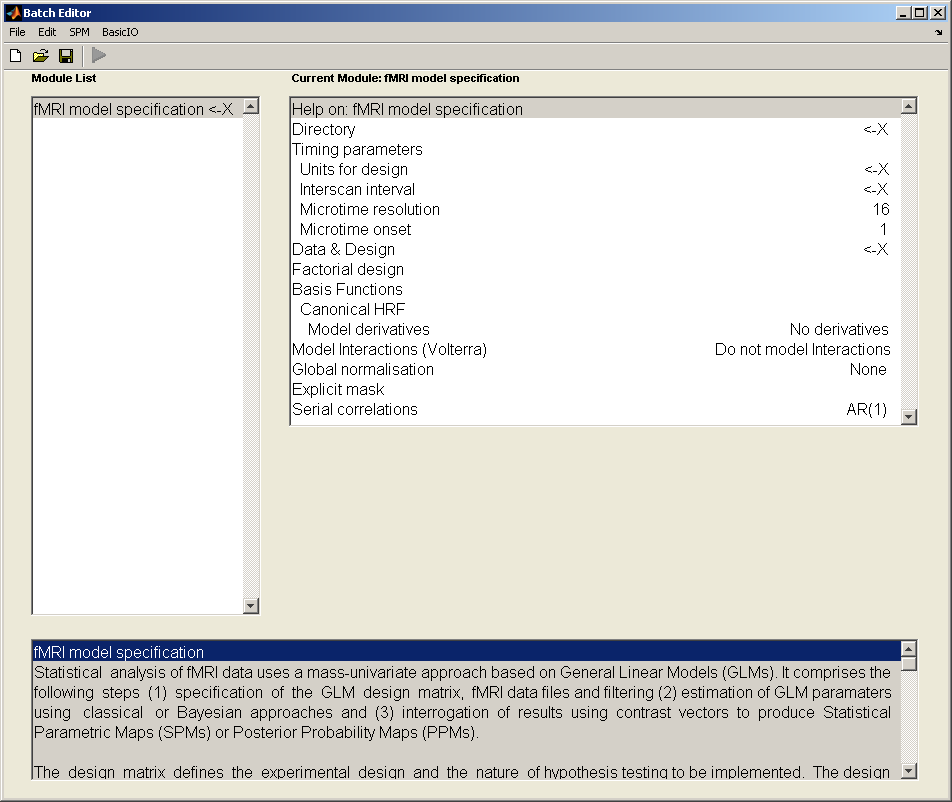
\includegraphics[width=100mm]{fmri_spec/fmri_model}
\end{center}
\caption{\em After starting SPM in fMRI mode, pressing the `Specify 1st-level' button, and then double-clicking on the `+fMRI model specification' text, the SPM graphics window should appear as above. The options under `-fMRI model specification' can be examined by clicking on them. A single click will bring up some help text in the lower subwindow (not shown in the above graphic). A double-click on options prefixed by a '+' will allow you to specify options at a greater level of detail. Options highlighted with a `$<$-X' are mandatory and must be filled in by the user. Each of the options shown above is described in this chapter. \label{spec}}
\end{figure}

In SPM, analysis of data from multiple subjects typically proceeds in two stages using models at two `levels'. The `first level' models are used to implement a within-subject analysis. Typically there will be as many first level models as there are subjects. Analysis proceeds as described using the `Specify first level' and `Estimate' options. The results of these analyses can then be presented as `case studies'. More often, however, one wishes to make inferences about the population from which the subjects were drawn. This is an example of a `Random-Effects (RFX) analysis' (or, more properly, a mixed-effects analysis). In SPM, RFX analysis is implemented using the `summary-statistic' approach where contrast images from each subject are used as summary measures of subject responses. These are then entered as data into a `second level' model. 

Figure~\ref{spec} shows how the SPM graphics window appears during fMRI model specification. 

\section{Timing parameters}

Specify various timing parameters needed to construct the design matrix. This includes the units of the design specification and the interscan interval.

Also, with long TRs you may want to shift the regressors so that they are aligned to a particular slice.  This is effected by changing the microtime resolution and onset. 

\subsection{Units for design}

The onsets of events or blocks can be specified in either scans or seconds.

\subsection{Interscan interval}

Interscan interval, TR, (specified in seconds).  This is the time between acquiring a plane of one volume and the same plane in the next volume.  It is assumed to be constant throughout.

\subsection{Microtime resolution}

In Echo-Planar Imaging (EPI), data is acquired a plane at a time. To acquire a whole volume of data takes at least a second or two.

It is possible, however, that experimental events may occur between scan (volume) acquisition times. This can be specified when building your design matrix either by (i) specifying your design in scans and using non-integer values  or (ii) specifying your design in seconds at a resolution greater than the TR.

SPM takes these timing specifications and builds its regressors using a `microtime' time-scale. The microtime resolution, t, is the number of time-bins per scan. 

Do not change this parameter unless you have a long TR and wish to shift regressors so that they are aligned to a particular slice. 

\subsection{Microtime onset}

The microtime onset, t0, is the first time-bin at which the regressors are resampled to coincide with data acquisition.  If t0 = 1 then the regressors will be appropriate for the first slice.  If you want to temporally realign the regressors so that they match responses in the middle slice then make t0 = t/2 (assuming there is a negligible gap between volume acquisitions).                                           

Do not change the default setting unless you have a long TR. 

A typical use of the t and t0 parameters is to set them to correspond to the results of any slice timing correction you have made eg. if you have 24 slices and have made slice 12 the reference slice you would set t=24, t0=12. 

\section{Data \& Design}

The design matrix defines the experimental design and the nature of hypothesis testing to be implemented.  The design matrix has one row for each scan and one column for each effect or explanatory variable. (e.g. regressor or stimulus function).  Figure~\ref{design} shows an example of a design matrix.

\begin{figure}
\begin{center}
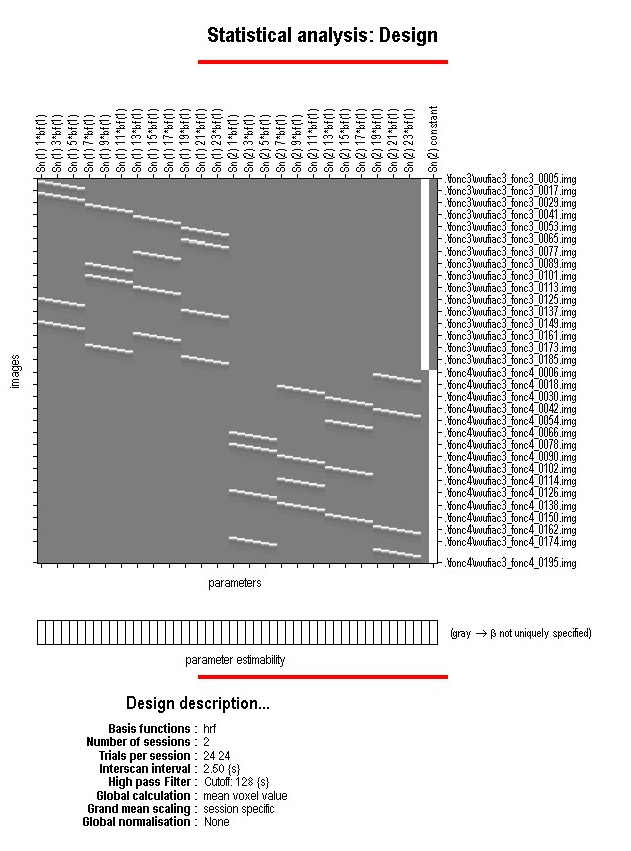
\includegraphics[width=100mm]{fmri_spec/design}
\end{center}
\caption{\em Design matrix for fMRI data from two sessions. There are 24 experimental conditions for each session. The last two columns model the average activity in each session, giving a total of 50 regressors. There are 191 fMRI scans for each session. The overall design matrix therefore has 382 rows and 50 columns. \label{design}}
\end{figure}

You can build design matrices with separable session-specific partitions.  Each partition may be the same (in which case it is only necessary to specify it once) or different.  Responses can be either event- or epoch related, where the latter model involves prolonged and possibly time-varying responses to state-related changes in experimental conditions.  Event-related response are modelled in terms of responses to instantaneous events.  Mathematically they are both modelled by convolving a series of delta (stick) or box-car functions, encoding the input or stimulus function. with a set of hemodynamic basis functions.

\subsection{Subject/Session}

The design matrix for fMRI data consists of one or more separable, session-specific partitions.  These partitions are usually either one per subject, or one per fMRI scanning session for that subject.

\subsubsection{Scans}

Select the fMRI scans for this session.  They must all have the same image dimensions, orientation, voxel size etc. This is implemented using SPM's file selector.

\subsubsection{Conditions}

You are allowed to combine both event- and epoch-related responses in the same model and/or regressor. Any number of condition (event or epoch) types can be specified.  Epoch and event-related responses are modeled in exactly the same way by specifying their onsets [in terms of onset times] and their durations.  Events are specified with a duration of 0.  If you enter a single number for the durations it will be assumed that all trials conform to this duration.For factorial designs, one can later associate these experimental conditions with the appropriate levels of experimental factors. 

\paragraph{Condition}

An array of input functions is constructed, specifying occurrence events or epochs (or both). These are convolved with a basis set at a later stage to give regressors that enter into the design matrix. Interactions of evoked responses with some parameter (time or a specified variate) enter at this stage as additional columns in the design matrix with each trial multiplied by the [expansion of the] trial-specific parameter. The 0th order expansion is simply the main effect in the first column.

\subparagraph{Name}

Condition Name

\subparagraph{Onsets}

Specify a vector of onset times for this condition type. This can be entered using the keyboard eg. typing in `100 300' and then hitting return or `100;300' or `[100,300]' or `[100,300]''.

More usually, however, this specification takes place using variables that have been created before and loaded into matlab. For example, an \verb!my_onsets! cell array\footnote{Cell arrays are usually used in preference to matrices as different event types can then have different numbers of events.} might exist in a file you created earlier called \verb!my_design.mat!. You would then type \verb!load my_design! at the matlab command prompt before pressing the `Specify 1st-level' button. 

You could then specify the onsets for condition 2 by typing in eg. \verb!my_onsets{2}! instead of entering the numbers via the keyboard.


\subparagraph{Durations}

Specify the event durations (in seconds). Epoch and event-related responses are modeled in exactly the same way but by specifying their different durations.  Events are specified with a duration of 0.  If you enter a single number for the durations it will be assumed that all trials conform to this duration. If you have multiple different durations, then the number must match the number of onset times.

\subparagraph{Time Modulation}

This option allows for the characterisation of nonstationary responses.  Specifically, you can model either linear or nonlinear time effects. For example, 1st order modulation would model the stick functions and a linear change of the stick function heights over time. Higher order modulation will introduce further columns that contain the stick functions scaled by time squared, time cubed etc.

\subparagraph{Parametric Modulations}

The stick function itself can be modulated by some parametric variate (this can be time or some trial-specific variate like reaction time) modeling the interaction between the trial and the variate. The events can be modulated by zero or more parameters.

See \cite{parametric_pet,parametric_fmri} for further details of parametric modulations.

\subsubsection{Multiple conditions}

If you have multiple conditions then entering the details a condition at a time is very inefficient. This option can be used to load all the required information in one go. 

You will need to create a \verb!*.mat! file containing the relevant information. This \verb!*.mat! file must include the following cell arrays: names, onsets and durations eg. \verb!names{2}='SSent-DSpeak'!, \verb!onsets{2}=[3 5 19 222]!, \verb!durations{2}=[0 0 0 0]! contain the required details of the second condition. These cell arrays may be made available by your stimulus delivery program eg. COGENT. The duration vectors can contain a single entry if the durations are identical for all events. 

You then need to use SPM's file selector to select this \verb!*.mat! file.

\subsubsection{Regressors}

Regressors are additional columns included in the design matrix, which may model effects that would not be convolved with the haemodynamic response.  One such example would be the estimated movement parameters, which may confound the data.

\paragraph{Regressor}

\subparagraph{Name}

Enter name of regressor eg. First movement parameter

\subparagraph{Value}

Enter the values that the regressor takes. This could also be, for example, the name of a variable in MATLAB's work space that you have previously loaded in from a file. This might be a subjects movement parameters or reaction times.

\subsubsection{Multiple regressors}

If you have mutliple regressors eg. realignment parameters, then entering the details a regressor at a time is very inefficient. This option can be used to load all the required information in one go. 

You will first need to create a *.mat file containing a matrix R. Each column of R will contain a different regressor. When SPM creates the design matrix the regressors will be named R1, R2, R3, ..etc.

You then need to use SPM's file selector to select this \verb!*.mat! file.

\subsubsection{High-pass filter}

The default high-pass filter cutoff is 128 seconds. Slow signal drifts with a period longer than this will be removed. Use `Explore design' to ensure this cut-off is not removing too much experimental variance. This is described later in section~\ref{explore}. High-pass filtering is implemented using a residual forming matrix (i.e. it is not a convolution) and is simply a way to remove confounds without estimating their parameters explicitly.  The constant term is also incorporated into this filter matrix.

\section{Factorial design}

If you have a factorial design then SPM can automatically generate the contrasts necessary to test for the main effects and interactions. 

This includes the F-contrasts necessary to test for these effects at the within-subject level (first level) and the simple contrasts necessary to generate the contrast images for a between-subject (second-level) analysis.

To use this option, create as many factors as you need and provide a name and number of levels for each.  SPM assumes that the condition numbers of the first factor change slowest, the second factor next slowest etc. It is best to write down the contingency table for your design to ensure this condition is met. This table relates the levels of each factor to the conditions. 

For example, if you have 2-by-3 design  your contingency table has two rows and three columns where the the first factor spans the rows, and the second factor the columns. The numbers of the conditions are 1,2,3 for the first row and 4,5,6 for the second. 

See \cite{rnah_anova} for more information on SPM and factorial designs.

\subsection{Factor}

Add a new factor to your experimental design

\subsubsection{Name}

Name of factor, eg. 'Repetition' 

\subsubsection{Levels}

Enter number of levels for this factor, eg. 2

\section{Basis Functions}

SPM uses basis functions to model the hemodynamic response. This could be a single basis function or a set of functions. The most common choice is the `Canonical HRF' with or without time and dispersion derivatives. 

\subsection{Canonical HRF}

Canonical Hemodynamic Response Function (HRF). This is the default option. Contrasts of these effects have a physical interpretation and represent a parsimonious way of characterising event-related responses. This option is also useful if you wish to look separately at activations and deactivations. This is implemented using a t-contrast with a +1 or -1 entry over the canonical regressor. 

\subsubsection{Model derivatives}

Model HRF Derivatives. The canonical HRF combined with time and dispersion derivatives comprise an `informed' basis set, as the shape of the canonical response conforms to the hemodynamic response that is commonly observed. The incorporation of the derivative terms allow for variations in subject-to-subject and voxel-to-voxel responses. The time derivative allows the peak response to vary by plus or minus a second and the dispersion derivative allows the width of the response to vary by a similar amount. 

A positive estimate of the time-derivative regression coefficient implies that the peak hemodynamic response occurs later than usual ie. than would be expected using just the canonical regressor. A positive estimate for the dispersion derivative implies a more dispersed response than usual.

The informed basis set requires an SPM{F} for inference. T-contrasts over just the canonical are perfectly valid but assume constant delay/dispersion. The informed basis set compares favourably with eg. FIR bases on many data sets \cite{rnah_basis}.

\subsection{Other basis sets}

The other basis sets supported by SPM are

\begin{enumerate}
\item{Fourier Set}
\item{Fourier Set (Hanning)}
\item{Gamma Functions}
\item{Finite Impulse Response (FIR)}
\end{enumerate}

For each of these options you must also specify the {\bf window length} which is the length in seconds of the post-stimulus time window that the basis functions span. You must also specify the {\bf order}, that is, how many basis functions to use.

Usually, an informed basis set should be sufficient for most data sets. If this does not provide a good fit to the data it may be worthwhile re-considering how the neuronal events are modelled ie. is the timing correct ? should events be split into subsets ? 

Alternatively, the gamma basis functions are an interesting choice as a particular linear combination of them is actually used to specify the canonical HRF. The FIR approach is of interest as it is equivalent to the method of `selective averaging'. See \cite{rnah_conv} for further details. 

\section{Model Interactions (Volterra)}

Generalized convolution of inputs, $U$, with basis set, $bf$.

For first order expansions the causes are simply convolved (e.g. stick functions) in $U$ by the basis functions in $bf$ to create a design matrix $X$.  For second order expansions new entries appear that correspond to the interaction among the original causes. The basis functions for these effects are two dimensional and are used to assemble the second order kernel. 

Interactions or response modulations can enter at two levels.  Firstly the stick function itself can be modulated by some parametric variate. This can be time or some trial-specific variate like reaction time modeling the interaction between the trial and the variate. Secondly interactions among the trials themselves can be modeled using a Volterra series formulation that accommodates interactions over time (and therefore within and between trial types). 

This last option is useful for accommodating nonlinearities in the hemodynamic response. For example, if two events occur within a second or so of each other then the hemodynamic response to the pair may be less than the sum of the responses to each event when occuring in isolation. This type of `sub-linear' response can be modelled using Volterra kernels. See \cite{balloon} for further details.

\section{Directory}

Select a directory where the SPM.mat file containing the specified design matrix will be written. If this directory already contains an SPM.mat file then SPM will warn you of this before overwriting it, when the specification job is run.

\section{Global normalisation}

SPM can normalise fMRI data in one of two ways. These are selected using the options `None' (the default) and `Scaling'. 

Both methods are based on first estimating the average within-brain fMRI signal, $g_{ns}$, where $n$ denotes scan and $s$ denotes session. If you select `Scaling', SPM will multiply each fMRI value in scan $n$ and session $s$ by $100/g_{ns}$.

If you select `None' then SPM computes the grand mean value, $g_s=\frac{\sum_{n=1}^N g_{ns}}{N}$ where N is the number of scans in that session. This is the fMRI signal averaged over all voxels within the brain and all time points within session $s$. SPM then implements `Session-specific grand mean scaling' by multiplying each fMRI data point in session $s$ by $100/g_s$. 
 
See \cite{ja_global} for further discussion of this issue.

\section{Explicit mask}

Specify an image for explicitly masking the analysis. A sensible option here is to use a segmentation of structural images to specify a within-brain mask. If you select that image as an explicit mask then only those voxels in the brain will be analysed. This both speeds the estimation and restricts SPMs/PPMs to within-brain voxels. Alternatively, if such structural images are unavailable or no masking is required, then leave this field empty.

\section{Serial correlations}

Serial correlations in fMRI time series due to aliased biorhythms and unmodelled neuronal activity can be accounted for using an autoregressive AR(1) model during Classical (ReML) parameter estimation.  

This estimate assumes the same correlation structure for each voxel, within each session.  ReML estimates are then used to correct for non-sphericity during inference by adjusting the statistics and degrees of freedom appropriately.  The discrepancy between estimated and actual correlations are greatest at low frequencies.  Therefore specification of the high-pass filter is particularly important.                                                                                             

Serial correlation can be ignored if you choose the `none' option. Note that the above options only apply if you later specify that your model will be estimated using the Classical (ReML) approach. If you choose Bayesian estimation these options will be ignored. For Bayesian estimation, the choice of noise model (AR model order) is made under the estimation options. See \cite{peb1,vb_fmri_ar} for further discussion of these issues.

\section{Reviewing your design \label{explore}}

After you have completed the SPM `job' file for specifying your fMRI design, and have run it, you will then be able to review your design by pressing the `Review' button in SPM's button window (the top-left window). This is particularly useful, for example, for checking that your experimental variance has not been removed by high-pass filtering, as shown in Figure~\ref{rev4}.

\begin{figure}
\begin{center}
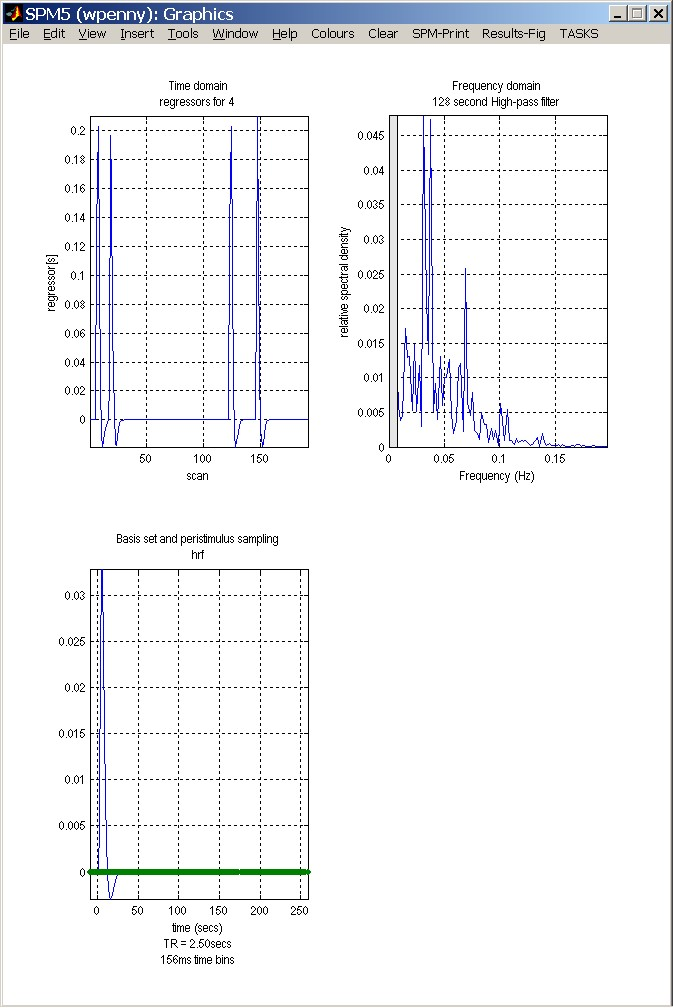
\includegraphics[width=100mm]{fmri_spec/reg4}
\end{center}
\caption{\em After pressing `Review', selecting the pull-down `Design' menu, Explore-$>$Session, and selecting the regressor you wish to look at, you should get a plot similar to the one above. The top row shows time and frequency domain plots of the time-series corresponding to this regressor. In this particular case we have four events. Each event or `stick function' has been convolved with the hemodynamic response function shown in the bottom panel. The frequency domain graph is useful for checking that experimental variance is not removed by high-pass filtering. The grayed out section of the frequency plot shows those frequencies which are removed. For this regressor we have plenty of remaining experimental variance (see the peak at about 0.04Hz). \label{rev4}}
\end{figure}

\chapter{fMRI model estimation \label{Chap:fmri_est}}

Model parameters can be estimated using classical (ReML - Restricted Maximum Likelihood) or Bayesian algorithms. After parameter estimation, the RESULTS button can be used to specify contrasts that will produce Statistical Parametric Maps (SPMs), Effect Size Maps (ESMs) or Posterior Probability Maps (PPMs) and tables of statistics. 

\section{Select SPM.mat}

Select the SPM.mat file that contains the design specification. SPM will output the results of its analysis into this directory. This includes overwriting the SPM.mat file. When the estimation job is run, no warning will be given that the SPM.mat file will be overwritten. A warning is given at the specification stage. When it comes to estimation, SPM assumes that you've now sorted out your directory structures.

\begin{figure}
\begin{center}
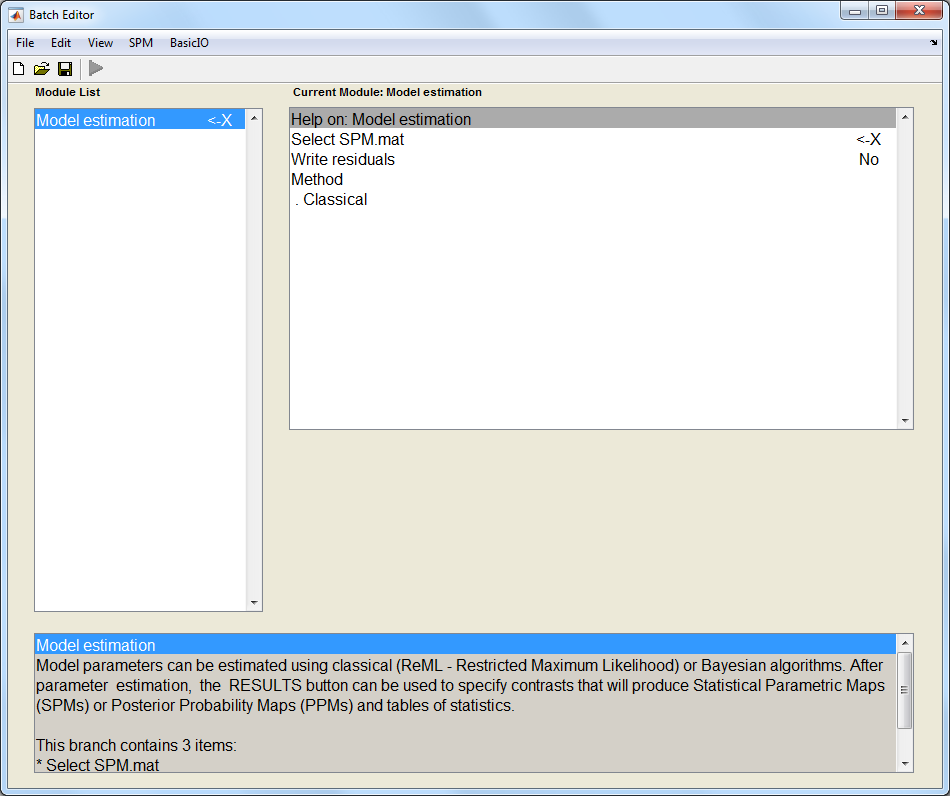
\includegraphics[width=100mm]{fmri_est/est_method}
\end{center}
\caption{\em After starting SPM in fMRI mode, pressing the `Estimate' button, and then double-clicking on the `+fMRI model estimation' text, the SPM graphics window should appear as above. The options under `-fMRI model estimation' can be examined by clicking on them. A single click will bring up some help text in the lower subwindow (not shown in the above graphic). A double-click on options prefixed by a '+' will allow you to specify options at a greater level of detail. Options highlighted with a `$<$-X' are mandatory and must be filled in by the user. Each of the options shown above is described in this chapter. \label{est}}
\end{figure}

\section{Method}

There are three possible estimation procedures for fMRI models (1) classical (ReML) estimation of first or second level models, (2) Bayesian estimation of first level models and (3) Bayesian estimation of second level models. Option (2) uses a Variational Bayes (VB) algorithm that is new to SPM5. Option (3) uses the Empirical Bayes algorithm with global shrinkage priors that was also in SPM2. 

To use option (3) you must have already estimated the model using option (1). That is, for second-level models you must run a ReML estimation before running a Bayesian estimation. This is not necessary for option (2). Bayesian estimation of 1st-level models using VB does not require a prior ReML estimation.

\subsection{Classical}

Model parameters are estimated using Restricted Maximum Likelihood (ReML). This assumes the error correlation structure is the same at each voxel. This correlation can be specified using either an AR(1) or an Independent and Identically Distributed (IID) error model. These options are chosen at the model specification stage. ReML estimation should be applied to spatially smoothed functional images. See \cite{peb1,peb2} for further details of the ReML estimation scheme. After estimation, specific profiles of parameters are tested using a linear compound or contrast with the T or F statistic. The resulting statistical map constitutes an SPM. The SPM{T}/{F} is then characterised in terms of focal or regional differences by assuming that (under the null hypothesis) the components of the SPM (ie. residual fields) behave as smooth stationary Gaussian fields.

The rest of this chapter describes the Bayesian estimation options. So, please skip to the next chapter if you are interested only in classical estimation and inference. 

\subsection{Bayesian 1st-level}

Model parameters are estimated using Variational Bayes (VB). This allows you to specify spatial priors for regression coefficients and regularised voxel-wise AR(P) models for fMRI noise processes. The algorithm does not require functional images to be spatially smoothed. Estimation will take about 5 times longer than with the classical approach. This is why VB is not the default estimation option. The VB approach has been described in a number of papers \cite{vb_fmri_ar,vb2,vb3,will_bayes_srglm}.
                                                          
After estimation, contrasts are used to find regions with effects larger than a user-specified size eg. 1 per cent of the global mean signal. These effects are assessed statistically using a Posterior Probability Map (PPM) \cite{karl_posterior}.

\begin{figure}
\begin{center}
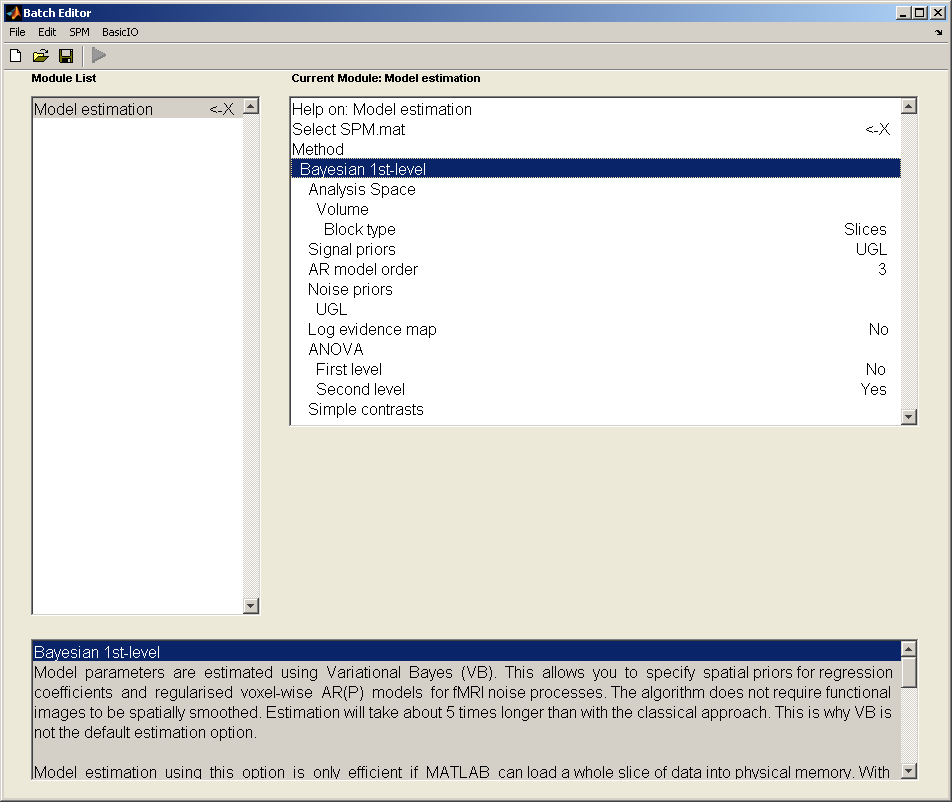
\includegraphics[width=100mm]{fmri_est/bayes_options}
\end{center}
\caption{\em After choosing Bayesian 1st-level under `Method' and then double-clicking on the `+Bayesian 1st-level' text, the SPM graphics window should appear as above. Each of the options shown above is described in this chapter. \label{bayes_options}}
\end{figure}

\subsubsection{Analysis Space}

Because estimation can be time consuming, an option is provided to analyse selected slices rather than the whole volume.

\paragraph{Volume}

You have selected the Volume option. SPM will analyse fMRI time series in all slices of each volume.

\paragraph{Slices}

Enter Slice Numbers. This can be a single slice or multiple slices. If you select a single slice or only a few slices you must be aware of the interpolation options when, after estimation, displaying the estimated images eg. images of contrasts or AR maps. The default interpolation option may need to be changed to nearest neighbour (NN) (see bottom right hand of graphics window) for your slice maps to be visible.

\subsubsection{Signal priors}

\begin{itemize}

\item{[GMRF] Gaussian Markov Random Field. This spatial prior is the recommended option. Regression coefficients at a given voxel are (softly) constrained to be similar to those at nearby voxels. The strength of this constraint is determined by a spatial precision parameter that is estimated from the data. Different regression coefficients have different spatial precisions allowing each putative experimental effect to have its own spatial regularity. }

\item{[LORETA] Low Resolution Tomography Prior. This spatial prior is very similar to the GMRF prior and is a standard choice for MEG/EEG source localisation algorithms. It does, however, have undesirable edge effects.}                                                                                                    

\item{[Global] Global Shrinkage prior. This is not a spatial prior in the sense that regression coefficients are constrained to be similar to neighboring voxels. Instead, the average effect over all voxels (global effect) is assumed to be zero and all regression coefficients are shrunk towards this value in proportion to the prior precision. This is the same prior that is used for Bayesian estimation at the second level (see also \cite{karl_posterior}), except that here the prior precision is estimated separately for each slice. }

\item{[Uninformative] A flat prior. Essentially, no prior information is used. If you select this option then VB reduces to Maximum Likelihood (ML) estimation. This option is useful if, for example, you do not wish to use a spatial prior but wish to take advantage of the voxel-wise AR(P) modelling of noise processes. In this case, you would apply the algorithm to images that have been spatially smoothed. For P=0, ML estimation in turn reduces to Ordinary Least Squares (OLS) estimates, and for P$>$0, ML estimation is equivalent to a weighted least squares (WLS) algorithm but where the weights are different at each voxel. This reflects the different noise correlations at each voxel. }

\end{itemize}

\subsubsection{AR model order}

An AR model order of 3 is the default. Cardiac and respiratory artifacts are periodic in nature and therefore require an AR order of at least 2. In previous work, voxel-wise selection of the optimal model order showed that a value of 3 was the highest order required \cite{vb_fmri_ar}.

Higher model orders have little effect on the estimation time. If you select a model order of zero this corresponds to the assumption that the errors are Independent and Identically Distributed (IID). This AR specification overrides any choices that were made in the model specification stage.

Voxel-wise AR models are fitted separately for each session of data. For each session this therefore produces maps of AR(1), AR(2) etc coefficients in the output directory. 

\subsubsection{Noise priors}

There are three noise prior options.

\begin{itemize}

\item{[GMRF] Gaussian Markov Random Field. This is the default option. This spatial prior is the same as that used for the regression coefficients. Spatial precisions are estimated separately for each AR coefficient eg. the AR(1) coefficient over space, AR(2) over space etc.}

\item{[LORETA] Low Resolution Tomography Prior. See comments on LORETA priors for regression coefficients.}

\item{[Tissue-type] This provides an estimation of AR coefficients at each voxel that are biased towards typical values for that tissue type (eg. gray, white, CSF). If you select this option you will need to then select files that contain tissue type maps (see below). These are typically chosen to be Grey Matter, White Matter and CSF images derived from segmentation of registered structural scans.}

\end{itemize}
                                                                                                            
Previous work has shown that there is significant variation in AR values with tissue type. However, GMRF priors have previously been favoured by Bayesian model comparison \cite{will_bayes_srglm}.

\subsubsection{ANOVA}

Perform 1st or 2nd level Analysis of Variance.

\paragraph{First level}

This is implemented using Bayesian model comparison as described in \cite{will_bayes_srglm}. For example, to test for the main effect of a factor two models are compared, one where the levels are represented using different regressors and one using the same regressor. This therefore requires explicit fitting of several models at each voxel and is computationally demanding (requiring several hours of computation). The recommended option is therefore NO.

To use this option you must have already specified your factorial design during the model specification stage. 

\paragraph{Second level}

This option tells SPM to automatically generate the simple contrasts that are necessary to produce the contrast images for a second-level (between-subject) ANOVA. Naturally, these contrasts can also be used to characterise simple effects for each subject. 

With the Bayesian estimation option it is recommended that contrasts are computed during the parameter estimation stage (see 'simple contrasts' below). The recommended option here is therefore YES.

To use this option you must have already specified your factorial design during the model specification stage. 

If you wish to use these contrast images for a second-level analysis then you will need to spatially smooth them to take into account between-subject differences in functional anatomy ie. the fact that one persons V5 may be in a different position than anothers. 

\subsubsection{Simple contrasts}

`Simple' contrasts refers to a contrast that spans one-dimension ie. to assess an effect that is increasing or decreasing.

If you have a factorial design then the contrasts needed to generate the contrast images for a 2nd-level ANOVA (or to assess these simple effects within-subject) can be specified automatically using the ANOVA-$>$Second level option.

When using the Bayesian estimation option it is computationally more efficient to compute the contrasts when the parameters are estimated. This is because estimated parameter vectors have potentially different posterior covariance matrices at different voxels and these matrices are not stored. If you compute contrasts post-hoc these matrices must be recomputed. This uses an approximate reconstruction based on a Taylor series expansion described in \cite{vb3}. It is therefore recommended to specify as many contrasts as possible prior to parameter estimation.

If you wish to use these contrast images for a second-level analysis then you will need to spatially smooth them to take into account between-subject differences in functional anatomy ie. the fact that one persons V5 may be in a different position than anothers. 

\paragraph{Simple contrast}

\subparagraph{Name}

Name of contrast eg. `Positive Effect'

\subparagraph{Contrast vector}

These contrasts are used to generate PPMs which characterise effect sizes at each voxel. This is different to SPMs in which eg. maps of t-statistics show the ratio of the effect size to effect variability (standard deviation). SPMs are therefore a-dimensional. This is not the case for PPMs as the size of the effect is of primary interest. Some care is therefore needed about the scaling of contrast vectors. For example, if you are interested in the differential effect size averaged over conditions then the contrast $[0.5, 0.5, -0.5, -0.5]$ would be more suitable than the $[1, 1, -1, -1]$ contrast which looks at the differential effect size summed over conditions. 

\subsection{Bayesian 2nd-level}

Bayesian estimation of 2nd level models. This option uses the Empirical Bayes algorithm with global shrinkage priors that was previously implemented in SPM2. It is described in detail in \cite{karl_posterior}.

Use of the global shrinkage prior embodies a prior belief that, on average over all voxels, there is no net experimental effect. Some voxels will respond negatively and some positively with a variability determined by the prior precision. This prior precision can be estimated from the data using Empirical Bayes. 

\section{Output files}

After estimation a number of files are written to the output directory. These are

\begin{itemize}
\item{An \verb!SPM.mat! file containing specification of the design and estimated model parameters}
\end{itemize}

\subsection{Classical 1st-level}

For classical 1st-level models the following files are also produced

\begin{itemize}

\item{Images of estimated regression coefficients  \verb!beta_000k.img! where $k$ indexes the $k$th regression coefficient.}

\item{An image of the variance of the error \verb!ResMS.img!.}

\item{An image \verb!mask.img! indicating which voxels were included in the analysis.}

\item{The image \verb!RPV.img!, the estimated resels per voxel.}

\item{If contrasts have been specified SPM also writes \verb!con_000i.img!  if the $i$th contrast is a t-contrast and the extra sum of squares image \verb!ess_000i.img! if it is an F-contrast.} 

\end{itemize}

Type \verb!help spm_spm! at the matlab command prompt for further information.

\subsection{Bayesian 1st-level}

For Bayesian 1st-level models the following files are also produced

\begin{itemize}

\item{Images of estimated regression coefficients  \verb!Cbeta_000k.img! where $k$ indexes the $k$th regression coefficient. These filenames are prefixed with a `C' indicating that these are the mean values of the `Conditional' or `Posterior' density.}

\item{Images of error bars/standard deviations on the regression coefficients \verb!SDbeta_000k.img!.}

\item{An image of the standard deviation of the error \verb!Sess1_SDerror.img!.}

\item{An image \verb!mask.img! indicating which voxels were included in the analysis.}

\item{If a non-zero AR model order is specified then SPM also writes images \verb!Sess1_AR_000p.img! where $p$ indexes the $p$th AR coefficient.}

\item{If contrasts have been specified SPM also writes \verb!con_000i.img! and \verb!con_sd_000i.img! which are the mean and standard deviation of the $i$th pre-defined contrast.} 

\end{itemize}

Each of these images can be inspected using the `Display' button. Type \verb!help spm_spm_vb! at the matlab command prompt for further information.

\section{Model comparison}

Once you have estimated a model you can use SPM's results button to look at the results. You can also extract fMRI data from regions of interest using the ROI button. You can then compare GLMs based on different hemodynamic basis sets using the Bayesian model evidence. 

This is described in \cite{will_bayes_srglm} and implemented using the command line option `spm\_vb\_roi\_basis'. This requires a VOI filename (created using the ROI button) and an SPM data structure. Type `help spm\_vb\_roi\_basis' at the matlab command prompt for further information. Figure~\ref{basis} shows an example output from the function indicating that, for the data in this brain region, an informed basis set has the highest model evidence.

\begin{figure}
\begin{center}
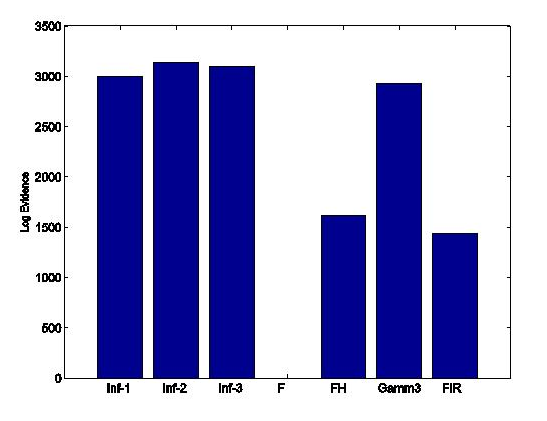
\includegraphics[width=150mm]{fmri_est/basis}
\end{center}
\caption{\em This plot shows the model evidence for a number of different hemodynamic basis sets: Inf1 - Canonical HRF, Inf2 - Canonical plus temporal derivative, Inf3 - Canonical plus temporal and dispersion derivatives, F - Fourier, FH - Fourier with a Hanning Window, Gamm3 - 3 Gamma basis functions and FIR - a Finite Impulse Response function. An informed basis set provides the best model of the data for the selected region.  \label{basis}}
\end{figure}

%\include{con}
\include{factorial_design}

%%%%%% M/EEG %%%%%%
\part{EEG/MEG}
\chapter{SPM for EEG/MEG overview}
\label{ch:eeg_overview}
Unlike previous versions, SPM5 provides for
the analysis of EEG and MEG data. The initial main motivation for this big
leap came from the insight that any integration of modalities like
fMRI and EEG should be based on a common theoretical and practical
basis. Historically, research into fMRI and EEG/MEG models and
analysis has been quite divorced. The same is partially true for the
EEG and MEG field. It is our hope that SPM5 provides a common analysis
ground for modellers and experimentalists of both the PET/fMRI and 
EEG/MEG fields.
\\

SPM for EEG/MEG was primarily developed for the analysis of epoched
data. This is because we are mostly interested in experiments which
perturb the system with a designed stimulus. The analysis of
continuous data is typically performed for experiments without
designed stimuli like in sleep or epilepsy research. Note that although
SPM5 does not provide for an analysis of continuous data per se, many
SPM5 routines can be used for these data.
\\

SPM for EEG/MEG can be partitioned into four parts. These are (i)
preprocessing, (ii) projection to voxel-space/source reconstruction,
(iii) statistical analysis, and (iv) Dynamical Causal Modelling (DCM). 

The preprocessing functions provide for simple operations that are
standard in other software packages. 

The projection to voxel-space is a critical step. When using a source
reconstruction, it takes the analysis to brain space. But even when
using a simple projection to some 2D-sensor plane, we can then use SPM
functions and concepts that were developed for voxel-based data. The
projection to a 2D-plane is performed using a simple interpolation and
is mostly equivalent to widely used sensor-based analyses. The source
reconstruction to brain space is based on models that assume many
distributed dipoles in brain space. Solutions to these models
typically show dispersed activity and are well-suited for SPM
mass-univariate analysis approach.
\\

The statistical analysis is one of the strong points of SPM. PET/fMRI
users already familiar with the graphical representation of
general linear models won't have difficulties to use SPM for the
analysis of EEG/MEG data. SPM5 provides for a comprehensive range of
classical linear models that can be used to model the data. These
models are basically the same as used in the EEG/MEG field
for random effects analyses of multiple subjects. In SPM, we assume
that the data in voxel-space is a sampled version of some continuous Gaussian
random field. This allows us to use Random field theory (GFT)
for the correction of multiple comparisons to control family-wise
error over voxels. The GFT approach has the advantage that
super-threshold maxima are assessed for their significance, whereas
conventional approaches have to specify a-priori the locations of
expected activations.
\\

Dynamical Causal Modelling (DCM) is a departure from the mass-univariate
approach and is an extension of the SPM software package. DCM for ERP/ERFs is a
generative model for evoked responses. The observed data is modelled
as the spatiotemporal expression of a small hierarchical network that
responds to a stimulus. Differences between evoked responses due to different
stimuli are modelled as modulations of the coupling between specific
areas. Importantly, this approach is based on a neurobiologically
grounded model. This allows us to obtain parameter estimates that have
some physiological interpretation.
\\

The following chapters will go through all the EEG/MEG related
functionality of SPM5. All users will probably find the tutorial
useful for a quick start. A further detailed description of the
preprocessing functions is given in chapter
\ref{ch:eeg_preprocessing}. The 3D-source reconstruction is described
in chapter \ref{ch:eeg_imaging} and some dipole fitting technique in
chapter \ref{ch:eeg_ecd}. In chapter \ref{ch:eeg_stats}, we
guide you through the modelling of M/EEG data at the first and second
level of a hierarchical linear model. Finally, in chapter
\ref{ch:eeg_DCM}, we describe the graphical user interface for
dynamical causal modelling for evoked 
responses, i.e.~event-related potentials (ERPs) and event-related
fields (ERFs).


\chapter{EEG/MEG preprocessing --- Tutorial}
\label{ch:eeg_tutorial}
This tutorial will give a users guide to the pre-processing sections
of SPM M/EEG. We will use an example data set collected on a 128 active
electrode Biosemi EEG system. This data set is available from the SPM
website. The data was recorded continuously and had three event types
(event identifiers 1,2 and 4) These event types indicated the type of
visual stimulus presented.

\section{ERP analysis}

\subsection{Convert}
Convert reads the EEG data file and writes the data in a format that
is used for SPM analysis. The SPM format has two components a *.mat
and *.dat file. The *.mat file contains the data structure D and the
*.dat is the M/EEG data.\\

After clicking on Convert you will be asked to select the format of
your EEG or MEG data. For the example data set we select BDF. Next
select the data file. For the example data we select the
EEGexample.bdf. Next select the data template file from the EEG
template file. This file contains a template of electrode positions in
2D. For the example data set select the bdf\_setup.mat.\\

NB the questions then asked depend upon the data format selected. Here
we will only address the questions for the BDF format of the example
data set. 

For BDF files the HEOG, VEOG and any other additional recordings are
saved in the EXG channels. Here we attribute labels to these
recordings. For the example data set we recorded HEOG (EXG 3 4), VEOG
(EXG 4 5) and recorded from the earlobes (EXG 1 2) to allow
re-referencing offline. No other additional data were
recorded. Therefore we enter the following:

\begin{figure}
\begin{center}
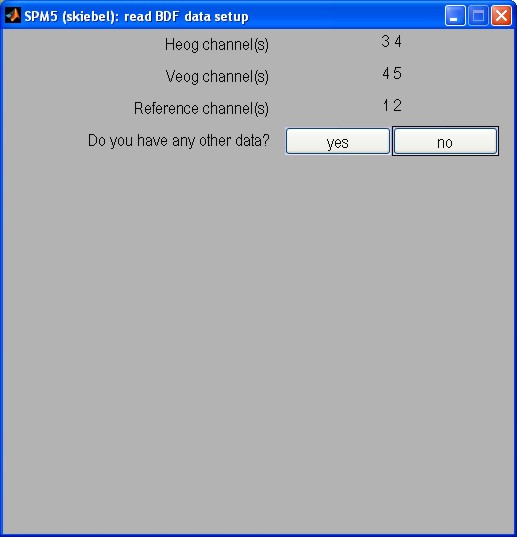
\includegraphics[width=100mm]{meeg/tutorial1}
\end{center}
\caption{\em Specifying the options for converting bdf-files} 
\end{figure}

The Convert function writes an EEGexample.mat and an EEGexample.dat
file in the current directory.

\subsection{Epoch}
To epoch the data click on epoching. Select the EEG mat file to
epoch. Choose the peri-stimulus time window. Choose the events to
epoch. Possible events will be listed in the Matlab command window. If
you do not have any events in you converted data file you can input
them in by reading in a new event list.

For the example data set exampleEEG.mat was selected and the following
parameters were used:

\begin{figure}
\begin{center}
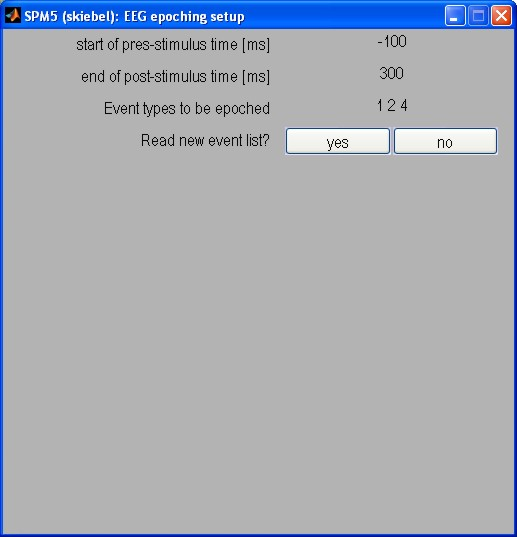
\includegraphics[width=100mm]{meeg/tutorial2}
\end{center}
\caption{\em Specifying the options for epoching the example data} 
\end{figure}

Having epoched the data one could filter and downsample the epoched data as above.
Epoching writes a *.mat and *.dat file prefixed by a 'e\_'. 

\subsection{Filter}
Filter filters the data using a Butterworth filter. This can be
applied either before or after epoching (see 1.3). Here it is applied
after. 

After clicking Filter select the *.mat file produced by Convert. For
the example data set select e\_EEGexample.mat. 

Next select the filter type, either lowpass or bandpass. If lowpass is
selected enter the cut-off frequency. If bandpass is selected enter
the two frequencies that specify the band of interest. \\ 

The Filter function writes a *.mat and *.dat file prefixed by a 'f'. \\

For the example data set e\_exampleEEG.mat was selected and a bandpass
filter was used from 0.1-45 Hz.


\subsection{Downsample}
To downsample the data select downsample from the 'Other' pull-down
menu. Select the data file to downsample. Enter the new sampling
rate. For the example dataset we downsampled to 100 Hz. Downsample
writes a *.mat and *.dat file prefixed by a 'd'.

For the example data set fe\_exampleEEG.mat was selected.

\subsection{Artefacts}
Two different methods of artefact removal are implemented in SPM5. One
is a simple thresholding method. The other uses a robust averaging
methodology to weight each time point by a function of the residuals. 

To remove artefacts click on Artefacts. Select the epoched data file
to analyse. If you know of bad trials or electrodes that you noted
during acquisition or found using another methodology you can read
them in using the 'read own artefact list'. If you want to use robust
averaging click yes to the following question if not click no. To
threshold channels click yes and then enter the threshold you wish to
use. The thresholding has two passes. One to find bad electrodes and
the second to find bad trials. If robust averaging was selected the
second pass will apply the robust averaging approach but a first pass
could use a thresholding method to find the bad electrodes prior to
robust averaging.\\

Artefacts writes a *.mat and *.dat file prefixed by an 'a'.\\ 

\begin{figure}
\begin{center}
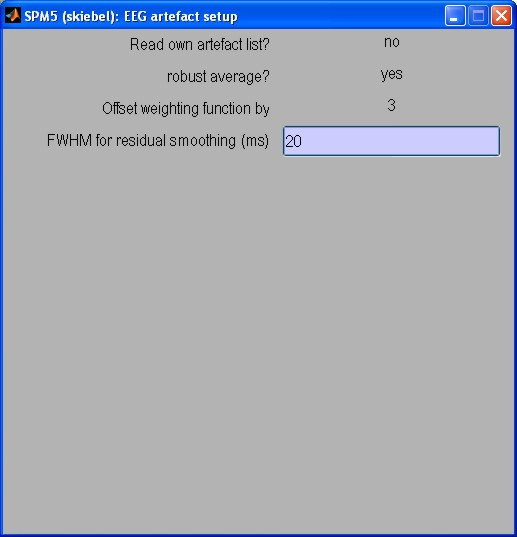
\includegraphics[width=100mm]{meeg/tutorial3}
\end{center}
\caption{\em Specifying the options for artefact detection in the
  example data}
\end{figure}

For the example data set dfe\_exampleEEG.mat was selected. No artefact
list was used and robust averaging was selected with a threshold of
100  v. For the robust averaging the default parameters were used.

\subsection{Averaging}
To produce a mean ERP click on averaging and select the EEG mat file
that you wish to average. This will automatically average either
ignoring the bad channels and trials or it will apply the weighting
matrix calculated from robust averaging. For the example data set
adfe\_exampleEEG.mat was selected.\\

Averaging writes a *.mat and *.dat file prefixed by an 'm'. 

\section{Other useful functions}
\subsection{Time-Frequency}
In SPM5 it is possible to apply a time-frequency analysis to the
data. This can either be applied to the averaged ERP to produce
time-frequency plot of evoked oscillations. Or it can be applied to
each trial and then averaged across trials to produce time-frequency
plot of evoked oscillations and induced oscillations. To produce
time-frequency plots select time-frequency from the other pull-down
menu. Select the EEG mat file to analyse. Enter a vector containing
the frequencies that you wish to analyse. You are then given the
option to baseline correct the time-frequency data. Next enter the
Morlet wavelet factor that you wish to use. The default value is
7. Next you can select the channels you wish to analyse. The default
is all channels.\\

Time-Frequency writes two *.mat and *.dat files. The first, the power,
is prefixed by 't1'. The second, the phase, is  prefixed by 't2'.

\subsection{Average TF}
To average time-frequency data sets across trials select average TF
from the other pull down menu. Select the T1*.mat EEG mat file to
average. As with the Averaging function Average TF writes a *.mat and
*.dat file prefixed by an 'm'.
\chapter{EEG/MEG preprocessing -- Reference \label{Chap:eeg:preprocessing}}

In this chapter we will describe the function and syntax of all SPM/MEEG preprocessing and display functions. This will be the most detailed description of the functions in this manual. Our goal is to provide a comprehensive description of how the software can be used to preprocess M/EEG data up to the point where one would use one of the source reconstruction techniques or statistical analysis of M/EEG channel data.

These functions can be called either from the \matlab\ command line and scripts, or via the batch input system. The batch input system is designed for repetitive analyses of data (eg. from multiple subjects) . Once the user becomes familiar with the batch tools necessary for their analysis it is very easy to chain them using batch dependencies and run them as one pipeline. The principles of  using the batch tool are described in \ref{Chap:batch}. The command line facilities are very useful for writing scripts, or using SPM's history-to-script functionality to generate scripts automatically. 

For scripts  we follow the concept of providing only one input argument to each function. This input argument is usually a structure (struct) that contains all input arguments as fields. This approach has the advantage that the input does not need to follow a specific input argument order. For some arguments default values can be provided. When an obligatory argument is misisng, this will cause an error. 

Below we will describe the parameters available in the batch tool and the names of the corresponding low-level SPM functions. The interface for calling these functions from a script is described in function headers. 
\\
\\
We will go through the conversion of the data, specifics of the M/EEG format in SPM, how to properly enter additional information about the channels, how to call FieldTrip-functions from SPM, a complete reference of all methods and functions, how to use the display, and finally how to script and batch the preprocessing.

\section{Conversion of data}
The first step of any analysis is the conversion of data from its native machine-dependent format to a \matlab\-based, common SPM format. This format stores the data in a \texttt{*.dat} file and all other information in a \texttt{*.mat} file. The \texttt{*.mat} file contains the data structure \texttt{D} and the \texttt{*.dat} is the M/EEG data. The conversion facility of SPM is based on the ``fileio'' toolbox\footnote{fileio: \url{http://fieldtrip.fcdonders.nl/development/fileio}}, which is shared between SPM, FieldTrip and EEGLAB toolboxes and jointly developed by the users of these toolboxes. At the moment most common EEG and MEG data formats are supported. For some cases, it might be necessary to install additional \matlab\ toolboxes. In this case an error message will be displayed with a link where the appropriate toolbox can be downloaded. If your data format is not recognized by ``fileio'',  you can extend the ``fileio'' toolbox and contribute your code to us. See ``fileio'' page for details.

After selecting  on the \textsc{Convert} from the \textsc{Convert} dropdown menu of the M/EEG GUI you will be asked (``Define settings?'') to choose whether to define some settings for the conversion or ``just read''. The latter option was introduced to enable a simple and convenient conversion of the data with no questions asked.  The resulting SPM M/EEG data file can then be explored with SPM's reviewing tool to determine the appropriate conversion parameters for the future. If the ``just read'' option is chosen, SPM will try to convert the whole dataset preserving as much data as possible. The other option - ``yes'' - opens the batch tool for conversion

In either case you will need to select the file to be converted. As a rule of thumb, if the dataset consists of several files, the file containing the data (which is usually the largest) should be selected. SPM can usually automatically recognize the data format and apply the appropriate conversion routine. However, in some cases there is not enough information in the data file for SPM to recognize the format. This will typically be the case for files with non-specific extensions (\texttt{*.dat}, \texttt{*.bin}, \texttt{*.eeg}, etc). In these cases the header-, and not the data-, file should be chosen for conversion and if it is recognized, SPM will locate the data file automatically. In some rare cases automatic recognition is not possible or there are several possible low-level readers available for the same format. For these cases there is an option to force SPM to use a particular low-level reader available with the batch tool or in a script (see below).

The other options in the conversion batch are as follows:
\begin{itemize}
\item Reading mode - a file can be read either as continuous or epoched. In the continuous case either the whole file or a contiguous time window can be read. In the epoched case trials should be defined (see 'Epoching' below).  The advantage of defining trials at conversion is that only the necessary subset of the raw data is converted. This is useful when the trials of interest are only a small subset of the whole recording (e.g. some events recorded during sleep). Note that some datasets do not contain continuous data to begin with. These datasets should usually be converted with the ``Epoched'' option. There is also a possibility to only convert the header without the data. This can be useful if the information of interest is in the header (e.g. sensor locations).
\item Channel selection - a subset of channels can be selected. There are several options for defining this subset that can be combined:  by channel type, by names or using a .mat file containing a list of channel labels. Note that channel selection branch is available in many batch tools and its functionality is the same everywhere. 
\item Output filename - the name for the output dataset. Note that here any name can be given whereas in other preprocessing tools the user can only define a prefix to be appended to the existing name (this limitation can be circumvented using the 'Copy' tool). By default SPM will append \texttt{'spmeeg\_} prefix to the raw data file name.
\item Event padding - usually when epoching at conversion only events occuring within trials are included with the trials. This option makes it possible to also include events occurring earlier and later within the specified time window.
\item Block size - this is size of blocks used internally to read large files. Does not usually need to be modified unless you have an old system with memory limitations. 
\item Check trial boundaries - SPM will not usually read data as continuous if it is clear from the raw data file that it is not the case and will give an error. In some rare cases this might need to be circumvented (e.g. if truly continuous data are stored in chunks (pseudo-epoched) and SPM does not recognise it automatically). 
\item Save original header - the generic fileio interface does not let through all the possible header fields abailable for specific formats. Sometimes those missing header fields are necessary for particular functionality and this option allows to keep the complete original header as a subfield of the converted header. A particular case where this is useful is processing  of continuous head localisation data in CTF MEG system which requires some information from the original header to interpret it.
\item Input data format - this option allows to force a particular low-level reader to convert the data. It is not usually necessary. Power users can find possible values for this field in the code of \texttt{ft\_read\_header} function. 
\end{itemize}


\section{Converting arbitrary data}
It might be the case that your data is not in any standard format but is only available as an ASCII or Excel file or as a variable in the \matlab\ workspace. Then you have two options depending on whether you would be willing to use a \matlab\ script or want to only use the GUI. 

'Prepare' interface in SPM has an option to convert a variable in the \matlab\ workspace to SPM format. Only a few question will be asked to determine the dimensions of the data and the time axis. The other information (e.g. channel labels) can be provided via the SPM reviewing tool. 

If you are willing to write a simple \matlab\ script, the most straightforward way to convert your data would be to create a quite simple FieldTrip raw data structure (\matlab\ \texttt{struct}) and then use SPM's \texttt{spm\_eeg\_ft2spm.m} function to convert this structure to SPM dataset. Missing information can then be supplemented using \texttt{meeg} methods and SPM functions.

FieldTrip raw struct must contain the following fields:

\begin{itemize}
\item \texttt{.trial} - cell array of trials containing matrices with identical dimensions (channels $\times$ time). 
\item \texttt{.time} - cell array of time vectors (in sec) - one cell per trial, containing a time vector the same length as the second dimension of the data. For SPM, the time vectors must be identical.
\item \texttt{.label} - cell array of strings, list of channel labels. Same length as the first dimension of the data.
\end{itemize}

If your data only has one trial (e.g. it is already an average or it is raw continuous data) you should only have one cell in \texttt{.trial} and \texttt{.time} fields of the raw struct.

An example script for converting LFP data can be found under \texttt{man$\backslash$examplel\_scripts$\backslash$spm\_eeg\_convert\_arbitrary\_data.m}.

As some of third party toolboxes whose format SPM can convert also support converting arbitrary data via GUI (e.g. EEGLAB), it is also possible to use one these toolboxes first to build a dataset and then convert it to SPM. 

\section{The M/EEG SPM format}
SPM8 introduced major changes to the initial implementation of M/EEG analyses in SPM5. The main change was a different data format that used an object to ensure internal consistency and integrity of the data structures and provide a consistent interface to the functions using M/EEG data. The use of the object substantially improved  the stability and robustness of SPM code. The changes in data format and object details from SPM8 to SPM12 were relatively minor. The aims of those changes were to rationalise the internal data  structures and object methods to remove some 'historical' design mistakes and inconsistencies.

SPM M/EEG format consists of two files: header file with extension .mat and data file with extension .dat. The header is saved in the mat file as a struct called 'D'. Description of the struct fields can be found in the header of meeg.m . When a dataset is loaded into memory by SPM using the \texttt{spm\_eeg\_load} function (see below) the header is converted to @meeg object and the data are linked to the object using memory mapping so they are not actually kept in memory unnecessarily. The object can only be manipulated using standardized functions (called methods), which makes it very hard to introduce any inconsistency into SPM M/EEG data. Also, using methods simplifies internal book-keeping, which makes it much easier to program functions operating on the M/EEG object. SPM functions only access the header data via the object interface and we strongly encourage the power users to become faimilar with this interface and also use it in their own code. Using the object can make your code simpler as many operations requiring multiple commands when working with the struct directly are already implemented in @meeg methods.  When converting from struct to an object an automatic integrity check is done. Many problems can be fixed on the fly and there will only be an error if SPM does not know how to fix a problem. Messages from the automatic consistency checks will sometimes appear during conversion or other processing steps. They do not usually indicate a problem, unless an error is generated. 

\section{Preparing the data after conversion}
SPM does its best to extract information automatically from the various data formats. In some cases it can also supplement the converted dataset with information not directly present in the raw data. For instance, SPM can recognize common EEG channel setups (extended 1020, Biosemi, EGI) based on channel labels and assigns 'EEG' channel type and default electrode locations for these cases. However, there are data types which are either not yet supported in this way or do not contain sufficient information for SPM to make the automatic choices. Also the channel labels do not always correctly describe the actual electrode locations in an experiment. In these cases, further information needs to be supplied by the user. Reading and linking this additional information with the data was the original purpose of the \texttt{Prepare} interface. In SPM12 with removal of interactive GUI elements from all preprocessing functions some of those elements were added to 'Prepare' so that the users will be able to prepare inputs for batch tool using interactive GUI. These tools can be found in the 'Batch inputs menu'.

'Prepare' interface is accessed by selecting \texttt{Prepare} from the \texttt{Convert} drop-down menu in the GUI. A menu (easily overlooked) will appear at the top of SPM's interactive window. The same functionality can also be accessed by pressing ``Prepare SPM file'' in the SPM M/EEG reviewing tool.

In this menu, an SPM M/EEG file can be loaded and saved using the ``File'' submenu. The ``Channel types'' submenu allows reviewing and changing the channel types. Use the ``Review'' option to examine the presently set channel types. During conversion, SPM  will make an informed \textit{guess} at the correct channel types but this can sometimes go wrong, especiallly for EEG data. To set a particular channel group to some channel type, select this type from the menu. A list of all channels will appear. Select the subset whose type you would like to set. \texttt{Ctrl} and \texttt{Shift} buttons can be used to refine the selection. Press OK to apply your choice. It is especially important to correctly specify which are the EEG channels. MEG types are assigned automatically by SPM and cannot be modified using the GUI.

The ``Sensors'' submenu can be used to supply information about the sensor positions to the file. This information is needed to perform 3D
source reconstruction and DCM analysis for EEG and MEG data. Sensor positions for MEG are extracted from the raw data automatically and are already present. For EEG, sensor positions are usually measured by a special device (such as Polhemus) and are not part of the dataset. Even if you do not measure electrode positions routinely in your lab, we recommend to perform at least one initial measurement with the electrode cap you use and use the result as your standard template. In order for SPM to provide a meaningful interpretation of the results of source reconstruction, it should link the coordinate system in which sensor positions are originally represented to the coordinate system of a structural MRI image (MNI coordinates). In general to link between two coordinate systems you will need a set of at least 3 points whose coordinates are known in both systems. This is a kind of \textit{Rosetta stone}  that can be used to convert a position of any point from one system to the other. These points are called ``fiducials'' and the process of providing SPM with all the necessary information to create the \textit{Rosetta stone} for your data is called ``coregistration''. The most commonly used fiducials are the nose bridge and the two pre-auricular points. The coordinates of these points for SPM's standard template image are hard-coded in SPM code. So if you provide the coordinates of these specific points with your sensor positions, it will be enough for SPM. If you do not have these fiducials but have other anatomical landmarks (for instance 3 EEG electrodes whose positions can be easily marked on a structural image) it will be possible to use them for coregistration as well, but that will require additional input from you. In addition, or as a replacement of fiducials a headshape measurement may be used. This measurement is done by an operator moving his digitizer pen around on the subject's scalp and generates many more data points than just 3 fiducials. EEG sensor and fiducial positions can be added to an SPM file using the ``Load EEG sensors'' menu. There are 3 options:

\begin{itemize}
\item	``Assign default'' - assigning default sensor positions. If this is possible, it will be done automatically at conversion but this option can be used to revert to default sensor positions after making some changes.

\item ``From a \texttt{*.mat} file'' - this option is for the kind of files that were used in SPM5 and can also be used for any kind of locations without trying to get them into one of the standard formats. SPM will ask for two files. The sensors file should contain an $N \times 3$ matrix, where $N$ is the same as the number of channels whose type is set to ``EEG'' and the order of the rows matches the order of these channels in the SPM file. The fiducials file should contain a $K \times 3$ matrix, where $K$ (usually 3) is the number of fiducials. You will then be asked to provide labels for these fiducials. They should appear in the same order as the rows in the file.

\item	``Convert locations file'' - this option uses a function from the internal ``fileio'' toolbox that supports several common formats for EEG channel position specification such as \texttt{*.sfp} and BESA's \texttt{*.elp}. It can also read Polhemus files from FIL and FCDC. In general Polhemus devices do not have a standard data format so if you are using Polhemus at a different site is is most likely that your Polhemus file will not be recognized by SPM directly. You will need to convert it to another format. An \texttt{*.sfp} file is the easiest to create (for instance in Excel). It is just an ASCII file containing a column of channel labels and 3 columns of cartesian coordinates. Check ``fileio'' website\footnote{fileio: \url{http://fieldtrip.fcdonders.nl/dataformat}} for a complete list of supported formats. The file you are importing can also contain positions of fiducial points or any other named points that do not necessarily correspond to channels. You can also include multiple headshape points with the label ``headshape''. The important thing is that there are coordinates for each channel that was assigned ``EEG'' type.

\end{itemize}

The fiducials for MEG are automatically loaded from the dataset. However, in some MEG setups the situation is more complicated. For instance, it might be convenient to attach the coils marking MEG fiducials to the top of the head, where there are no clear anatomical landmarks. In this case there should be an additional file measured with a Polhemus-like device that contains the positions of MEG fiducials and something that can be linked to a structural image (either anatomical landmarks or a headshape) in the same coordinate system. The way SPM handles this situation is in two steps. First, this additional file is converted into the same coordinate system in which MEG sensors are represented and it replaces the original MEG fiducials. At a later stage having MEG sensors and fiducials/headshape in the same coordinate system, SPM uses the fiducials/headshape for coregistration with standard MRI template or subject's own structural image. If you can mark the points where your MEG fiducial coils were located on a structural image, the step described below is not necessary. It is also possible that the digitizer measurement is stored with the raw data. Then SPM will read it automatically. Otherwise, the additional fiducials/headshape file can be loaded using the ``Load MEG Fiducials/Headshape'' menu. The supported formats are the same as for electrode locations. It is also possible to create a fiducials/headshape \matlab\ struct and store it in a \texttt{*.mat} file. This file will also be recognized by SPM. The struct should be called \texttt{shape} and it should contain the following fields: \texttt{shape.pnt} - a $K \times 3$ matrix (possibly empty) with headshape points i.e. points that are on the surface of the head and have no labels, \texttt{shape.fid.pnt} - $M \times 3$ matrix with fiducial points i.e. points that have labels, \texttt{shape.fid.label} - $M \times 1$ cell array of strings with the labels of the points in \texttt{shape.fid.pnt}. As mentioned above, $M$ should be at least 3 for the coregistration to work.

If you did not use default 3D positions, after loading the sensor positions you can perform coregistration of your sensors with SPM's template head model. This initial alignment is helpful to verify that the sensor information you supplied were interpreted correctly and should also be done if you would like to generate a 2D sensor template based on your 3D sensor positions (see below). The 2D-coordinates will be used for displaying the data in a topologically meaningful way. This is implemented using the ``Coregister'' option. For details of how this option works see the 3D source reconstruction chapter \ref{Chap:eeg:imaging}.

The ``2D Projection'' menu deals with the generation of representative 2D-coordinates for the sensors. Note that generating 2D-coordinates is
not obligatory. If the 2D-coordinates are not specified, the sensors will be, when displaying, presented in a default square grid. Missing out
on topographically meaningful 2D-coordinates might be useful when working on few channels. The 2D-coordinates are also used for producing scalp-level SPMs in voxel space when converting M/EEG data to images for later statistical analysis (see below). If you are
planning to do 3D source reconstruction or DCM, 2D-coordinates are not necessarily required. Also, you can load 2D-coordinates from a file (several example files are available in the \texttt{EEGtemplates} SPM directory). 2D-coordinates can also be generated by projecting the 3D sensor positions to a plane. This is done automatically when default 3D coordinates can be assigned, and also for MEG. In case of custom EEG sensor positions coregistration should be performed first (see above). The resulting 2D-coordinates are displayed in SPM's graphics window. You can modify these projected 2D-coordinates manually by adding, deleting and moving sensors. To select a sensor, click on its label. The label will change its color to green. If you then click at a different location, the sensor will be moved to this position. Note that, at this stage, SPM does not check whether there is any correspondence between the labels of the coordinates and the labels of the channels stored in the SPM file. When you are satisfied with the 2D-coordinates, select ``Apply'' from the menu and the coordinates will be assigned to EEG or MEG channels according to their labels. Note that 2D-coordinates cannot be assigned to channels of other types than M/EEG.

Remember to save the file using ``File/Save'' after you finished modifying it using the \texttt{Prepare} interface. Your changes will not be saved automatically. In case of invoking \texttt{Prepare} from the reviewing tool you should press the 'OK' button that will appear at the bottom left of the interactive window, and then save the file with the ``Save'' button of the reviewing tool.

In the rare case that you neither have measured sensor locations, or fiducials, and the supplied standard templates do not work for you, you can also supply a so-called channel template file, which contains all information necessary. However, remember, that if you do not supply any 2D-coordinates, you can still use all SPM functions, however, SPM will use 2D-coordinates laid out in a topographically unmeaningful rectangular pattern.

A channel template file contains four variables:\\

\begin{tabular}{llcp{9cm}}

{\bf \texttt{Nchannels}} & &  - & The number of channels\\

{\bf \texttt{Cnames}}&  & - & A cell vector of channel names. Each cell can contain either a string or a cell vector of strings. The latter allows
for multiple versions of a given channel name. Case can be ignored, i.e., it doesn't matter whether channel names are in small or capital letters.\\

{\bf \texttt{Cpos}} & & - & A $2 \times Nchannels$-matrix of channel coordinates on a 2D plane. In $x$- and $y$-direction the minimum coordinate must be $\leq 0.05$ and the maximum coordinate must be $\geq 0.95$. \\

{\bf \texttt{Rxy}} & & - & A factor that determines the ratio of the width of the display plots to their height when displaying the data. Standard is $1.5$. \\

\end{tabular}

Note that the channel template files and 3D coordinate files with labels (such as \texttt{*.sfp}) can contain many more channel labels than your data file. SPM searches, for each channel in the data, through the labels in the channel template file. If the labels match, the coordinate is used.

\section{Integration of SPM and Fieldtrip}
The SPM distribution includes the latest version of the FieldTrip toolbox\footnote{FieldTrip: \url{http://fieldtrip.fcdonders.nl/}}. FieldTrip is a \matlab\ toolbox for MEG and EEG analysis that is being developed at the Donders Institute for Brain, Cognition and Behaviour at the Radboud University Nijmegen together with collaborating institutes. FieldTrip functions can be used for many kinds of analysis which are not supported in SPM proper. However, FieldTrip does not have extensive graphical user interface and its functionality should be accessed by writing scripts. Full reference documentation for FieldTrip including example scripts is available at the FieldTrip website. The SPM distribution also contains some documentation, contained as help comments in FieldTrip functions. These can be found in the directory \texttt{external$\backslash$fieldtrip}. 

Fieldtrip data structures can be converted to SPM EEG files using the \texttt{spm\_eeg\_ft2spm} function. SPM M/EEG data, once loaded with the function \texttt{spm\_eeg\_load} can be converted to FieldTrip format using the methods \texttt{ftraw} (with syntax \texttt{D.ftraw} or \texttt{ftraw(D)}) and \texttt{fttimelock} (with syntax \texttt{D.fttimelock} or \texttt{fttimelock(D)}). For SPM time-frequency datasets \texttt{fttimelock} method converts the data to Fieldtrip time-frequency structure.

\section{Loading data into workspace\label{sec:load}}
If you use the GUI only, there is no need to read this section because the functions called by the GUI will read the data automatically. However, if you plan to write scripts and access the data and header information more directly, this section should contain all the necessary information to do so.

An SPM M/EEG file can be read using the \texttt{spm\_eeg\_load} function. Without any arguments a file requester asks for the name of the file. With a string argument $P$, \texttt{spm\_eeg\_load(P)} will attempt to read a file with the name \texttt{P}. The SPM-format stores the binary data in a \texttt{*.dat} file. All header information are stored in a \texttt{*.mat} file. This \texttt{*.mat} file contains a single struct named \texttt{D} which contains several fields. When using \texttt{spm\_eeg\_load}, the struct is transformed into an object, and the data are linked into this object. The linking is done via memory mapping using \texttt{file\_array} objects. Note that the data should always be read using the routine \texttt{spm\_eeg\_load}. The memory mapped data can be addressed like a matrix (see below) which is convenient for accessing the data in a random access way. However, a word of caution: If you write new values to this matrix, the matrix is not only changed in the object (in memory), but also physically on the hard disk.

\section{The \texttt{meeg} object}
This section describes the \texttt{meeg} object and its methods. This information is intended for power users who would like to write their own scripts and high level functions integrated with SPM. \texttt{meeg} methods are functions that operate on an \texttt{meeg} object, loaded with \texttt{spm\_eeg\_load}. The code for all methods can be found in the \texttt{@meeg} SPM directory. Most methods provide some minimalist help text. In the following, we will assume that the object variable is called \texttt{D} and was  loaded by using \texttt{D = spm\_eeg\_load;}. Methods can be called in two ways, either as standard function call with D as the first input (e.g. chanlabels(D, 1) returns the label of the first channel) or with struct-like syntax D.chanlabels(1). 

\subsection{Constructor \texttt{meeg}}
The \texttt{meeg} method is a constructor. Called without any arguments it will produce a consistent, but empty object. It is also possible to provide data dimensions as inputs and create a dataset with default labels etc. that can be susbsequently updated using other methods. Most functions in SPM create new datasets in a different, more convenient way using \texttt{clone} method (see below).  In SPM, the constructor is called when a struct has been loaded into memory by \textit{spm\_eeg\_load}, and is transformed into an \texttt{meeg} object. Importantly, the constructor also checks the consistency of the object. 

\subsection{Array-like interface}
The actual M/EEG data are memory mapped and can be accessed directly using something like \texttt{d = D(:,:,1)}. This command would put the first trial over all channels and time points into the variable \texttt{d}. The first dimension of \texttt{D} is channels, the second peri-stimulus time, and the third is trials. If the data are time-frequency transformed, there would be four dimensions, where the frequency dimension is squeezed in at the second position (i.e., channels/frequencies/time/trials). If you wanted to change the values of the data, you would write something like \texttt{D(1,2,3) = 1;}, which would change the value of the first channel, second time-point, and third trial to 1.

\subsection{display}
This method will return, in the \matlab\ window, some information about the object, e.g., \texttt{display(D)}. The same will hapen when just writing \texttt{D} in the command line and pressing Enter.

\subsection{Number methods}
These are methods which return the number of something; they count the number of channels, etc. For example, to find out how many channels an MEEG object contains, you would use \texttt{D.nchannels}, where $D$ is the object. Number functions are \texttt{nchannels, nfrequencies, nsamples, ntrials}. You can also use \texttt{size(D)} to get all the dimensions of the data array at once.

\subsection{Reading and manipulation of information}
There are a large number of methods that can be used to either read or write some information. The method name is the same but it depends on the arguments whether something is read or stored. For example, when you use the method \texttt{badchannels}, you can either type \texttt{D.badchannels}, which returns the indices of all bad channels. You could also change information about specific bad channels, e.g., \texttt{D.badchannels([43:55], 1)} will flag channels 43 to 55 as bad. You   could also use \texttt{D.badchannels([43:55], ones(1,13)}, i.e. you can either use a scalar to change all channels listed, or supply a 0/1-flag for each channel. There are other functions which use the same logic. In the following we will list these functions and describe briefly what they do but won't go into much detail. We believe that you can work it out using the badchannels-example.

\subsubsection{selectdata}
With this method the data can be indexed using channel labels, times and condition labels instead of indices which you would usually need to find out in your code. For instance \texttt{D.selectdata('Cz', [0.1 0.12], 'Oddball')} will return the waveforms of channel Cz between 100 and 120 ms in peristimulus time for the condition ``Oddball''.

\subsubsection{badchannels}
Flags/unflags channels as bad. 

\subsubsection{badtrials}
Flags/unflags trials as bad. 

\subsubsection{chanlabels}
This method reads or writes the label of the channels (string).  Note that the channel labels must be unique.

\subsubsection{chantype}
This method reads or writes the type of a channel (string). Currently, the types recognized by SPM are: ``EEG'', ``MEG'', ``EMG'', ``EOG'', or ``Other'', but in principle type can be any string.

\subsubsection{clone}
This is a useful method for creating new datasets by copying the header information from an existing dataset and creating a new blank data file. Optionally the data dimensions can be changed when cloning. This method is used by SPM preprocessing functions to create new datasets where the processed data is written out.

\subsubsection{conditions}
This method  reads or writes the name of the condition of an epoch (string).

\subsubsection{events}
This method returns the events stored with each trial. Events are records of things that happened during the experiment - stimuli, responses, etc. Before a file is epoched all the events are stored with the only trial and they can be used by the epoching function. For an epoched file SPM stores with each trial the events that occured within that trial or possibly in some time window around it (this is a parameter of the epoching function that can be specified). You can use this information for your analysis (for instance to sort trials by reaction time). Events are represented by a structure array with the following fields:

\begin{itemize}
\item \texttt{.type} - string (e.g. ``front panel trigger'')
\item \texttt{.value} - number or string, can be empty (e.g. ``Trig 1'').
\item \texttt{.time} - in seconds in terms of the original file
\item \texttt{.duration} - in seconds (optional)
\end{itemize}

Note that in order to find out the time of an event in peristimulus time you will need additional information provided by ``trialonset'' method.

\subsubsection{fname}
This method reads or sets the name of the \texttt{mat}-file, in which the header information are stored.

\subsubsection{fnamedat}
This method returns the name of the \texttt{dat}-file, in which the data are stored. Most commonly the \texttt{dat}-file will have the same name as the \texttt{mat}-file and will be stored in the same folder. However for some less common uses there is a possibility to link an meeg header to a binary datafile located elsewhere. (See also \texttt{link} method).

\subsubsection{frequencies}
If the data has been transformed to time-frequency, this method reads or writes the frequencies (Hz) of the data.

\subsubsection{fsample}
This method reads or writes the sampling rate of the data. In SPM, all data must have the same sampling frequency.

\subsubsection{fullfile}
Returns the full path to the dataset mat file. This is a shortcut for commonly used fullfile(D.path, D.fname).

\subsubsection{history}
This method can read or add to the history of a file. Usually, each time a SPM function (e.g. like converting) does something to a data set, the function name and arguments (possibly after collecting them with the GUI) are stored in the history. Effectively, the history is a documentation of how exactly the data were processed. Of course, the history function can also be used to replicate the processing, or generate (modifiable) scripts for processing other data in the same way.

\subsubsection{montage}
This method makes it possible to define online montages to apply linear transforms to the data without writing it out as a new dataset. See the method code for more documentation. 

\subsubsection{path}
This method reads or writes the path, under which the \texttt{mat}- and \texttt{dat}-files are stored.

\subsubsection{repl}
This method returns the number of replications measured for a condition. This method is usually only used on single trial data.

\subsubsection{timeonset}
This method reads and writes the time of the first sample in a trial in peristimulus time (in seconds). In SPM all trials should have the same time axis. Therefore there is only one timeonset in a file. For instance, if you have a pre-stimulus baseline of 100 ms and the stimulus comes at time zero, \texttt{timeonset} will be -0.1. In general it is possible to define the time axis any way you like and there is no requirement that the stimulus comes at 0 or that there is baseline with negative times (which was the case in SPM5).

\subsubsection{trialonset}
This method should not be confused with the more commonly used \texttt{timeonset} (see above). It returns the times of the first sample of each trial in the original raw data file time. This information is not always available to begin with. It may also be invalidated during processing (for instance if you merge two epoched files). When this happens the information is discarded. For SPM analysis \texttt{trialonset} is not usually necessary. However it may be useful if you want to relate something in your analysis to the timing of your experiment, for instance create a regressor for GLM analysis of single trials to account for fatigue. \texttt{trialonset} is also necessary for interpretation of events in epoched files.

\subsubsection{transformtype}
This method reads and writes the type of the data transform (string). For example, when the data are transformed to a time-frequency represention, \texttt{transformtype} is set to ``TF''. For time data, this is ``time''.

\subsubsection{type}
This method reads and writes the type of the data (string). Currently, this string can be ``continuous'', ``single'', ``evoked'', or ``grandmean''.

\subsubsection{units}
This method reads and writes the units of the measurements (string). The units are channel-specific, i.e., each channel can have its own units.

\subsection{Reading of information}
Some methods can only read information but not change them. These are:

\subsubsection{condlist}
This method returns a list of unique condition labels in the file. The order of this list is important as SPM functions rely on it many cases. For instance, when averaging an epoched dataset the conditions in the averaged file will be in the order of condlist. The order of condlist does not have to be the same as physical order of trial on disk and can be changed (See 'Sort conditions' below).

\subsubsection{coor2D}
This method returns the 2D-coordinates used for displaying or writing sensor data to voxel-based images. These coordinates can also be useful e.g. to find all the frontal channels (y-coordinate above 0.5) or all the left channels (x-coordinate below 0.5) etc.

\subsubsection{ind-methods}
This is a group of methods that return indices into the data array based on labels of the relevant data dimension. These include:

\begin{itemize}
\item indchannel - returns indices given channel labels. Several labels can be provided together as a cell array. 
\item indchantype - returns indices given channel types. Several types can be provided together as a cell array. An additional flag 'GOOD' or 'BAD' can be provided to return only good or bad channels.
\item indfrequency - returns indices given frequencies (for TF datasets).
\item indsample -  returns indices given times (in sec).
\item indtrial - returns trial indices given condition labels. Several labels can be provided together as a cell array. An additional flag 'GOOD' or 'BAD' can be provided to return only good or bad trials.
\end{itemize}

\subsubsection{modality}
This method returns the modality of the dataset (MEG, EEG, etc.). There can be datasets with multiple modalities and in this case the method returns 'Multimodal' with a list of modalities as the second output. 

\subsubsection{time}
This method returns the time axis of the dataset (in sec). When given sample indices as input it will return the corresponding times. 

\subsubsection{sensors}
This method returns the sensor locations structure. There is an additional argument for modality ('EEG' or 'MEG') as SPM supports datasets with more than one sensor type. The exact way sensors are represented depends on the modality and you can find more information in Fieldtrip documentation as the sensors structure is produced and used by code originally developed at by the Fieldtrip team. Note that in SPM, sensors are not directly linked with channels, unlike for instance in EEGLAB. So there is no requirement for the number of sensors and channels to match or even for any relation between them. Of course loading sensors completely unrelated to your data will not be very useful and will eventually lead to an error. This kind of representation is more powerful than a simple correspondence.

\subsubsection{fiducials}
This method returns the fiducials. They are represented as \texttt{shape} struct (see the discussion of loading fiducials by the \texttt{Prepare} function) with an additional field for units that is assigned automatically.

\subsubsection{ftraw}
This method converts an object to a FieldTrip structure. Additional arguments can be provided to only convert a subset of the data.

\subsubsection{fttimelock}
Similar to \texttt{ftraw} but converts the data to a different kind of Fieldtrip structure. 

\subsection{Manipulations of the data on  disk}

\subsubsection{delete}
This function deletes the \texttt{mat}- and \texttt{dat}-files from the disk. This is useful, for instance, in a script to delete the intermediate datasets after the next processing step has been completed. 

\subsubsection{link}
Links a header in the workspace to a binary data file on disk. This is usually done automatically when loading the dataset. The dimensions of the datafile should match the header.

\subsubsection{unlink}
Unlinks the header from the data. This can be useful e.g. for working with the header when the datafile is not available.

\subsubsection{blank}
Creates a new empty datafile matching header dimensions.

\subsubsection{move}
Renames or moves a dataset

\subsubsection{copy}
Makes a copy of the dataset.

\subsubsection{save}
This method saves the object to the \texttt{mat}- and \texttt{dat}-files.

\subsection{Struct-like interface}
In addition to pre-defined internal fields that should only be manipulated using methods, the \texttt{meeg} object also allows storing additional information in it as long as the names of additional fields do not clash with the names of existing methods. This functionality is used by some SPM functions. For instance, the results of 3D source reconstructions are stored in \texttt{D.inv} field for which no methods are necessary to access and modify it. You can use this functionality in your scripts (try commands like \texttt{D.myfield = 'hellow world'; disp(D.myfield);}). The methods \texttt{rmfield} and \texttt{isfield} work for these extra-fields as they would if the \texttt{meeg} object was a struct. Several of the methods support the struct-like interface functionality: fieldnames, getfield, rmfield, isfield. The struct-like interface only allows to access those extra-fields that were added using it and not the core fields of the object.

\section{SPM functions}
In this section we will describe the high-level SPM functions which are used for preprocessing M/EEG data. These functions are fairly standard and should allow a simple preprocessing of the data (e.g., epoching, filtering, averaging, etc.). Here, we will just describe what each function roughly does and what the batch input arguments mean. More detailed information about the syntax for scripts can be found in the help text of the code. For example, to get detailed help on epoching, type \texttt{help spm\_eeg\_epochs}. The general syntax is the same for all functions. Input arguments are provided in a struct (by convention called \texttt{S}), whose fields contain the arguments. A typical call, e.g., from a script would be: \texttt{D = spm\_eeg\_epochs(S)}, where $S$ is the input struct, and \texttt{D} contains the return argument, the epoched \texttt{meeg} object. Note that, with all SPM functions, the object is also always written to hard disk. The filenames of the \texttt{mat}- and \texttt{dat}-files are generated by prepending (by default) a single letter to the old file name. In the example of epoching this would be an \textit{'e'}. The idea is that by calling a sequence of functions on a file, the list of first letters of the file name shows (roughly) which preprocessing steps were called to produce this file. Note that another way of calling SPM functions and specifying all input parameters is to use the batch interface.

\subsection{Epoching the data: \texttt{spm\_eeg\_epochs}}
Epoching cuts out little chunks of continuous data and saves them as ``single trials''. In M/EEG research, this is a standard data selection procedure to remove long gaps between trials and extract time segments with the same time relation to the event of interest. The first input to epoching is a continuous M/EEG dataset. It can be either data in the time domain or time-frequency data. 

The epoching function can deal with three different ways of specifying trials (chosen under 'How to define trials') . The first way ('Define trial') is to specify trials based on events stored in the dataset. One should define the time window in peristimulus time (which will be the same for all trials). In addition it is necessary to specify the events (triggers) around which the epochs will be ``cut' . The user can add multiple entries for all the event types of interest. SPM identifies events by their ``event type'' and ``event value''. These are strings or numbers which the software run by the EEG or MEG vendor uses when generating the measurement file. If you don't know what they are for your system the interactive GUI in 'Prepare' will present the found triggers with their type and value entries. These tend to be the same over scanning sessions, so that you can batch multi-subject epoching using the types and values found in one subject. You also have to come up with a ``condition label'' for each trial type, which can be anything you choose. This is the label that SPM will use to indicate the trial type at later processing stages. It is possible to use several types of triggers for defining trials with the same label. Using the 'Shift' parameter it is possible to shift 'time zero' of the trial relative to the original event. This can be useful e.g. to account for known projector delay. 

The second choice is to load a trial definition file. This file can be produced by an interactive GUI tool in 'Prepare' (under 'Batch inputs'/'Trial definition') or by the user's custom code.  Trial definition file is a mat-file containing either variables named 'trialdef' and 'timewin' or the variables 'trl' and 'conditionlabels'.  'trialdef' and 'timewin' are analogous to the specification described above. The first is to specify explicitly where each trial is located in the measured time-series. 


For each stimulus onset, the epoched trial starts at some user-specified pre-stimulus time and end at some post-stimulus time, e.g. from -100 to 400 milliseconds in peri-stimulus time. The epoched data will also be baseline-corrected by default, i.e. the mean of the pre-stimulus time is subtracted from the whole trial (the baseline correction can be removed if undesirable).  The prepended output letter is \textit{'e'}.

The epoching function can deal with three different ways of specifying trials you want to epoch. The first is to specify explicitly where each trial is located in the measured time-series. The second is to specify trials using the labeled events stored in the file. For most users, the second way is the most convenient, but sometimes, when the stored triggers in the file do not relate to what you want to epoch or there is no event information available in the raw data (e.g. when you have an external stimuli file), you should use the first. The third was is only relevant for studies of steady-state data (i.e. spectra). It is possible to break the data into arbitrary segments with length defined by the user. 

For the first method, you specify a $N \times 2$ so-called \texttt{trl} matrix, where each row contains the start and end of a trial (in samples). Optionally, there can be a third column containing the offset of the trigger with respect to the trial. An offset of 0 (default) means that the first sample of the trial corresponds to the trigger. A positive offset indicates that the first sample is later than the trigger, a negative offset indicates that the trial begins before the trigger. In SPM the offset should be the same for all trials. The need to specify a whole column is for interoperability with FieldTrip where trials can have different time axes. In addition you have to specify \texttt{conditionlabels} (a single string or a cell array of strings), either one for each trial or one for all trials. You can also enter a \texttt{padding} which will add time points before and after each trial to allow the user to later cut out this padding again. This is useful, e.g., for filtering epoched data, where one would otherwise, without padding experience ``edge effects''.

For the second method, 
For both methods of input you also have to set a (0/1)-flag (no/yes) indicating whether you want to review the information for all trials after selecting them. This allows you to make sure that all your trials are there. You should set the review-flag to 0, if you write a non-interactive script. In the GUI you can review a list of the epochs you defined and exclude some of them by hand (e.g. only take the triggers from the first 5 min of recording). You can also choose to save the trial definitions, for example, for re-use of another epoching of the same data.

\subsection{Filtering the data: \texttt{spm\_eeg\_filter}} 
Continuous or epoched data can be filtered, over time, with a low-, high-, stop- or bandpass-filter. SPM uses a Butterworth filter to do this. Note that SPM uses the signal processing toolbox. This means that you have to have this toolbox to filter data in SPM. Phase delays are minimised by using \matlab\ 's \texttt{filtfilt} function which filters the data twice, forwards and backwards. The prepended output letter is \textit{'f'}.

When you use the function in GUI mode, it will automatically
use the Butterworth-filter. You can then choose among the four different types of filtering: ``lowpass'', ``highpass'', ``bandpass'',
and ``stopband''. Depending on your choice, SPM will ask for the cutoff(s) in Hz.

\subsection{Baseline correction: \texttt{spm\_eeg\_bc}} 
This function subtracts the baseline from channel data. You will be asked to specify the baseline period in ms (e.g. [-100 0]). A new dataset will be written out with the name prepended by \textit{'b'}.

\subsection{Artefact detection and rejection: \texttt{spm\_eeg\_artefact}}
Some trials not only contain neuronal signals of interest, but also a large amount of signal from other sources like eye movements or muscular activity. These signal components are referred to as artefacts. There are many kinds of artefacts and many methods for detecting them. The artefact detection function in SPM is, therefore, extendable and can automatically detect and use plugin functions that implement particular detection algorithms. Simple algorithms presently implemented include thresholding of the data, thresholding of the difference between adjacent samples (to detect jumps), thresholding peak-to-peak amplitude and detection of flat segments. Channels containing artefacts in large proportion of the trials are automatically marked as bad. 

Note that the function only indicates which trials are artefactual or clean and subsequent processing steps (e.g. averaging) will take this information into account. However, no data is actually removed from the \texttt{*.dat} file. The \texttt{*.dat} file is actually copied over without any change. The prepended output letter is \textit{'a'}.

The GUI for artefact detection is based on the batch interface of SPM. When you click the \textsc{Artefacts} button, window of the SPM8 batch interface will open. Click on ``File name'' and select the dataset.  Double click ``How to look for artefacts'' and a new branch will appear. It is possible to define several sets of channels to scan and one of the several different methods for artefact detection. For each detection method there are specific configuration parameter (e.g. for thresholding - the threshold value).

\subsection{Downsampling: \texttt{spm\_eeg\_downsample}}
The data can be downsampled to any sampling rate. This is useful if the data was acquired at a higher sampling rate than one needs for making inferences about low-frequency components. For example, resampling from 1000 Hz to 200 Hz would cut down the resulting file size to 20\% of the original file size. Note that SPM's downsampling routine uses the \matlab\ function \texttt{resample}, which is part of the signal processing toolbox. The prepended output letter is \textit{'d'}.

Here, you choose the new sampling rate (Hz) which must be smaller than the old sampling rate.

\subsection{Rereferencing: \texttt{spm\_eeg\_montage}}
Sometimes it is necessary to re-reference the data to a new reference. For source analysis and DCM the data should be converted to average reference. For sensor level analysis it is sometimes useful to use a reference that emphasizes the effects of interest. In SPM this is done by specifying a weight matrix, which pre-multiplies the data. This is a general approach which allows one to re-reference to the average over channels, to single channels, or any linear combination of channels, e.g. the average over a pair of channels. The prepended output letter is \textit{'M'}. 

When you call the function, you will first be asked whether you want to use a GUI or read information from a file to specifying the montage. If you choose GUI, you will see, on the left hand side, the montage-matrix, where each row stands for a new channel. This means the labels in the left column describe the new labels. The old labels are on top, that means, each row contains weights for how the old channels must be weighted to produce new channels in the montage. On the right hand side, you see a graphical representation of the current matrix. The default is the identity matrix, i.e., the montage will not change anything. The concept is very general. For example, if you want to remove channels from the data, just delete the corresponding row from the montage matrix. To re-reference to a particular channel the column for this channel should be -1 for all rows, except the row corresponding to itself which should be 0, whereas the other channels should have 1 in the intersection of their column and row (the diagonal of the matrix) and 0 elsewhere. For average reference the matrix should have $(N-1)/N$ (where $N$ is number of channels) at the diagonal and $-1/N$ elsewhere. In principle, any montage can be represented this way. If you are not sure about how to represent a montage you need, ask an expert or write to the SPM mailing list. The specification will only need to be done once for your setup and then you can save the montage and use it routinely. After changing the weights of the matrix, you can check the montage by pressing the button in the lower right below the figure.

If you choose to specify the montage by ``file'', you have to enter the filename of a \texttt{mat}-file, which contains a struct with 3 fields: \texttt{labelnew} (labels of new channels), \texttt{labelorg} (labels of original channels), and the montage-matrix \texttt{tra} (``tra'' as in transform).

Finally, you will be asked, whether you want to ``keep the other channels''. There may be channels that are not involved in the montage. For instance, if you the apply montage defined for your EEG channels but there are also EOG or trigger channels in the file. If you answer ``yes'', they will just be copied to the new file unaffected. If you answer ``no'' they will not be included in the new file.

\subsection{Grand mean: \texttt{spm\_eeg\_grandmean}}
The grand mean is usually understood as the average of evoked responses over subjects. The grand mean function in SPM is typically used to do exactly this, but can also be used to average over multiple EEG files, e.g. multiple sessions of a single subject. There is an option to either do averaging weighted by the number of trials in each file (suitable for averaging accross sessions within a subject) or do unweighted averaging (suitable for averaging accross subjects).

The function will ask you for the name of the output file. Note that in a script, by default, when you don't specify an output filename, SPM will generate a new file with the filename of the first selected file, prepended with a \textit{'g'}.

\subsection{Merge: \texttt{spm\_eeg\_merge}}
Merging several MEEG files can be useful for concatenating multiple sessions of a single subject. Another use is to merge files and then use the display tool on the concatenated file to be able to display in the same graph data coming from different files. This is the preferred way in SPM to display data together that is split up into several files. The merged file will be written into the same directory as the first selected file. The prepended output letter is \textit{'c'}.

The function will first check whether there are at least two files, and whether all data are consistent with each other, i.e., have the same number of channels, time points, and sampling rate. The function will also ask what to do with condition labels. The simplest option is to keep them the same. This might be useful for instance when you have several sessions for one subject with the same conditions in all files. In other cases, however, it might be helpful to rename the conditions like ``condition A'' to something like ``condition A, session 1'', etc. The simplest way to do it is to append the name of the original file to the condition labels. There is also a possibility to specify more sophisticated 'recoding rules' (see the documentation in the function header). This is mostly useful for writing scripts.

\subsection{Multimodal fusion: \texttt{spm\_eeg\_fuse}}
SPM supports datasets containing simultaneously recorded MEG and EEG. For imaging source reconstruction it is possible to use both modalities to inform the source solution. Usually combined MEG/EEG data is contained within the same raw dataset and can be pre-processed together from the beginning. If this is not the case \texttt{spm\_eeg\_fuse} makes it possible to combine two datasets with different channels into a single dataset given that the sets of channels do not overlap and the datasets are identical in the other dimensions (i.e. have the same sampling rate and time axis, the same number of trials and the same condition labels in the same order). This function can be used to create a multimodal dataset also from separately recorded MEG and EEG which is a valid thing to do in the case an experiment with highly reproducible ERP/ERF.

\subsection{Time-frequency decomposition: \texttt{spm\_eeg\_tf}\label{sec:tf}}
The time-frequency decomposition is extendable and can automatically detect and use plugin functions that implement particular spectral estimation algorithms. Algorithms presently implemented include continuous Morlet wavelet transform, Hilbert transorm and multitaper spectral estimation. The result is written to one or two result files, one containing the instantaneous power and the other, optionally written, the phase estimates (phase estimation is not possible for all algorithms). One can select the channels and frequencies for which power and phase should be estimated. For power, the prepended output letters are \textit{tf\_}, for phase \textit{tph\_}.

The function can be configured using the SPM batch interface. 

\subsection{Rescaling and baseline correction of time-frequency: \texttt{spm\_eeg\_tf\_rescale}\label{sec:tfrescale}}
Usually raw event-related power is not the most informative thing to look at (although contrasts of raw power between conditions can be informative). To see the event-related effects better the power should be either transformed or baseline-corrected separately for each frequency. There are several different ways to do this and they are implemented in \texttt{spm\_eeg\_tf\_rescale} function. 'LogR' method first computes the log of power and then baseline-corrects and scales the result to produce values in dB. 'Diff' just does simple baseline subtraction. 'Rel' expresses the power in \% of the baseline units. Finally 'Log' and 'Sqrt' options just compute the respective functions without baseline-correction. If necessary, you will be asked to specify the baseline period.

\subsection{Averaging: \texttt{spm\_eeg\_average}}
Averaging of single trial data is the crucial step to obtain the evoked response. When averaging single trial data, single trials are averaged within trial type. Power data of single trials (see sec.~\ref{sec:tf}) can also be averaged by using the function \texttt{spm\_eeg\_average\_TF}. The prepended output letter is \textit{'m'}.

When you call the function you will be asked whether you want to use robust averaging for your data. This approach estimates weights, lying between 0 and 1, that indicate how artefactual a particular sample in a trial is. Later on, when averaging to produce evoked responses, each sample is weighted by this number. For example, if the weight of a sample is close to zero, it doesn't have much influence in the average, and is effectively treated like an artefact.If you choose robust averaging, you will be given an option to save the weights as a separate dataset which is useful for finding out what parts od the data were downweighted and adjusting the parameters if necessary. Then you will be asked whether to compute the weights by condition (as opposed to for all the trials pooled together). When there are approximately equal numbers of trials in each condition, it is probably safer to compute weights across all conditions, so as not to introduce artifactual differences between conditions. However, if one condition has fewer trials than the others, it is likely to be safer to estimate the weights separately for each condition, otherwise evoked responses in the rarer condition will be downweighted so as to become more similar to the more common condition(s). Finally, you will have to choose an offset for the weighting function. This value, default value 3, defines the weighting function used for averaging the data. The value 3 will roughly preserve 95\% of data points drawn randomly from a Gaussian distribution. Robust averaging can be applied to either time or time-frequency data. In the case of time data if you applied a low-pass filter before averaging it is advised to apply it again after averaging because differential weighting of adjacent points may re-introduce high-frequencies into the data. 

\subsection{Contrast of trials: \texttt{spm\_eeg\_weight\_epochs}}
As an extension to the averaging functionality, SPM can also be used to compute linear combinations of single trials or evoked responses. For example, if you want to compute the difference between two evoked responses, you supply a contrast vector of $[-1; 1]$. Similarly, if you want to remove some trials from the file, you can do this by using a contrast vector like $[1; 0]$ which would write a new file with only the first evoked response. The prepended output letter is \textit{'m'}.

The function will first ask you to ``Enter contrasts''. This is a matrix where each contrast is given by a row of this matrix. For example, if you compute just one contrast, you have to enter a vector of the same length as the number of trial types in the file. Note that SPM will zero-pad this vector  (or matrix) if you specify fewer contrast weights than you have trials.  The next question is whether you want to ``Weight by num replications''. This is important when you use this function on single trials, where, typically, you have a different number of trials for each trial type. If you then choose to average over multiple trials, this option allows you to choose whether you want to form an average that is weighted by the number of measurements within each trial type. As compared to an average, where you implicitly first form the averages within trial type, and then average with equal weighting.

\subsection{Copy: \texttt{spm\_eeg\_copy}}
This function makes it possible to make a copy of a dataset. It won't work just to copy and rename the files because the name of the data file is stored in the header file and this should be updated. You will be asked to specify the new dataset name.

\subsection{Sort conditions: \texttt{spm\_eeg\_sort\_conditions}}
In many cases in SPM the order of the conditions in the file is important (for instance in 3D source reconstruction and in DCM). This function makes it possible to change the specification of the order (without actualy changing the data file). Subsequently every time the order of the conditions is important, the order thereby specified will be used. For instance, if you sort conditions in an epoched file and then average it, the conditions in the average file will be ordered as you specified. If you originally defined the trials by selecting events from a list then the order in which you made the selection will be preserved. You can see the present order in a file using the \texttt{condlist} method (condlist(D)).

\subsection{Remove bad trials: \texttt{spm\_eeg\_remove\_bad\_trials}}
This function physically removes trials marked as bad from a dataset. This can be useful, for instance, before time-frequency computation as processing bad trials generates a lot of overhead. Also under any other circumstances when it is necessary to remove trials from a dataset (for instance to get rid of some unused condition) these trials can be first marked as bad and then removed using this function.

\section{Displaying data with SPM M/EEG \textsc{Review}}
This tool can be called from the main SPM GUI under ``Display'' $\rightarrow$ M/EEG.

SPM M/EEG \textsc{Review} is meant to provide the user with basic visualization (data and source reconstruction) and reviewing (e.g. trial and sensor good/bad status) tools.

When called, SPM M/EEG \textsc{Review} displays in the SPM graphics window information about the SPM data file which is displayed (only for \matlab\ versions $\geq$ 7.4).

SPM M/EEG \textsc{Review} uses tabs to easily access different fields in the SPM data file structure (see relevant SPM manual section for SPM EEG data format). The main tabs system, at the top of the graphics windows, offers the following alternatives:

\begin{itemize}

\item{\textbf{EEG}} displays EEG type data (if any). These are the data associated with ``EEG'' sensors. The content of this tab is described below, as well as the ``MEG'' and ``OTHER'' tabs.

\item{\textbf{MEG}} displays MEG type data (if any).

\item{\textbf{OTHER}} displays any other type of data (e.g. HEOG, VEOG, etc).

\item{\textbf{info}}
(active tab by default): displays basic information about the data file. This tab contains three further sub-tabs\footnote{Users can also check sensor coregistration when clicking on ``sensor positions''.}: ``channels'', ``trials'' and ``inv'' (the latter shows source reconstructions parameters, if any). Some of this info can be changed by the user (e.g. sensor/trial\footnote{Sensor/trial status (good/bad) can also be changed under the EEG/MEG/OTHER tabs, when visualizing trials (sensor: right-click uicontextmenu ; trials: button 10).}  type, label and status, etc) by editing the table. The changes become effective when clicking on ``update''. They are actually saved in the data file when clicking on ``SAVE''.

\item{\textbf{source}}
displays source reconstructions (if any). See below (2- source reconstructions visualization).

\end{itemize}

In addition, the user can call the SPM \textsc{Prepare} routine \footnote{This is part of the SPM EEG preprocessing tools. It mainly concerns the coregistration of the sensors onto the normalized SPM space. See relevant section in the SPM manual.} or save any modification in the data file using the top-right buttons ``Prepare SPM file'' and ``SAVE''.

\subsection{Data visualization}
The graphics window of SPM \textsc{Review} offers two modes of data visualization: ``scalp'' and ``standard'' (default). For continuous (non-epoched) data, only ``standard'' mode is enabled. For time-frequency data, only ``scalp'' mode is enabled. For any other type of data, the user can switch to any of these modes using the standard/scalp radio button.
These two modes are described below:

\begin{itemize}
\item{\textbf{standard}}
channels are displayed vertically, within the same axes. A channel uicontextmenu can be accessed by right clicking on any time series (e.g. for changing the channel good/bad status). An additional axis (bottom right) provides the user with the temporal and horizontal scale of the displayed data). The size of the plotted time window can be changed using the top left buttons 1 and 2. User can scroll through the data using the temporal slider, at the bottom of the graphics window. A global display scaling factor can be changed using the top buttons 3 and 4. Zooming within the data is done by clicking on button 5. Clicking on button 6 displays a 2D scalp projection of the data.

When displaying epoched data, the user can select the trial within the list of accessible trials (top right of the window). It is also possible to switch the status of trials (good/bad) by clicking on button 10.

When displaying continuous data, SPM M/EEG \textsc{Review} allows the user to manage events and selections. After having clicked on button 7, the user is asked to add a new event in the data file, by specifying its temporal bounds (two mouse clicks within the display axes). Basic properties of any events can be accessed either in the ``info'' table, or by right-clicking on the event marker (vertical line or patch superimposed on the displayed data). This gives access to the event uicontextmenu (e.g. for changing the event label). Buttons 8 and 9 allow the user to scroll through the data from marker to marker (backward and forward in time).

\item{\textbf{scalp}}
channels are displayed vertically, within the same axes. A channel uicontextmenu can be accessed by right clicking on any time series (e.g. for changing the channel good/bad status). An additional axis (bottom right) provides the user with the temporal and horizontal scale of the displayed data). The size of the plotted time window can be changed using the top left buttons 1 and 2. User can scroll through the data using the temporal slider, at the bottom of the graphics window. A global display scaling factor can be changed using the top buttons 3 and 4. Zooming within the data is done by clicking on button 5. Clicking on button 6 displays a 2D scalp projection of the data.

When displaying epoched data, the user can select the trial within the list of accessible trials (top right of the window). It is also possible to switch the status of trials (good/bad) by clicking on button 10.
\end{itemize}

\subsection{Source reconstructions visualization}
SPM M/EEG \textsc{Review} makes use of sub tabs for any source reconstruction that has been stored in the data file\footnote{This concerns any distributed source reconstruction, i.e. also includes imaging DCM analyses, but not ECD reconstructions (so far).}. Since these reconstructions are associated with epoched data, the user can choose the trial he/she wants to display using the list of accessible events (top of the main tab). Each sub tab has a label given by the corresponding source reconstruction comment which is specified by the user when source reconstructing the data (see relevant section in the SPM manual). The bottom-left part of each sub tab displays basic infos about the source reconstruction (date, number of included dipoles, number of temporal modes, etc). The top part of the window displays a rendering of the reconstruction on the cortical surface that has been used. User can scroll through peri-stimulus time by using the temporal slider below the rendered surface. Other sliders allow the user to (i) change the transparency of the surface (left slider) and (ii) threshold the colormap (right sliders). In the center, a butterfly plot of the reconstructed intensity of cortical source activity over peri-stimulus time is displayed. If the data file contains more than one source reconstruction, the bottom-right part of the window displays a bar graph of the model evidences of each source reconstruction. This provides the user with a \emph{visual} Bayesian model comparison tool\footnote{Remember that model evidences $p(y|m)$ can only be compared for the same data. Therefore, if the source reconstructions have different time windows, filters, number of temporal modes, etc., the comparison does not hold. This is why basic information (bottom-left part of the window) has to be recalled when comparing models.}. SPM M/EEG \textsc{Review} allows quick and easy switching between different models and trials, for a visual comparison of cortical source activities.

\begin{figure}
\begin{center}
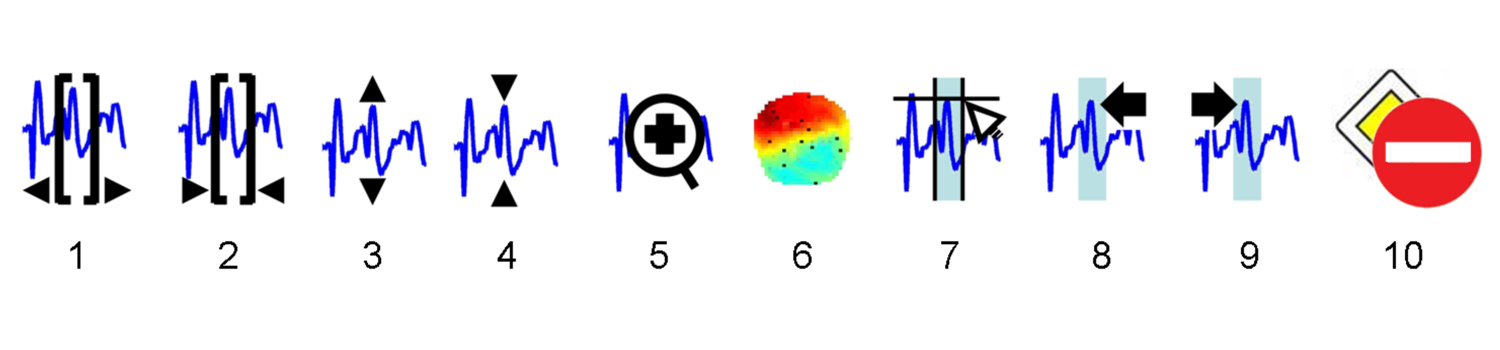
\includegraphics[width=100mm]{meeg/eeg_review_buttons}
\end{center}
\caption{\em SPM M/EEG \textsc{Review} buttons legend 1-2: increase/decrease width of plotted time window, 3-4: increase/decrease global scaling display factor, 5: zoom in, 7: add event, 8-9: scroll backward/forward data from marker to marker, 10: declare event as good/bad}
\end{figure}

\section{Batching and scripts}
Although all functions can be called by the GUI, using only the GUI for preprocessing multi-subject data is a cumbersome and error-prone affair. For this reason, we included functions in SPM8 which should make batching jobs feasible, with only a small amount of \matlab\ knowledge required. How would one batch a series of preprocessing steps in SPM8? There are two ways of doing this, the new batch system of SPM8, and generating scripts.

\subsection{The new SPM8 batch system}
This method uses the new SPM8 batch system described in chapter \ref{Chap:batch_interface}. Using this batch system, you can put together a series of processing steps by choosing options from menus, in any order you like. When the full ``job'' is specified which may be a sequence of several processing step, one executes the job.


\subsection{Script generation}
Another way of batching jobs is by using scripts, written in \matlab\ . In SPM8, you can generate these scripts automatically. To do this, you first have to analyze one data set using the GUI or batch system. In SPM8, whenever a preprocessing function is called, all the input arguments, once they have been assembled by the GUI, are stored in a ``history''. This history can then be used to not only see in detail which functions have been used on a data set, but also to generate a script that repeats the same analysis steps. The big difference is that, this time, no more GUI interactions are necessary because the script already has all the input arguments which you gave during the first run. The history of an \texttt{meeg} object can be accessed by \texttt{D.history}. 
\\
\\
To generate a script from the history of an SPM8 MEEG file, open the file in the M/EEG \textsc{Review} facility and select the \texttt{info} tab: a \texttt{history} tab is then available that will display all the history of the file. Clicking the \textsc{Save as script} button will ask for the filename of the \matlab\ script to save and the list of processing steps to save (default is all but it is possible to select only a subset of them). This will generate a script, which, when run, repeats the analysis. The script can also be obtained by directly calling the function \texttt{spm\_eeg\_history}.
\\
\\
Of course, this script can not only be used to repeat an analysis, but the script can also be seen as a template that can be re-used for other analyses. One needs minimal \matlab\ knowledge for these changes. For example, you can replace the filenames to preprocess a different subject. Or you can change parameters and then re-run the analysis. We have prepared an example, using the same example data set, as in the previous subsection to demonstrate this (see the file \texttt{man$\backslash$example\_scripts$\backslash$history\_subject1.m}). Note that these scripts can currently be used to do things that one couldn't do with the batch system. For example, if you want to exclude a channel from the analysis, there is no way to do this via the batch system. In the GUI, you would have to call display and switch the channel to 'bad'. With a script, you simply add a line like \texttt{D=badchannels(D, 23, 1)}, which flags channel 23 as bad (see also our example script after the filtering step). In summary, the idea is to preprocess a file through the GUI or batch system, then use the history-function to generate a template, and finally adapt this template to modify the analysis in some way. To run the example script on your computer, you need the data set that you can download from the SPM webpage (\footnote{\url{http://www.fil.ion.ucl.ac.uk/spm/data/eeg\_mmn/}}).

\chapter{3D source reconstruction: Imaging approach}
\label{ch:eeg_imaging}

Here is a brief help to the 3D reconstruction based on the Imaging approach. In the near future, this will be improved by including more theoretical details upon the different procedures as well as a practical tutorial that will guide the user through the SPM interface via the analysis of a sample dataset.

\section{Introduction}
\label{sec:imaginv_intro}
This chapter focuses on the imaging (or distributed) method for doing EEG/MEG source reconstruction in SPM.
Such an approach to spatial projection onto (3D) brain space consists in considering a large amount of dipolar sources all over the cortical sheet, with fixed locations and orientations. This renders the observation model linear, the unknown variables being the source amplitudes or power.\\
Given epoched and preprocessed data (see chapter ...), the evoked and/or induced activity for each dipolar source can be estimated, for a single time-sample or a wider peristimulus time window.\\
The obtained reconstructed activity is in 3D voxel space and enables mass-univariate analysis in SPM (see chapter...).

Contrary to PET/fMRI data reconstruction, EEG/MEG source reconstruction is a non trivial operation. Often compared to estimating a body shape from its shadow, inferring brain activity from scalp data is mathematically ill-posed and requires prior information such as anatomical, functional or mathematical constraints to isolate a unique and most probable solution~\cite{Baillet01}.

Distributed linear models have been around for more than a decade now~\cite{Dale93} and the proposed pipeline in SPM for 'Imaging' solution is classical and very similar to common approaches in the field. However, at least two aspects are quite original and should be emphasized here:
\begin{itemize}
\item Based on an empirical Bayesian formalism, the inversion is meant to be generic in the sense it can incorporate and estimate the relevance of multiple constraints of various nature; data-driven relevance estimation being made possible through Bayesian model comparison~\cite{peb1,Phillips05,Mattout06,karl_induced}.
\item The subject's specific anatomy is incorporated in the generative model of the data, in a fashion that eschews individual cortical surface extraction. The individual cortical mesh is obtained automatically from a canonical mesh in MNI space, providing a simple and efficient way of reporting results in stereotactic coordinates.
\end{itemize}

The EEG/MEG imaging pipeline is divided into four consecutive steps which characterize any inverse procedure. In this chapter, we go through each of those steps that all need to be completed when proceeding with a full inverse analysis:
\begin{enumerate}
	\item Source space modeling,
	\item Data co-registration,
	\item Forward computation,
	\item Inverse reconstruction.
\end{enumerate}

Whereas the three first steps are part of the whole generative model, the last step consists in the Bayesian inversion and is the only one involving the actual EEG/MEG data.\\

Everything which is described hereafter is a new feature in SPM and is accessible from SPM5 user-interface by choosing the 'EEG/MEG' application, '3D source reconstruction' and 'Imaging'.

\section{Data structure}
\label{sec:datastruct}
The Matlab structure describing a given EEG/MEG dataset in SPM is denoted as \textit{D}. Within that structure, each new inverse analysis will be described by a new cell of sub-structure field \textit{D.inv} and will be made of the following fields:

\begin{itemize}
	\item \textit{method}: character string indicating the method, either 'ECD' or 'Imaging' in present case;
	\item \textit{mesh}: sub-structure with relevant variables and filenames for source space and head modeling;
	\item \textit{datareg}: sub-structure with relevant variables and filenames for EEG/MEG data registration into MRI space;
	\item \textit{forward}: sub-structure with relevant variables and filenames for forward computation;
	\item \textit{inverse}: sub-structure with relevant variable, filenames as well as results files;
	\item \textit{comment}: character string provided by the user to characterize the present analysis;
	\item \textit{date}: date of the last modification made to this analysis.
\end{itemize}


\section{Source space modeling (\textit{mesh})}
The individual cortical mesh is obtained from a template mesh. Four Mesh sizes are available (3004, 4004, 5004 and 7204 vertices). If not yet obtained, the spatial normalization of the subject's T1 MRI into MNI space is performed (see \textit{spm\_preproc.m} based on tissue probability maps). The inverse of that transformation is computed and applied to the template mesh to furnish the individual cortical mesh.\\

Individual meshes for the inner-skull and scalp surfaces are also computed from the individual T1 MRI. They are obtained by performing a binary mask of the the volumes delimited by the inner-skull and scalp surface respectively. Then, using an initial spherical mesh, a realistic-shaped mesh is obtained for each of the two tissues and further regularized via an erosion and growing procedure.

The meshing module includes the following functions:
\begin{itemize}
	\item \textit{spm\_eeg\_inv\_mesh\_ui.m}: run the user interface for this module,
	\item \textit{spm\_eeg\_inv\_spatnorm.m}: normalize the T1 image if needed,
	\item \textit{spm\_eeg\_inv\_meshing.m}: main function to produce Cortex, Inner-skull and Scalp meshes,
	\item \textit{spm\_eeg\_inv\_getmasks.m}: produce masks of Inner-skull and Scalp,
	\item \textit{spm\_eeg\_inv\_ErodeGrow.m}: erosion and growing procedure,
	\item \textit{spm\_eeg\_inv\_getmeshes.m}: obtains the inner-skull and scalp meshes from correpsonding binary masks,
	\item \textit{spm\_eeg\_inv\_CtrBin.m}
	\item \textit{spm\_eeg\_inv\_TesBin.m}
	\item \textit{spm\_eeg\_inv\_ElastM.m}
	\item \textit{spm\_eeg\_inv\_checkmeshes.m}: displays the computed three meshes in the SPM main figure
\end{itemize}


\section{Data Registration (\textit{datareg})}
\label{sec:datareg}
There are two possible ways of coregistrating the EEG/MEG data into the structural MRI space.

\begin{enumerate}
	\item A Landmark based coregistration (using fiducials only).\\
	The rigid transformation matrices (Rotation and Translation) are computed such that they match each fiducial in the EEG/MEG space into the corresponding one in sMRI space. The same 					transformation is then applied to the sensor positions.
	\item Surface matching (between some headshape in MEG/EEG space and some sMRI derived scalp tesselation).
For EEG, the sensor locations can be used instead of the headshape. For MEG, the headshape is first coregistrated into sMRI space; the same transformation is then applied to the sensors.\\
Surface matching is performed using an Iterative Closest Point algorithm (ICP). The ICP algorithm~\cite{Besl_McKay} is an iterative alignment algorithm that works in three phases:
\begin{itemize}
	\item Establish correspondence between pairs of features in the two structures that are to be aligned based on proximity;
	\item Estimate the rigid transformation that best maps the first member of the pair onto the second;
	\item Apply that transformation to all features in the first structure. These three steps are then reapplied until convergence is concluded.
Although simple, the algorithm works quite effectively when given a good initial estimate.
\end{itemize}
\end{enumerate}

The data-registration module includes the following functions:
\begin{itemize}
	\item \textit{spm\_eeg\_inv\_datareg\_ui.m}: run the user interface for this module,
	\item \textit{spm\_eeg\_inv\_datareg.m}:	main co-registration function,
	\item \textit{spm\_eeg\_inv\_checkdatareg.m}: display meshes, sensor locations and fiducials in native MRI space to enable one checking the co-registration by eye.
\end{itemize}


\section{Forward computation (\textit{forward})}
Several methods are proposed, depending on the modality (EEG or MEG). All these approaches/functions are identical to the one initialy developed and provided by the BrainSTorm package (Matlab open-source and free software: http://neuroimage.usc.edu/brainstorm/).

For EEG~\cite{Ermer2001}:
\begin{enumerate}
	\item single sphere (scalp surface),
	\item three spheres (inner, outer skull and scalp surfaces),
	\item three spheres (+ Berg correction),
	\item overlapping spheres (one fitted sphere per sensor).
\end{enumerate}

For MEG~\cite{Huang1999}:
\begin{enumerate}
	\item single sphere,
	\item overlapping spheres
\end{enumerate}


The forward module includes the following functions:
\begin{enumerate}
	\item \textit{spm\_eeg\_inv\_forward\_ui.m}: run the user interface for this module,
	\item \textit{spm\_eeg\_inv\_BSTcreatefiles.m}:	create the structure and required files and parameters to interface SPM and BrainSTorm,
	\item \textit{spm\_eeg\_inv\_BSTfwdsol.m}:	compute the BrainSTorm forward solution, calling function \textit{bst\_headmodeler.m},
	\item \textit{spm\_eeg\_inv\_PCAgain}: compute the svd of the gain matrix.
\end{enumerate}


\section{Inverse reconstruction (\textit{inverse})}
The reconstruction is based on an empirical Bayesian approach to localize either the evoked response, the evoked power or the induced power, as measured by EEG or MEG.

The inverse module includes the following functions:
\begin{itemize}
	\item \textit{spm\_eeg\_inv\_inverse\_ui.m}: run the user interface for this module,
	\item \textit{spm\_eeg\_inv\_inverse.m}: main function,
	\item \textit{spm\_eeg\_inv\_evoked.m}:	compute the evoked response,
	\item \textit{spm\_eeg\_inv\_induced.m}:	compute the evoked and/or induced power,
	\item \textit{spm\_eeg\_inv\_msp.m}: Multivariate Source Prelocalisation~\cite{Mattout2005a}.
\end{itemize}
	

\chapter{M/EEG modelling and statistics}
\label{ch:eeg_stats}
After projection to 2D- or a 3D-space (source reconstruction), the
data is in voxel-space and ready to be analysed. There are several
ways how one can proceed. In this chapter, we will focus on analyzing
epoched time-series data. These can be event-related responses (ERPs),
event-related fields (ERFs) or single trials (M/EEG). 

In the following, we will go through the various stages of modelling
using typical examples to illustrate the procedures.

\section{Preliminary remarks}
All analyses can be done using either the graphical user interface
(GUI) or a batch system (i.e. using scripts in the SPM2-fashion,
s.~below). The GUI has the advantage that one doesn't need
matlab-knowledge to analyse data. The batch system has the
advantage that it is a fast and efficient way of entering model and
data. Its disadvantage is that some Matlab-Knowledge is
required. However, with this distribution, we provide some template
scripts to analyse (typical) data in batch mode. We assume that with slight
modifications these scripts can be used for most analyses.

\section{How epoched time-series are analysed in SPM}
After preprocessing the data (i.e.~epoching, filtering, etc...) and
projection to voxel-space, we have discretely sampled versions of
continuous fields \cite{kiebel_spm_eeg1}. These data can be analysed
with a mass-univariate approach using results from Random Field theory
(RFT) to adjust p-values for multiple comparisons \cite{kjw_hbf2}. The
model used at each voxel is a general linear model
\cite{kiebel_spm_eeg2}. Typically one wants to analyse
multiple subjects' data acquired under multiple conditions. Given that
each evoked-response has up to hundreds of time points, this is an
awful lot of data at each voxel. The ideal way to analyse these data
would be to specify a single hierarchical model (1st level: within-subject,
2nd level: over subjects) and estimate its parameters. However, this
is computationally not feasible because of the length of the data
vector at each voxel. Fortunately, such a 2-level model can usually be
split up into two models: The 1st level and the 2nd level model. The
input data to the 2nd model are contrasts of the 1st level model
\cite{kiebel_spm_eeg2}. In all cases considered in this chapter, this
2-stage procedure 
gives exactly the same results as the 2-level model. The reason for
this is that we are not really \textit{modelling} the data at the 1st
level, but simply forming weighted sums of the data, over time. For
example, if we are interested in the N170 component, one could average
the data from 150 to 190 milliseconds. This is exactly the approach
used in conventional ERP analysis. This approach is not a model,
because simply taking sums corresponds to using an identity matrix as
design matrix. This procedure leaves no degrees of freedom for error
estimation.\\

In summary, the SPM-approach is to form, at each voxel, weighted sums of
the data, over time, at the 1st level. We refer to these weighted sums
as contrast images. These form the input to the 2nd level, where
one usually tests for differences betwen conditions or between groups
(s.~below). The second level models are usually the same as the ones
one would use for functional magnetic resonance imaging (fMRI). Importantly,
these 2nd level models have enough degrees of freedom to estimate the
error, i.e.~statistics can be computed.\\

The output of such a 2nd level analysis is a
voxel-volume (or map), where each voxel contains one statistical
value. The associated p-value is adjusted for multiple
comparisons \cite{kjw_hbf2}. This adjustment is important, because there are many
other voxels or channels. One (disadvantageous) alternative to
adjustment is to consider only pre-selected channels or averages over
channels. This is why the adjustment is especially important for
high-density measurements, because there are many channels to
select from. We believe that it is generally too subjective
to select channels for analysis a-priori. We see the
GFT-adjustment as a good way of looking at the whole data without any
prior selection. This has been already demonstrated for EEG data (in
another context) by \cite{james_rft}.

\section{1st level}
At the 1st level, we select periods or time points in
peri-stimulus time that we would like to analyse. Critically, this
choice must be made a-priori by you. The alternative would be to not
treat peri-stimulus time as a factor, but as a dimension of a Random
Field approach. This alternative approach is often used in
time-frequency analysis of induced and evoked oscillations, where it
seems sometimes difficult to specifiy areas of interest on the
time-frequency plane a-priori \cite{james_rft}. 

In the present approach, time is a factor, and
you have to form weighted-sums over peri-stimulus time to provide
input to the 2nd level. Of course, you don't need to constrain
yourself to a single contrast around a specific peri-stimulus time,
but you can compute as many as you like. For example, to analyse
multiple aspects of an ERP, it is not uncommon to form averages around
several time-points of an ERP. At the 2nd level, these can be either
analysed independently or within one model to make inferences about
interactions between conditions and peri-stimulus time.

In the follwing, we will go through model specification and
computation of contrast images. This guide is not written as a
tutorial (i.e.~detailed instructions for a given data set), but
describes each design option and hopefully provides deeper background
knowledge.

\subsection{The aim}
The aim of the 1st level is to compute contrast images that provide
the input to the 2nd level. We will describe this using the example of
2D-data, i.e.~data that has not been source reconstructed but, for
each peri-stimulus time point, has been projected to a 2D-plane
(s.~chapter \ref{ch:eeg_source}).

\subsection{Start}
Start SPM by the command \textit{'spm eeg'} from the matlab command
line. Press the \textit{EEG/MEG} button. Your first choice is to
either specify the model design or the input data. One always starts
with the design. Currently, there are two design options: (i)
\textit{all options} and (ii) \textit{ERP/ERF}. The latter option is a
shortcut to quickly input an evoked responses study. We will first
describe \textit{all options} and then treat the \textit{ERP/ERF}
option as a special case.

\subsection{All options} 
You first have to answer the question whether
this is a 1st level design. This determines whether SPM expects to
model peri-stimulus time as a factor. Also, if one models first-level
data, SPM will ask next for \textbf{one} M/EEG-matfile before the
data was projected to voxel-space. The reason for this is that the voxel-images
lost important information during the conversion. For example, all timing
information were lost. With the nifti-images only, SPM doesn't
know the peri-stimulus time of each data point. However, this
information is critical as soon as you try to specify (later on)
linear weights in terms of peri-stimulus time. So, when you select an
M/EEG file, SPM will read timing information from this file. For an
ERP-study, the M/EEG-file of the average (ERP) is a good choice.

\subsection{How many factors?}
This question starts off the design specification proper. SPM needs to
know the number of factors which you want to model. At the 1st level,
there are typically only factors \textit{peri-stimulus time} and
\textit{condition}. If you like, you can further subdivide the
condition-factor in its components. For instance, if you have a 2x2
factorial design, you may want to specify 3 factors: \textit{factor1},
\textit{factor2} and  \textit{peri-stimulus time}. 

\subsection{Factor names and \# of levels for factors}
For each factor, you now input its name, e.g.~condition, and enter the
number of levels. For instance, if you have 2 conditions, you enter
2. For peri-stimulus time, you enter the number of time points in your
evoked responses. Important: You should call the peri-stimulus time
factor  'time'. For the number of levels for this special factor, SPM
defaults to the correct number of peri-stimulus time points. (Note
that it is currently not possible to model only a subset of time points.)

\subsection{Select design component}
You have the choice between \textit{Identity} and
\textit{Constant}. Your selected design components are combined (by
Kronecker tensor product) to form the 1st level design matrix. This
has also been described in \cite{kiebel_spm_eeg2}. For the 1st level,
you simply choose for all factors \textit{identity}. This completes
model specification.

\subsection{Data}
For selecting data, press the \textit{EEG/MEG} button again. After
selecting the \textit{SPM.mat} file, you are asked to select data for
each factor. The order in which you input data  depends on the order
of how you named the individual factors. We recommend that you make
the \textit{peri-stimulus time} factor the last factor. After
projection to voxel-space, the data are stored as 4-dimensional files
with the third dimension $z = 1$. If you want to input all
peri-stimulus time points for a given file, you have to select all
volumes along the 4th dimension. This is done by setting the number
'1' in the SPM-file selector (below the 'Filt' line) to '1:101', where
'101' is the total number of peri-stimulus time points. Of course, you
have to replace '101' by the number of time points of your
data (or by any natural number bigger than that). This choice will make
all time points selectable. Then right-click over the file 
names and \textit{Select all}. Press \textit{done} to confirm your
choice. This completes data selection.

\subsection{'Estimation'}
Although there is actually nothing to estimate, clicking the
\textit{Estimation} button will prepare some internal structure for
the results section. We kept this (otherwise redundant) estimation step to
provide for greater similiarity with other analyses using SPM.

\subsection{Results}
After clicking on \textit{Results}, choose the appropriate
\textit{SPM} and the contrast manager will pop up. In contrast to a usual
SPM study, we don't use the contrast manager to compute
statistics, but contrasts only!

Click \textit{Define new contrast...} and enter a name for your
contrast. Then note a (new) button called \textit{components} which is
only visible for M/EEG models. Clicking this button opens the contrast
components manager. This is simply a tool that exploits the knowledge
about the factors which you have specified earlier. Knowing the
factors and their levels makes it easy to split up a (long) contrast
weight vector into a few components. For each contrast weight vector,
each factor contributes one component. By using the Kronecker tensor
product, these components can be combined into the resulting contrast
weight vector. This is not only time-saving, but many people tend to
find this approach more intuitive than the usual approach of figuring
our the contrasts yourself. For instance, if you have specified
two conditions, you might be interested in their difference. Enter a
$[-1 \; \; 1]$ as contrast component. For the \textit{time} factor,
instead of entering one number for each time point, better click on 
the \textit{Generate} button. Click on the 'Time' button and specify
a rectangular averaging window by providing the start and end of this
window (in milliseconds). Press \textit{Compute}. You can see now in
the contrast manager window that your contrast weights have been
computed and are displayed above the identity (design)
matrix. You can also specify the contrast weights as usual in the
contrast box, but this would require to enter several hundreds to
thousands of numbers. Press \textit{ok} to proceed and compute the
contrast.

\subsection{Display}
You can display the resulting contrast image by using the
\textit{Display} button.

\subsection{ERP/ERF}
You can shortcut some of the question and especially the data
selection by choosing the \textit{ERP/ERF} option (instead of
\textit{all options} when specifying a design. This options assumes
that you have two factors, \textit{condition} and \textit{time}. There
are less questions during design specification. When selecting data,
you don't need to select all time point, but only the first! SPM will
assume that you want to select all time points of the selected
file. Using this option will otherwise result in the same model
as described above.

\subsection{Multiple subjects}
For each of your subjects, you perform these operations in a separate
1st-level analysis. For each subject, you want to compute the same
contrasts and use them as input to a model, where subjects is the
repetition factor. 

\section{2nd level models}
For 2nd level modelling, you can use different ways to specify a
model. There is \textit{Basic models} which was primarily developed for
PET/fMRI but is equally appropriate for EEG/MEG data. These are
suited best when the model is simple (like a 1-sample or 2-sample
t-test). In our experience, most EEG/MEG models fall into this
category of simple models. If models are more complicated, like, e.g.,
two groups with multiple subjects/conditions, we recommend using the
\textit{EEG/MEG} models.

\subsection{All options}
As above, go for \textit{All options}. This time, press 'no' for the
question 'Is this a first-level design'. 

\subsection{Factors}
This includes all factors, even repetition factors. For example, at
the 2nd level a 2x2 factorial design has 3 factors: \textit{subject},
\textit{factor1} and \textit{factor2}.
 
\subsection{Design partitions and design components}
The way this modelling device constructs a design matrix is by using the
Kronecker tensor product on the hierarchy of specified design
components. However, some/many designs can't be constructed in this
way. For example, the design matrix of a paired two sample-test
consists of two merged partitions, each of which is a Kronecker tensor
product of design components. For each partition, the factors and the
levels are the same. The difference is in the choice of the design
components for each factor under each partition. For example, for a
paired two-sample-test, one has 2 factors (subjects and conditions)
and 2 design partitions. For the 1st partition, choose
\textit{Constant} for subjects and \textit{Identity} for
conditions. For the 2nd partition, it's the other way around,
i.e.~\textit{Identity} for subjects and \textit{Constant} for
conditions.

\subsection{Covariance components}
Specification of the covariance components determines the error
model \cite{daniel_hbf2}. For each factor, there are two questions:
(i) Identical variance for
factor $xxx$, and (ii) Independence for factor $xxx$. SPM constructs all the
variance components from your answers. The first question pertains to
the assumption whether each level of this factor has identical
variance. The second questions asks whether the different levels for a
given factor are correlated. Some examples: For a repetition factor
like subjects, you should always answer both questions with yes. For a
group factor, one would assume that the levels of this factor (the
groups) have unequal variance structures, but are uncorrelated (i.e.,
(i) no, (ii) yes). For a condition factor, the choice is up to
you. A very restrained model would follow from using (i) yes (ii)
yes, whereas the most liberal model is given by (i) no (ii) no. 

\subsection{Data}
For each combination of factors, SPM asks you for the filenames of the
data. Sometimes, this process can be more convient for you, when you
have specified the factors in a specific order. For example, if you
have two factors \textit{subjects} and \textit{condition}, the order
(i) subjects, (ii) condition will ask for all images for each
subject. This is convienient if you have stored the contrast images
in their individual subject folder. This is the case, if you
have computed 1st level contrasts following the approach described
above. However, if, in an intermediate step, you have saved contrasts
in condition-specific folders, the alternative order ((i) condition, (ii)
subjects) is more appropriate.

\subsection{Estimation and Results}
The estimation follows the usual scheme, i.e.~for a classical
estimation procedure we use exactly the same routine as for PET/fMRI
data (i.e.~maximum-likelihood estimators for the parameters and Restricted 
Maximum Likelihood for estimation of the variance parameters).

For specification of contrasts, you have the option to specify
contrasts component-wise. This can be useful for complex designs, when
it's no longer easy to work out the interaction contrasts.

For 2D data the statistical map is displayed instead of the usual
glass brain. You can invoke all the usual functions that are also
available for fMRI/PET data. An additional option is \textit{channels}
which let you visualise to which voxel each channel maps. You can
select this option by right-clicking the button on the statistical 
map background. SPM asks you then for one of the original M/EEG-mat
files to read the channel mapping.


\chapter{Equivalent current Dipole fitting}
\label{ch:eeg_ecd}

This little chapter demonstrates how to use the ECD (Equivalent Current Dipole) routines with the multimodal dataset available on the FIL website. The aim is to fit a single dipole on the N170 wave visible in the 3 conditions.
I will briefly describe how to analyse the dataset. For more details about the implementation, please refer to the help bit of and comments in the routines themselves.

\section{Necessary data}
Before proceeding any further, we have to make sure that we have all the necessary data in the right format
We need 
\begin{itemize}
\item the {\it amri.img/hdr} structural MRI of the subject. It will be used to build the head model and display the results in the subject's anatomical space.\\
\item the {\it mae\_eeg.dat/mat} EEG data files. These are the fully processed data with one ERP per condition.
\item the coordinates of the sensors, fiducial markers and scalp points (headshape) in 3 distinct {\it *.mat} files.
\end{itemize}

In the dataset provided on the web, the raw {\it *.pol} files are available. It is necessary to prepare these files to use them with the source reconstruction routines. This is a crucial step as the registration between the "EEG space" and "patient/image space" relies entirely on these files! 
To prepare these files, use the little script {\it create\_fid\_files.m} distributed with SPM5. A copy is also available at the end of this chapter.

Once we have all the files ready, we can proceed with the 3 main steps: building the model, fitting the dipole and displaying the results. To launch the GUI, press "3D source reconstruction" in the main window of SPM.

\section{Model building}
After selecting the data file {\it mae\_eeg.mat} and the method "ECD", the first step is building the meshes for the scalp and inner skull volume. This is done automatically through the "Meshes" button. Select the structural MRI to use ({\it amri.img} here) and wait...

This step takes some time as the MRI is normalised and segmented. The normalisation parameters are saved in the {\it amri\_vbm\_inv\_sn.mat} file and will be used later to map coordinates between the template and subject spaces. With the segmentation, the brain and scalp binary volumes are built ({\it amri\_iskull.img} and {\it amri\_oscalp.img} ). These are used to build the outer scalp and inner skull surface meshes. These are saved in the {\it model\_head\_amri.mat} file with other information. The scalp mesh is also saved in the file {\it amri\_scVert.mat}.

Once the head model is ready, we can co-register the EEG space with subject/image space. Use the "Data Reg." button and decide if the registration should be based on the fiducials only (which is quite approximate) or the fiducials and the scalp surface (which should be more precise). Then select the appropriate files: {\it fid\_eeg.mat}, {\it fid\_MRI.mat}, {\it headshape\_orig.mat}, {\it amri\_scVert.mat} and let the routine work.

To prepare the model for the forward solution, simply press "ForwardComp." and "individual" to use the subject's own MRI. The forward model uses a spherical approximation. The best fitting sphere are adjusted on the scalp surface and 2 other spheres are added to model the scalp and skull outer surfaces. Obviously the head is not spherical and there will be a mismatch between the scalp/brain surfaces and their respective spheres. We have used the idea proposed by Spinelli et al., 2000 \cite{Spinelli2000}, where the brain volume is warped into a sphere. This allows us to use an analytical formula to calculate the forward solution for each dipole location while preserving some anatomical characteristics: superficial (resp. deep) sources remain superficial (resp. deep) in the spherical head model.

At this last step, the electrodes are also introduced in the head
model and positioned relative to the subject head, as in the MRI. The
{\it model\_head\_amri.m} at contains the information about the fitted spheres and electrodes. Dipole fitting of the data is now possible.

\section{Dipole fitting}
By pressing the "Inverse Sol." you launch the dipole fitting procedure. A number of questions have to be answered in order to specify the kind of solution you want:
\begin{itemize}
\item "Condition to use", select which condition is used to fit the dipole(s). So far, it is not possible to fit multiple conditions (or linear combinations of them) at the same time. For example, for differences between conditions, you should pre-calculate this difference before trying to fit ECDs. \\
\item "Time window", define the time window in ms on which the ECDs should be fitted. With the N170 demo data, a good window is 150 to 180.\\
\item "Number of dipoles", this is the crucial questions. How many dipoles should be used? It's up to you to decide... With the demo data, from the look of the EEG scalp map, 1 ECD should be enough.\\
\item "Number of random seeds". In order to avoid being trapped in a local minimum during the optimisation process because of a peculiar starting point. The algorithm can be launched from multiple random starting 'seeds'. If they all converge to approximately the same solution, then we'll have most surely reached the local optimum.\\
\item "Orientation of the dipoles". The location of the ECD will be constant throughout the time window but its orientation can be left free or be fixed as well. Leaving the orientation free allows the dipoles to rotate over time. To fix the orientation, we can use the (weighted according to the EEG power)) mean over the time window or use the orientation of the ECD fitting the time instant with maximum EEG power.\\
\item "File name". File names are suggested but feel free to change it!
\end{itemize}

After fitting the N random seeds, the routine tries to group them in clusters of similar ECDs according to their location and signal variance explained. Eventually, these 'grouped' ECDs are displayed on the subject anatomy. The result of this clustering is saved in a mat file starting by {\it res\_} and finishing with the name you entered.

\section{Result display}

Results can be redisplayed with the routine {\it spm\_eeg\_inv\_ecd\_DrawDip.m}. The routine asks you to select the solution file you want to display and the MR image to be used.

\section{Preparing the *.pol files}
\begin{quote}
% Just quick and dirty programming to extract the information from the .pol
% files: fiducials, sensors & headshape in EEG space.
 
% Actually, I just opened the ascii files and copy the coord of the EEG 
% fiducials here... Much easier.
 
% Order of the fiducials is: LE, RE, Na
fid\_eeg = ([-0.0587687  6.79448 -0.00636311 ; ...
            0.0352661   -6.78906    -0.00369206 ; ...
            9.3675  0.0260009   0.00481311] + ...
           [-0.0328487  6.78991 0.00636288 ; ...
            0.0563513   -6.79533    0.00369206 ; ...
            9.45206 -0.0260009  -0.00481297])/2 ...
            * 10 ; % To convert cm into mm
 
% These are coordinates picked by hand on the sMRI.
% So it's quite an approximation of where the fiducials are really...
fid\_mri = [-71.8 3.5 -58.8 ; ...
            71.3 -6  -62.5 ; ...
            0   90.6 -28.4]        ;
            
% I edited the .pol files to REMOVE the first few lines with
% fiducial information.
sensors = load('sensors\_noFid.pol','-ASCII')*10;
headshape = load('headshape\_noFid.pol','-ASCII')*10;
    % Again, multiply by 10 to get the measures in mm instead of cm
 
% ATTENTION !!!
% Polhemus, uses the axes in a different orientation!
% It's still a right handed system but axes are:
% - x: from back to front (versus left to right)
% - y: from right to left (versus back to front)
% - z: from bottom to top
%
% To make coord systems compatible, it is necessary to rotate clockwise the
% coord by 90 degree around the z axis.
 
Rot = spm\_matrix([0 0 0 0 0 -pi/2]); Rot = Rot(1:3,1:3);
fid\_eeg = (Rot*fid\_eeg')';
sensors = (Rot*sensors')';
headshape = (Rot*headshape')';
 
save fid\_eeg fid\_eeg
save fid\_mri fid\_mri
save sensors\_orig sensors
save headshape\_orig headshape

\end{quote}

%%%%%%%%%%%%%%%%%%%%%%%%%%%%%%%%%%%%%%%%%%%%%%%%


\chapter{Dynamic Causal Modelling for M/EEG \label{Chap:eeg:DCM}}

\section{Introduction}
Dynamic Causal Modelling (DCM) is based on an idea initially developed for fMRI
data: The measured data are explained by a network model consisting of
a few sources, which are interacting dynamically. This network model
is inverted using a Bayesian approach, and one can make inference
about interesting parameters like connection strength between sources,
or the modulation of connection strengths by task. For M/EEG data, DCM
is a powerful technique for inferring about parameters that one
doesn't observe with M/EEG directly. Instead of asking 'How does the
source strength of the source in left superior temporal gyrus change
between condition A and B?', one can ask questions like 'How does the feedback
connection from this left STF source to left primary auditory cortex
change between condition A and B?'. In other words, one isn't limited
to questions about source strength as estimated using a source
reconstruction approach, but can test hypotheses about what is
happening between sources, in a network. In M/EEG, this analysis
approach is probably very potent because M/EEG data is highly resolved
in time, and the inference is not, like in fMRI, about rather
phenomenological variables, but about neurobiologically plausible
parameters which relate more directly to the causes of the underlying 
neuronal dynamics. However, it's still early days for DCM for
M/EEG. The key methods paper appeared in 2006, and the
first DCM studies about the mismatch negativity phenomenon only came out
in 2007/2008. Although DCM for M/EEG is a novel technique that still
has to show its full potential in applications, we believe that DCM is
just the right approach to get at the interesting bits in M/EEG
data: At its heart DCM is a source reconstruction technique and for
the spatial domain we use exactly the same leadfields as other
approaches. However, what makes DCM so interesting, is to combine the
spatial forward model with a temporal forward model, e.g., the
connectivity between sources. This critical ingredient not only makes
the source reconstruction more robust by implicitly constraining the
spatial parameters, but also allows one to infer about connectivity.
\\
\\
A number of people in our methods group are working on further
improvements and extensions to DCM. At the same time, we take great
care that the core functionality implemented in SPM8 is robust and
well usable. In the following, we will describe the usage of DCM for evoked
responses (both MEG and EEG), DCM for induced responses (i.e., based
on power data in the time-frequency domain), and DCM for local field
potentials (measured as steady-state responses). All three DCMs share the
same interface, because many of the questions that DCM needs to
ask to analyse some data are the same. Therefore, we will first
describe DCM for evoked responses, and then point out where the
differences to the other two DCMs lie.
\\
\\
Note that this manual is only a rough guide to DCM for
M/EEG. If you want to read more about the scientific background, the
algorithms used, or how one would typically use DCM in applications,
we recommend reading a fair dosage of our papers. The two key methods
contributions can be found in \cite{od_dcm_erp} and
\cite{sjk_dcm_erp}. Two other contributions using the model for
testing interesting hypotheses about neuronal dynamics are described 
in \cite{sjk_dcm_intrinsic} and \cite{matthias_dcm_constraints}. At
the time of writing, there were also three application papers published which demonstrate
what kind of hypotheses can be tested with DCM
\cite{mg_dcm_repro,mg_feedback,marta_mmndcm}. Another good source of
background information is the recent SPM book
\cite{spm_book}, where Parts 6 and 7 cover not only DCM for M/EEG but
also related research from our group. The DCMs for induced responses
and steady-state responses are covered in \cite{cc_induced} and
\cite{rm_spectralnmm,rm_massmodelspectral}. Also note that there is a DCM example file, which we put onto the webpage http://www.fil.ion.ucl.ac.uk/spm/data/eeg\_mmn/. After downloading DCMexample.mat, you can load (see below) this file using the DCM GUI, and have a look at the various options, or change some, after reading the description below.

\section{Overview}
In summary, the goal of DCM is to explain measured data (like evoked
responses) as the output of an interacting network consisting of a few
areas that receive input (i.e., the stimulus). The differences between
evoked responses, measured under different conditions, are modelled as
a modulation of selected DCM parameters, e.g. cortico-cortical
connections \cite{od_dcm_erp}. This interpretation of the evoked
response makes hypotheses about connectivity directly testable. For 
example, one can ask, whether the difference between two
evoked responses can be explained by some top-down modulation of early areas
\cite{mg_dcm_repro}. Importantly, because model inversion is done
using a Bayesian approach, one can also compute Bayesian model evidences. These
can be used to compare alternative, equally plausible, models and
decide which model is the best \cite{stefan_neurodynamics}. 

DCM for evoked responses takes the spatial forward model into
account. This makes DCM a spatiotemporal model of the full data set
(over channels and peri-stimulus time). Alternatively, one can
describe DCM also as a spatiotemporal source reconstruction algorithm which uses
additional temporal constraints given by neural mass dynamics and
long-range effective connectivity. This is achieved by parameterising
the lead-field, i.e.,~the spatial projection of source 
activity to the sensors. In the current version, this can be done
using two different approaches. The first assumes that the leadfield
of each source is modelled by a single equivalent current dipole 
(ECD) \cite{sjk_dcm_erp}. The second approach posits that each source
can be presented as a 'patch' of dipoles on the grey matter sheet
(Daunizeau et al., in preparation). This spatial model is complemented
by a model of the temporal dynamics of each source. Importantly, these
dynamics not only describe how the intrinsic source dynamics evolve
over time, but also how a source reacts to external input, coming
either from subcortical areas (stimulus), or from other cortical
sources.

The GUI allows to enter all information necessary to specify a
spatiotemporal model for some data. If you want to analyze lots of
models, we recommend using a batch script. An example of such 
a script (\textit{DCM\_ERP\_example}), which can be adapted to your
own data, can be found in the \textit{man/example\_scripts/} folder of
the distribution. You can run this script on some example data provided by via the SPM webpage (http://www.fil.ion.ucl.ac.uk/spm/data/eeg\_mmn/). However, you first have to preprocess these data to produce an evoked response by going through the preprocessing tutorial (chapter \ref{ch:eeg_tutorial}) or by running the histexample.m scipt in the example\_scripts folder.

\section{Calling DCM for ERP/ERF}
After calling \textit{spm eeg}, you see SPM's graphical user interface,
the top-left window. The button for calling the DCM-GUI is found
in the second partition from the top, on the right hand side. When
pressing the button, the GUI pops up. The GUI is partitioned into five 
parts, going from the top to the bottom. The first part is about
loading and saving existing DCMs, and selecting the type of model. The second part is about selecting
data, the third is for specification of the spatial forward model, the
fourth is for specifying the connectivity model, and the last row of
buttons allows you to estimate parameters and view results.

You have to select the data first and specify the model in
a fixed order (data selection $>$ spatial model $>$
connectivity model). This order is necessary, because there are
dependencies among the three parts that would be hard to resolve
if the input could be entered in any order. At any time, you can switch forth and back from one part to
the next. Also, within each part, you can specify information in any
order you like.  

\section{load, save, select model type}
At the top of the GUI, you can load an existing DCMs or save the one
you are currently working on. In general, you can \textit{save} and
\textit{load} during model specification at any time. You can also
switch between different DCM analyses (the left menu). The default is 'ERP' which is DCM
for evoked responses described here. Currently, the other two typs are are steady-state responses
(SSR) and induced responses (IND); both are also described in this
manual. The menu on the right-hand side lets you choose the neuronal model. Currently, there are four model types. The first is 'ERP', which is the standard model described in most of our papers, e.g.~\cite{od_dcm_erp}. The second is 'SEP', which uses a variant of this model, however, the dynamics tend to be faster \cite{andre_sigmoid}. The third is 'NMM', which is a nonlinear neural mass model based on a first-order approximation, and the fourth is 'MFM', which is also nonlinear and is based on a second-order approximation. The latter two options haven't been described in the literatue yet, but are under review.

\section{Data and design}
In this part, you select the data and model between-trial
effects. The data can be either event-related 
potentials or fields. These data must be in the SPM-format. On the
right-hand side you can enter trial indices of the evoked responses in
this SPM-file. For example, if you want to model the
second and third evoked response contained within an SPM-file, specify
indices 2 and 3. If the two evoked responses, for some reason, are in
different files, you have to merge these files first. You can do this
with the SPM preprocessing function \textit{merge}
(\textit{spm\_eeg\_merge}), s.~chapter
\ref{Chap:eeg:preprocessing}. You can also choose how you want to
model multiple evoked responses. When you enter multiple evoked
responses, the default is to model the modulations of connectivity
parameters independently of each other. You can change this default to
model the way connection weights are modelled over trials. For
example, when you want to model three evoked responses, you can model
the modulations of a connection strength of the second and third
evoked responses as two uncoupled multiplicative gains on the connection
strength of the first evoked response. However, you can also choose to
couple the connection strength of the first evoked response with the
two gains by imposing a linear relationship on how this connection
weight changes over trials. This can be useful when one wants to add
constraints on how connection strength (or other DCM parameters)
change over trials. A compelling example of this technique can be
found in \cite{marta_mmndcm}.

When you hit enter after entering the
row vector of trial indices, a file requester will ask you for the
name of the SPM-file. Alternatively, you can also press the button
'data file'. Under 'time window (ms)' you have to enter the
peri-stimulus times which you want to model, e.g. 1 to 200 ms. 

You can choose whether you want to model the mean or
drifts of the data at sensor level. If you don't want any such terms,
select 0 for 'detrend', otherwise select the number of discrete cosine
transform terms you want to use to model the mean (1) or low-frequency
drifts ($> 1$). In DCM, we use a projection of the data to some
subspace to reduce the amount of data. The type of spatial projection
is described in \cite{matthias_dcm_constraints}. You can select the
number of (first) modes you want to keep. The default is 8.

You can also choose to window your data, along peri-stimulus time,
with a hanning window (radio button). This windowing will reduce the
influence of the beginning and end of the time-series. 

If you are happy with your data selection, the projection and the detrending
terms, you can click on the $>$ (forward) button, which will bring you to
the next stage \textit{electromagnetic model}. From this part, you can
press the red $<$ button to get back to the data and design part.

\section{Electromagnetic model}
With the present version of DCM, you have three options how to spatially
model your evoked responses. Either you use a single equivalent
current dipole (ECD) for each source, or you use a patch on the
cortical surface as source model (IMG), or you don't use a spatial model at all (local field potentials (LFP)). The second option is not
described in the peer-reviewed literature yet (Daunizeau et al., in
preparation). In all three cases, you have to enter the source names (one
name in one row). For ECD and IMG, you have to specify the prior source locations (in mm in MNI
coordinates). Note that DCM uses by default uninformative priors on  
dipole orientations, but tight priors on locations. This is because tight priors on locations ensure that the posterior location will not deviate to much from its prior location. This means each dipole stays in its designated area and retains its meaning. The prior location for each
dipole can be found either by using available anatomical knowledge or
by relying on source reconstruction of comparable studies. Also note
that the prior location doesn't need to be overly exact, because the
spatial resolution of M/EEG is on a scale of several millimeters. 
You can also load the prior locations from a file
('load'). You can visualize the locations of all sources when you
press 'dipoles'. The onset-parameter determines when the stimulus,
presented at 0ms peri-stimulus time, is assumed to cause an
impulse. In DCM, we usually do not model the quite small responses of
early potentials, but start modelling at the first large
deflection. Because the propagation of the stimulus impulse throught
the input nodes causes a delay, we found that the default value of 60
ms onset time is a good value for many evoked responses where the
first large deflection is seen around 100 ms. However, this value is a
prior, i.e., the inversion routine can adjust it. The prior mean should be chosen according to the specific responses of interest because the time until the first large deflection appears are dependent on your paradigm or the modality you are working in, e.g. audition or vision. 
You may also find that changing the onset prior has some effect on how your data are
fitted. This is because the onset time has strongly nonlinear effects
(a delay) on the data, which might cause differences in which maximum
was found at convergence, for different prior values. 

When you want to proceed to the next model 
specification stage, hit the $>$ (forward) button and proceed
to the \textit{neuronal model}.

\section{Neuronal model}
There are five (or more) matrices which you need to specify by button presses. The
first three are the connection strength parameters for the first
evoked response. There are three types of connections,
\textit{forward}, \textit{backward} and \textit{lateral}. In each of 
these matrices you specify a connection \textit{from} a source area
\textit{to} a target area. For example, switching on the element
$(2,\;1)$ in the intrinsic forward connectivity matrix means that you
specify a forward connection from area 1 to 2. Some people find the
meaning of each element slightly counter-intuitive, because the
column index corresponds to the source area, and the row index to the
target area. 

In the present GUI implementation, there is only one input
allowed. This input can go to any and multiple areas. You can select
these receiving areas by selecting area indices in the \textit{C input} vector.

The \textit{B} matrix contains all gain modulations of connection
strengths as set in the $A$-matrices. These modulations model the
difference between the first and the other modelled evoked
responses. For example, for two evoked responses, DCM explains the
first response by using the $A$-matrix only. The 2nd response is
modelled by modulating these connections by the weights in
the $B$-matrix.

\section{Estimation}
When you are done with model specification, you can hit the
\textit{estimate} button in the lower left corner. If this is the
first estimation and you have not tried any other source
reconstruction with this file, DCM will build a spatial forward
model. You can use the template head model for quick results. For
this, you answer 'no' to the question 'Redefine MRI fiducials?', and
'yes' to 'Use headshape points?' DCM will now
estimate model parameters. You can follow the estimation process by
observing the model fit in the output window. In the matlab command
window, you will see each iteration printed out with
expected-maximization iteration number,free energy $F$, and the
predicted and actual change of $F$ following each iteration
step. At convergence, DCM saves the results in a DCM file, by default
named 'DCM\_ERP.mat'. You can save to a different name, for example
because you want to estimate multiple models, by pressing 'save' at
the top of the GUI and write to a different name. 

\section{Results} 
After estimation finished, you can assess the results
by choosing from the pull-down menu at the bottom (middle). 

With \textit{ERPs (mode)} you can plot, for each mode, the data for
both evoked responses, and its fit by the model. 

When you select \textit{ERPs (sources)}, the dynamics of each area are
plotted. The activity of the pyramidal cells (which is the
reconstructed source activity) are plotted in solid
lines, and the activity of the two interneuron populations are plotted
as dotted lines.

The option \textit{coupling (A)} will take you to a summary about the
posterior distributions of the connections in the $A$-matrix. In the
upper row, you see the posterior means for all intrinsic
connectivities. As above, element $(i,\; j)$ corresponds to a
connection from area $j$ to $i$. In the lower row, you'll find, for
each connection, the probability that its posterior mean is different
from the prior mean, taking into account the posterior variance.

With the option \textit{coupling(B)} you can access the posterior
means for the gain modulations of the intrinsic connectivities and
their probability that they are unequal the prior means.

With \textit{coupling(C)} you see a summary of the posterior
distribution for the strength of the input into the input receiving
area. On the left hand side, DCM plots the posterior means for each
area. On the right hand side, you can see the corresponding
probabilities (s.~above).


The option \textit{Input} shows you the estimated input function. As
described by \cite{od_dcm_erp}, this is a gamma function with an
addition of some low-frequency terms.

With \textit{Response}, you can plot the selected data, i.e.~the data,
selected by the spatial modes, but back-projected into sensor space.

With \textit{Response (image)}, you see the same as under Results but
plotted as an image in grey-scales.

And finally, with the option \textit{Dipoles}, DCM displays an
overlay of each dipole on an MRI template using the posterior means of
its 3 orientation and 3 location parameters. This makes sense only if
you have selected an ECD model under \textit{electromagnetic model}.

Before estimation, when you press the button 'Initialise' you can
assign parameter values as initial starting points for the free-energy
gradient ascent scheme. These values are taken from another already
estimated DCM, which you have to select. 

The button \textit{BMC} allows you do Bayesian model comparison of
multiple models. After selecting DCMs, you will see, at the top, a
bar plot of the log-model evidences for all models. At the bottom, you
will see the probability, for each model, that it produced the
data. By convention, a model can be said to be the best among a
selection of other models, with strong evidence, if its log-model
evidence exceeds all other log-model evidences by at least 3. 

\section{Steady-State Responses}

\subsection{Model specification}
DCM for steady state responses can be applied to M/EEG or intracranial data. 

The data must first be prepared using the temporal pre-processing option; 'other', then 'prep'. Here you specify the data type (MEG, EEG or LFP), and select the channels for a DCM analysis. In general you select all MEG/EEG channels and all or a subgroup of LFP channels from the areas you are interested in modelling as a network. A sample script to convert raw txt data, called textit{spm\_lfp\_txt2mat} can be found in the toolbox folder.

The top panel of the DCM for ERP window allows you to toggle through available analysis methods. On the top left drop-down menu, select 'SSR'. The second drop-down menu in the right of the top-panel allows you to specify whether the analysis should be performed using a model which is linear in the states, for this you can choose ERP. Alternatively you may use a conductance based model, which is non-linear in the states by choosing, 'NMM' or 'MFM'. (see \cite{andre_sigmoid} for a description of their differences).
 
The steady state (frequency) response is generated automatically from the time domain recordings. The time duration of the frequency response is entered in the second panel in the time-window.  The options for detrending remove either 1st, 2nd, 3rd or 4th order polynomial drifts from channels data. In the subsampling option you may choose to downsample the data before constructing the frequency response. The number of modes specifies how many components are from the leadfield are present in channel data. The between trial effects and design matrix entry follow as above in the case of ERPs.

\subsection{The Lead-Field}
The cross-spectral density is a description of the dependencies among the observed outputs of these neuronal sources. To achieve this frequency domain description we must first specify the likely sources and their location. If LFP data are used then only source names are required. This information is added in the third panel by selecting 'LFP'. Alternatively, x,y,z coordinates are specified for ECD or IMG solutions. 


\subsection{Connections}
The bottom panel then allows you to specify the connections between sources and whether these sources can change from trial type to trial type. 

On the first row, three connection types may be specified between the areas. For NMM and MFM options these are Excitatory, Inhibitory or Mixed excitatory and inhibitory connections When using the ERP option the user will specify if connections are 'Forward', 'Backward' or 'Lateral' To specify a connection, switch on the particular connection matrix entry. For example to specify an Inhibitory connection from source 3 to source 1, turn on the 'Inhib' entry at position (3,1).

On this row the inputs are also specified. These are where external experimental inputs enter the network.

The matrix on the next row allows the user to select which of the connections specified above can change across trial types. For example in a network of two sources with two mixed connections (1,2) and (2,1), you may wish to allow only one of these to change depending on experimental context. In this case, if you wanted the mixed connection from source 2 to source 2 to change depending on trial type, then select entry (2,1) in this final connection matrix.


\subsection{Cross Spectral Densities}
The final selection concerns what frequencies you wish to model. These could be part of a broad frequency range e.g. like the default 4 - 48 Hz, or you could enter a narrow band e.g. 8 and 12 Hz, will model the alpha band in 1Hz increments.

Once you hit the 'invert DCM' option the cross spectral densities are computed automatically (using the spectral-toolbox). The data for inversion includes the auto-spectra and cross-spetra between channels or between channel modes. This is computed using a multivariate autoregressive model, which can accurately measure periodicities in the time-domain data. Overall the spectra are then presented as an upper-triangular, s x s matrix, with auto-spectra on the main diagonal and cross-spectra in the off-diagonal terms.

\subsection{Output and Results}
The results menu provides several data estimates. By examining the 'data', you will be able to see observed spectra in the matrix format mentioned above. Selecting 'Cross-spectral density' gives both observed and predicted responses. To examine the connectivity estimates you can select the 'coupling (A)' results option, or for the modulatory parameters, the 'coupling (B)' option. Also you can examine the input strength at each source by selecting the 'coupling (C)' option, as in DCM for ERPs. The option 'trial-specific effects' shows the change in connectivity parameter estimates (from B) from trial to trial relative to the baseline connection (from A). To examine the spectral input to these sources choose the 'Input' option; this should look like a mixture of white and pink noise. Finally the 'dipoles' option allows visualisation of the a posteriori position and orientation of all dipoles in your model. 


\section{Induced responses}
DCM for induced responses aims to model coupling within and between frequencies that are associated with linear and non-linear mechanisms respectively. The procedure to do this is similar to that for DCM for ERP/ERF. In the following, we will just point out the differences of how to specify models in the GUI. Before using the technique, we recommend reading about the principle behind DCM for induced responses to get an intuition for this novel technique \cite{cc_induced}.

\subsection{Data}
The data to be modelled must be single trial, epoched data. We will model the entire spectra, including both the evoked (phase-locked to the stimulus) and induced (non-phase-locked to the stimulus) components. 

\subsection{Electromagnetic model}
Currently, DCM for induced responses uses only the ECD method to capture the data features. Note that a difference to DCM for evoked responses is that the parameters of the spatial model are not optimized. This means that DCM for induced responses will project the data into source space using the spatial locations provided by you. 


\subsection{Neuronal model}
This is where you specify the connection architecture. Note that in DCM for induced responses, the $A$-matrix encodes the linear and nonlinear coupling strength between sources.


\subsection{Wavelet transform}
This function can be called below the connectivity buttons and allows one to transfer data into the time-frequency domain using a Morlet Wavelet transform as part of the feature extraction.  There are two parameters: The frequency window defines the desired frequency band and the wavelet number specifies the temporal-frequency resolution. We recommend values greater than 5 to obtain a stable estimation.

\subsection{Results}

\subsubsection{Frequency modes}
This will display the frequency modes, identified using singular value decomposition of spectral dynamics in source space (over time and sources).

\subsubsection{Time-Frequency}
This will display the observed time-frequency power data for all pre-specified sources (upper panel) and the fitted data (lower panel).

\subsubsection{Coupling (A-Hz)}
This will display the coupling matrices representing the coupling strength from source to target frequencies.


%%%%%% UTILITIES %%%%%%

\part{Utilities}

\include{disp}
\include{checkreg}
\include{imcalc}
%\include{spm_surf}
\include{dicom}
\include{minc}
\include{ecat}
%\include{runbatch}
%\include{cdir}
%\include{md}
\include{defs}
%\include{ui}

%%%%%% TOOLS %%%%%%

\part{Tools}
\include{hdw}
\include{dartel}
\chapter{FieldMap Toolbox \label{Chap:FieldMap}}

\section{Introduction}

This chapter describes how to use the FieldMap toolbox version 2.1\footnote{
FieldMap Version 2.0 can be downloaded as part SPM5:
\url{http://www.fil.ion.ucl.ac.uk/spm/software/spm5/}\\
FieldMap Version 1.1 for SPM2 can be downloaded from
\url{http://www.fil.ion.ucl.ac.uk/spm/toolbox/fieldmap/}}
 for creating unwrapped field maps that can be used to do geometric distortion correction of EPI images \cite{chloe_distortion,chloe_distortion2,ja_geometric}. The toolbox uses methods based on earlier work by Jezzard et al., {jezzard95} and a phase-unwrapping algorithm by Jenkinson {jenkinson03}. The toolbox can be used via the SPM batch editor or in an interactive mode so that the user can see the effect of applying different field maps and unwarping parameters to EPI images. The toolbox creates a voxel displacement map (VDM) that can be used with Realign \& Unwarp for doing a combined static and dynamic distortion correction or with an Apply VDM function for doing a static distortion correction on a set of realigned images. Realign \& Unwarp is designed to work only with images acquired with the phase-encode direction aligned with the anterior-posterior axis. Images acquired with phase-encode directions aligned with other axes can be distortion corrected using the FieldMap toolbox and Apply VDM utility.

\begin{figure}
\begin{center}
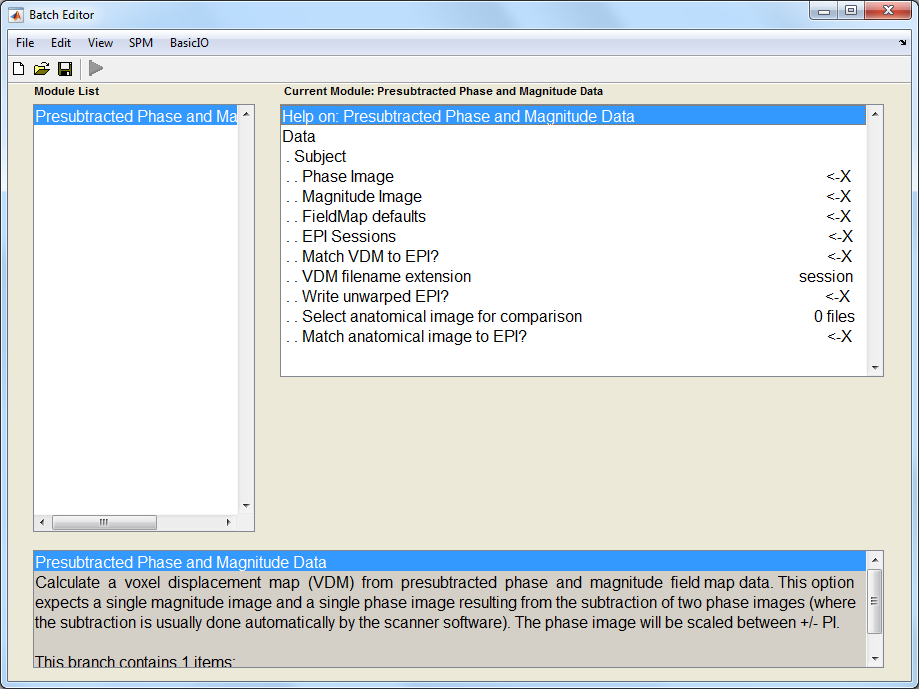
\includegraphics[width=70mm]{FieldMap/fieldmap_taskmgr}
\end{center}
\caption{FieldMap using the SPM8 User Interface.\label{FM1}}
\end{figure}

\section{Presubtracted Phase and Magnitude Data}
Calculate a voxel displacement map (VDM) from presubtracted phase and magnitude field map data (Figure \ref{FM1}). This option expects a single magnitude image and a single phase image resulting from the subtraction of two phase images (where the subtraction is usually done automatically by the scanner software). The phase image will be scaled between +/- PI.


\subsection{Data}
Subjects or sessions for which individual field map data has been acquired.


\subsubsection{Subject}
Data for this subject or field map session.


\paragraph{Phase Image}
Select a single phase image. This should be the result from the subtraction of two phase images (where the subtraction is usually done automatically by the scanner software). The phase image will be scaled between +/- PI.


\paragraph{Magnitude Image}
Select a single magnitude image. This is used for masking the phase information and coregistration with the EPI data. If two magnitude images are available, select the one acquired at the shorter echo time because it will have greater signal


\paragraph{FieldMap defaults}
FieldMap default values can be entered as a file or set of values.


\subparagraph{Defaults values}
Defaults values


\textbf{Echo times [short TE long TE]}
Enter the short and long echo times (in ms) of the data used to acquire the field map.


\textbf{Mask brain}
Select masking or no masking of the brain. If masking is selected, the magnitude image is used to generate a mask of the brain.


\textbf{Blip direction}
Enter the blip direction. This is the polarity of the phase-encode blips describing the direction in which k-space is traversed along the y-axis during EPI acquisition with respect to the coordinate system used in SPM. In this coordinate system, the phase encode direction corresponds with the y-direction and is defined as positive from the posterior to the anterior of the head.


\textbf{Total EPI readout time}
Enter the total EPI readout time (in ms). This is the time taken to acquire all of the phase encode steps required to cover k-space (ie one image slice). For example, if the EPI sequence has 64 phase encode steps, the total readout time is the time taken to acquire 64 echoes, e.g. total readout time = number of echos x echo spacing. This time does not include i) the duration of the excitation, ii) the delay between, the excitation and the start of the acquisition or iii) time for fat saturation etc.


\textbf{EPI-based field map?}
Select non-EPI or EPI based field map. The field map data may be acquired using a non-EPI sequence (typically a gradient echo sequence) or an EPI sequence. The processing will be slightly different for the two cases. If using an EPI-based field map, the resulting Voxel Displacement Map will be inverted since the field map was acquired in distorted space.


\textbf{Jacobian modulation?}
Select whether or not to use Jacobian modulation. This will adjust the intensities of voxels that have been stretched or compressed but in general is not recommended for EPI distortion correction


\textbf{uflags}
Different options for phase unwrapping and field map processing


\textsc{Unwrapping method}
Select method for phase unwrapping


\textsc{FWHM}
FWHM of Gaussian filter used to implement weighted smoothing of unwrapped maps.


\textsc{pad}
Size of padding kernel if required.


\textsc{Weighted smoothing}
Select normal or weighted smoothing.


\textbf{mflags}
Different options used for the segmentation and creation of the brain mask.


\textsc{Template image for brain masking}
Select template file for segmentation to create brain mask


\textsc{FWHM}
FWHM of Gaussian filter for smoothing brain mask.


\textsc{Number of erosions}
Number of erosions used to create brain mask.


\textsc{Number of dilations}
Number of dilations used to create brain mask.


\textsc{Threshold}
Threshold used to create brain mask from segmented data.


\textsc{Regularization}
Regularization value used in the segmentation. A larger value helps the segmentation to converge.


\subparagraph{Defaults File}
Select the 'pm\_defaults*.m' file containing the parameters for the field map data. Please make sure that the parameters defined in the defaults file are correct for your field map and EPI sequence. To create your own customised defaults file, either edit the distributed version and/or save it with the name 'pm\_defaults\_yourname.m'.


\paragraph{EPI Sessions}
If a single set of field map data will be used for multiple EPI runs/sessions, select the first EPI in each run/session. A VDM file will created for each run/session, matched to the first EPI in each run/session and saved with a unique name extension.


\subparagraph{Session}
Data for this session.


\textbf{Select EPI to Unwarp}
Select a single image to distortion correct. The corrected image will be saved with the prefix u. Note that this option is mainly for quality control of correction so that the original and distortion corrected images can be displayed for comparison. To unwarp multiple images please use either Realign \& Unwarp or Apply VDM.


\paragraph{Match VDM to EPI?}
Match VDM file to EPI image. This will coregister the field map data to the selected EPI for each run/session.


\paragraph{Name extension for run/session specific VDM file}
This will be the name extension followed by an incremented integer for run/session specific VDM files.


\paragraph{Write unwarped EPI?}
Write out distortion corrected EPI image. The image is saved with the prefix u. Note that this option is mainly for quality control of correction so that the original and distortion corrected images can be displayed for comparison. To unwarp multiple images please use either Realign \& Unwarp or Apply VDM.


\paragraph{Select anatomical image for comparison}
Select an anatomical image for comparison with the distortion corrected EPI or leave empty. Note that this option is mainly for quality control of correction.


\paragraph{Match anatomical image to EPI?}
Match the anatomical image to the distortion corrected EPI. Note that this option is mainly for quality control of correction allowing for visual inspection and comparison of the distortion corrected EPI.


\section{Real and Imaginary Data}
Calculate a voxel displacement map (VDM) from real and imaginary field map data. This option expects two real and imaginary pairs of data of two different echo times. The phase images will be scaled between +/- PI.


\subsection{Data}
Subjects or sessions for which individual field map data has been acquired.


\subsubsection{Subject}
Data for this subject or field map session.


\paragraph{Short Echo Real Image}
Select short echo real image


\paragraph{Short Echo Imaginary Image}
Select short echo imaginary image


\paragraph{Long Echo Real Image}
Select long echo real image


\paragraph{Long Echo Imaginary Image}
Select long echo imaginary image

\paragraph{Other inputs}
As for Presubtracted Phase and Magnitude Data.

\section{Phase and Magnitude Data}
Calculate a voxel displacement map (VDM) from double phase and magnitude field map data. This option expects two phase and magnitude pairs of data of two different echo times.


\subsection{Data}
Subjects or sessions for which individual field map data has been acquired.


\subsubsection{Subject}
Data for this subject or field map session.


\paragraph{Short Echo Phase Image}
Select short echo phase image


\paragraph{Short Echo Magnitude Image}
Select short echo magnitude image


\paragraph{Long Echo Phase Image}
Select long echo phase image


\paragraph{Long Echo Magnitude Image}
Select long echo magnitude image

\paragraph{Other inputs}
As for Presubtracted Phase and Magnitude Data.

\section{Precalculated FieldMap (in Hz)}
Calculate a voxel displacement map (VDM) from a precalculated field map. This option expects a processed field map (ie phase unwrapped, masked if necessary and scaled to Hz). Precalculated field maps can be generated by the FieldMap toolbox and stored as fpm\_* files.


\subsection{Data}
Subjects or sessions for which individual field map data has been acquired.


\subsubsection{Subject}
Data for this subject or field map session.


\paragraph{Precalculated field map}
Select a precalculated field map. This should be a processed field map (ie phase unwrapped, masked if necessary and scaled to Hz) , for example as generated by the FieldMap toolbox and are stored with fpm\_* prefix.


\paragraph{Select magnitude image in same space as fieldmap}
Select magnitude image which is in the same space as the field map to do matching to EPI.

\paragraph{Other inputs}
As for Presubtracted Phase and Magnitude Data.

\section{Apply VDM }
Apply VDM (voxel displacement map) to resample voxel values in selected image(s). This allows a VDM to be applied to any images which are assumed to be already realigned (e.g. including EPI fMRI time series and DTI data).

The VDM can be been created from a field map acquisition using the FieldMap toolbox and comprises voxel shift values which describe geometric distortions occuring as a result of magnetic susceptbility artefacts. Distortions along any single dimension can be corrected therefore input data may have been acquired with phase encode directions in X, Y (most typical) and Z.

The selected images are assumed to be realigned to the first in the time series (e.g. using Realign: Estimate) but do not need to be resliced. The VDM is assumed to be in alignment with the images selected for resampling (note this can be achieved via the FieldMap toolbox). The resampled images are written to the input subdirectory with the same (prefixed) filename.

e.g. The typical processing steps for fMRI time series would be 1) Realign: Estimate, 2) FieldMap to create VDM, 3) Apply VDM.

Note that this routine is a general alternative to using the VDM in combination with Realign \& Unwarp which estimates and corrects for the combined effects of static and movement-related susceptibility induced distortions. Apply VDM can be used when dynamic distortions are not (well) modelled by Realign \& Unwarp (e.g. for fMRI data acquired with R-$>$L phase-encoding direction, high field fMRI data or DTI data).


\subsection{Data}
Subjects or sessions for which VDM file is being applied to images.


\subsubsection{Session}
Data for this session.


\paragraph{Images}
Select scans for this session. These are assumed to be realigned to the first in the time series (e.g. using Realign: Estimate) but do not need to be resliced


\paragraph{Fieldmap (vdm* file)}
Select VDM (voxel displacement map) for this session (e.g. created via FieldMap toolbox). This is assumed to be in alignment with the images selected for resampling (note this can be achieved via the FieldMap toolbox).


\subsection{Reslice Options}
Apply VDM reslice options


\subsubsection{Distortion direction}
In which direction are the distortions? Any single dimension can be corrected therefore input data may have been acquired with phase encode directions in Y (most typical), X or Z


\subsubsection{Reslice which images ?}
All Images (1..n) 

  This applies the VDM and reslices all the images. 

All Images + Mean Image 

   This applies the VDM reslices all the images and creates a mean of the resliced images.


\subsubsection{Interpolation}
The method by which the images are sampled when being written in a different space. Nearest Neighbour is fastest, but not recommended for image realignment. Bilinear Interpolation is probably OK for PET, but not so suitable for fMRI because higher degree interpolation generally gives better results \cite{thevenaz00a,unser93a,unser93b}. Although higher degree methods provide better interpolation, but they are slower because they use more neighbouring voxels.


\subsubsection{Wrapping}
This indicates which directions in the volumes the values should wrap around in.  For example, in MRI scans, the images wrap around in the phase encode direction, so (e.g.) the subject's nose may poke into the back of the subject's head. These are typically:

    No wrapping - for PET or images that have already                   been spatially transformed. Also the recommended option if                   you are not really sure.

    Wrap in  Y  - for (un-resliced) MRI where phase encoding                   is in the Y direction (voxel space) etc.


\subsubsection{Masking}
Because of subject motion, different images are likely to have different patterns of zeros from where it was not possible to sample data. With masking enabled, the program searches through the whole time series looking for voxels which need to be sampled from outside the original images. Where this occurs, that voxel is set to zero for the whole set of images (unless the image format can represent NaN, in which case NaNs are used where possible).


\subsubsection{Filename Prefix}
Specify the string to be prepended to the filenames of the distortion corrected image file(s). Default prefix is 'u'.

\begin{figure}
\begin{center}
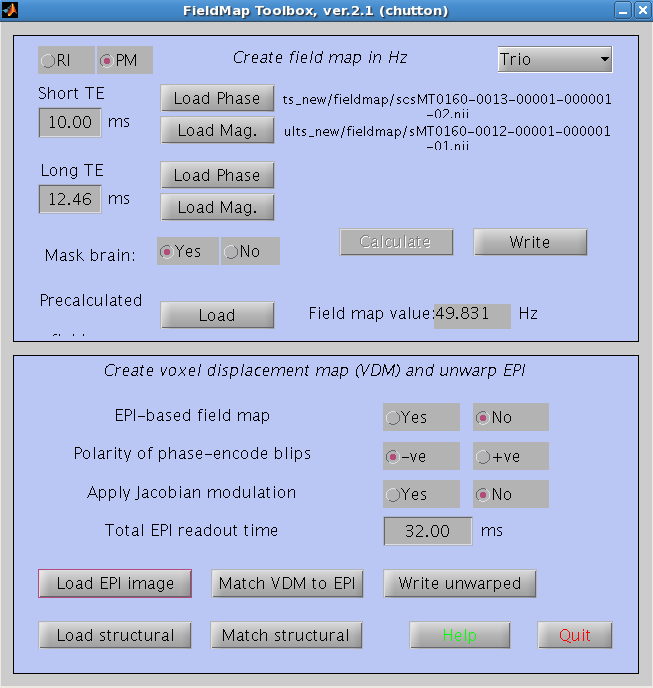
\includegraphics[width=70mm]{FieldMap/fieldmap_gui1}
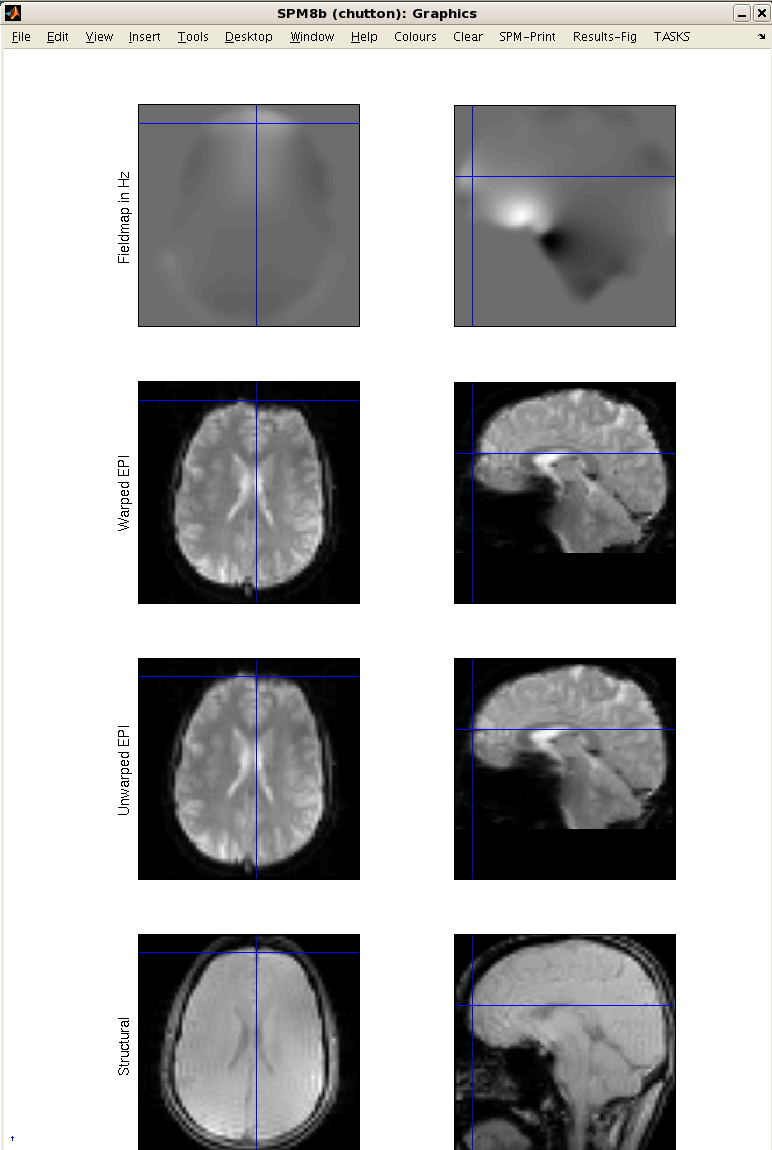
\includegraphics[width=70mm]{FieldMap/fieldmap_results1}
\end{center}
\caption{FieldMap GUI and Results. \label{FM2}}
\end{figure}

\section{Creating Field Maps Using the FieldMap GUI}
The FieldMap Toolbox GUI is shown on the left Figure \ref{FM2}. It is divided into two parts. The top part deals with creating the field map in Hz and the bottom part deals with creating the voxel displacement map (VDM) and unwarping the EPI. The toolbox can be used by working through the different inputs in the following order:

\subsection{Create field map in Hz}

\subsubsection{Load defaults file \label{loaddefs}}
Select the defaults file from which to load default parameters. If necessary, the parameters used to create the field map can be temporarily modified using the GUI. To change the default parameters, edit \texttt{pm\_defaults.m} or create a new file called \texttt{pm\_defaults\_NAME.m} (as described in Section \ref{PMDEF}).

\subsubsection{Data Input Format}
{\bf PM} The acquired field map images are in phase and magnitude format. There may be a single pair of phase and magnitude images (i.e. 2 images) in which case the phase image has been created by the vendor sequence from two echo times acquisitions. Alternatively there may be two pairs of phase and magnitude images, one for each echo time(ie 4 images). The units for the phase images MUST BE RADIANS BETWEEN +pi and -pi. The user will be asked if this is required when the images are selected.

{\bf RI} The acquired field map images are in real and imaginary format. Two pairs of real and imaginary image volumes, one for a shorter and one for a longer echo time (ie 4 images)\footnote{
NB If using SPM2, the data input format can only be changed by editing the spm\_defaults.m file. This is described in Section \ref{PMDEF}.}.

\subsubsection{File Selection}
Select NIfTI format images. Generally, the acquired scanner files will be in dicom format which can be correctly converted using the DICOM converter in the corresponding version of SPM. DICOM and other image formats can also be converted to using MRIcro\footnote{MRIcro is freely available from \url{http://www.cla.sc.edu/psyc/faculty/rorden/mricro.html}.}.

If the data input format is PM, load Phase and Magnitude images:
\begin{enumerate}
\item{Single phase image OR phase of short echo-time image.}
\item{Single magnitude image OR magnitude of short echo-time image.}
\item{LEAVE EMPTY if input consists of a single phase and magnitude pair OR phase of long echo-time image.}
\item{LEAVE EMPTY if input consists of a single phase and magnitude pair OR magnitude of long echo-time image.}
\end{enumerate}
OR 
If the data input format is RI, load Real and Magnitude images:
\begin{enumerate}
\item{Real part of short echo-time image.}
\item{Imaginary part of short echo-time image.}
\item{Real part of long echo-time image.}
\item{Imaginary part of long echo-time image.}
\end{enumerate}

\subsubsection{Short TE/Long TE (ms)}
Specify the short and long echo times in ms associated with the field map acquisition. Both of these values are required even if a single phase and magnitude image is used as input.

\subsubsection{Mask brain}
Specify yes to generate a brain mask using the magnitude data which will be used to exclude regions of the field map outside of the brain.

\subsubsection{Calculate}
Calculate an unwrapped field map in Hz which is stored in memory. This represents the map of phase changes associated with the measured field map data. The processing is described in more detail in Section \ref{FMAppendix} and involves some or all of the following steps (as specified in spm\_defaults.m): 
\begin{enumerate}
\item{Calculation of a Hz fieldmap from input data}
\item{Segmentation to exclude regions outside of the brain}
\item{Phase unwrapping}
\item{Smoothing and dilation of the processed fieldmap}
\end{enumerate}

The processed field map (in Hz) is displayed in the graphics window (top row, right Figure \ref{FM1}) and the field at different points can be explored. The field map in Hz is converted to a VDM (voxel displacement map) using the parameters shown in the FieldMap GUI and saved with the filename vdm5\_NAME-OF-FIRST-INPUT-IMAGE.img in the same directory as the acquired field map images. The VDM file is overwritten whenever the field map is recalculated or when any parameters are changed. The resulting VDM file can be used for unwarping the EPI using Realign \& Unwarp in SPM8 (see Section \ref{VDMuse}).

\subsubsection{Write}
Write out the processed field map (in Hz) as a Nifti format image. The image will be saved with the filename fpm\_NAME-OF-FIRST-INPUT-IMAGE.img in the same directory as the acquired field map images.

\subsubsection{Load Pre-calculated}
Load a precalculated unwrapped field map (\texttt{fpm\_\*.img}). This should be a single image volume with units of Hz in NIfTI format. The precalculated field map may have been created previously using the FieldMap toolbox or by other means. Once loaded, the field map is displayed in the graphics window (top row, right, Figure \ref{FM1}) and the field at different points can be explored.

\subsubsection{Field map value (Hz)}
Interrogate the value of the field map in Hz at the location specified by the mouse pointer in the graphics window.

\subsection{Create voxel displacement map (VDM) and unwarp EPI}

When any of the parameters below are changed, a new VDM is created and written out as vdm5\_NAME-OF-FIRST-INPUT-IMAGE.img. The vdm5\_NAME-OF-FIRST-INPUT-IMAGE.mat file is not updated unless 'Match VDM to EPI' is selected as described in Section \ref{VDMmatch}.

\subsubsection{EPI-based field map - Yes/No}
Select Yes if the field map is based on EPI data or No otherwise. Most scanner vendor field map sequences are non-EPI.

\subsubsection{Polarity of phase-encode blips - +ve/-ve}
Select +ve or -ve blip direction.When images are acquired K-space can be traversed using positive or negative phase-encode blips. This direction will influence the geometric distortions in terms of whether the affected regions of the image are stretched or compressed. 

The convention used to describe the direction of the k-space traversal is based on the coordinate system used by SPM. In this coordinate system, the phase encode direction corresponds with the y-direction and is defined as positive from the posterior to the anterior of the head. The x-direction is defined as positive from left to right and the z-direction is defined as positive from foot to head. The polarity of the phase-encode blips describes in which direction k-space is traversed along the y-axis with respect to the coordinate system described here. 

\subsubsection{Apply Jacobian modulation - Yes/No}
Select Yes to do Jacobian Modulation to adjust the intensities of voxels that have been stretched or compressed. In general this is not recommended for unwarping EPI data at this stage.

\subsubsection{Total EPI readout time (ms)}
Enter the total time in ms for the readout of the EPI echo train which is typically 10s of ms. This is the time taken to acquire all of the phase encode steps required to cover k-space (ie one image slice). For example, if the EPI sequence has 64 phase encode steps, the total readout time is the time taken to acquire 64 echoes: 
        total readout time = number of echoes $\times$ echo spacing.
This time does not include i) the duration of the excitation, ii) the delay between the excitation and the start of the acquisition or iii) time for fat saturation.

\subsubsection{Load EPI image}
Select a sample EPI image in NIfTI format. This image is automatically unwarped using the VDM calculated with the current parameters. The warped and the unwarped image are displayed in the graphics window underneath the field map (middle rows, right, Figure \ref{FM1}).

\subsubsection{Match VDM to EPI \label{VDMmatch}}
Select this option to match the field map magnitude data to the EPI image before it is used to unwarp the EPI. In general, the field map data should be acquired so that it is as closely registered with the EPI data as possible but matching can be selected if required. If a precalculated field map was loaded then the user is prompted to select a magnitude image in the same space as the field map. If real and imaginary images were selected, the toolbox automatically creates a magnitude image from these images and saves it with the name mag\_NAME-OF-FIRST-INPUT-IMAGE.img. 

\subsubsection{Write unwarped}
Write unwarped EPI image with the filename \texttt{uNAME\_OF\_EPI.img}.

\subsubsection{Load structural}
Load a structural image for comparison with unwarped EPI. This is displayed in the graphics window below the other images (bottom row, right fig 1).

\subsubsection{MatchStructural}
Coregister the structural image to the unwarped EPI and write the resulting transformation matrix to the header of the selected structural image.

\subsubsection{Help}
Call \texttt{spm\_help} to display \texttt{FieldMap.man}.

\subsubsection{Quit}
Quit the toolbox and closes all windows associated with it.


\section{Using the FieldMap in Batch scripts}
\texttt{FieldMap\_preprocess.m} which calls \texttt{FieldMap\_create.m} gives an example of how to run the FieldMap toolbox without using the GUI. To run the script, make sure your \matlab\ path includes the directory where the FieldMap toolbox is installed. This can be done using the Set Path option under File in the \matlab\ windows manager or using the command: 
\begin{verbatim}
addpath /whatever/spm/toolbox/FieldMap
\end{verbatim}

To run the FieldMap batch script, in \matlab\ enter the following command: 
\begin{verbatim}
VDM = FieldMap_preprocess(fm_dir,epi_dir, [te1, te2, epifm, tert, kdir, mask, match] );
\end{verbatim}
where

\emph{fm\_dir} - name of directory containing fieldmap images.(e.g. fm\_dir = '/path/study1/subj1/fieldmap') 

\emph{epi\_dir} - name of directory containing epi images. (e.g. epi\_dir = '/path/study1/subj1/images')

\emph{te1} - short echo time (in ms)

\emph{te2} - long echo time (in ms)

\emph{epifm} - epi-based fieldmap - yes or no (1/0)

\emph{tert} - total echo readout time (in ms)

\emph{kdir} - blip direction (1/-1)

\emph{mask} do brain segmentation to mask field map (1/0)

\emph{match} match vdm file to first EPI in run (1/0).

NB: FieldMap will match the field map to the first epi image in the time series (after removing the dummy scans). Therefore, epi\_dir must be the directory that contains the epi run that all other images will be realigned to.

The script will create an fpm* file, a vdm5\_* file and an unwarped version of the EPI saved with the prescript ``u''.

\section{Using the VDM file with Unwarp \label{VDMuse}}
In SPM, select the Realign \& Unwarp option. For the input data called Phase map (vdm* file), select the vdm5\_\* or vdm5\_\* file for the subject and/or session. If you acquired more than one session (or run) of EPI images, you need to select a different vdm5\_* file for each one. For more information about Unwarp see \url{http://www.fil.ion.ucl.ac.uk/spm/toolbox/unwarp}.

\section{Appendices\label{FMAppendix}}

\subsection{Processing Hz field maps}
Processing field maps involves a series of steps for which certain parameters in the spm\_defaults file must be set.
\begin{enumerate}
\item{If the acquired field map data comprises two complex images, the phase difference between them is calculated. 
}
\item{The phase map is unwrapped using the method specified by spm\_def.UNWRAPPING\_METHOD = 'Mark3D' or 'Mark2D' or 'Huttonish'. For a description of these different methods see spm\_unwrap.m or FieldMap\_principles.man. The default option is 'Mark3D'.
}
\item{A mask is created so that unwrapping only occurs in regions where there is signal. If necessary, this mask can be expanded so that any voxel that hasn't been unwrapped and is less than spm\_def.PAD/2 voxels away from an unwrapped one will be replaced by an average of the surrounding unwrapped voxels. This can be done by setting the parameter spm\_def.PAD to a value greater than 0. The default value is 0 but a value > 0 (eg 10) may be necessary if normal smoothing is chosen instead of weighted smoothing (as explained in the next step). 
}
\item{If required a mask can be generated to exclude regions of the fieldmap outside of the brain (in addition to the unwrapping mask described above). This step uses SPM segmentation for which the parameters in spm\_def.MFLAGS can be set. For example, if the segmentation fails, (maybe because the fieldmap magnitude image doesn't have enough contrast), spm\_def.MFLAGS.REG can be increased to say 0.05). The other parameters control morphological operations to generate a smooth brain mask and have been set empirically.
}
\item{The unwrapped phase map is scaled by 1/(2*PI*difference in echo time) to convert it to Hz.
}
\item{A weighted gaussian smoothing (weighted by the inverse of the noise) is performed on the unwrapped phase-map if the parameter spm\_def.WS = 1. If spm\_def.WS = 0, a normal smoothing is done. The weighted smoothing is particularly slow on large data sets ie high resolution. If field maps are acquired at high resolution then it is recommended to use spm\_def.WS = 0 and do some padding of the intensity mask eg spm\_def.PAD = 10. The size of the Gaussian filter used to implement either weighted or normal smoothing of the unwrapped maps is usually set to spm\_def.FWHM = 10.
}
\end{enumerate}

\subsection{Converting Hz field map to VDM}
\begin{enumerate}
\item{The field map in Hz is multiplied by the total EPI readout time (in ms, ) of the EPI image to be unwarped, resulting in a VDM. The readout time is specified by spm\_def.TOTAL\_EPI\_READOUT\_TIME (eg typically 10s of ms).The total EPI readout time is the time taken to acquire all of the phase encode steps required to cover k-space (ie one image slice). For example, if the EPI sequence has 64 phase encode steps, the total readout time is the time taken to acquire 64 echoes, e.g. total readout time = number of echoes $\times$ echo spacing. This time does not include i) the duration of of the excitation, ii) the delay between the excitation and the start of the acquisition or iii) time for fat saturation etc.
}
\item{The VDM is multiplied by +/-1 to indicate whether the K-space traversal for the data acquisition has a +ve or -ve blip direction. This will ensure that the unwarping is performed in the correct direction and is specified by spm\_def.K\_SPACE\_TRAVERSAL\_BLIP\_DIR = +/- 1.
}
\item{The toolbox must know if the field map is based on an EPI or non-EPI acquisition. If using an EPI-based field map, the VDM must be inverted since the field map was acquired in warped space. This is specified by spm\_def.EPI\_BASED\_FIELDMAPS = 1 or 0.
}
\item{Jacobian Modulation can be applied to the unwarped EPI image. This modulates the intensity of the unwarped image so that in regions where voxels were compressed, the intensity is decresed and where voxels were stretched, the intensities are increased slightly. The modulation involves multiplying the unwarped EPI by 1 + the 1-d derivative of the VDM in the phase direction. An intensity adjustment of this nature may improve the coregistration results between an unwarped EPI and an undistorted image. This is specified by spm\_def.DO\_JACOBIAN\_MODULATION = 0 or 1.   
}
\item{When any of the above conversion parameters are changed or a new EPI is selected, a new VDM is created and saved with the filename vdm5\_NAME-OF-FIRST-INPUT-IMAGE.img. Any previous copy of the .img file is overwritten, but the corresponding .mat file is retained. It is done this way because the VDM may have already been coregiseterd to the EPI (as described below). Then, for an EPI-based VDM, the match between the VDM and the EPI will still be valid even if any of the above parameters have been changed. If the VDM is non-EPI-based and any of the above parameters are changed, the match between the VDM and the EPI may no longer be valid. In this case a warning is given to the user that it may be necessary to perform the coregistration again.
}
\end{enumerate}
 
\subsection{Matching field map data to EPI data}
\begin{enumerate}
\item{If required, the fieldmap can be matched to the EPI. This is done slightly differently depending on whether the field map is based on EPI or non-EPI data. If using an EPI field map, the magnitude image is coregistered to the EPI. The resulting transformation matrix is used to sample the VDM file in the space of the EPI before unwarping. 
}
\item{If using a non-EPI field map, the VDM is used to forward warp the magnitude image which is then coregistered to the EPI. The forward warped image is saved with the filename wfmag\_NAME-OF-FIRST-INPUT-IMAGE.img. 
}
\end{enumerate}



%\include{unused}
%\include{cat}

%%%%%% DATASETS %%%%%%

\part{Data sets and examples}

\chapter{Auditory fMRI data \label{Chap:data:auditory}}
 
This data set comprises whole brain BOLD/EPI images acquired on a modified 2T Siemens MAGNETOM Vision system. Each acquisition consisted of 64 contiguous slices (64$\times$64$\times$64 3$\times$3mm$\times$3 mm$^3$ voxels). Acquisition took 6.05s, with the scan to scan repeat time (TR) set arbitrarily to 7s.

96 acquisitions were made (TR=7s) from a single subject, in blocks of 6, giving 16 42s blocks. The condition for successive blocks alternated between rest and auditory stimulation, starting with rest. Auditory stimulation was bi-syllabic words presented binaurally at a rate of 60 per minute. The functional data starts at acquisition 4, image \texttt{fM00223\_004}. Due to T1 effects it is advisable to discard the first few scans (there were no ``dummy'' lead-in scans). A structural image was also acquired: \texttt{sM00223\_002}. These images are stored in Analyze format and are available from the SPM site \footnote{Auditory fMRI data: \url{http://www.fil.ion.ucl.ac.uk/spm/data/}}. This data set was the first ever collected and analysed in the Functional Imaging Laboratory (FIL) and is known locally as the mother of all experiments (MoAE).

To analyse the data, first create a new directory \texttt{DIR},  eg. \texttt{c:$\backslash$data$\backslash$auditory}, in which to place the results of your analysis. Then create 3 subdirectories (i) \texttt{jobs}, (ii) \texttt{classical} and (iii) \texttt{bayesian}. As the analysis proceeds these directories will be filled with job-specification files, design matrices and models estimated using classical or Bayesian methods.

Start up \matlab\, enter your jobs directory and type \texttt{spm fmri} at the \matlab\ prompt. SPM will then open in fMRI mode with three windows (1) the top-left or ``Menu'' window, (2) the bottom-left or ``Interactive'' window and (3) the right-hand or ``Graphic'' window. Analysis then takes place in three major stages (i) spatial pre-processing, (ii) model specification, review and estimation and (iii) inference. These stages organise the buttons in SPM's base window.

\begin{figure}
\begin{center}
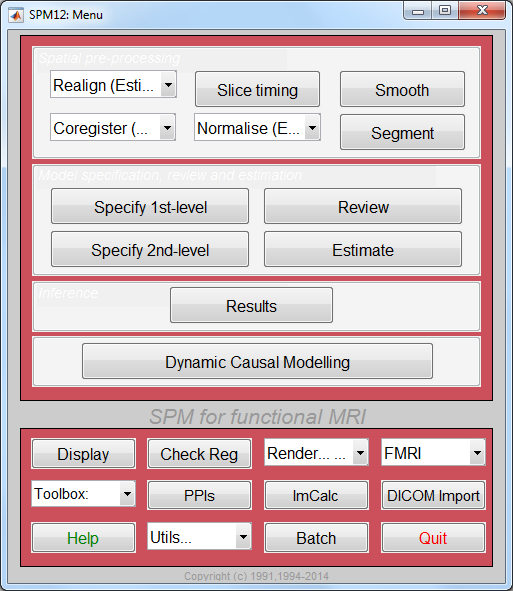
\includegraphics[width=100mm]{auditory/command}
\caption{\em The SPM base window comprises three sections i) spatial pre-processing, (ii) model specification, review and estimation and (iii) inference. \label{aud_command}}
\end{center}
\end{figure}

\section{Spatial pre-processing}

\subsection{Realignment}

Under the spatial pre-processing section of the SPM base window select textsc{Realign (Est \& Res)} from the \textsc{Realign} pulldown menu. This will call up a realignment job specification in the batch editor. Then
\begin{itemize}
\item Highlight data, select ``New Session'', then highlight the newly created ``Session'' option.
\item Select ''Specify Files'' and use the SPM file selector to choose all of your functional images eg. ``\texttt{fM000*.img}''. There should be 96 files.
\item Save the job file as eg. \texttt{DIR$\backslash$jobs$\backslash$realign.mat}.
\item Press the \texttt{RUN} button in the batch editor (green arrow).
\end{itemize}

This will run the realign job which will write realigned images into the directory where the functional images are. These new images will be prefixed with the letter ``\texttt{r}''. SPM will then plot the estimated time series of translations and rotations shown in Figure~\ref{aud_realign}. These data are also saved to a file eg. \texttt{rp\_fM00223\_004.txt}, so that these variables can be used as regressors when fitting GLMs. This allows movements effects to be discounted when looking for brain activations.

SPM will also create a mean image eg. \texttt{meanfM00223\_004.img} which will be used in the next step of spatial processing - coregistration.

\begin{figure}
\begin{center}
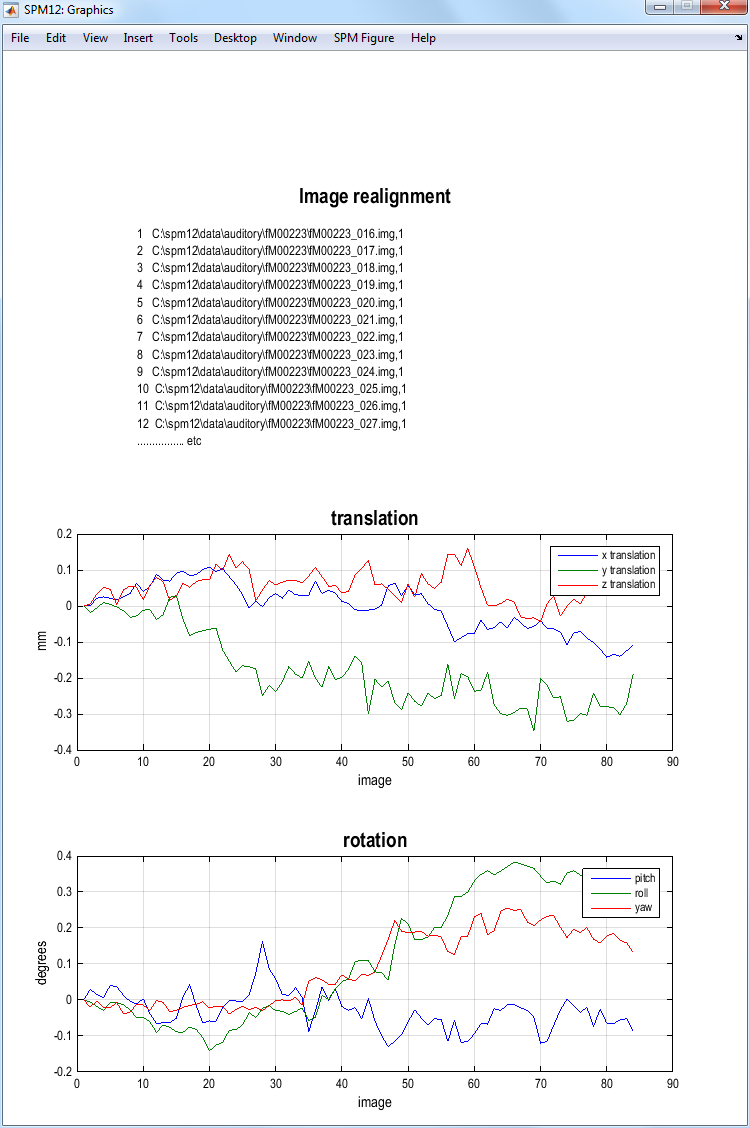
\includegraphics[width=100mm]{auditory/realign}
\caption{\em Realignment of Auditory data.\label{aud_realign}}
\end{center}
\end{figure}

\subsection{Coregistration}

Select \textsc{Coregister (Estimate)} from the \textsc{Coregister} pulldown. This will call up the specification of a coregistration job in the batch editor. 

\begin{itemize}
\item Highlight ``Reference Image'' and then select the mean fMRI scan from realignment eg. \texttt{meanfM00223\_004.img}.
\item Highlight ``Source Image'' and then select the structural image eg. \texttt{sM00223\_002.img}.
\item Press the Save button and save the job as \texttt{coreg.job}.
\item Then press the \texttt{RUN} button.
\end{itemize}

SPM will then implement a coregistration between the structural and functional data that maximises the mutual information. The image in figure~\ref{aud_coreg} should then appear in the graphics window. SPM will have changed the header of the source file which in this case is the structural image \texttt{sM00223\_002.hdr}.
\begin{figure}
\begin{center}
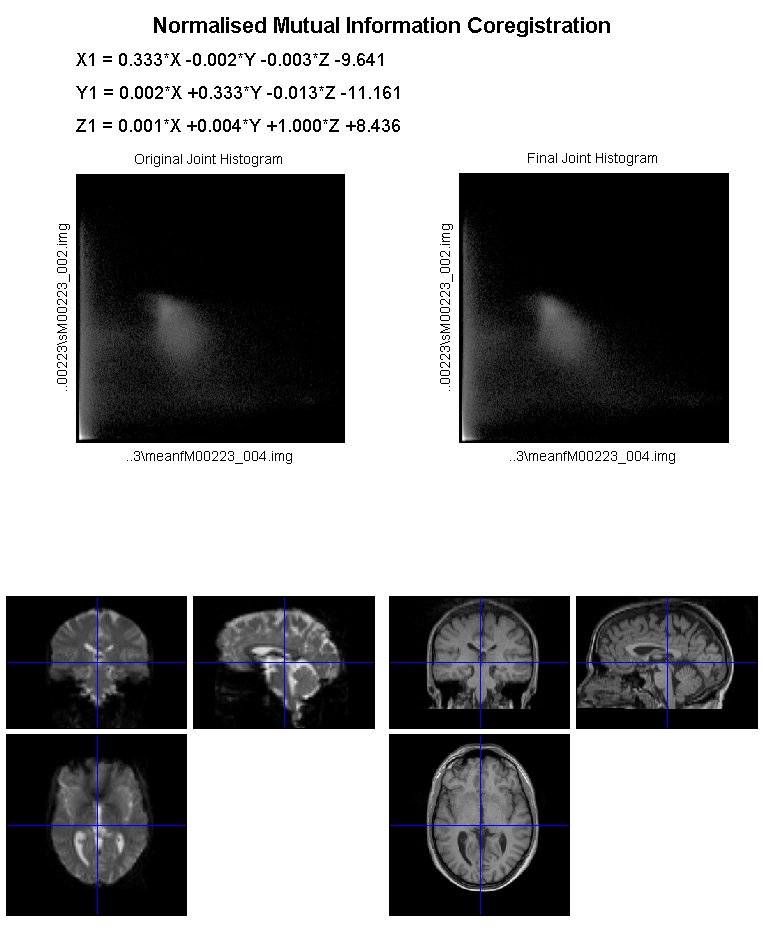
\includegraphics[width=100mm]{auditory/coreg}
\caption{\em Mutual Information Coregistration of Auditory data.\label{aud_coreg}}
\end{center}
\end{figure}

The \textsc{Check Reg} facility is useful here, to check the results of coregistration. Press the \textsc{Check Reg} button in the lower section of the base window and then the select the ``Reference'' and ``Source'' Images specified above ie \texttt{meanfM00223\_004.img} and \texttt{sM00223\_002.img}. SPM will then produce an image like that shown in Figure~\ref{aud_checkreg} in the Graphics window. You can then use your mouse to navigate these images to confirm that there is an anatomical correspondence.

\begin{figure}
\begin{center}
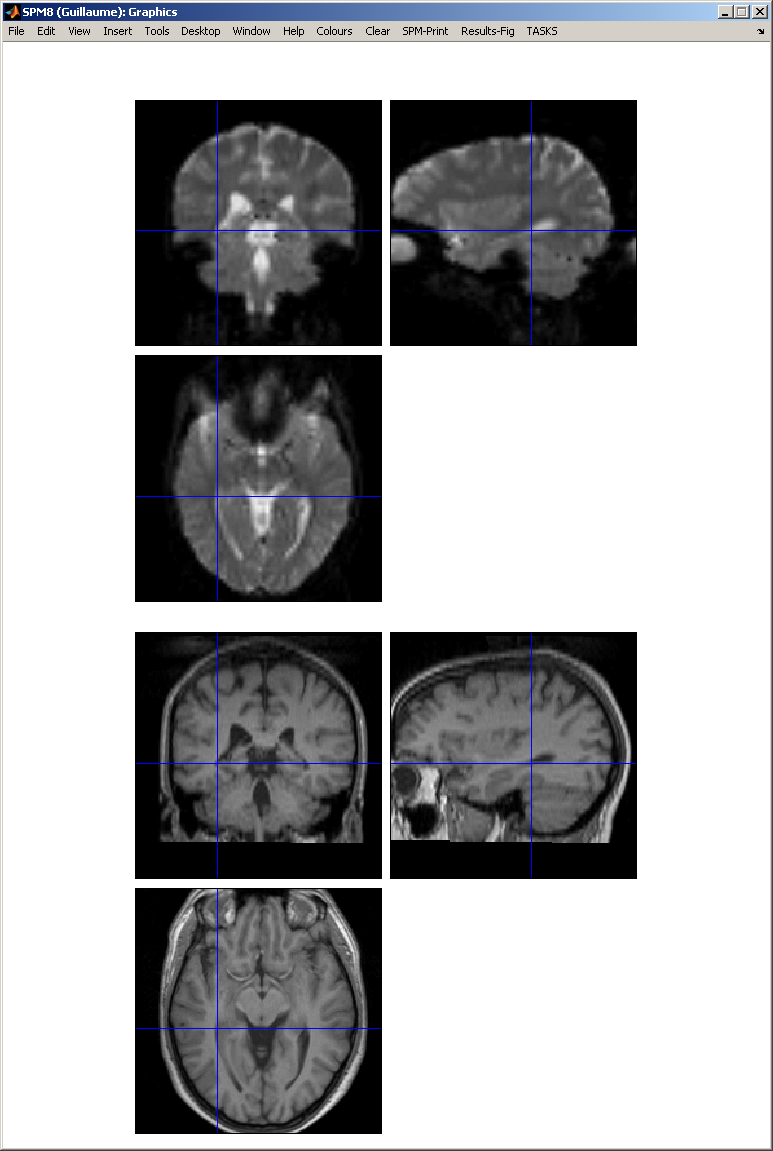
\includegraphics[width=100mm]{auditory/checkreg}
\caption{\em Checking registration of functional and ``registered'' structural data. \label{aud_checkreg}}
\end{center}
\end{figure}

\subsection{Segmentation}

Press the \textsc{Segment} button. This will call up the specification of a segmentation job in the batch editor. Highlight the Data field and then select the subjects registered anatomical image eg. \texttt{sM00223\_002.img}. Save the job file as \texttt{segment.mat} and then press \texttt{RUN}. SPM will segment the structural image using the default tissue probability maps as priors. 

Faster, though perhaps less optimal results can be obtained by eg. reducing the number of Gaussians per class from [2 2 2 4] to eg. [1 1 1 4], increasing the sampling distance from eg. 3 to 4mm. These options can be edited under the ``Custom'' sub-menu and saved before the job is run. The results obtained in figure~\ref{aud_gray} were obtained using the default values.

SPM will create, by default, gray and white matter images and bias-field corrected structural image. These can be viewed using the CheckReg facility as described in the previous section. Figure~\ref{aud_gray} shows the gray matter image, \texttt{c1sM0023\_002.img} along with the original structural. Figure~\ref{aud_bias} shows the structural and bias-corrected image, \texttt{msM0023\_002.img}.

\begin{figure}
\begin{center}
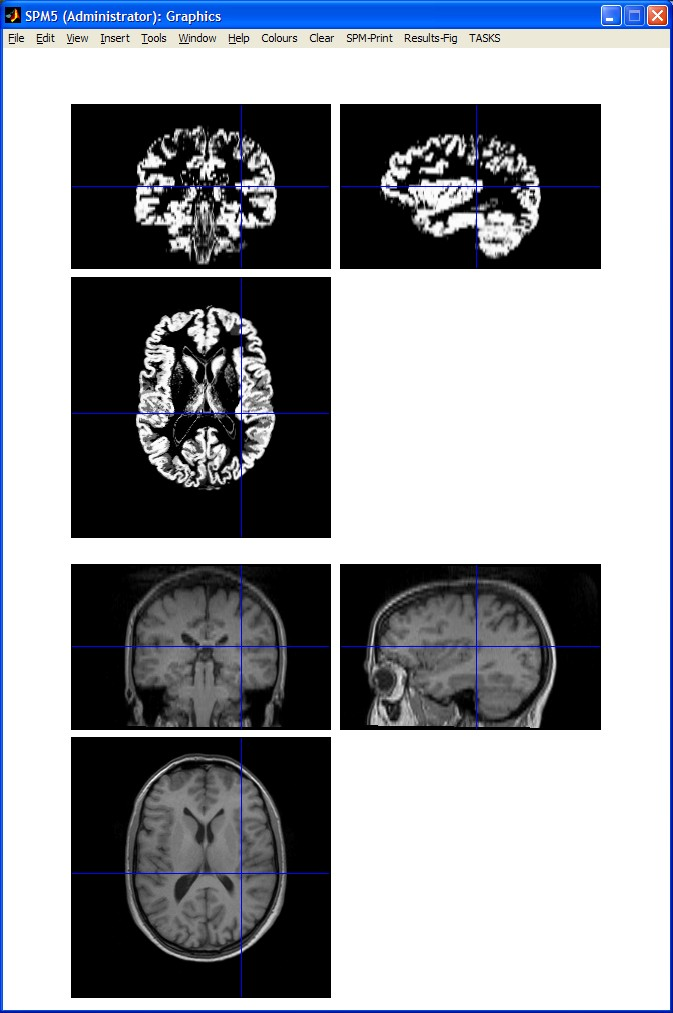
\includegraphics[width=100mm]{auditory/gray}
\caption{\em Gray matter image and ``registered'' structural image.\label{aud_gray}}
\end{center}
\end{figure}

\begin{figure}
\begin{center}
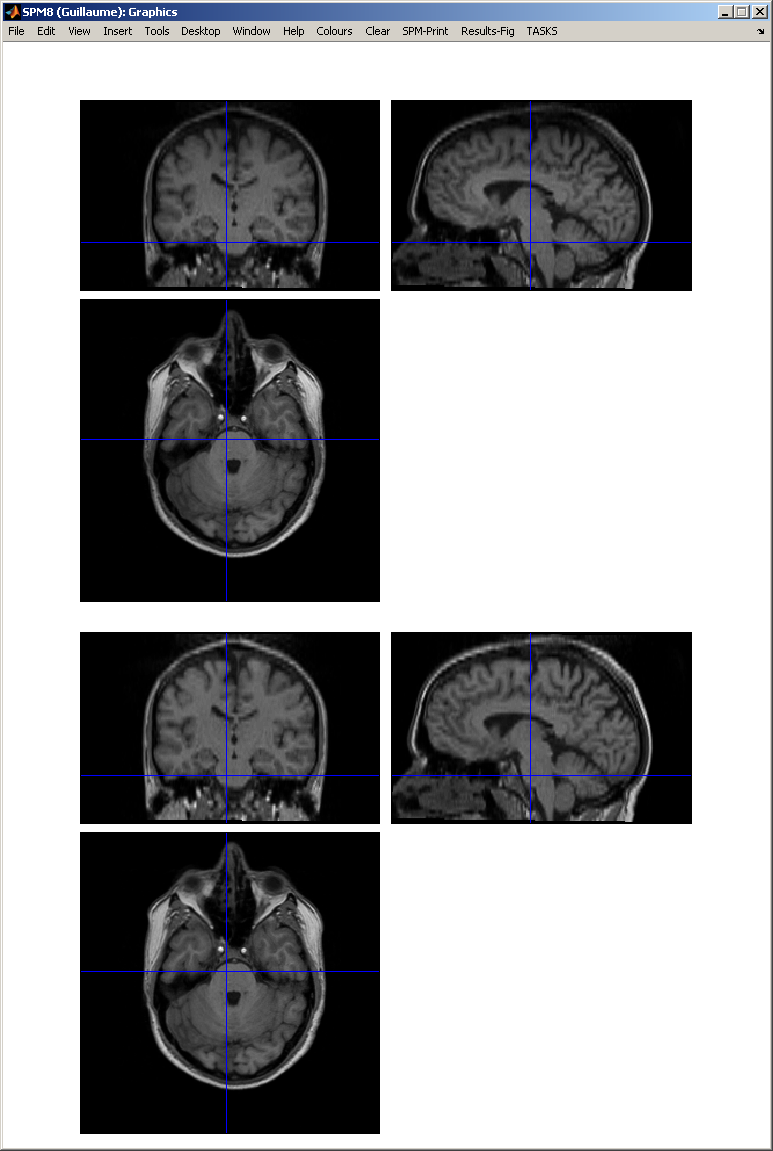
\includegraphics[width=100mm]{auditory/bias}
\caption{\em Structural image (top) and bias-corrected structural image (bottom). Notice that the original structural is darker at the top than at the bottom. This non-uniformity has been removed in the bias-corrected image.\label{aud_bias}}
\end{center}
\end{figure}

SPM will also write a spatial normalisation eg. \texttt{sM00223\_0020\_seg\_sn.mat} and inverse spatial normalisation parameters \texttt{sM00223\_0020\_seg\_inv\_sn.mat} to files in the original structural directory. These can be used to normalise the functional data. 

\subsection{Normalise}

Select \textsc{Normalise (Write)} from the \textsc{Normalise} pulldown menu. This will call up the specification of a normalise job in the batch editor. 

\begin{itemize}
\item Highlight ``Data'', select New ``Subject'',
\item Highlight ``Parameter File'' and select the \texttt{sM00223\_0020\_seg\_sn.mat} file that you created in the previous section,
\item Highlight images to write and select all of the realigned functional images \texttt{rfM000*.img}. Note: This can be done efficiently by changing the filter in the SPM file selector to \texttt{\^r.*}. SPM will then only list those files beginning with the letter \texttt{r} ie. those that have been realigned. You can then right click over the listed files, choose ``Select all'' and press ``Done''.
\item Open ``Writing Options'', and change ``Voxel sizes'' from [2 2 2] to [3 3 3].\footnote{This step is not strictly necessary. It will write images out at a resolution closer to that at which they were acquired. This will speed up subsequent analysis and is necessary, for example, to make Bayesian fMRI analysis computationally efficient.}
\item Press ``Save'', save the job as \texttt{normalise.mat} and then press the \texttt{RUN} button.
\end{itemize}

SPM will then write spatially normalised files to the functional data directory. These files have the prefix \texttt{w}.

If you wish to superimpose a subject's functional activations on their own anatomy\footnote{Beginners may wish to skip this step, and instead just superimpose functional activations on an ``average structural image''.} you will also need to apply the spatial normalisation parameters to their (bias-corrected) anatomical image. To do this

\begin{itemize}
\item Select \textsc{Normalise (Write)}, highlight ``Data'', select ``New Subject''.
\item Highlight ``Parameter File'', select the  \texttt{sM00223\_0020\_seg\_sn.mat} file that you created in the previous section, press ``Done''.
\item Highlight ``Images to Write'', select the bias-corrected structural eg. \texttt{msM00223\_002.img}, press ``Done''.
\item Open ``Writing Options'', select voxel sizes and change the default [2 2 2] to [1 1 3] which corresponds to the original resolution of the images.
\item Save the job as \texttt{norm\_struct.mat} and press the \texttt{Run} button.
\end{itemize}

\subsection{Smoothing}

Press the \textsc{Smooth} button\footnote{The smoothing step is unnecessary if you are only interested in Bayesian analysis of your functional data.}. This will call up the specification of a smooth job in the batch editor.

\begin{itemize}
\item Select ``Images to Smooth'' and then select the spatially normalised files created in the last section eg. \texttt{\^wrf.*}.
\item Highlight ``FWHM'' and change [8 8 8] to [6 6 6]. This will smooth the data by 6mm in each direction.
\item Save the job as \texttt{smooth.mat} and press the \texttt{Run} button.
\end{itemize}

An example of functional image and its smoothed version is displayed on Figure~\ref{aud_smooth}.

\begin{figure}
\begin{center}
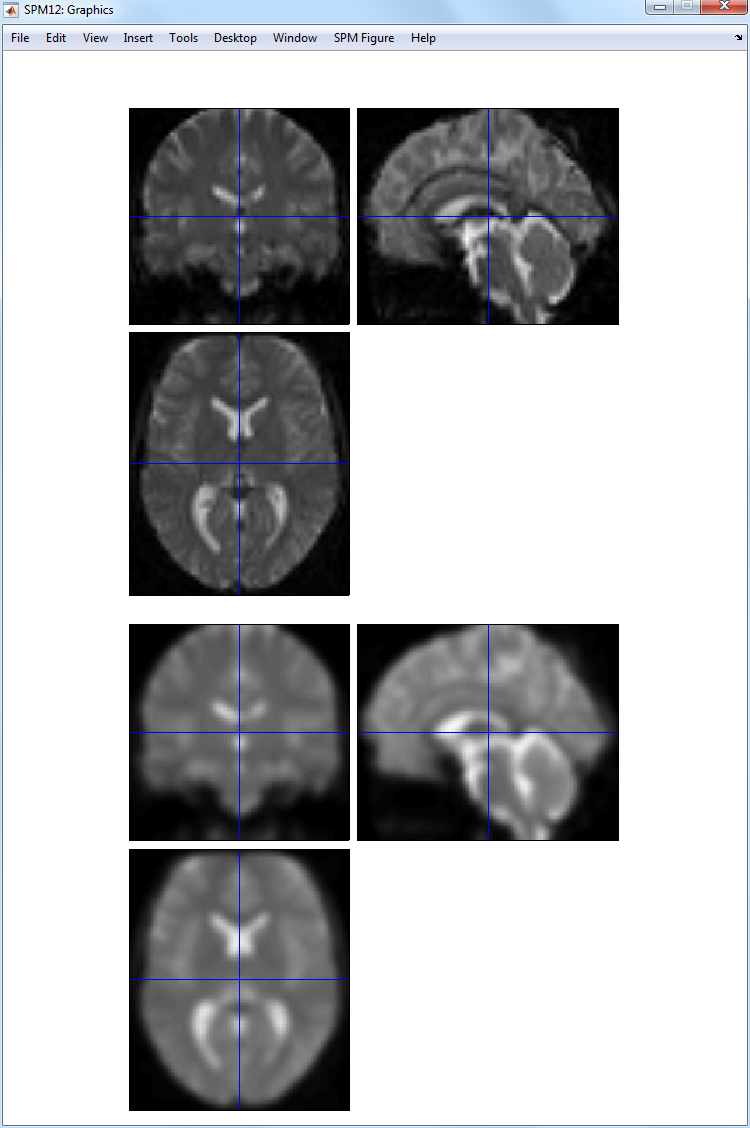
\includegraphics[width=100mm]{auditory/smooth}
\caption{\em Functional image (top) and 6mm-smoothed functional image (bottom). These images were obtained using SPM's ``CheckReg'' facility. \label{aud_smooth}}
\end{center}
\end{figure}

\section{Model specification, review and estimation}

To avoid T1 effects in the initial scans of an fMRI time series we recommend discarding the first few scans. To make this example simple, we'll discard the first complete cycle (12 scans, 04-15), leaving 84 scans, image files 16-99. This is best done by moving these files to a different directory.

Press the ``Specify 1st-level'' button. This will call up the specification of an fMRI specification job in the batch editor. Then

\begin{itemize}
\item Open the ``Timing parameters'' option.
\item Highlight ``Units for design'' and select ``Scans''.
\item Highlight ``Interscan interval'' and enter 7.
\item Highlight ``Data and Design'' and select ``New Subject/Session''. Then open the newly created ``Subject/Session'' option.
\item Highlight ``Scans'' and use SPM's file selector to choose the 84 smoothed, normalised functional images ie  \texttt{swrfM00223\_016.img} to \texttt{swrfM00223\_099.img}. These can be selected easily using the \texttt{\^s.*'} filter, and select all (provided you have moved the scans 4 to 15 into a different directory). Then press ``Done''.
\item Highlight ``Condition'' and select ``New condition''.
\item Open the newly created ``Condition'' option. Highlight ``Name'' and enter ``active''. Highlight ``Onsets'' and enter ``6:12:84''. Highlight ``Durations'' and enter ``6''.
\item Highlight ``Directory'' and select the \texttt{DIR/classical} directory you created earlier.
\item Save the job as \texttt{specify.mat} and press the \texttt{Run} button.
\end{itemize}

SPM will then write an \texttt{SPM.mat} file to the \texttt{DIR/classical} directory. It will also plot the design matrix, as shown in Figure~\ref{aud_design}. 

\begin{figure}
\begin{center}
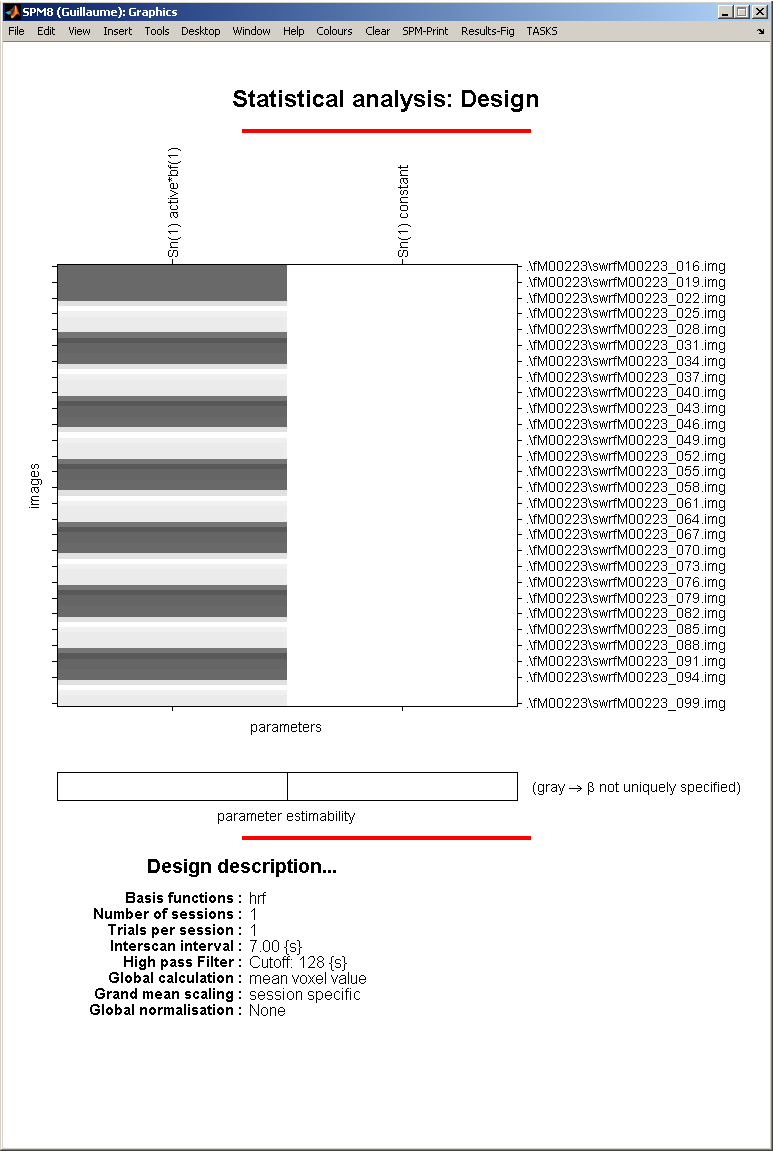
\includegraphics[width=80mm]{auditory/design}
\caption{\emph{\texttt{Design matrix}: The filenames on the right-hand side of the design matrix indicate the scan associated with each row.\label{aud_design}}}
\end{center}
\end{figure}

At this stage it is advisable to check your model specification using SPM's review facility which is accessed via the ``Review'' button. This brings up a ``design'' tab on the interactive window clicking on which produces a pulldown menu. If you select the first item ``Design Matrix'' SPM will produce the image shown in Figure~\ref{aud_design}. If you select ``Explore'' then ``Session 1'' then ``active'', SPM will produce the plots shown in Figure~\ref{aud_explore}.

\begin{figure}
\begin{center}
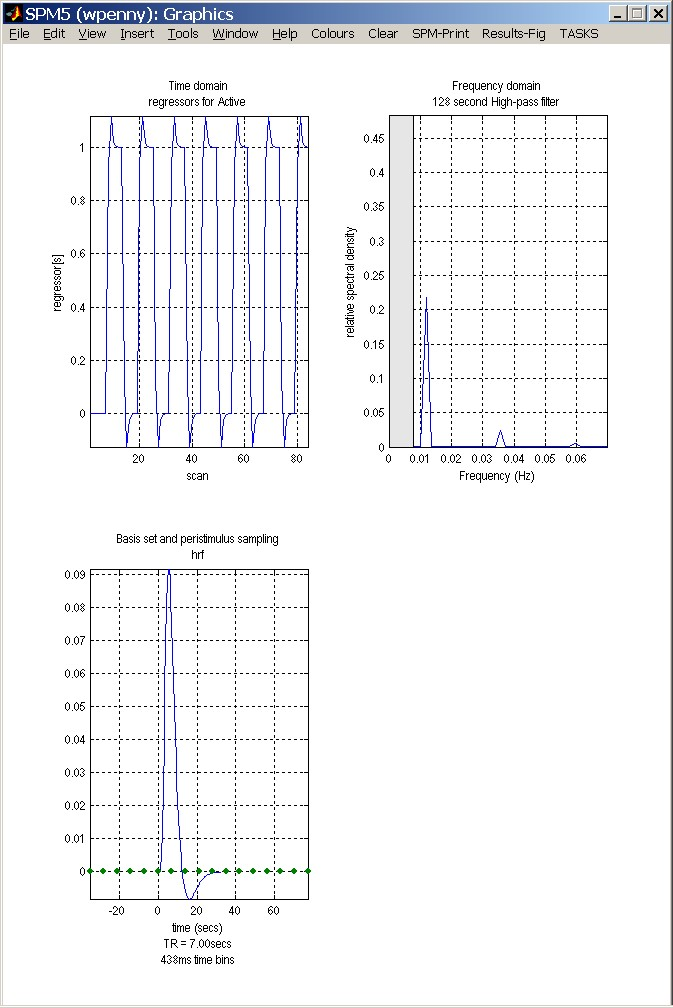
\includegraphics[width=80mm]{auditory/explore}
\caption{\emph{\texttt{Exploring the design matrix in Figure~\ref{aud_design}}: This shows the time series of the ``active'' regressor (top left), a frequency domain plot of the active regressor (top right) and the basis function used to convert assumed neuronal activity into hemodynamic activity. In this model we used the default option - the canonical basis function. The frequency domain plot shows that the frequency content of the ``active'' regressor is above the set frequencies that are removed by the High Pass Filter (HPF) (these are shown in gray - in this model we accepted the default HPF cut-off of 128s or 0.008Hz). \label{aud_explore}}}
\end{center}
\end{figure}

If you select the second item on the ``Design'' tab, ``Design Orthogonality'', SPM will produce the plot shown in Figure~\ref{aud_orth}. Columns $x_1$ and $x_2$ are orthogonal if the inner product $x_1^T x_2=0$. The inner product can also be written $x_1^T x_2 = |x_1||x_2| cos \theta$ where $|x|$ denotes the length of $x$ and $\theta$ is the angle between the two vectors. So, the vectors will be orthogonal if $cos \theta=0$. The upper-diagonal elements in the matrix at the bottom of figure~\ref{aud_orth} plot $cos\theta$ for each pair of columns in the design matrix. Here we have a single entry.  A degree of non-orthogonality or collinearity is indicated by the gray shading.

\begin{figure}
\begin{center}
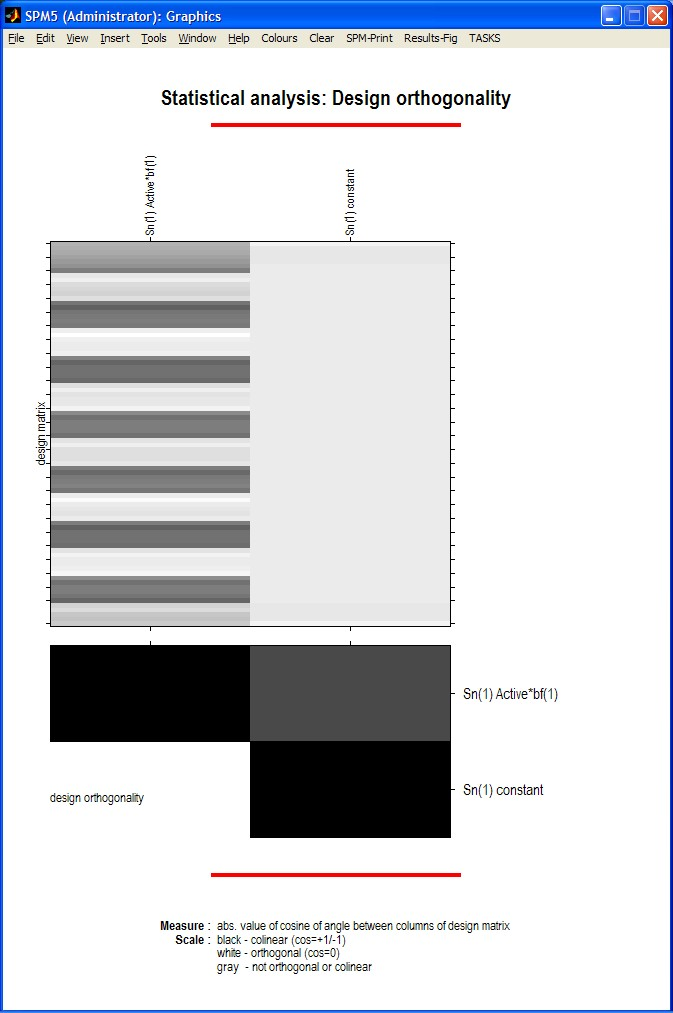
\includegraphics[width=80mm]{auditory/aud_orth}
\caption{\emph{\texttt{Design Orthogonality}: The description above the first column in the design matrix {\sf Sn(1)Active*bf(1)} means that this column refers to the first session of data (in this analysis there is only 1 session), the name of this condition/trial is `Active' and the trial information has been convolved with the first basis function (the canonical hemodynamic response). The constant regressor for session 1 is referred to as {\sf Sn(1)Constant}. The orthogonality matrix at the bottom indicates a degree of collinearity between regressors. \label{aud_orth}}}
\end{center}
\end{figure}

\subsection{Estimate}

Press the \textsc{Estimate} button. This will call up the specification of an fMRI estimation job in the batch editor. Then

\begin{itemize}
\item Highlight the ``Select SPM.mat'' option and then choose the \texttt{SPM.mat} file saved in the classical subdirectory.
\item Save the job as \texttt{estimate.job} and press the \texttt{Run} button.
\end{itemize}

SPM will write a number of files into the selected directory including an \texttt{SPM.mat} file.

\section{Inference}

After estimation:

\begin{itemize}
\item Press ``Results''.
\item Select the \texttt{SPM.mat} file created in the last section.
\end{itemize}

\begin{figure}
\begin{center}
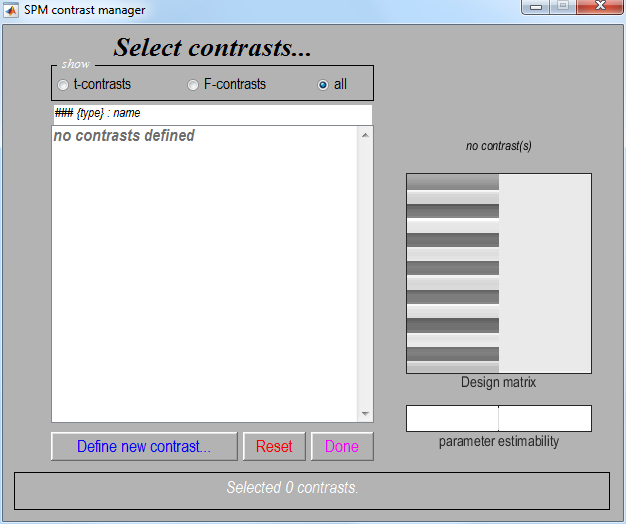
\includegraphics[width=60mm]{auditory/con_man}
\caption{\emph{The contrast manager}}
\end{center}
\end{figure}

This will invoke the contrast manager.

\subsection{Contrast manager}

The contrast manager displays the design matrix (surfable) in the right panel and lists specified contrasts in the left panel. Either ``t-contrast'' or ``F-contrast'' can be selected. To examine statistical results for condition effects

\begin{itemize}
\item{Select ``Define new contrast''}
\end{itemize}
\begin{figure}
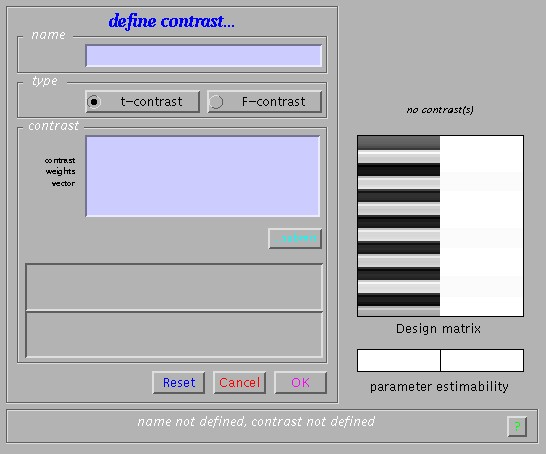
\includegraphics[width=60mm]{auditory/con_man2}
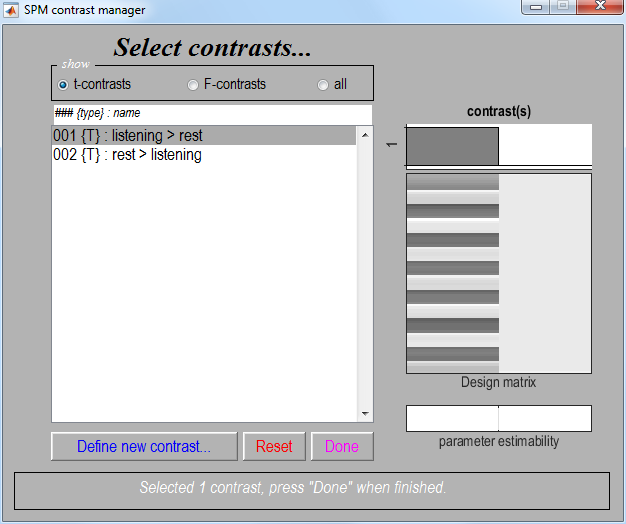
\includegraphics[width=60mm]{auditory/con_man3}
\caption{\emph{Left: A contrast is entered by specifying the numeric values in the lower window and the name in the upper window. Right: After contrasts have been specified they can be selected.}}
\end{figure}

One sided main effects for the active condition (i.e., a one-sided t-test) can be specified (in this example) as ``1'' (active $>$ rest) and ``-1'' (rest $>$ active). SPM will accept correct contrasts only. Accepted contrasts are displayed at the bottom of the contrast manager window in green, incorrect ones are displayed in red. To view a contrast

\begin{itemize}
\item Select the contrast name e.g., ``active $>$ rest''.
\item Press ``Done''.
\end{itemize}

\subsection{Masking}

You will then be prompted with

\begin{itemize}
\item  \emph{Mask with other contrast ? [Yes/No]}.
\item ``Specify No''.
\end{itemize}

Masking implies selecting voxels specified by other contrasts. If ''yes'', SPM will prompt for (one or more) masking contrasts, the significance level of the mask (default p = 0.05 uncorrected), and will ask whether an inclusive or exclusive mask should be used. Exclusive will remove all voxels which reach the default level of significance in the masking contrast, inclusive will remove all voxels which do not reach the default level of significance in the masking contrast. Masking does not affect p-values of the ''target'' contrast, it only includes or excludes voxels.

\subsection{Thresholds}

You will then be prompted with

\begin{itemize}
\item \emph{Title for comparison ?}
\item Enter eg. ``active  $>$ rest''.
\item \emph{p value adjustment to control: [FWE/FDR/none]}.
\item Select ``FWE''.
\item \emph{p value(family-wise error)}.
\item Accept the default value, 0.05.
\end{itemize}

A Family Wise Error (FWE) is a false positive anywhere in the SPM. Now, imagine repeating your experiment many times and producing SPMs. The proportion of SPMs containing FWEs is the FWE rate. A value of 0.05 implies that 1 in 20 SPMs contains a false positive somewhere in the image. 

If you choose the ``none'' option above this corresponds to making statistical inferences at the ``voxel level''. These use ``uncorrected'' p values, whereas FWE thresholds are said to use ``corrected'' p values. SPM's default uncorrected p value is p=0.001. This means that the probability of a false positive at each voxel is 0.001. So if, you have 50,000 voxels you can expect $50,000 \times 0.001 = 50$ false positives in each SPM.

%The final option here is False Discovery Rate (FDR). If you set this at 0.1, this means that of all the discoveries you make (ie. above threshold voxels that appear in the SPM) 10\% of them are likely to be false. 

You will then be prompted with

\begin{itemize}
\item \emph{Extent Threshold \{voxels\} [0]}.
\item Accept the default value, ``0''.
\end{itemize}

Entering a value $v$ here will produce SPMs with clusters containing at least $v$ voxels. SPM will then produce the SPM shown in Figure~\ref{aud_spm1}.

\begin{figure}
\begin{center}
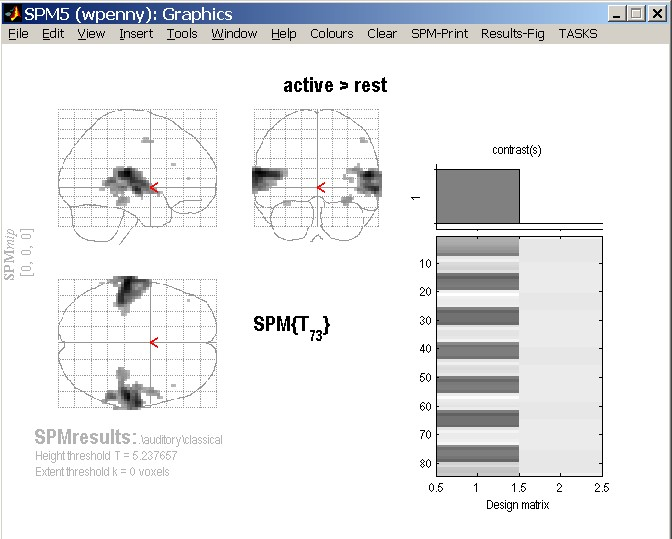
\includegraphics[width=100mm]{auditory/spm1}
\caption{\em SPM showing bilateral activation of auditory cortex. \label{aud_spm1}}
\end{center}
\end{figure}

\subsection{Files}

A number of files are written to the working directory at this time.
Images containing weighted parameter estimates are saved as \texttt{con\_0002.hdr/img}, \texttt{con\_0003.hdr/img}, etc. in the working directory. Images of T-statistics are saved as \texttt{spmT\_0002.hdr/img}, \texttt{spmT\_0003.hdr/img} etc., also in the working directory.

\subsection{Maximum Intensity Projections}

SPM displays a Maximum Intensity Projection (MIP) of the statistical map in the graphics window. The MIP is projected on a glass brain in three orthogonal planes. The MIP is surfable: right-clicking in the MIP will activate a pulldown menu, left-clicking  on the red cursor will allow it to be dragged to a new position.

\begin{figure}
\begin{center}
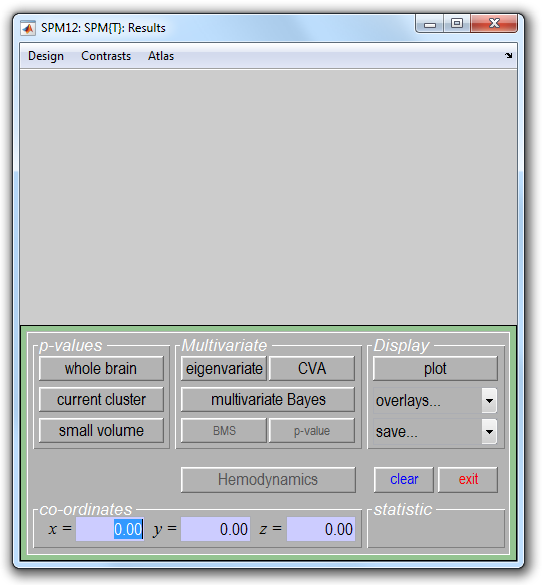
\includegraphics[width=100mm]{auditory/interactive}
\caption{\em SPM's Interactive window during results assessment. The ``p-values'' section is used to produce tables of statistical information. The visualisation section is used to plot responses at a voxel or to visual activations overlaid on anatomical images. The ``Multivariate'' section, ie. the ``eigenvariate'' button, is used to extract data for subsequent analyses such as assessment of PsychoPhysiological Interactions (PPIs) or Dynamic  Causal Models (DCMs).}
\end{center}
\end{figure}

\subsection{Design matrix}

SPM also displays the design matrix with the selected contrast. The design matrix is also surfable: right-clicking will show parameter names, left-clicking will show design matrix values for each scan. 

In the SPM Interactive window (lower left panel) a button box appears with various options for displaying statistical results (p-values panel) and creating plots/overlays (visualisation panel). Clicking ``Design'' (upper left) will activate a pulldown menu as in the ``Explore design'' option.

\subsection{Statistical tables}

To get a summary of local maxima, press the ``whole brain'' button in the p-values section of the interactive window. This will list all clusters above the chosen level of significance as well as separate ($>$8mm apart) maxima within a cluster, with details of significance thresholds and search volume underneath, as shown in Figure~\ref{aud_volume}

\begin{figure}
\begin{center}
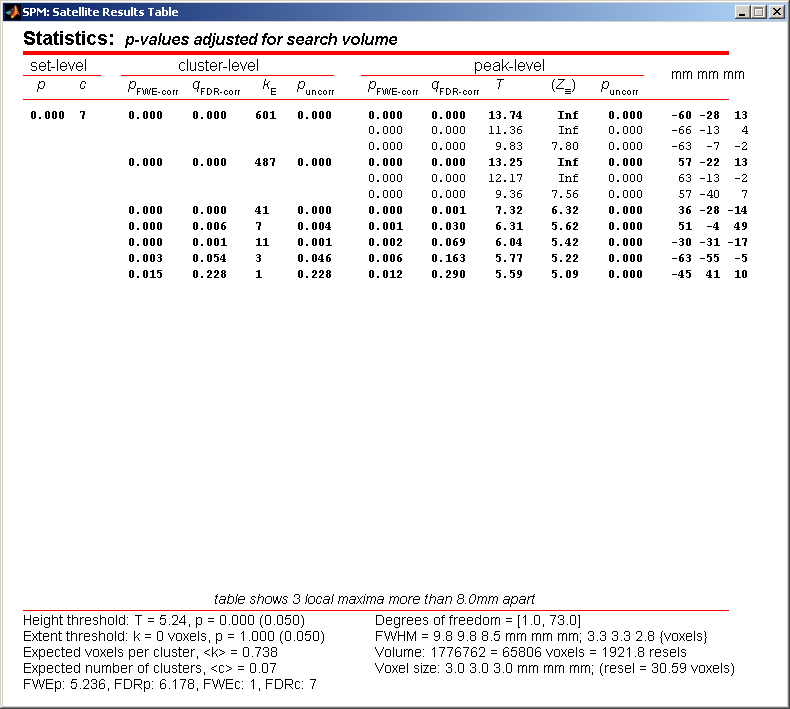
\includegraphics[width=100mm]{auditory/volume}
\caption{\em Volume table for ``active $>$ rest'' effect. This table of values was created by pressing the ``Results-Fig'' tab at the top of the graphics window and then pressing the ``whole brain'' button. This displays the table of results in a separate window. \label{aud_volume}}
\end{center}
\end{figure}

The columns in volume table show, from right to left:

\begin{itemize}
\item \textbf{x, y, z (mm)}: coordinates in MNI space for each maximum.
\item peak-level: the chance (p) of finding (under the null hypothesis) a peak with this or a greater height (T- or Z-statistic), corrected (FWE or FDR)/ uncorrected for search volume.
\item \textbf{cluster-level}: the chance (p) of finding a cluster with this many (ke) or a greater number of voxels, corrected (FWE or FDR)/ uncorrected for search volume.
\item \textbf{set-level}: the chance (p) of finding this (c) or a greater number of clusters in the search volume.
\end{itemize}

It is also worth noting that:

\begin{itemize}
\item The table is surfable: clicking a row of cluster coordinates will move the pointer in the MIP to that cluster, clicking other numbers will display the exact value in the \matlab\ window (e.g. 0.000 = 6.1971e-07).
\item To inspect a specific cluster (e.g., in this example data set, the right auditory cortex), either move the cursor in the MIP (by left-clicking and dragging the cursor, or right-clicking the MIP background which will activate a pulldown menu).
\item Alternatively, click the cluster coordinates in the volume table, or type the coordinates in the co-ordinates section of the interactive window.
\end{itemize}

It is also possible to produce tables of statistical information for a single cluster of interest rather than for the whole volume. Firstly, select the relevant cluster in the MIP and then press the ``current cluster'' button in the p-values section of the interactive window. This will show coordinates and voxel-level statistics for local maxima ($>$4mm apart) in the selected cluster. This table is also surfable.

\subsection{Plotting responses at a voxel}

A voxel can be chosen with co-ordinates corresponding to those in the interactive window. The responses at this voxel can then be plotted using the ``Plot'' button in the visualisation section of the interactive window. This will provide you with five further options:

\begin{enumerate}
\item Contrast estimates and 90\% CI: SPM will prompt for a specific contrast (e.g., active$>$rest). The plot will show effect size and 90\% confidence intervals. See eg. Figure~\ref{aud_contrast}.
\item Fitted responses: Plots adjusted data and fitted response across session/subject. SPM will prompt for a specific contrast and provides the option to choose different ordinates (``an explanatory variable'', ``scan or time'', or ``user specified''). If ``scan or time'', the plot will show adjusted or fitted data with errors added as shown in Figure~\ref{aud_fitted}.
\item Event-related responses: Plots adjusted data and fitted response across peri-stimulus time.
\item Parametric responses.
\item Volterra kernels.
\end{enumerate}

\begin{figure}
\begin{center}
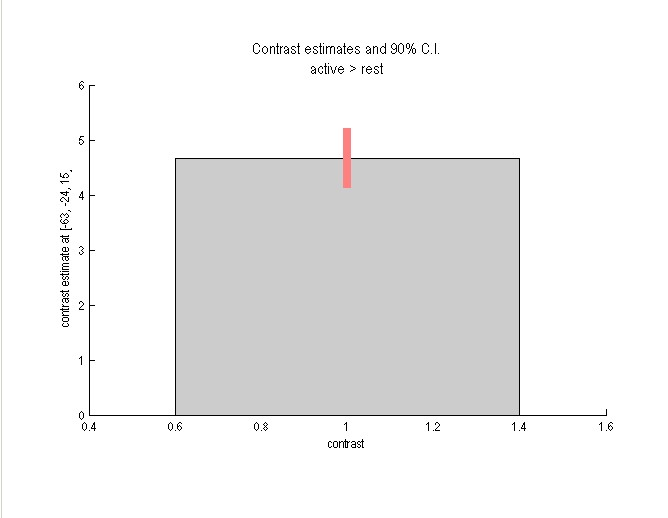
\includegraphics[width=60mm]{auditory/contrast}
\caption{\em Estimated effect size. \label{aud_contrast}}
\end{center}
\end{figure}

\begin{figure}
\begin{center}
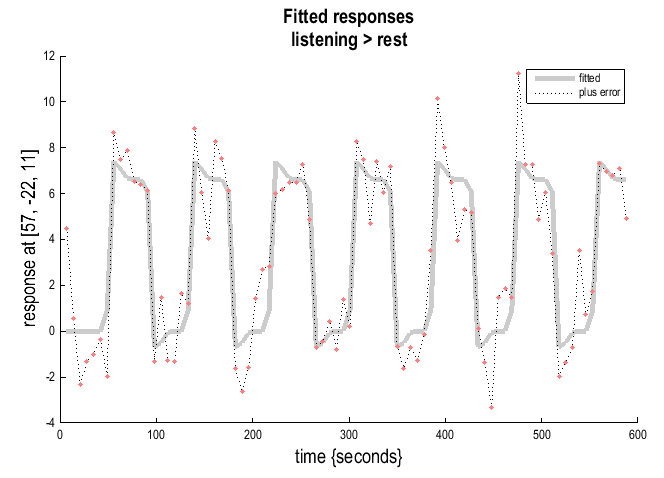
\includegraphics[width=60mm]{auditory/fitted}
\caption{\em Fitted responses. \label{aud_fitted}}
\end{center}
\end{figure}

For plotting event-related responses SPM provides three options

\begin{enumerate}
\item Fitted response and PSTH (peri-stimulus time histogram): plots mean regressor(s) (ie. averaged over session) and mean signal +/- SE for each peri-stimulus time bin.
\item Fitted response and 90\% CI: plots mean regressor(s) along with a 90\% confidence interval.
\item Fitted response and adjusted data: plots regressor(s) and individual data (note that in this example the data are shown in columns due to the fixed TR/ISI relationship).
\end{enumerate}

Its worth noting that

\begin{itemize}
\item The values for the fitted response across session/subject for the selected plot can be displayed and accessed in the Matlab window by typing ``Y''. Typing ``y'' will display the adjusted data.
\item ``Adjusted'' data = adjusted for confounds (e.g., global flow) and high- and low pass filtering.
\end{itemize}

\subsection{Overlays}

The visualisation section of the interactive window also provides an overlay facility for anatomical visualisation of clusters of activation. Pressing ``Overlays'' will activate a pulldown menu with three options

\begin{enumerate}
\item \textbf{Slices}: overlay on three adjacent (2mm) transaxial slices. SPM will prompt for an image for rendering. This could be a canonical image (see \texttt{spm\_template.man}) or an individual T1/mean EPI image for single-subject analyses.
\item \textbf{Sections}: overlay on three intersecting (sagittal, coronal, transaxial) slices. These renderings are surfable: clicking the images will move the crosshair.
\item \textbf{Render}: overlay on a volume rendered brain, with options for using a smoothed brain, and old (left) and new (right) style rendering.
\end{enumerate}

Renderings can be saved as \texttt{filename.img/hdr} in the working directory by using the {\em write filtered} option. In Figures~\ref{aud_slices}, \ref{aud_sections} and \ref{aud_render} the `active $>$ rest' activation has been superimposed on the spatially normalised, bias-corrected anatomical image \texttt{wmsM00223\_002.img} created earlier. 

\begin{figure}
\begin{center}
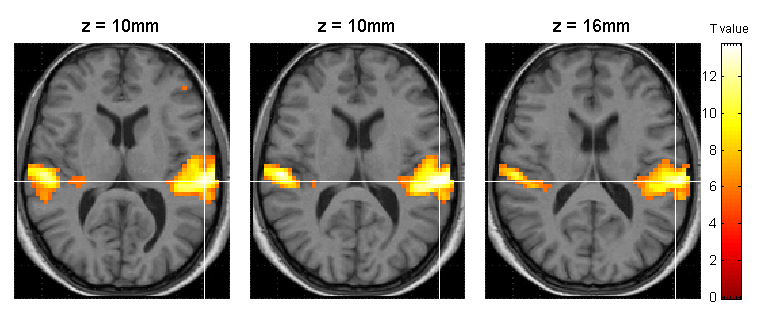
\includegraphics[width=100mm]{auditory/slices}
\caption{\emph{Slices.} \label{aud_slices} }
\end{center}
\end{figure}

\begin{figure}
\begin{center}
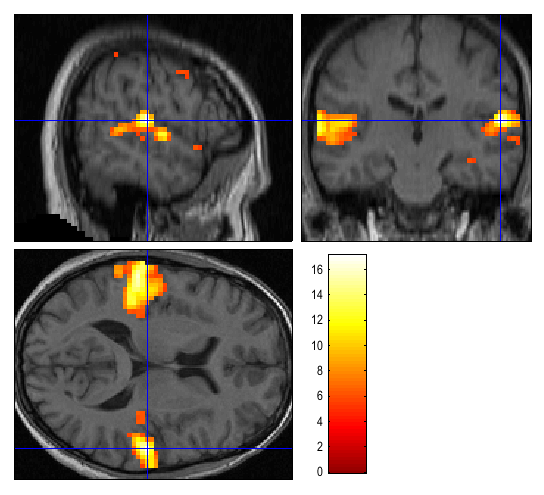
\includegraphics[width=100mm]{auditory/sections}
\caption{\emph{Sections.} \label{aud_sections} }
\end{center}
\end{figure}

For the ``Render'' option we first created a rendering for this subject. This was implemented by 

\begin{itemize}
\item ``Normalise (Write)'' the two images \texttt{c1sM00223\_002.img} and \texttt{c2sM00223\_002.img} using the ``Parameter File '' \texttt{sM00223\_002\_seg\_sn.mat} and a voxel size of [1 1 3].
\item Selecting ``Xtract Surface'' from the ``Render'' pulldown menu.
\item Selecting the gray and white matter images \texttt{wc1sM00223\_002.img} and \texttt{wc2sM00223\_002.img} created in the first step.
\item Saving the results using the default options (Rendering and Surface).
\end{itemize}

SPM plots the rendered anatomical image in the graphics window and saves it as \texttt{render\_wc1sM00223\_002.mat}. The surface image is saved as \texttt{surf\_wc1sM00223\_002.mat}).

\begin{figure}
\begin{center}
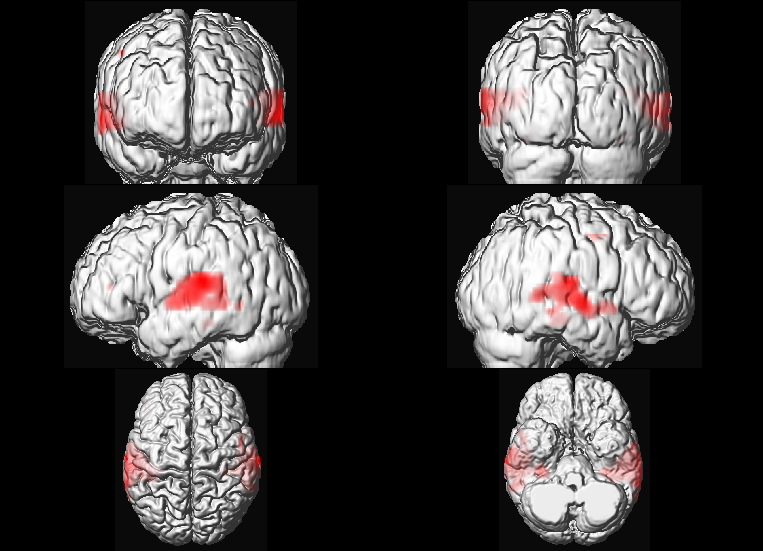
\includegraphics[width=100mm]{auditory/render}
\caption{\emph{Render.} \label{aud_render} }
\end{center}
\end{figure}

\subsection{Miscellaneous}

Other options (in the results controls panel):

\begin{itemize}
\item \textbf{clear}: clears lower subpanel of Graphics window,
\item \textbf{exit}: exits the results section,
\item \textbf{?}: launches help.
\end{itemize}

\section{Bayesian analysis}

\subsection{Specification}

Press the ``Specify 1st-level'' button. This will call up an fMRI specification job in the batch editor. Then

\begin{itemize}
\item Open the fMRI model specification option.
\item Load the ``specify.mat'' job file created for the classical analysis.
\item Open ``Subject/Session'', highlight ``Scans''.
\item Deselect the smoothed functional images using the ``unselect all'' option available from a right mouse click in the SPM file selector (bottom window).
\item Select the unsmoothed functional images using the \texttt{\^w.*} filter and `select all' option available from a right mouse click in the SPM file selector (top right window)\footnote{Remember not to select the first 12 scans, scans 4 to 15, as these may contain T1 effects. This can be done during selection or by first moving the files to a different directory.}. The Bayesian analysis uses a spatial prior where the spatial regularity in the signal is estimated from the data. It is therefore not necessary to create smoothed images if you are only going to do a Bayesian analysis.
\item Press ``Done''.
\item Highlight ``Directory'' and select the \texttt{DIR/bayesian} directory you created earlier (you will first need to deselect the \texttt{DIR/classical} directory).
\item Save the job as \texttt{specify\_bayesian.mat} and press the ``Run'' button.
\end{itemize}

\subsection{Estimation}

Press the ``Estimate'' button. This will call up the specification of an fMRI estimation job in the batch editor. Then

\begin{itemize}
\item Highlight the ``Select SPM.mat'' option and then choose the SPM.mat file saved in the \texttt{DIR/bayesian} directory.
\item Highlight ``Method'' and select the ``Choose Bayesian 1st-level'' option.
\item Open the newly created ``Bayesian 1st-level'' option, highlight ``AR model order'' and select 0. This data set has a TR=7s, so is unlikely to have temporally autocorrelated errors.
\item Save the job as \texttt{estimate\_bayesian.job} and press the ``Run'' butto.
\end{itemize}

SPM will write a number of files into the output directory including 

\begin{itemize}
\item An \texttt{SPM.mat} file.
\item Images of estimated regression coefficients  \texttt{Cbeta\_0001.img} and \texttt{Cbeta\_0002.img}. These filenames are prefixed with a \texttt{C} indicating that these are the mean values of the ``Conditional'' or ``Posterior'' density.
\item Images of error bars/standard deviations on the regression coefficients \texttt{SDbeta\_0001.img} and \texttt{SDbeta\_0002.img}.
\item An image of the standard deviation of the error \texttt{Sess1\_SDerror.img}.
\item An image \texttt{mask.img} indicating which voxels were included in the analysis.
\end{itemize}

\subsection{Inference}

After estimation:

\begin{itemize}
\item Press ``Results'',
\item Select the \texttt{SPM.mat} file created in the last section,
\item Select ``Define new contrast'',
\item Enter the name ``active $>$ rest'',
\item Enter the value ``1'', press ``Submit'', ``OK'', ``Done'',
\item \emph{Mask with other contrast ? [Yes/No]},
\item Specify No,
\item Title for comparison, accept the default,
\item \emph{Effect size threshold for PPM},
\item Enter the value 2,
\item \emph{Posterior probability threshold for PPM},
\item Enter the value 0.99,
\item \emph{Extent threshold [0]},
\item Accept the default value,
\item \emph{Plot effect size [Yes/No]},
\item Select the default `Yes'.
\end{itemize}

SPM will then plot a map of effect sizes at voxels where it is 99\% sure that the effect size is greater than 2\% of the global mean. This is a large activation. Then use overlays, sections, select the normalised structural image created earlier and move the cursor to the activation in the left hemisphere. This should create the plot shown in Figure~\ref{aud_bayes}.

\begin{figure}
\begin{center}
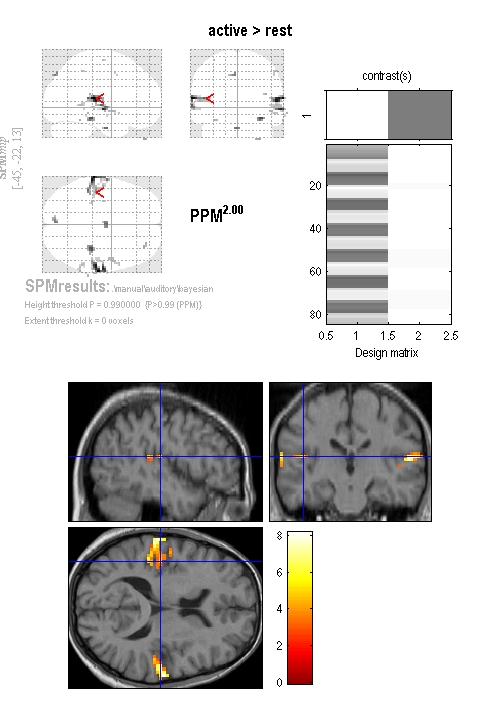
\includegraphics[width=100mm]{auditory/aud_bayes}
\caption{\em \textbf{Bayesian analysis:} MIP and overlay of effect sizes at voxels where SPM is 99\% sure that the effect size is greater than 2\% of the global mean. \label{aud_bayes} }
\end{center}
\end{figure}

It is also possible to look for regions where responses in the active condition are different to those at rest. Active responses could be greater or smaller.

\begin{itemize}
\item Press ``Results'',
\item Select the \texttt{SPM.mat} file created in the last section,
\item Select ``Define new contrast'' and highlight the ``F'' radio button,
\item Enter the name ``active != rest'',
\item Enter the value ``1'', press ``Submit'', ``OK'', ``Done'',
\item \emph{Mask with other contrast ? [Yes/No]},
\item Specify ``No'',
\item Title for comparison, accept the default,
\item \emph{Posterior probability threshold for PPM},
\item Accept the default value\footnote{The default PPM threshold is set to $1-1/S$ where S is the number of voxels in the volume being analysed. The rationale for this is that inference is based on an approximate posterior distribution, $Q$, which factorises across voxels. The approximate posterior is chosen to best match the true posterior in the sense of KL-divergence. Given the factorisation in $Q$, the expected number of false positives in the PPM is 1. },
\item \emph{Extent threshold [0]},
\item Accept the default value, 0,
\item \emph{Plot effect size [Yes/No]},
\item Select the default ``Yes''.
\end{itemize}

SPM will then plot a map of $\chi^2$ statistic values at above threshold voxels. Then use overlays, sections, select the normalised structural image created earlier and move the cursor to the activation in the left hemisphere. This should create the plot shown in Figure~\ref{aud_bayes2}

\begin{figure}
\begin{center}
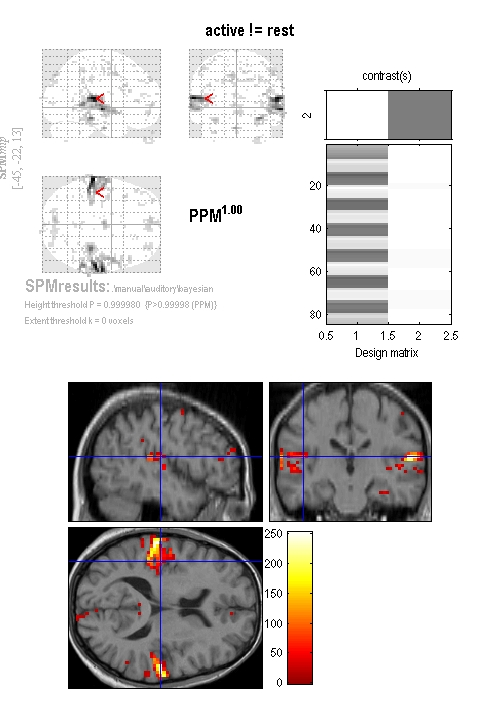
\includegraphics[width=100mm]{auditory/aud_bayes2}
\caption{\em \textbf{Two-sided Bayesian analysis:} MIP and overlay of $\chi^2$ statistic values at above threshold voxels. This shows regions where activity is different between active and rest conditions, whether positive or negative. \label{aud_bayes2} }
\end{center}
\end{figure}

When you revisit the contrast manager this contrast will be referred to as a ``P'' contrast, rather than an ``F'' contrast. This indicates that Bayes rule is used to make the inference. To indicate that we are testing a two-sided effect it is advisable to make this clear when naming the contrast (as we have done with the label ``active != rest'').


\chapter{Face data \label{Chap:data:faces}}

As another, more sophisticated example, consider the data from a repetition priming experiment performed using event-related fMRI.
Briefly, this is a 2$\times$2 factorial study with factors ``fame'' and ``repetition'' where famous and non-famous faces were presented twice against a checkerboard baseline (for more details, see \cite{rnah_face_rep}). The subject was asked to make fame judgements by making key presses. There are thus four event-types of interest; first and second presentations of famous and non-famous faces, which we denote N1, N2, F1 and F2. The experimental stimuli and timings of events are shown in Figures~\ref{face_stim} and \ref{face_timing}.

\begin{figure}
\begin{center}
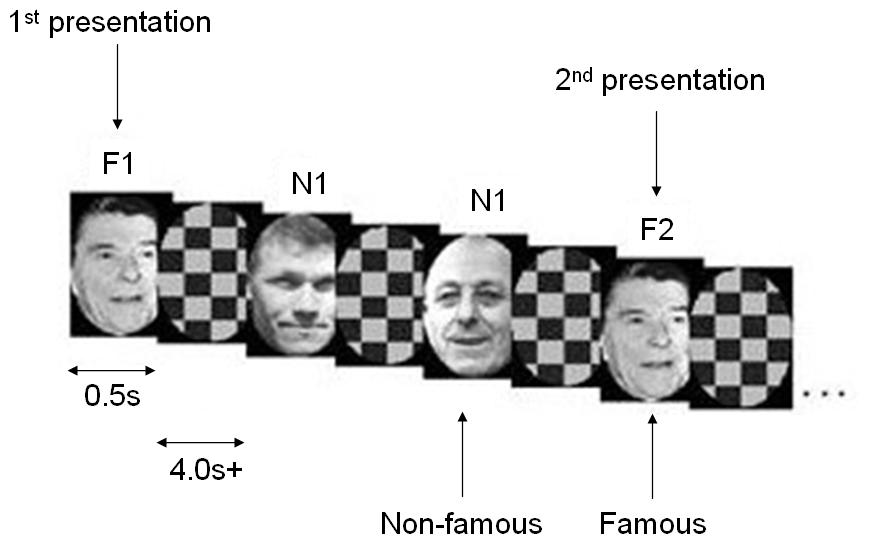
\includegraphics[width=120mm]{faces/face_stim}
\caption{\em \textbf{Face repetition paradigm}: There were 2 presentations of 26 Famous and 26 Nonfamous Greyscale photographs, for 0.5s each, randomly intermixed. The minimal Stimulus Onset Asynchrony (SOA)=4.5s, with probability 2/3 (ie 1/3 null events). The subject made one of two right finger key presses denoting whether or not the subject thought the face was famous. \label{face_stim}}
\end{center}
\end{figure}

\begin{figure}
\begin{center}
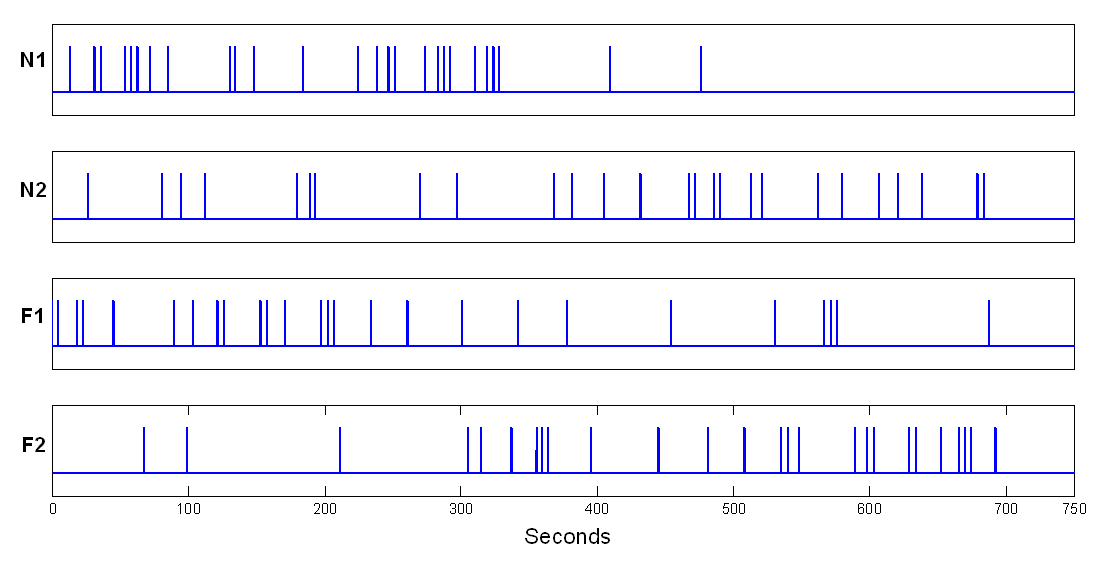
\includegraphics[width=140mm]{faces/face_timing}
\caption{\em Time series of events. \label{face_timing}}
\end{center}
\end{figure}

Images were acquired using continuous Echo-Planar Imaging (EPI) with TE=40ms, TR=2s and 24 descending slices (64$\times$64 3$\times$3 mm$^2$), 3mm thick with a 1.5mm gap.
The data archive is available from the SPM website\footnote{Face Repetition dataset: \url{http://www.fil.ion.ucl.ac.uk/spm/data/face_rep/}}.
This contains 351 Analyze format functional images \texttt{sM03953\_0005\_*.img} of dimension 64$\times$64$\times$24 with 3$\times$3$\times$4.5 mm$^3$ voxels. A structural image is also provided  in Analyze format (\texttt{sM03953\_0007.img}).

To analyse the data, first create a new directory \texttt{DIR} eg. \texttt{C:$\backslash$data$\backslash$face\_rep}, in which to place the results of your analysis. Then create 4 subdirectories (i) \texttt{jobs}, (ii) \texttt{categorical}, (iii)  \texttt{parametric} and (iv) \texttt{bayesian}. As the analysis proceeds these directories will be filled with job-specification files, design matrices and models estimated using classical or Bayesian methods. 

As well as the classical/Bayesian distinction we will show how this data can be analysed from a parametric as well as a categorical perspective. We will look at the 
main effects of fame and repetition and in the parameteric analysis we will look at responses as a function of ``lag'', that is, the number of faces intervening between repetition of a specific face.

Start up matlab, enter your jobs directory and type \texttt{spm fmri} at the \matlab\ prompt. SPM will then open in fMRI mode with three windows (1) the top-left or ``Menu'' window, (2) the bottom-left or ``Interactive'' window and (3) the right-hand or ``Graphics'' window. 
Analysis then takes place in three major stages (i) spatial pre-processing, (ii) model specification, review and estimation and (iii) inference. These stages organise the buttons in SPM's base window.
\begin{figure}
\begin{center}
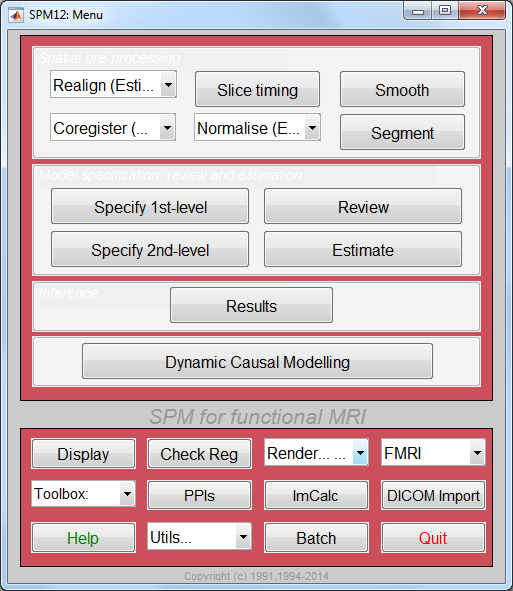
\includegraphics[width=100mm]{faces/command}
\caption{\em The SPM base window comprises three sections (i) spatial pre-processing, (ii) model specification, review and estimation and (iii) inference. \label{command}}
\end{center}
\end{figure}

\section{Spatial pre-processing}

\subsection{Display}

Display eg. the first functional image using the ``Display'' button. Note orbitofrontal and inferior temporal drop-out and ghosting. This can be seen more clearly by selecting ``brighten'' from the ``Effects'' tab in the ``Colours'' at the top of the Graphics window.

\begin{figure}
\begin{center}
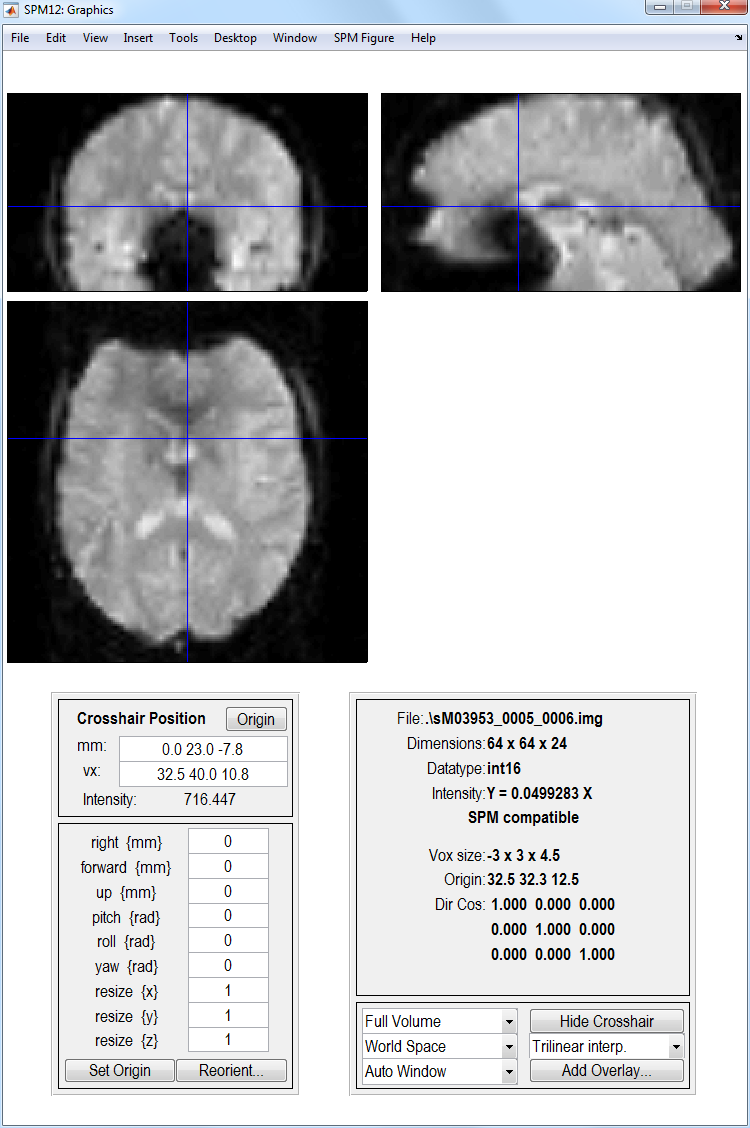
\includegraphics[width=100mm]{faces/dropout}
\caption{\em Signal dropout in EPI images. \label{dropout}}
\end{center}
\end{figure}

\subsection{Realignment}

Under the spatial pre-processing section of the SPM base window select \textsc{Realign (Est \& Res)} from the \textsc{Realign} pulldown menu. This will call up a realignment job specification in the batch editor window.
Then
\begin{itemize}
\item Highlight data, select ``New Session'', then highlight the newly created ``Session'' option.
\item Select ``Specify Files'' and use the SPM file selector to choose all of your functional images eg. \texttt{sM03953\_0005\_*.img}.
\item Save the job file as eg. \texttt{DIR/jobs/realign.mat}.
\item Press the \texttt{Rrn} button in the batch editor window (green triangle).
\end{itemize}
This will run the realign job which will write realigned images into the directory where the functional images are. These new images will be prefixed with the letter ``\texttt{r}''. SPM will then plot the estimated time series of translations and rotations shown in Figure~\ref{face_realign}. These data, the realignment parameters, are also saved to a file eg. \texttt{rp\_sM03953\_0005\_0006.txt}, so that these variables can be used as regressors when fitting GLMs. To prepare for this, copy the file into the \texttt{DIR/jobs} directory and rename it \texttt{movepars.txt}. This allows movements effects to be discounted when looking for brain activations.

SPM will also create a mean image eg. \texttt{meansM03953\_0005\_0006.img} which will be used in the next step of spatial processing - coregistration.
\begin{figure}
\begin{center}
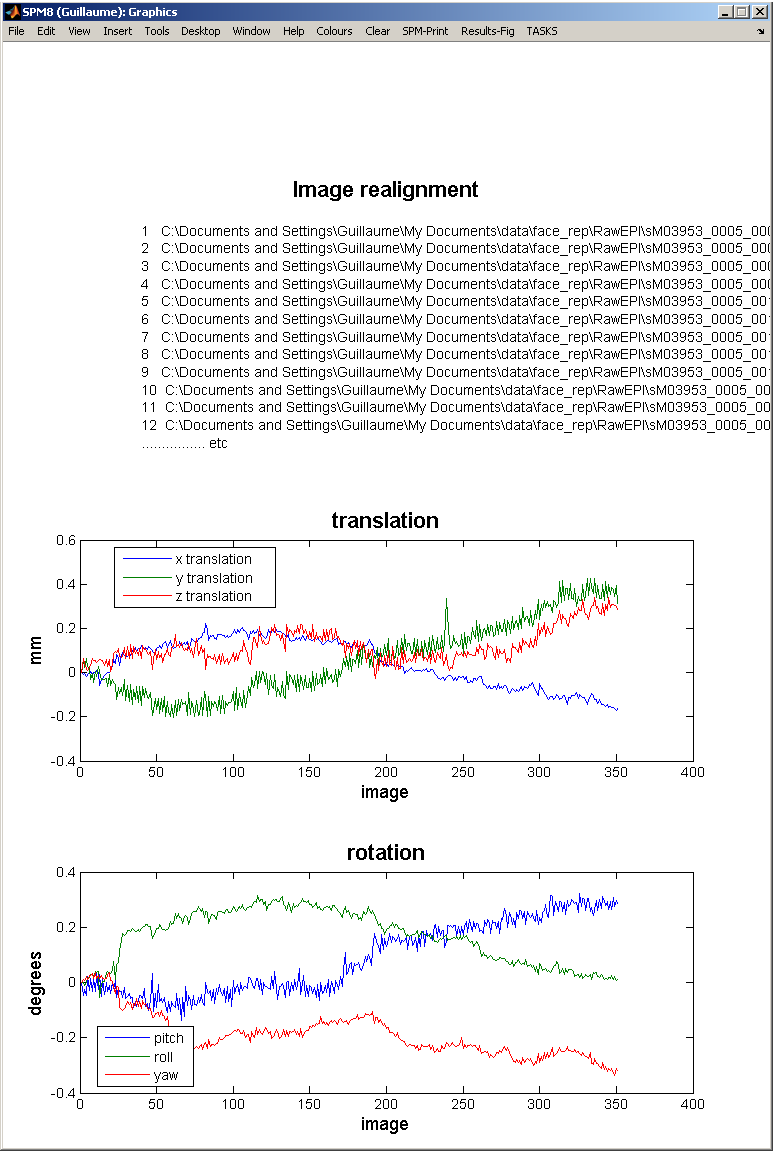
\includegraphics[width=100mm]{faces/realign}
\caption{\em \textbf{Realignment of face data}: Movement less than the size of a voxel, which for this data set is 3mm, is not considered problematic. \label{face_realign}}
\end{center}
\end{figure}

\subsection{Slice timing correction}

Press the textsc{Slice timing} button. This will call up the specification of a slice timing job in the batch editor window. Note that these data consist of N=24 axial slices acquired continuously with a TR=2s (ie TA = TR - TR/N, where TA is the time between the onset of the first and last slice of one volume, and the TR is the time between the onset of the first slice of one volume and the first slice of next volume) and in a descending order (ie, most superior slice was sampled first). The data however are ordered within the file such that the first slice (slice number 1) is the most inferior slice, making the slice acquisition order [24 23 22 ... 1].

\begin{itemize}
\item Highlight ``Data'' and select ``New Sessions''
\item Highlight the newly create ``Sessions'' option, ``Specify Files'' and select the 351 realigned functional images using the filter \texttt{\textasciicircum r.*}.
\item Select ``Number of Slices'' and enter 24.
\item Select TR and enter 2.
\item Select TA and enter 1.92 (or 2 - 2/24).
\item Select ``Slice order'' and enter 24:-1:1.
\item Select ``Reference Slice'', and enter 12.
\item Save the job as \texttt{slice\_timing.mat} and press the ``Run'' button.
\end{itemize}
SPM will write slice-time corrected files with the prefix ``\texttt{a}'' in the functional data directory.

\subsection{Coregistration}

Select \textsc{Coregister (Estimate)} from the \texttt{Coregister} pulldown menu. This will call up the specification of a coregistration job in the batch editor 
window. 

\begin{itemize}
\item Highlight ``Reference Image'' and then select the mean functional image \texttt{meansM03953\_0005\_0006.img}.
\item Highlight ``Source Image'' and then select the structural image eg. \texttt{sM03953\_0007.img}.
\item Press the ``Save'' button and save the job as \texttt{coreg.job}
\item Then press the ``Run'' button.
\end{itemize}

SPM will then implement a coregistration between the structural and functional data that maximises the mutual information. The image in figure~\ref{face_coreg} should then appear in the graphics window. SPM will have changed the header of the source file which in this case is the structural image \texttt{sM03953\_0007.img}.

\begin{figure}
\begin{center}
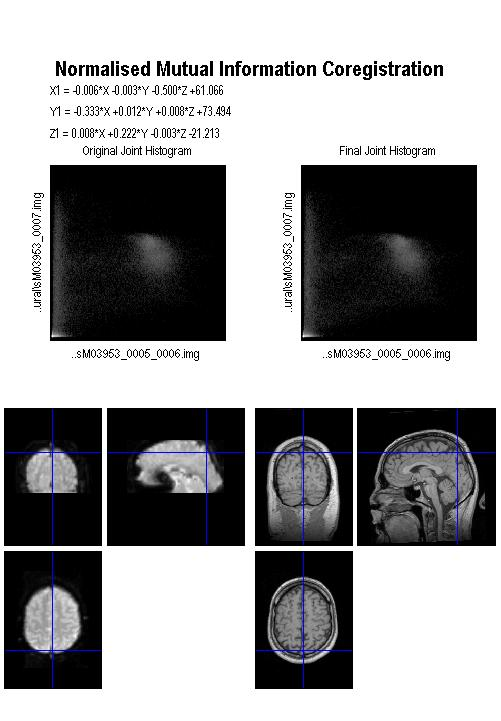
\includegraphics[width=100mm]{faces/coreg}
\caption{\em Mutual Information Coregistration of Face data.\label{face_coreg}}
\end{center}
\end{figure}

\subsection{Segmentation}

Press the \textsc{Segment} button. This will call up the specification of a segmentation job in the batch editor window. Highlight the ``Data'' field and then select the subjects coregistered anatomical image eg. \texttt{sM03953\_0007.img}. Save the job file as \texttt{segment.mat} and then press the \texttt{Run} button. SPM will segment the structural image using the default tissue probability maps as priors. 
SPM will create, by default, gray and white matter images and bias-field corrected structral image. These can be viewed using the CheckReg facility as described in the previous section. Figure~\ref{face_gray} shows the gray matter image, \texttt{c1sM03953\_0007.img}, along with the original structural\footnote{Segmentation can sometimes fail if the source (structural) image is not close in orientation to the MNI templates. It is generally advisable to manually orient the structural to match the template (ie MNI space) as close as possible by using the ``Display'' button, adjusting x/y/z/pitch/roll/yaw, and then pressing the ``Reorient'' button.}.

\begin{figure}
\begin{center}
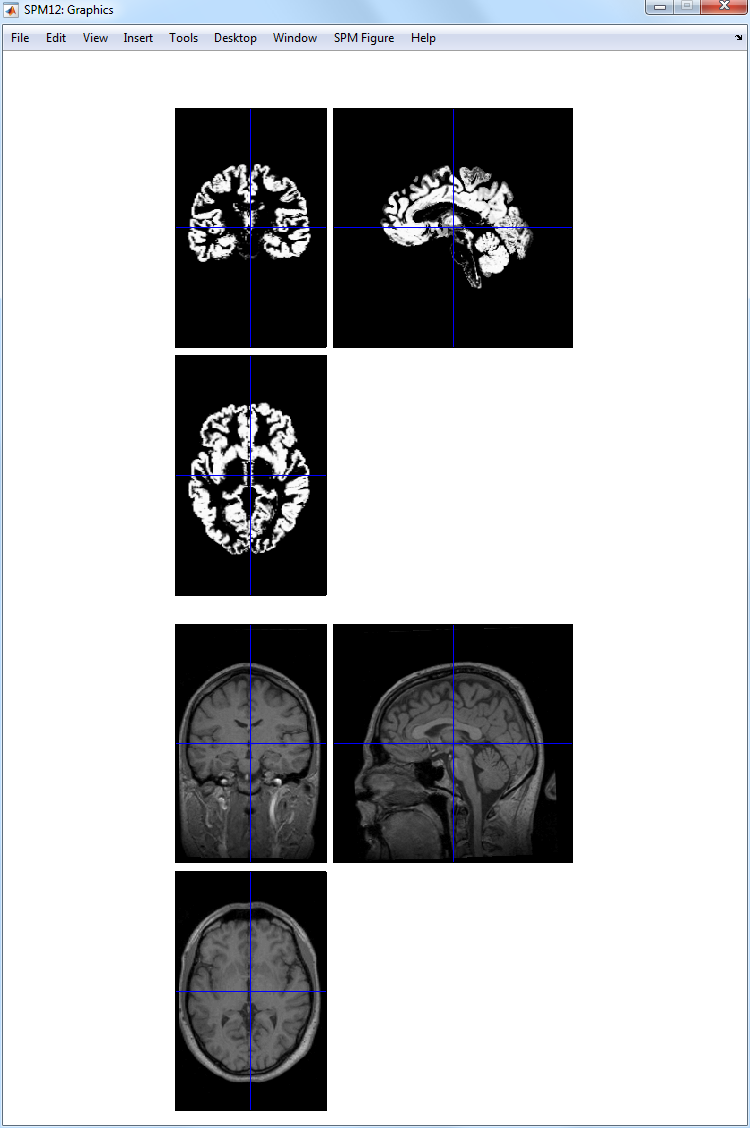
\includegraphics[width=100mm]{faces/gray}
\caption{\em Gray matter (top) produced by segmentation of structural image (below). \label{face_gray}}
\end{center}
\end{figure}

SPM will also write a spatial normalisation eg. \texttt{sM03953\_0007\_seg\_sn.mat} file in the original structural directory. This will be used in the next section to normalise the functional data. 

\subsection{Normalise}

Select \textsc{Normalise (Write)} from the \textsc{Normalise} pulldown menu. This will call up the specification of a normalise job in the batch editor window. 

\begin{itemize}
\item Highlight ``Data'', select ``New Subject''.
\item Open ``Subject'', highlight ``Parameter File'' and select the \texttt{sM03953\_0007\_seg\_sn.mat} file that you created in the previous section.
\item Highlight images to write and select all of the slice-time corrected, realigned functional images \texttt{arsM*.img}. Note: This can be done efficiently by changing the filter in the SPM file selector to \texttt{\textasciicircum ar.*}. You can then right click over the listed files, choose ``Select all''. You might also want to select the mean functional image created during realignment (which would not be affected by slice-time correction), i.e, the \texttt{meansM03953\_0005\_006.img}. Then press ``Done''.
\item Open ``Writing Options'', and change ``Voxel sizes'' from [2 2 2] to [3 3 3]\footnote{This step is not strictly necessary. It will write images out at a resolution closer to that at which they were acquired. This will speed up subsequent analysis and is necessary, for example, to make Bayesian fMRI analysis computationally efficient.}.
\item Press ``Save'', save the job as normalise.mat and then press the \texttt{Run} button.
\end{itemize}
SPM will then write spatially normalised files to the functional data directory. These files have the prefix ``\texttt{w}''.

If you wish to superimpose a subject's functional activations on their own anatomy\footnote{Beginners may wish to skip this step, and instead just superimpose functional activations on an ``canonical structural image''.} you will also need to apply the spatial normalisation parameters to their (bias-corrected) anatomical image. To do this
\begin{itemize}
\item Select \textsc{Normalise (Write)}, highlight `Data', select ``New Subject''.
\item Highlight ``Parameter File'', select the \texttt{sM03953\_0007\_seg\_sn.mat} file that you created in the previous section, press ``Done''.
\item Highlight ``Images to Write'', select the bias-corrected structural eg. \texttt{msM03953\_0007.img}, press ``Done''.
\item Open ``Writing Options'', select voxel sizes and change the default [2 2 2] to [1 1 1] which better matches the original resolution of the images [1 1 1.5].
\item Save the job as \texttt{norm\_struct.mat} and press \texttt{Run} button.
\end{itemize}

\subsection{Smoothing}

Press the \textsc{Smooth} button\footnote{The smoothing step is unnecessary if you are only interested in Bayesian analysis of your functional data.}. This will call up the specification of a smooth job in the batch editor window.

\begin{itemize}
\item Select ``Images to Smooth'' and then select the spatially normalised files created in the last section eg. \texttt{war*.img}.
\item Save the job as {\sf smooth.mat} and press \texttt{Run} button.
\end{itemize}

This will smooth the data by (the default) 8mm in each direction, the default smoothing kernel width.

\begin{figure}
\begin{center}
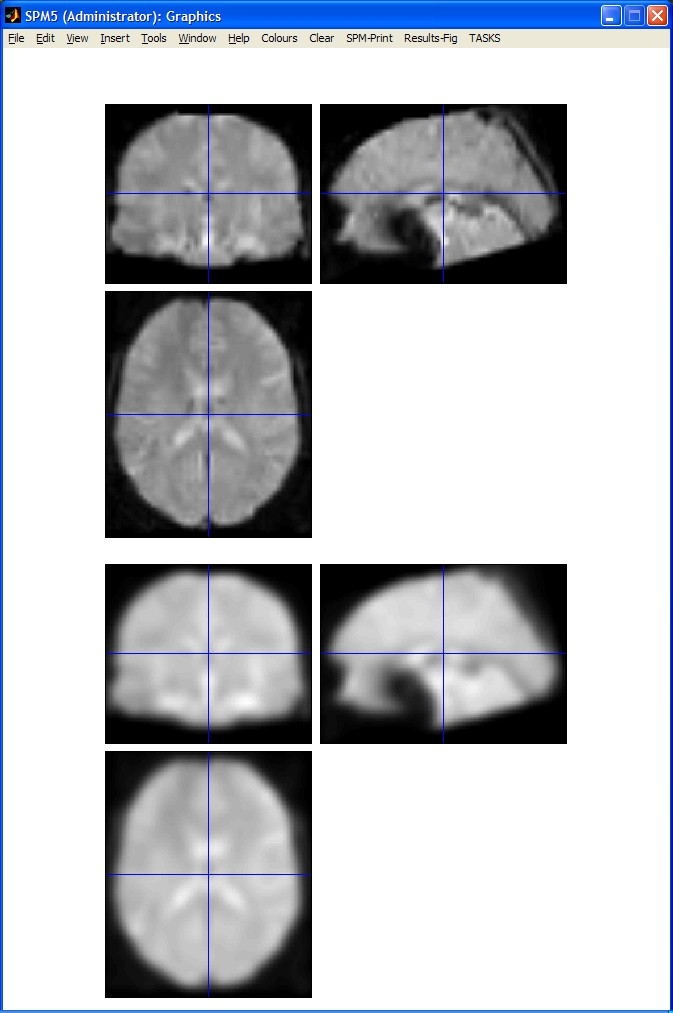
\includegraphics[width=100mm]{faces/smooth}
\caption{\em Functional image (top) and 8mm-smoothed functional image (bottom). These images were plotted using SPM's ``CheckReg'' facility. \label{face_smooth}}
\end{center}
\end{figure}

\section{Modelling categorical responses}

Before setting up the design matrix we must first load the Stimulus Onsets Times (SOTs) and movement parameters into matlab. SOTs are stored in the \texttt{sots.mat} file in a cell array such that eg. \texttt{sot\{1\}} contains stimulus onset times in TRs for event type 1, which is N1. Event-types 2, 3 and 4 are N2, F1 and F2.\footnote{Unlike previous analyses of these data in SPM99 and SPM2, we will not bother with extra event-types for the (rare) error trials.}
\begin{itemize}
\item At the \matlab\ command prompt type \texttt{load sots}
\item Then type \texttt{load movepars.txt}
\end{itemize}

Now press the \textsc{Specify 1st-level} button. This will call up the specification of a fMRI specification job in the batch editor window. Then

\begin{itemize}
\item In the ``Timing paramaters'' option,
\item Highlight ``Units for design'' and select ``Scans'',
\item Highlight ``Interscan interval'' and enter 2,
\item Highlight ``Microtime resolution'' and enter 24,
\item Highlight ``Microtime onset'' and enter 12. These last two options make the creating of regressors commensurate with the slice-time correction we have applied to the data, given that there are 24 slices and that the reference slice to which the data were slice-time corrected was the 12th (middle slice in time).
\item Highlight ``Data and Design'' and select ``New Subject/Session''.
\item Highlight ``Scans'' and use SPM's file selector to choose the 351 smoothed, normalised, slice-time corrected, realigned functional images ie \texttt{swarsM.img}. These can be selected easily using the \texttt{\textasciicircum swar.*} filter, and select all. Then press ``Done''.
\item Highlight ``Conditions'' and select ``New condition''\footnote{It is also possible to enter information about all of the conditions in one go. This requires much less button pressing and can be implemented by highlighting the ``Multiple conditions'' option and then selecting the \texttt{all-conditions.mat} file, which is also provided on the webpage.}.
\item Open the newly created ``Condition'' option. Highlight ``Name'' and enter ``N1''. Highlight ``Onsets'' and enter \texttt{sot\{1\}}. Highlight ``Durations'' and enter 0.
\item Highlight ``Conditions'' and select ``Replicate condition''.
\item Open the newly created ``Condition'' option (the lowest one). Highlight ``Name'' and change to ``N2''. Highlight ``Onsets'' and enter \texttt{sot\{2\}}.
\item Highlight ``Conditions'' and select ``Replicate condition''.
\item Open the newly created ``Condition'' option (the lowest one). Highlight ``Name'' and change to ``F1''. Highlight ``Onsets'' and enter \texttt{sot\{3\}}.
\item Highlight ``Conditions'' and select ``Replicate condition''.
\item Open the newly created ``Condition'' option (the lowest one). Highlight ``Name'' and change to ``F2''. Highlight ``Onsets'' and enter \texttt{sot\{4\}}.
\item Highlight ``Multiple Regressors'' and select the \texttt{movepars.txt} file\footnote{It is also possible to enter regressors one by one by highlighting ``Regressors'' and selecting ``New Regressor'' for each one. Here, we benefit from the fact that the realignment stage produced a text file with the correct number of rows (351) and columns (6) for SPM to add 6 regressors to model (linear) rigid-body movement effects.}.
\item Highlight ``Factorial Design'', select ``New Factor'', open the newly created ``Factor'' option, highlight ``Name'' and enter ``Fam'', highlight ``Levels'' and enter 2.
\item Highlight ``Factorial Design'', select ``New Factor'', open the newly created ``Factor'' option, highlight ``Name'' and enter ``Rep'', highlight ``Levels'' and enter 2\footnote{The order of naming these factors is important - the factor to be specified first is the one that ``changes slowest'' ie. as we go through the list of conditions N1, N2, F1, F2 the factor ``repetition'' changes every condition and the factor ``fame'' changes every other condition. So ``Fam'' changes slowest and is entered first.}.
\item Open ``Canonical HRF'' under ``Basis Functions''. Select ``Model derivatives'' and select ``Time and Dispersion derivatives''.
\item Highlight ``Directory'' and select the \texttt{DIR/categorical} directory you created earlier.
\item Save the job as \texttt{categorical\_spec.mat} and press the \texttt{Run} button.
\end{itemize}

SPM will then write an \texttt{SPM.mat} file to the \texttt{DIR/categorical} directory. It will also plot the design matrix, as shown in Figure~\ref{cat_design}. 
\begin{figure}
\begin{center}
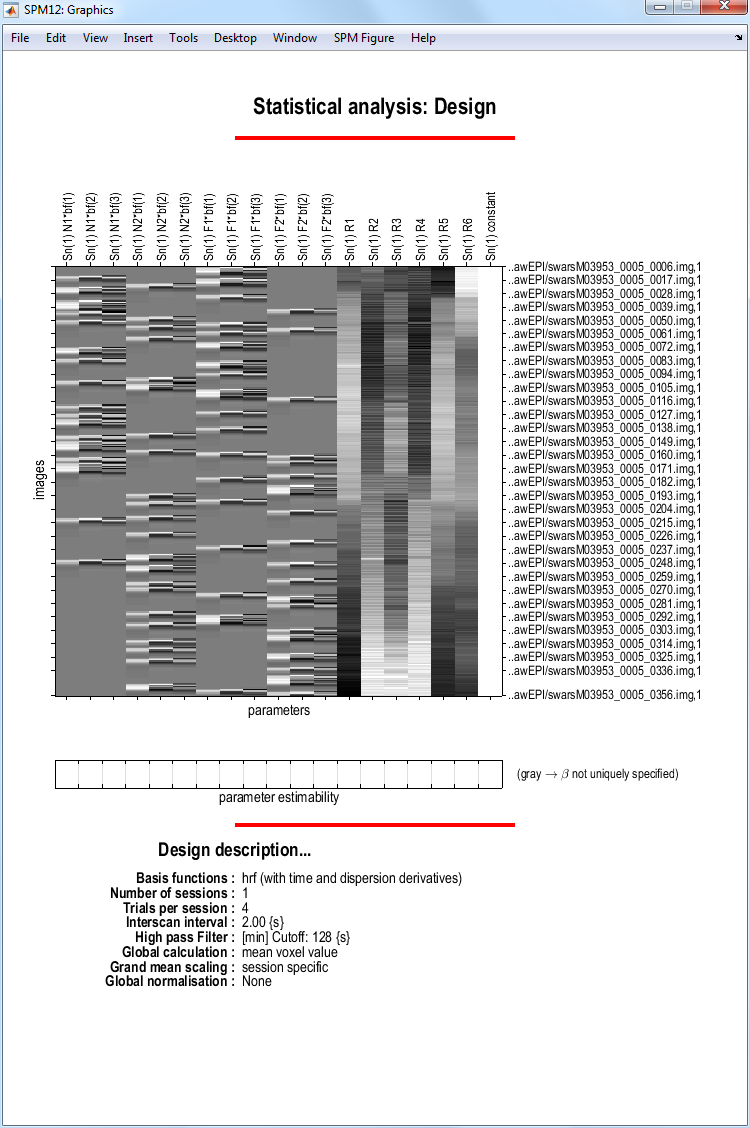
\includegraphics[width=100mm]{faces/cat_design}
\caption{\em \textbf{Design matrix}. \label{cat_design}}
\end{center}
\end{figure}

At this stage it is advisable to check your model specification using SPM's review facility which is accessed via the ``Review'' button. This brings up a ``design'' tab on the interactive window clicking on which produces a pulldown menu. If you select the first item ``Design Matrix'' SPM will produce the image shown in Figure~\ref{cat_design}. If you select ``Explore'' then ``Session 1'' then ``N1'', SPM will produce the plots shown in Figure~\ref{cat_explore}.
\begin{figure}
\begin{center}
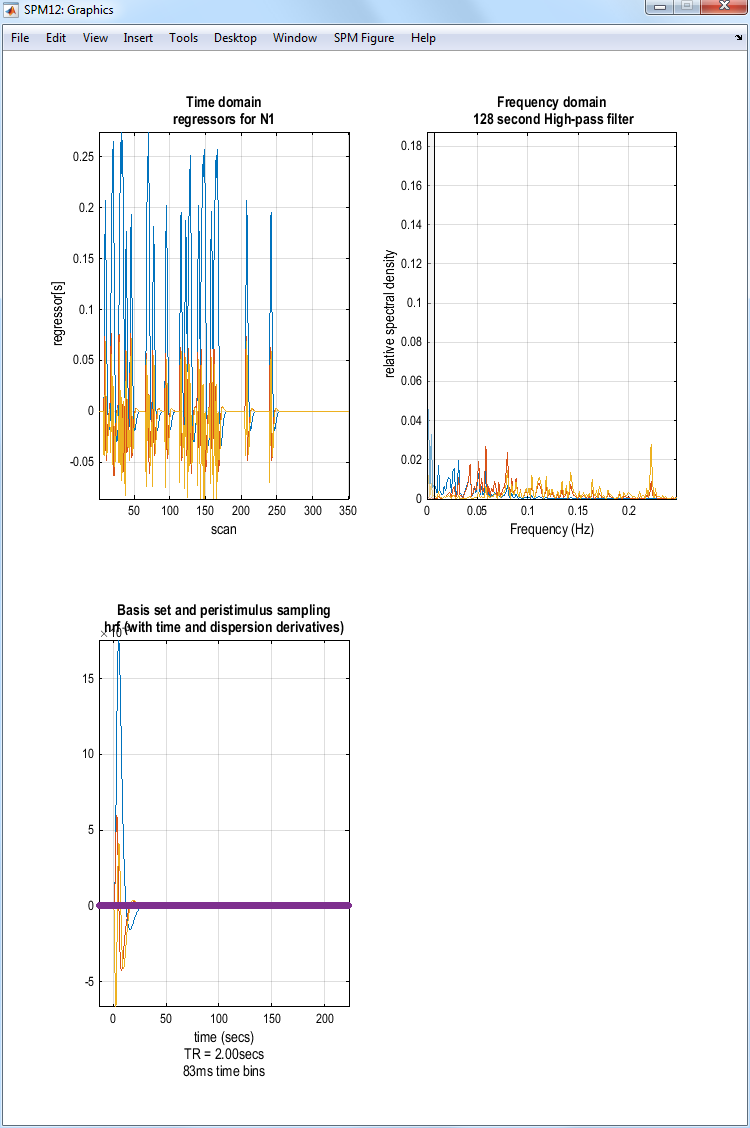
\includegraphics[width=100mm]{faces/cat_explore}
\caption{\em \textbf{Exploring the design matrix in Figure~\ref{cat_design}}. This shows the time series of the ``N1'' regressor (top left), the three basis functions used to convert assumed neuronal activity into hemodynamic activity (bottom left), and a frequency domain plot of the three regressors for the basis functions in this condition (top right). The frequency domain plot shows that the frequency content of the ``N1'' condition is generally above the set frequencies that are removed by the High Pass Filter (HPF) (these are shown in gray - in this model we accepted the default HPF cut-off of 128s or 0.008Hz). \label{cat_explore}}
\end{center}
\end{figure}

\subsection{Estimate}

Press the \textsc{Estimate} button. This will call up the specification of an fMRI estimation job in the batch editor window. Then
\begin{itemize}
\item Highlight the ``Select SPM.mat'' option and then choose the \texttt{SPM.mat} file saved in the \texttt{DIR/categorical} directory.
\item Save the job as \texttt{categorical\_est.job} and press \texttt{Run} button.
\end{itemize}
SPM will write a number of files into the selected directory including an \texttt{SPM.mat} file.

\subsection{Inference for categorical design}

Press ``Results'' and select the SPM.mat file from \texttt{DIR/categorical}. This will again invoke the contrast manager. Because we specified that our model was using a ``Factorial design'' a number of contrasts have been specified automatically, as shown in Figure~\ref{cat_contrasts}.
\begin{figure}
\begin{center}
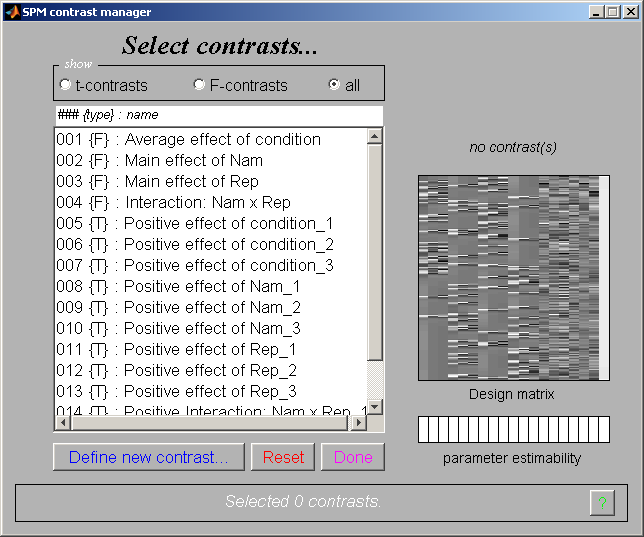
\includegraphics[width=100mm]{faces/cat_contrasts}
\caption{\em Contrast Manager containing default contrasts for categorical design. \label{cat_contrasts}}
\end{center}
\end{figure}

\begin{itemize}
\item Select contrast number 5. This is a t-contrast \texttt{Positive effect of condition\_1} This will show regions where the average effect of presenting faces is significantly positive, as modelled by the first regressor (hence the \texttt{\_1}), the canonical HRF. Press `Done''.
\item \emph{Mask with other contrast ? [Yes/No]}
\item Specify No.
\item \emph{Title for comparison ?}
\item Enter ``Canonical HRF: Faces $>$ Baseline''
\item \emph{p value adjustment to control: [FWE/FDR/none]}
\item Select FWE
\item \emph{Corrected p value(family-wise error)}
\item Accept the default value, 0.05
\item \emph{Extent threshold \{voxels\} [0]}
\item Accept the default value, 0.
\end{itemize}
SPM will then produce the MIP shown in Figure~\ref{cat5_volume}.

\subsection{Statistical tables}

To get a summary of local maxima, press the ``whole brain'' button in the p-values section of the interactive window. This will list all clusters above the chosen level of significance as well as separate ($>$8mm apart) maxima within a cluster, with details of significance thresholds and search volume underneath, as shown in Figure~\ref{cat5_volume}
\begin{figure}
\begin{center}
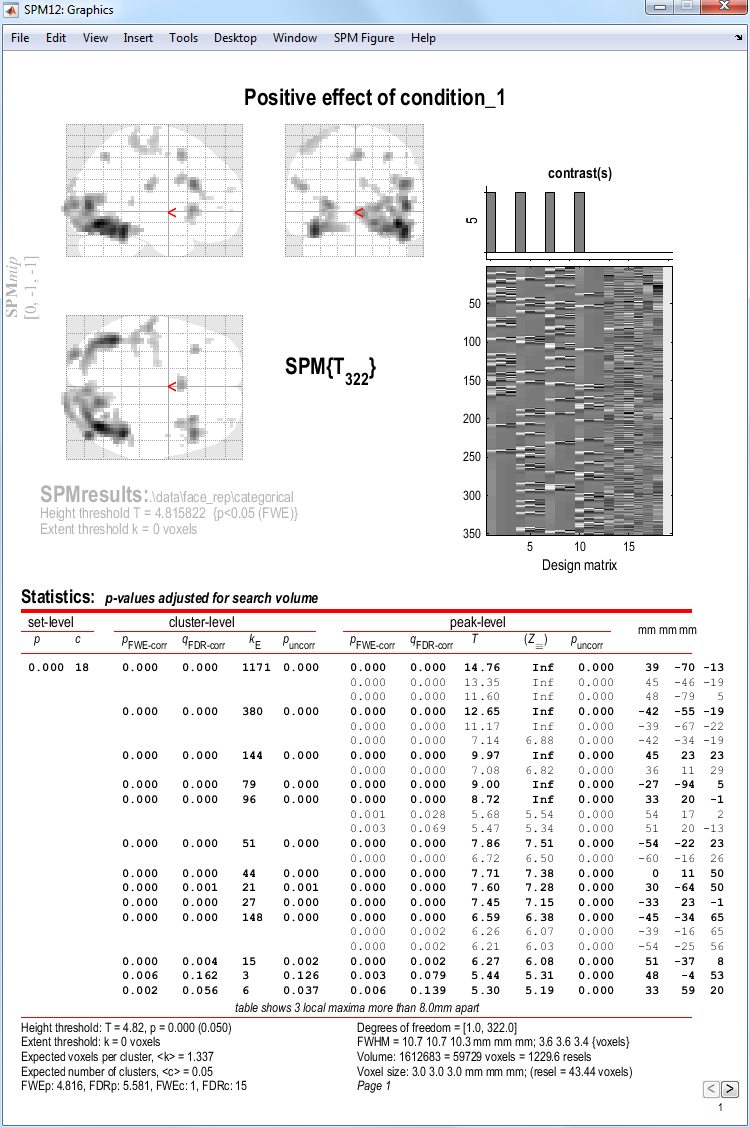
\includegraphics[width=100mm]{faces/cat5_volume}
\caption{\em \textbf{MIP and Volume table for Canonical HRF}: Faces  $>$ Baseline. \label{cat5_volume} }
\end{center}
\end{figure}

The columns in volume table show, from right to left:
\begin{itemize}
\item \textbf{x, y, z (mm)}: coordinates in MNI space for each maximum.
\item \textbf{peak-level}: the chance (p) of finding (under the null hypothesis) a peak with this or a greater height (T- or Z-statistic), corrected (FWE or FDR)/ uncorrected for search volume.
\item \textbf{cluster-level}: the chance (p) of finding a cluster with this many(ke) or a greater number of voxels, corrected (FWE or FDR)/ uncorrected for search volume.
\item \textbf{set-level}: the chance (p) of finding this (c) or a greater number of clusters in the search volume.
\end{itemize}

Right-click on the MIP and select ``goto global maximum''. The cursor will move to [39 -70 -14]. You can view this activation on the subject's normalised, attenuation-corrected structural (\texttt{wmsM03953\_0007\.img}), which gives best anatomical precision, or on the normalised mean functional (\texttt{wmeansM03953\_0005\_0006.img}), which is closer to the true data and spatial resolution (including distortions in the functional EPI data). 

If you select ``plot'' and choose ``Contrast of estimates and 90\% C.I'' (confidence interval), and select the ``Average effect of condition'' contrast, you will see three bars corresponding to the parameter estimates for each basis function (summed across the 4 conditions). The BOLD impulse response in this voxel loads mainly on the canonical HRF, but also significantly (given that the error bars do not overlap zero) on the temporal and dispersion derivatives (see next Chapter).

\subsection{F-contrasts}

To assess the main effect of repeating faces, as characterised by both the hrf \emph{and} its derivatives, an F-contrats is required. This is really asking whether repetition changes the \emph{shape} of the impulse response (e.g, it might affect its latency but not peak amplitude), at least the range of shapes defined by the three basis functions. Because we have told SPM that we have a factorial design, this required contrast will have been created automatically - it is number 3. 

\begin{itemize}
\item Press ``Results'' and select the \texttt{SPM.mat} file in the \texttt{DIR/categorical} directory.
\item Select the ``F-contrast'' toggle and the contrast number 3, as shown in Figure~\ref{cat3_contrast}. Press ``Done''.
\item \emph{Mask with other contrast ? [Yes/No]}.
\item Specify ``Yes''.
\item Select contrast 5 - \texttt{Positive effect of condition\_1} (the T-contrast of activation versus baseline, collapsed across conditions, that we evaluated above)
\item \emph{uncorrected mask p-value ?}
\item Change to 0.001
\item \emph{nature of mask?}
\item Select 'inclusive'
\item \emph{Title for comparison ?}
\item Keep ``Main effect of Rep (masked with ...)''
\item \emph{p value adjustment to control: [FWE/none]}
\item Select none
\item \emph{threshold (F or p value)}
\item Accept the default value, 0.001
\item \emph{Extent threshold \{voxels\} [0]}
\item Accept the default value, 0
\end{itemize}

A MIP should then appear, the top half of which should look like Figure~\ref{cat3_psth}.

\begin{figure}
\begin{center}
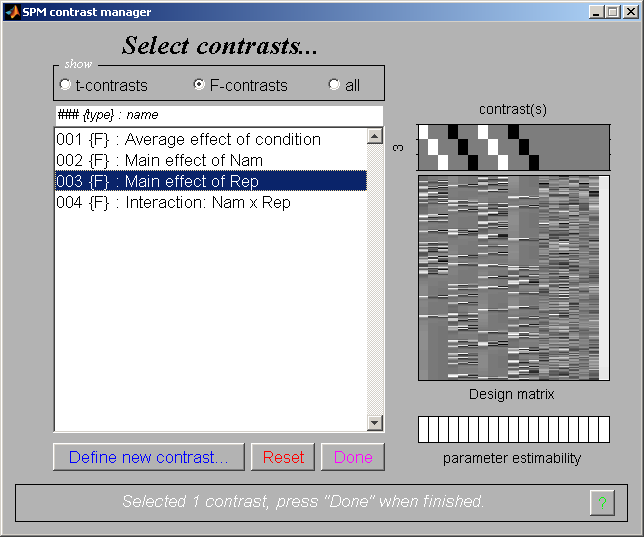
\includegraphics[width=100mm]{faces/cat3_contrast}
\caption{\em Contrast manager showing selection of the first contrast ``Main effect of Rep'' (repetition: F1 and N1 vs F2 and N2)\label{cat3_contrast} }
\end{center}
\end{figure}

\begin{figure}
\begin{center}
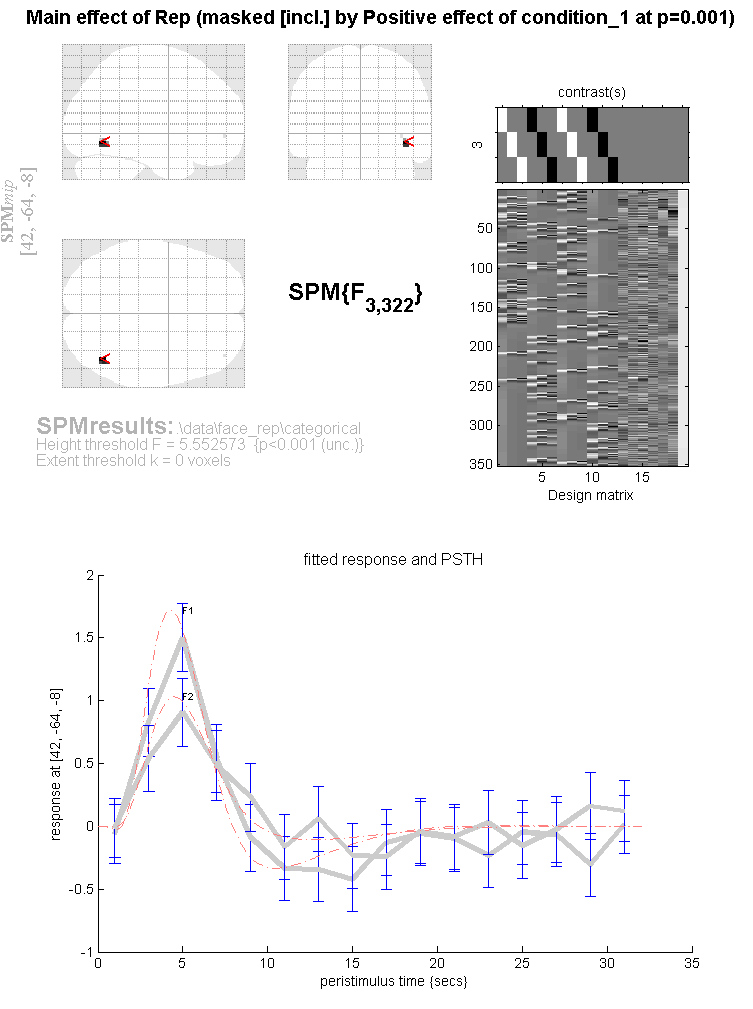
\includegraphics[width=100mm]{faces/cat3_psth}
\caption{\em MIP for Main effect of Rep, masked inclusively with Canonical HRF: Faces  $>$ Baseline at p$<$.001 uncorrected. Shown below are the best-fitting responses and peri-stimulus histograms (PSTH) for F1 and F2. \label{cat3_psth} } 
\end{center}
\end{figure}

Note that this contrast will identify regions showing any effect of repetition (e.g, decreased or increased amplitudes) \emph{within} those regions showing activations (on the canonical HRF) to faces versus baseline (at p$<$.05 uncorrected). Select ``goto global max'', which is in right ventral temporal cortex [42 -64 -8].

If you press plot and select ``Event-related responses'', then ``F1'', then ``fitted response and PSTH'', you will see the best fitting linear combination of the canonical HRF and its two derivatives (thin red line), plus the ``selectively-averaged'' data (peri-stimulus histogram, PSTH), based on an FIR refit (see next Chapter). 
If you then select the ``hold'' button on the Interactive window, and then ``plot'' and repeat the above process for the ``F2'' rather than ``F1'' condition, you will see two estimated event-related responses, in which repetition decreases the peak response (ie F2$<$F1), as shown in Figure~\ref{cat3_psth}.

You can explore further F-contrasts, which are a powerful tool once you understand them. For example, the MIP produced by the ``Average effect of condition'' F-contrast looks similar to the earlier T-contrast, but importantly shows the areas for which the sums across conditions of the parameter estimates for the canonical hrf \emph{and/or} its temporal derivative \emph{and/or} its dispersion derivative are different from zero (baseline). The first row of this F-contrast ([1 0 0 1 0 0 1 0 0 1 0 0]) is also a two-tailed version of the above T-contrast, ie testing for both activations and deactivations versus baseline. This also means that the F-contrasts [1 0 0 1 0 0 1 0 0 1 0 0] and [-1 0 0 -1 0 0 -1 0 0 -1 0 0] are equivalent. Finally, note that an F- (or t-) contrast such as [1 1 1 1 1 1 1 1 1 1 1], which tests whether the mean of the canonical hrf AND its derivatives for all conditions are different from (larger than) zero is not sensible. This is because the canonical hrf and its temporal derivative may cancel each other out while being significant in their own right. The basis functions are really quite different things, and need to represent separate rows in an F-contrast. 

\subsection{F-contrasts for testing effects of movement}

To assess movement-related activation
\begin{itemize}
\item Press ``Results'', select the \texttt{SPM.mat} file, select ``F-contrast'' in the Contrast Manager. Specify e.g. ``Movement-related effects'' (name) and 
in the ``contrasts weights matrix'' window, or ``1:12 19'' in the ``columns for reduced design'' window.
\item Submit and select the contrast, specify ``mask with other contrasts?'' (no), ``title for comparison'' (accept default), ``corrected height threshold'' (FWE), and ``corrected p-value'' (accept default). 
\item When the MIP appears, select ``sections'' from the ``overlays'' pulldown menu, and select the normalised structural image (\texttt{wmsM03953\_0007.img}).
\end{itemize}

You will see there is a lot of residual movement-related artifact in the data (despite spatial realignment), which tends to be concentrated near the boundaries of tissue types (eg the edge of the brain; see Figure~\ref{movements}). (Note how the MIP can be misleading in this respect, since though it appears that the whole brain is affected, this reflects the nature of the (X-ray like) projections onto each orthogonal view; displaying the same datae as sections in 3D shows that not every voxel is suprathreshold.)  Even though we are not interested in such artifact, by including the realignment parameters in our design matrix, we ``covary out'' (linear components) of subject movement, reducing the residual error, and hence improve our statistics for the effects of interest.

\begin{figure}
\begin{center}
\includegraphics[width=100mm]{faces/movements}
\caption{\em Movement-related activations. These spurious `activations' are due to residual movement of the head during scanning. These effects occur at tissue boundaries and boundaries between brain and non-brain, as this is where contrast differences are greatest. Including these regressors in the design matrix means these effects cannot be falsely attributed 
to neuronal activity. \label{movements} }
\end{center}
\end{figure}

\section{Modelling parametric responses}

Before setting up the design matrix, we must first load into \matlab\ the Stimulus Onsets Times (SOTs), as before, and also the ``Lags'', which are specific to this experiment, and which will be used as parametric modulators. The Lags code, for each second presentation of a face (N2 and F2), the number of other faces intervening between this (repeated) presentation and its previous (first) presentation. Both SOTs and Lags are represented by Matlab cell arrays, stored in the \texttt{sots.mat} file.

\begin{itemize}
\item At the \matlab\ command prompt type \texttt{load sot}. This loads the stimulus onset times and the lags (the latter in a cell array called \texttt{itemlag}.
\end{itemize}

Now press the \textsc{Specify 1st-level} button. This will call up the specification of a fMRI specification job in the batch editor window. Then
\begin{itemize}
\item Press ``Load'' and select the \texttt{categorical\_spec.mat} job file you created earlier.
\item Open ``Conditions'' and then open the second ``Condition''.
\item Highlight ``Parametric Modulations'', select ``New Parameter''.
\item Highlight ``Name'' and enter ``Lag'', highlight values and enter \texttt{itemlag\{2\}}, highlight polynomial expansion and ``2nd order''.
\item Now open the fourth ``Condition'' under ``Conditions''.
\item Highlight ``Parametric Modulations'', select ``New Parameter''.
\item Highlight ``Name'' and enter ``Lag'', highlight values and enter \texttt{itemlag\{4\}}, highlight polynomial expansion and ``2nd order''.
\item Open ``Canonical HRF'' under ``Basis Functions'', highlight ``Model derivatives'' and select ``No derivatives'' (to make the design matrix a bit simpler for present purposes!).
\item Highlight ``Directory'' and select \texttt{DIR/parametric} (having ``unselected'' the current definition of directory from the Categorical analysis).
\item Save the job as \texttt{parametric\_spec} and press the \texttt{Run} button.
\end{itemize}

This should produce the design matrix shown in Figure~\ref{par_design}.

\begin{figure}
\begin{center}
\includegraphics[width=100mm]{faces/par_design}
\caption{\em \textbf{Design matrix for testing repetition effects parametrically.} Regressor 2 indicates the second occurence of a nonfamous face. Regressor 3 modulates this linearly as a function of lag (ie. how many faces have been shown since that face was first presented), and regressor 4 modulates this quadratically as a function of lag. Regressors 6,7 and 8 play the same roles, but for famous faces. \label{par_design} }
\end{center}
\end{figure}

\subsection{Estimate}

Press the \textsc{Estimate} button. This will call up the specification of an fMRI estimation job in the batch editor window. Then
\begin{itemize}
\item Highlight the ``Select SPM.mat'' option and then choose the \texttt{SPM.mat} file saved in the \texttt{DIR/parametric} directory.
\item Save the job as \texttt{parametric\_est.job} and press the \texttt{Run} button.
\end{itemize}
SPM will write a number of files into the selected directory including an \texttt{SPM.mat} file.

\subsection{Plotting parametric responses}

We will look at the effect of lag (up to second order, ie using linear and quadratic terms) on the response to repeated Famous faces, within those regions generally activated by faces versus baseline. To do this
\begin{itemize}
\item Press ``Results'' and select the \texttt{SPM.mat} file in the \texttt{DIR/parametric} directory.
\item Press ``Define new contrast'', enter the name ``Famous Lag'', press the ``F-contrast'' radio button, enter ``1:6 9:15'' in the ``columns in reduced design'' window, press ``submit'', ``OK'' and ``Done''.
\item Select the ``Famous Lag'' contrast.
\item \emph{Mask with other contrast ? [Yes/No]}
\item Specify ``Yes''.
\item Select the ``Positive Effect of Condition 1'' T contrast.
\item Change to an 0.05 uncorrected mask p-value.
\item Nature of Mask ? inclusive.
\item \emph{ Title for comparison ?}
\item Accept what is offered
\item \emph{p value adjustment to control: [FWE/none]}
\item Select None
\item \emph{Threshold \{F or p value\}}
\item Accept the default value, 0.001
\item \emph{Extent threshold \{voxels\} [0]}
\item Accept the default value, 0.
\end{itemize}

Figure~\ref{famous_lag_mip} shows the MIP and an overlay of this parametric effect using overlays, sections and selecting the \texttt{wmsM03953\_0007.img} image. 
\begin{figure}
\begin{center}
\includegraphics[width=100mm]{faces/famous_lag_mip}
\caption{\em MIP and overlay of parametric lag effect in parietal cortex. \label{famous_lag_mip} }
\end{center}
\end{figure}
The effect is plotted in the time domain in figure~\ref{famous_lag}. This was obtained by
\begin{itemize}
\item Right clicking on the MIP and selecting ``global maxima''.
\item Pressing Plot, and selecting ``parametric responses'' from the pull-down menu.
\item Which effect ? select ``F2''.
\end{itemize}

This shows a quadratic effect of lag, in which the response appears negative for short-lags, but positive and maximal for lags of about 40 intervening faces (note that this is a very approximate fit, since there are not many trials, and is also confounded by time during the session, since longer lags necessarily occur later (for further discussion of this issue, see the SPM2 example analysis of these data on the webpage).

\begin{figure}
\begin{center}
\includegraphics[width=150mm]{faces/famous_lag}
\caption{\em Response as a function of lag. \label{famous_lag} }
\end{center}
\end{figure}


\section{Bayesian analysis}

\subsection{Specification}

Press the \textsc{Specify 1st-level} button. This will call up an fMRI specification job in the batch editor window. Then

\begin{itemize}
\item Load the \texttt{categorical\_spec.mat} job file created for the classical analysis.
\item Open ``Subject/Session'', highlight ``Scans''.
\item Deselect the smoothed functional images using the `unselect all' option available from a right mouse click in the SPM file selector (bottom window).
\item Select the unsmoothed functional images using the \texttt{\textasciicircum wa.*} filter and ``select all'' option available from a right mouse click in the SPM file selector (top right window). The Bayesian analysis uses a spatial prior where the spatial regularity in the signal is estimated from the data. It is therefore not necessary to create smoothed images if you are only going to do a Bayesian analysis.
\item Press ``Done''.
\item Highlight ``Directory'' and select the \texttt{DIR/bayesian} directory you created earlier (you will first need to deselect the \texttt{DIR/categorical} directory).
\item Save the job as \texttt{specify\_bayesian.mat} and press the \texttt{Run} button.
\end{itemize}

\subsection{Estimation}

Press the \textsc{Estimate} button. This will call up the specification of an fMRI estimation job in the batch editor window. Then
\begin{itemize}
\item Highlight the ``Select SPM.mat'' option and then choose the \texttt{SPM.mat} file saved in the \texttt{DIR/bayesian} subdirectory
\item Highlight ``Method'' and select the ``Choose Bayesian 1st-level'' option.
\item Save the job as \texttt{estimate\_bayesian.job} and press the \texttt{Run} button.
\end{itemize}

\begin{figure}
\begin{center}
\includegraphics[width=100mm]{faces/face_ar1}
\caption{\em Bayesian analysis: Estimated AR(1) coefficient image indicating heterogeneity near the circle of Willis \label{face_ar1} }
\end{center}
\end{figure}

SPM will write a number of files into the output directory including 
\begin{itemize}
\item An \texttt{SPM.mat} file.
\item Images \texttt{Cbeta\_k.img} where $k$ indexes the $k$th estimated regression coefficient. These filenames are prefixed with a ``\texttt{C}''' indicating that these are the mean values of the ``Conditional'' or ``Posterior'' density.
\item Images of error bars/standard deviations on the regression coefficients \texttt{SDbeta\_k.img}.
\item An image of the standard deviation of the error \texttt{Sess1\_SDerror.img}.
\item An image \texttt{mask.img} indicating which voxels  were included in the analysis.
\item Images \texttt{Sess1\_AR\_p.img} where $p$ indexes the $p$th AR coefficient. See eg. Figure~\ref{face_ar1}.
\item Images \texttt{con\_i.img} and \texttt{con\_sd\_i.img} which are the mean and standard deviation of the $i$th pre-defined contrast.
\end{itemize}

\subsection{Inference}

After estimation, we can make a posterior inference using a PPM. Basically, we identify regions in which we have a high probability (level of confidence) that the response exceeds a particular size (eg, \% signal change). This is quite different from the classical inferences above, where we look for low probabilities of the null hypothesis that the size of the response is zero.

To determine a particular response size (``size threshold'') in units of PEAK \% signal change, we first need to do a bit of calculation concerning the scaling of the parameter estimates. The parameter estimates themselves have arbitrary scaling, since they depend on the scaling of the regressors. The scaling of the regressors in the present examples depends on the scaling of the basis functions. To determine this scaling, load the ``SPM.mat'' file and type in \matlab\ \texttt{sf = max(SPM.xBF.bf(:,1))/SPM.xBF.dt} (alternatively, press ``Design:Explore:Session 1'' and select any of the conditions, then read off the peak height of the canonical HRF basis function (bottom left)).

Then, if you want a size threshold of 1\% peak signal change, the value you need to enter for the PPM threshold (ie the number in the units of the parameter estimates) is \texttt{1/sf} (which should be 4.75 in the present case).\footnote{Strictly speaking, this is the peak height of the canonical component of the best fitting BOLD impulse response: the peak of the complete fit would need to take into account all three basis functions and their parameter estimates.}

Finally, if we want to ask where is there a signal greater than 1\% (with a certain confidence) to faces versus baseline, we need to create a new contrast that takes the AVERAGE of the parameter estimates for the canonical HRF across the four conditions (N1 to F2), rather than the default \texttt{Positive effect of condition\_1} contrast, which actually calculates the SUM of the parameter estimates for the canonical HRF across conditions (the average vs sum makes no difference for the classical statistics).

\begin{itemize}
\item Press ``Results''.
\item Select the \texttt{SPM.mat} file created in the last section.
\item Press ``Define new contrast'', enter the name ``AVERAGE Canonical HRF: Faces $>$ Baseline'', press the ``T-contrast'' radio button, enter the contrast [1 0 0 1 0 0 1 0 0 1 0 0]/4, press ``submit'', ``OK'' and ``Done''.
\item \emph{Mask with other contrast ? [Yes/No]}
\item Specify No
\item \emph{Title for comparison}
\item Enter ``AVERAGE Canonical HRF: Faces $>$ Baseline''
\item \emph{Effect size threshold for PPM}
\item Enter the value
\item \emph{Posterior probability threshold for PPM}
\item Enter the value 0.95
\item \emph{Extent threshold [0]}
\item Accept the default value
\item \emph{Plot effect size [Yes/No]}
\item Select the default ``Yes''
\end{itemize}
SPM will then plot a map of effect sizes at voxels where it is 95\% sure that the effect size is greater than 1\% of the global mean.
Then use overlays, sections, select the normalised structural image created earlier and move the cursor to the activation in the left hemisphere. This should create the plot shown in Figure~\ref{face_bayes}.

\begin{figure}
\begin{center}
\includegraphics[width=100mm]{faces/face_bayes}
\caption{\em Bayesian analysis: MIP and overlay of effect sizes at voxels where PPM is 95\% sure that the effect size is greater than 1\% of the global mean. The cursor is at the location $x=30,y=-82,z=-17$mm\label{face_bayes} }
\end{center}
\end{figure}

\documentclass[a4paper,titlepage]{book}
\usepackage{epsfig,amsmath,pifont,moreverb,minitoc}
\usepackage[colorlinks=true,
pdfpagemode=UseOutlines,
pdftitle={SPM5 Manual},
pdfauthor={The SPM Team},
pdfsubject={Statistical Parametric Mapping},
pdfkeywords={neuroimaging, MRI, PET, EEG, MEG, SPM}
]{hyperref}
\pagestyle{headings}
\bibliographystyle{plain}

\hoffset=15mm
\voffset=-5mm
\oddsidemargin=0mm
\evensidemargin=0mm
\topmargin=0mm
\headheight=12pt
\headsep=10mm
\textheight=240mm
\textwidth=148mm
\marginparsep=5mm
\marginparwidth=21mm
\footskip=10mm

\newcommand{\bi}{\begin{itemize}}
\newcommand{\ei}{\end{itemize}}

\begin{document}

\chapter{Face group data}

\section{Introduction}

These examples illustrate multisubject `random effects' analyses or `second-level' models of fMRI data \cite{will_hbf2_rfx}\footnote{This chapter has been largely cannibalised from an earlier document, available from {\sf ftp://ftp.fil.ion.ucl.ac.uk/spm/data/rfx-multiple/rfx-multiple.doc}, which describes how to analyse this data using SPM2. 
That document additionally describes the analysis of differential effects, which we have omitted here.  }. 
The examples consist of three basic types of 2nd-level model
\begin{enumerate}
\item{M2c: Using contrast images for the canonical HRF only. This uses a single observation (contrast image) per subject only and data are 
analysed using a 'One-sample t-test'.}
\item{M2i: Using contrast images from an `informed' basis set, consisting of the canonical HRF and its two partial derivatives with respect to time (onset latency) and dispersion. This uses
3 observations (contrast images) per subject and data are 
analysed using a `One-way ANOVA' with 3 levels.}
\item{M2f: Using contrast images from a very general `Finite Impulse Response' (FIR) basis set, with 12 x 2 second timebins. This 
uses 12 observations (contrast images) per subject. Data are 
analysed using a `One-way ANOVA' with 12 levels.}
\end{enumerate}

\section{Data}

The data come from the `implicit' condition of the Henson 
et al. study \cite{rik_face_rep} ***WILL - NEED TO UPDATE***. Although the 1st-level design matrices (and therefore resulting contrast images) used do not correspond exactly to those used in that study.

It is also the same study from which one subject is used to illustrate a single-subject fixed effects analysis (see earlier Chapter in this manual).

Unlike the single-subject fixed effects example dataset, only two event-types were modelled: famous and nonfamous faces (initial and repeated presentations were collapsed together, as were correct and incorrect responses). Briefly, greyscale photographs of 52 famous and 52 nonfamous face were presented for 0.5s for fame judgment task (one of two right finger key presses). The minimal SOA (SOAmin) was 4.5s, with all faces randomly intermixed together with a further 52 null events (ie 2/3 probability of a face every SOAmin).

Original images were continuous EPI (TE=40ms,TR=2s) 24 descending slices (64x64 3x3mm2), 3mm thick, 1.5mm gap.

2nd-level models M2c and M2i derive from a 1st-level model (M1i), in which the events were modelled with Nf=3 basis functions: the canonical HRF, its partial derivative with respect to onset latency ("temporal derivative") and its partial derivative with respect 
to dispersion ("dispersion derivative").

2nd-level model M2f derives from an alternative 1st-level model (M1f), in which the same events were modelled with Nf=12 basis functions instead: corresponding to 2s timebins from 0-24s poststimulus (SPM's "Finite Impulse Response" or FIR basis set).

In both first-level models (M1i and M1f), the contrast images (con*.img's) come from session-specific contrasts within a large (multisession) 1st-level Fixed Effects design matrix, with one session per subject. (Note that the resulting con*.img's could equally well have been produced from 12 separate 1st-level models, one per subject.)

For each type of model, two types of 1st-level contrast are examined:
\begin{enumerate}
\item{The main effect of faces versus baseline (eg, a [0.5 ... 0.5] contrast for each basis function, or "kron(eye(Nf),[0.5 0.5])" more generally.}
\item{The differential effect of famous versus nonfamous faces (eg, a [-1 ... 1] contrast for each basis function, or "kron(eye(Nf),[-1 1])" more generally.}
\end{enumerate}

The 12 (subjects) x 3 (basis functions) x 2 (contrast-types) con*.imgs from the 1st-level model using the informed basis (M1i) set are in the zipped file
\newline \verb!ftp://ftp.fil.ion.ucl.ac.uk/spm/data/rfx-multiple/cons_informed.zip!.

The 12 (subjects) x 12 (basis functions) x 2 (contrast-types) con*.imgs from the 1st-level model using the FIR basis (M1f) set are in the zipped file 
\newline
\verb!ftp://ftp.fil.ion.ucl.ac.uk/spm/data/rfx-multiple/cons_fir.zip!.

Each contrast-type is examined in a separate SPM analysis. This 
chapter just describes analysis of the main effect of 
faces versus baseline.
To analyse the data, first create a new directory DIR 
\newline \verb!eg. c:\home\wpenny\fmri_analysis\face-group\!, in which to place the results
of your analysis. Then create 3 subdirectories (i) \verb!Canonical!, 
(ii)  \verb!Informed!, and (iii)  \verb!FIR!. 
As the analysis 
proceeds these directories will be filled with job-specification files, design matrices and estimated models.

\section{Canonical HRF}

For the main effect versus baseline, these happen to correspond to the contrast images numbered 3-14 in 1st-level model M1i, ie:

\bi
\item{\verb!con_0003.img!		(canonical HRF, subject 1)}
\item{\verb!con_0004.img!		(canonical HRF, subject 2)}
\item{...}
\item{\verb!con_0014.img!		(canonical HRF, subject 12)}
\ei
These images comprise the data for M2c, which is simply a `One-sample t-test'. This can be implemented as follows.
\bi
\item{Start up matlab and type `spm fmri' at the prompt}
\item{Press the `Specify 2nd-level' button.}
\item{Double click on the `+Factorial design specification' text.}
\item{Double click on the `+One-sample t-test' text, then highlight `Scans'.} 
\item{Select `Specify Files' and use the SPM file selector
to choose contrast images 3 to 14.}
\item{Highlight Directory, Specify files and select the 
subdirectory `canonical', to place the design matrix in.}
\item{Save the job file as eg. {\sf DIR/canonical.mat}}.
\item{Press the RUN button in the graphics window.}
\ei
SPM will then show you the design matrix shown in Figure~\ref{t1}. This is simply a single column of 1's which will appear as a white box on a white background. This design is encoded in the `SPM.mat' file that is written to the output directory.
\begin{figure}
\begin{center}
\includegraphics[width=100mm]{faces_group/t1}
\caption{\em Design matrix for canonical responses. This corresponds to a one-sample t-test. \label{t1}}
\end{center}
\end{figure}
Then press `Estimate', double click on `+fMRI model estimation', select the SPM.mat file just created, and press `RUN'.
SPM will now estimate the parameters, that is, the size of the population effect at each voxel. This is simply the average of the con*.img's you have specified.

\bi
\item{Now press the 'Results' button.}
\item{Select the SPM.mat file.}
\item{In the contrast manager press 'Define new contrast' (select F). Enter [1] in the contrast section and enter 'Faces vs Baseline: Canonical HRF' as a 'name'. Note: This [1] F-contrast tests for both "activations" and ``deactivations'' versus the interstimulus baseline, though in the present case, the regions are nearly all activations, as can be seen by entering the same contrast weight [1], but as a T rather than F contrast.}
\item{Press the '..submit' button. Press OK.}
\item{Now press the 'Done' button.}
\item{Mask with other contrast(s) [No]}
\item{Title for comparison: accept [Faces vs Baseline: Canonical HRF]}
\item{p value adjustment to control [FWE]}
\item{Family-wise p-value [0.05]}
\item{Extent threshold {voxels} [0]}
\ei

SPM will now display the thresholded F-statistic image. This shows voxels that are significantly active (correcting for multiple comparisons across all voxels) in the population from which the subjects were drawn. They include bilateral posterior fusiform (e.g, +30 -63 -27, Z=6.04), SMA, and, at a more liberal threshold, left motor cortex). 
\begin{figure}
\begin{center}
\includegraphics[width=100mm]{faces_group/f1_res}
\caption{\em Main population effect of faces vs baseline, as characterised using the Canonical HRF. \label{f1_res}}
\end{center}
\end{figure}
You can then press the volume to get a table of stastical information for clusters of activated voxels. SPM's graphics window should look like Figure~\ref{f1_res}.

\section{Informed basis set}

For this example, 3 contrast images per subject are taken to the 2nd-level. These are

\bi
\item{\verb!con_0003.img!		(canonical HRF, subject 1)}
\item{\verb!con_0004.img!		(canonical HRF, subject 2)}
\item{...}
\item{\verb!con_0014.img!		(canonical HRF, subject 12)}
\item{\verb!con_0015.img!		(temporal derivative, subject 1)}
\item{\verb!con_0016.img!		(temporal derivative, subject 2)}
\item{...}
\item{\verb!con_0026.img!		(temporal derivative, subject 12)}
\item{\verb!con_0027.img!		(dispersion derivative, subject 1)}
\item{\verb!con_0028.img!		(dispersion derivative, subject 2)}
\item{...}
\item{\verb!con_0038.img!		(dispersion derivative, subject 12)}
\item{...}
\ei
These images comprise the data for M2c, which is simply a `One-way ANOVA' with 3-levels. This can be implemented as follows.
\bi
\item{Press the `Specify 2nd-level' button.}
\item{Double click on the `+Factorial design specification' text.}
\item{Highlight `Design' and then choose `Full Factorial'}
\item{Double click `+Full Factorial', and under `Factors' create a single `New Factor'}
\item{Open this Factor and type in 'Basis' for Name and enter 3 under `Levels'.}
\item{Highlight independence and select `No'. SPM will then take into account possible correlations between these repeated measures (see section on Nonsphericity below for further discussion).}
\item{Now highlight `Specify cells', and create 3 new cells}  
\item{For the first cell, set `Levels' to 1, and enter the canonical contrast images under scans (ie contrast images numbered 0003 to 0014).}    
\item{For the second cell, set `Levels' to 2, and enter the 
temporal derivative contrast images under scans (ie contrast images numbered 0015 to 0026).}   
\item{For the third cell, set `Levels' to 3, and enter the 
dispersion derivative contrast images under scans (ie contrast images numbered 0027 to 0038.}
\item{Highlight Directory, Specify files and select the 
subdirectory `informed', to place the design matrix in.}
\item{Save the job file as eg. {\sf DIR/informed.mat}}.
\item{Press the RUN button in the graphics window.}
\ei

SPM will then show you the design matrix shown in Figure~\ref{informed_design}. This design is encoded in the `SPM.mat' file that is written to the output directory.
\begin{figure}
\begin{center}
\includegraphics[width=100mm]{faces_group/informed_design}
\caption{\em Design matrix for informed basis set. This corresponds to a one-way ANOVA with three levels (but no constant term, since we want to test whether the basis functions are different from zero, not whether they are different from each other). \label{informed_design}}
\end{center}
\end{figure}
Then press `Estimate', double click on `+fMRI model   estimation', select the SPM.mat file just created, and press `RUN'.
SPM will now estimate the parameters of the model (and hyperparameters governing the nonsphericity).

\subsection{Nonsphericity}

Setting the independence option described above to `No' allows SPM to take into account possible correlations between levels of the factor. Note that, by default, SPM assumes different variances 
for different levels of the factor (you can change this by setting `Variance' to `Equal' under the options for the factor). 

In this way SPM can account for possible `non-sphericity' in the data. This is implemented in SPM using a set of matrices (bases) that characterise the covariance matrix. The first three correspond to the variance of each of the canonical, temporal and dispersion derivatives:  SPM.xVi.Vi\{1\}, SPM.xVi.Vi\{2\}, and SPM.xVi.Vi\{3\}.

The next three correspond to covariances: SPM.xVi.Vi\{4\} (covariance between canonical and temporal derivative), SPM.xVi.Vi\{5\} (covariance between canonical and dispersion derivative), and SPM.xVi.Vi\{6\} (covariance between temporal and dispersion 
derivatives).

After estimation the actual covariance values (hyper-parameters) are given by SPM.xVi.h (the six entries correspond to the above bases). The corresponding estimated 
covariance matrix can be shown by pressing Review$\rightarrow$Design$\rightarrow$Explore$\rightarrow$Covariance Structure. The estimated covariance for this data is shown in Figure~\ref{informed_covariance}.
\begin{figure}
\begin{center}
\includegraphics[width=100mm]{faces_group/informed_covariance}
\caption{\em Estimated covariance matrix for informed basis set. The 6 differently valued hyperparameters are shown in different shades of gray. \label{informed_covariance}}
\end{center}
\end{figure}
Note that these are `global' values which are scaled by a voxel specific-value to achieve a model covariance that best matches the empirical covariance at each voxel. 


\subsection{Informed Results}

\bi
\item{Now press the 'Results' button.}
\item{Select the SPM.mat file.}
\item{In the contrast manager press 'Define new contrast' (select F). Enter [`eye(3)'] in the contrast section and enter 'Faces vs Baseline: Informed' as a 'name'. Note: In matlab `eye(3)' evaluates to [1 0 0; 0 1 0; 0 0 1].\footnote{SPM will have produced some contrasts automatically, one of them being the `main effect of basis'. This contrast is, however, not 
appropriate for our purposes.}.}
\item{Press the '..submit' button. Press OK.}
\item{Now press the 'Done' button.}
\item{Mask with other contrast(s) [No]}
\item{Title for comparison: accept [Faces vs Baseline: Informed]}
\item{p value adjustment to control [FWE]}
\item{Family-wise p-value [0.05]}
\item{Extent threshold {voxels} [0]}
\ei

This contrast will reveal voxels that show some form of event-related response that can be captured by (ie, lies in the space spanned by) the three basis functions (e.g, 30 -60 -27, Z=7.43), as shown in Figure~\ref{informed_results}.
\begin{figure}
\begin{center}
\includegraphics[width=100mm]{faces_group/informed_results}
\caption{\em Main population effect of faces, as characterised with the informed basis set. \label{informed_results}}
\end{center}
\end{figure}

Note how the design matrix appears to be different after estimation. This is because it has been pre-whitened (via the estimated nonsphericity). In particular, the (barely visible) off-diagonal entries in the design matrix give an indication of the degree of correlation between the basis functions across subjects. However, because the data have also been pre-whitened our interpretation of the parameter estimates (the 'betas') is unchanged. Effectively the parameters have been estimated using 'Weighted Least Squares (WLS)', where the weights relate to the estimated error covariance structure. SPM implements WLS by pre-whitening the data and the design matrix and then using 'Ordinary Least Squares' (OLS).

Note also how this F-contrast (Figure~\ref{informed_results}) produces more significant results than the corresponding F-contrast in the model with the canonical HRF shown in Figure~\ref{f1_res}. This suggests significant additional information in the two derivatives of the canonical HRF. If you right-click on the MIP and select ``goto global maxima'', then press ``plot'', select ``Contrast estimates and 90\% C.I.'', and select the ``Faces vs Baseline: Informed'' contrast, you will get three bars and their confidence intervals, as in Figure~\ref{informed_plot}. You can see that the canonical HRF (first bar) carries most of the response vs baseline, but nonetheless, both the temporal and dispersion derivatives (second and third bars) contribute significant additional effects (given that the error bars do not overlap zero). Note that the size of the bars cannot be compared directly since they depend on the (different) scaling of the three basis functions (their size RELATIVE TO the error bars is a fairer way to compare the contributions of the different basis functions).

\begin{figure}
\begin{center}
\includegraphics[width=100mm]{faces_group/informed_plot}
\caption{\em Plotting the three basis functions for the global maximum showing reliable effects of the canonical HRF and its time and dispersion derivatives. \label{informed_plot}}
\end{center}
\end{figure}

\subsection{T- and F-contrasts}

It is also informative to evaluate the T-contrast [1 0 0] (ie positive loadings on the canonical HRF only). This is shown in Figure~\ref{informed_t}.

\begin{figure}
\begin{center}
\includegraphics[width=100mm]{faces_group/informed_t}
\caption{\em Main population effect of faces, as characterised with the canonical HRF using a [1 0 0] t-contrast on the informed basis coefficients. \label{informed_t}}
\end{center}
\end{figure}
At a FWE correct p-value of 0.05, note more voxels (including now left motor cortex) and higher Z-values (e.g, 39 -57 -30, Z=7.51) for this main effect vs baseline compared to the equivalent T-contrast ([1]) in the model that uses only the canonical HRF (as in previous Section). 
The main reason for this increased power is the increase in the degrees of freedom, which entails better estimators of the underlying error (co)variance. The price of this increased power is a stronger assumption about the nonsphericity, namely that it has the same structure across (activated) voxels - the "pooling device", see Glaser et al. (2003) \cite{daniel_hbf2}.

\begin{figure}
\begin{center}
\includegraphics[width=100mm]{faces_group/Ftemp}
\caption{\em Significantly non-zero temporal derivative coefficients. These voxels show responses earlier or later than canonical responses. \label{informed_Ftemp}}
\end{center}
\end{figure}
\begin{figure}
\begin{center}
\includegraphics[width=100mm]{faces_group/Fdisp}
\caption{\em Significantly non-zero dispersion derivative coefficients. These voxels show responses narrower or wider than canonical responses. \label{informed_Fdisp}}
\end{center}
\end{figure}

	Finally, evaluate the F-contrasts [0 1 0] and [0 0 1]. These 
	are shown in Figures~\ref{informed_Ftemp} and~\ref{informed_Fdisp}.
These contrasts reveal voxels that load (positively or negatively) on the temporal and dispersion derivatives respectively. These contrasts reveal that there is significant variability (at p$<$.05 corrected) that is not captured by the canonical HRF alone (see Eg3.1 below for more discussion; see also to Henson et al (2000) \cite{rnah_basis}.

In other words, some regions have earlier or later, or wider or narrower, BOLD impulse responses than the canonical HRF. This may reflect differences in vasculature (or even face-related neural differences across regions).  

On the other hand, note that most voxels in the above F-contrasts also show a positive loading on the canonical HRF (ie the previous [1 0 0] T-contrast), as can be revealed by Inclusive (or Exclusive) masking of the relevant contrasts. This is because the loadings on the derivatives reflect deviations ABOUT the canonical form (via a first-order Taylor expansion; see eg. Henson et al, 2002 \cite{rnah_latency}). Indeed, loadings on either derivative in the absence of a reliable loading (positive or negative) on the canonical HRF would be difficult to interpret (i.e, the derivative waveforms are probably too high frequency to reflect BOLD changes on their own).   

One can also confirm this by going to various voxels in the above F-contrasts, pressing "plot", "contrast estimates" and selecting the "Can+Tem+Dis" F-contrast. The three bars indicate the loadings (and 90\% confidence intervals) on the three different basis functions. Note that a positive estimate for the temporal derivative corresponds to an earlier response than the canonical (and negative for later), while a positive estimate for the dispersion derivative corresponds to a narrower (less dispersed) response (and negative for wider).

\section{FIR basis set}

For this example, 12 contrast images per subject are taken to the 2nd-level. These are the contrast images:

\bi
\item{\verb!con_fir_bin01_sub01.img!	(FIR bin 1, subject 1)}
\item{\verb!con_fir_bin01_sub02.img!	(FIR bin 1, subject 2)}
\item{...}
\item{\verb!con_fir_bin02_sub01.img!	(FIR bin 2, subject 1)}
\item{...}
\ei
These images comprise the data for M2f, which is simply a `One-way ANOVA' with 12-levels (one for each time-bin). This can be implemented as follows.
\bi
\item{Start up matlab and type `spm fmri' at the prompt}
\item{Press the `Specify 2nd-level' button.}
\item{Double click on the `+Factorial design specification'\footnote{In SPM2, this data was analysed using the `One-way ANOVA without a constant' design. This option is no longer available in SPM5, as one-way ANOVA's are considered as factorial designs with a single factor.}text.}
\item{Highlight `Design' and then choose `Full Factorial'}
\item{Double click `+Full Factorial', and under `Factors' create a single `New Factor'}
\item{Open this Factor and type in 'TimeBin' for Name and enter 12 under `Levels'.}
\item{Highlight independence and select `No'. SPM will then take into account possible correlations between these repeated measures.}
\item{Now highlight `Specify cells', and create 12 new cells}  
\item{For the first cell, set `Levels' to 1, and enter the contrast images for time bin 1 under scans. This is most easily done by changing the filter to \verb!^\w*bin01.*!.}    
\item{For the second cell, set `Levels' to 2, and, under scans, enter the 
contrast images for time bin 2 This is most easily done by changing the filter to \verb!^\w*bin02.*!.}   
\item{Similarly for Levels 3 to 12.}               
\item{Highlight Directory, Specify files and select the 
subdirectory `FIR', to place the design matrix in.}
\item{Save the job file as eg. {\sf DIR/fir.mat}}.
\item{Press the RUN button in the graphics window.}
\ei


SPM will then show you the design matrix shown in Figure~\ref{fir_design}. This design is encoded in the `SPM.mat' file that is written to the output directory.
\begin{figure}
\begin{center}
\includegraphics[width=100mm]{faces_group/fir_design}
\caption{\em Design matrix for FIR basis set. This corresponds to a one-way ANOVA with 12 levels. \label{fir_design}}
\end{center}
\end{figure}
Then press `Estimate', double click on `+fMRI model   estimation', select the SPM.mat file just created, and press `RUN'.
SPM will now estimate the parameters of the model.

\subsection{Nonsphericity again}

Setting the independence option to `No' allows SPM to take into account possible correlations between levels of the factor. Note that, by default, SPM assumes different variances 
for different levels of the factor (you can change this by setting `Variance' to `Equal' under the options for the factor). 

In this way SPM can account for possible `non-sphericity' in the data. This is implemented in SPM using a set of matrices (bases) that characterise the covariance matrix. The first 12 correspond to the variance of each of the responses in 
each of the 12 time bins. The ones that follow  correspond to covariances between different time bins.

After estimation the actual covariance values (hyper-parameters) are given by SPM.xVi.h. The corresponding estimated 
covariance matrix can be shown by pressing Review$\rightarrow$Design$\rightarrow$Explore$\rightarrow$Covariance Structure. The estimated covariance for this data is shown in Figure~\ref{fir_covariance}.
\begin{figure}
\begin{center}
\includegraphics[width=100mm]{faces_group/fir_covariance}
\caption{\em Estimated covariance matrix for FIR basis set. The differently valued hyperparameters are shown in different shades of gray. Notice that the most variable responses occur in the third time bin (scans 25 to 36) corresponding to responses 4-6 seconds post stimulus, ie. at the peak of the hemodynamic response, as expected. \label{fir_covariance}}
\end{center}
\end{figure}
Note that these are `global' values which are scaled by a voxel specific-value to achieve a model covariance that best matches the empirical covariance at each voxel. 

You can see the highest values on the leading diagonal occur for timebins 2-4 (scans 13-48). This is where the peak response occurs, and the large values imply that, as expected, the variance tends to increase with the mean. This ``inhomogeniety of variance'' is a problem for conventional ANOVAs, but not here, where it is explicitly modelled.

Notice also the high values close to the diagonal, which reflect the positive correlation between the error across adjacent timebins (as also expected).

\subsection{FIR Results}

\bi
\item{Now press the 'Results' button.}
\item{Select the SPM.mat file.}
\item{In the contrast manager press 'Define new contrast' (select F). Enter [`eye(12)'] in the contrast section and enter 'Faces vs Baseline: FIR' as a 'name'.\footnote{SPM will have produced some contrasts automatically, one of them being the `main effect of TimeBin'. This contrast is, however, not 
appropriate for our purposes.}.}
\item{Press the '..submit' button. Press OK.}
\item{Now press the 'Done' button.}
\item{Mask with other contrast(s) [No]}
\item{Title for comparison: accept [Faces vs Baseline: FIR]}
\item{p value adjustment to control [FWE]}
\item{Family-wise p-value [0.05]}
\item{Extent threshold {voxels} [0]}
\ei
Note how the design matrix, shown in Figure~\ref{fir_results} appears to be different after estimation. This is because it has been pre-whitened. In particular, the off-diagonal entries in the design matrix give an indication of the degree of correlation between the time bins across subjects (this is displayed explicitly in the covariance matrix in Figure~\ref{fir_covariance}).

The above contrast will reveal voxels that show {\em any} form of event-related response, within the range 0-24s post-stimulus and with 2s resolution, as shown in Figure~\ref{fir_results}. 
\begin{figure}
\begin{center}
\includegraphics[width=100mm]{faces_group/fir_results}
\caption{\em Main population effect of faces, as characterised with the FIR basis set. \label{fir_results}}
\end{center}
\end{figure}
Selecting a voxel and plotting this contrast (using the {\em plot} button) will reveal that most voxels have a fairly `canonical' shape over the 12 timebins.
One can also test for more constrained shapes of event-related responses within this model. For example, one can test for `canonical-shaped' responses by evaluating a contrast whose weights trace out SPM's canonical HRF (every 2s). To do this, switch to the Matlab window for a moment and type:
\bi
\item{\verb!xBF.dt = 1!}
\item{\verb!xBF.name = 'hrf (with time and dispersion derivatives)';!}
\item{\verb!xBF.length = 32;!}
\item{\verb!xBF.order = 1;!}
\item{\verb!xBF = spm_get_bf(xBF);!}
\ei

This returns the canonical and two derivatives in the matrix `xBF.bf' (type \verb!help spm_get_bf! for more info), with one value every 1 second. For convenience, then define:
\bi
\item{\verb!all		= xBF.bf(2:2:24,:)';!}
\item{\verb!can 	= all(1,:);!}
\item{\verb!tem 	= all(2,:);!}
\item{\verb!dis 	= all(3,:);!}
\ei

These commands down-sample the basis functions every 2s, which is the bin-width of the FIR.
If you type `corrcoef(all')', you will see that the basis functions are slightly correlated (in the off-diagonal terms), due to this undersampling every 2s.
\bi
\item{In the contrast manager press 'Define new contrast' (select T).}
\item{Enter [`can'] as the contrast weights (defined in Matlab workspace as above), and `Can-weighted FIR' as the name.}
\ei
This produces the MIP in Figure~\ref{can_weighted_fir}. At a FWE correct p value of 0.05, there are many more voxels compared to the equivalent T-contrast [1] in the model using only canonical HRF. The main reason for this increased power is again the increase in the degrees of freedom, which entails better estimators of the underlying error (co)variance (though if the FIR parameters were estimated very inefficiently, the extra contrast images might add more noise, outweighing any advantage of higher degrees of freedom). Again, this increased power comes with a stronger assumption about the nonsphericity, namely that it has the same structure across (activated) voxels \cite{daniel_hbf2}.
\begin{figure}
\begin{center}
\includegraphics[width=100mm]{faces_group/can_weighted_fir}
\caption{\em Main population effect of faces, as characterised with a canonically weighted contrast of FIR bases. \label{can_weighted_fir}}
\end{center}
\end{figure}
One can also test the variance captured by the temporal and dispersion derivatives by creating new contrasts (though as F rather than T contrasts) and simply typing `tem' and `dis' respectively as the contrast weights.

More interesting is the ability to ask, within this model, how much event-related variance is {\em not} captured by the canonical HRF. To do this, first create the variable in Matlab:
\bi
\item{\verb!nullcan = eye(12) - pinv(can)*can;!}
\ei

This creates a matrix for an F-contrast that spans the `null space' of the canonical HRF.
\bi
\item{In the contrast manager press 'Define new contrast' (select F).}
\item{Enter [`nullcan'] as the contrast weights (defined in Matlab workspace as above), and `Null space of canonical HRF' as the name.}
\ei
\cite{daniel_hbf2}.
\begin{figure}
\begin{center}
\includegraphics[width=100mm]{faces_group/nullcan}
\caption{\em Regions expressing variability across subjects not captured by canonical HRF. \label{nullcan}}
\end{center}
\end{figure}
You can see, in Figure~\ref{nullcan} that several regions express variability not captured by the canonical HRF. This is not surprising, because you will notice that many of these regions appeared in the individual F-tests on the temporal and dispersion derivatives above, suggesting that what is not captured by the canonical HRF is captured by its two derivatives.

Yet even more interesting is the ability to ask how much event-related variance is {\em not} captured by the canonical HRF or its two derivatives (ie. not captured by SPM's `informed' basis set). To do this, first create the variable in Matlab: 

\bi
\item{\verb!nullall = eye(12) - pinv(all)*all;!}
\ei

This creates a matrix for an F-contrast that spans the 'null space' of all three informed basis functions.
\bi
\item{In the contrast manager press 'Define new contrast' (select F).}
\item{Enter [`nullall'] as the contrast weights (defined in Matlab workspace
	as above), and `Null space of informed basis set' as the name.}
\ei
\begin{figure}
\begin{center}
\includegraphics[width=100mm]{faces_group/nullall}
\caption{\em Regions expressing variability across subjects not captured by informed basis set. \label{nullall}}
\end{center}
\end{figure}
You will see, in Figure~\ref{nullall} that only 2 voxels (in one cluster with maximum -21 -18 27) express variability not captured by the informed basis set. This reinforces the point that, while there is certainly variability in the HRF across different brain regions, the canonical HRF and its two derivatives are sufficient to capture the majority of this regional variability (at least on average across the 12 subjects in this dataset). See \cite{rnah_basis} for further details.


\end{document}


\chapter{Verbal Fluency PET data \label{Chap:data:pet}}

\section{Introduction}

These data come from a 5 subject PET study of a verbal fluency with two alternating word generation conditions: A (baseline) - word shadowing; B - (activation) - paced orthographic word generation. This involved responding with a word beginning with an aurally presented letter. Both conditions were identically paced at 1 word every 2 seconds. The presentation order alternated between AB and BA across subjects as shown in Table~\ref{conditions}.

\begin{table}[h]
\begin{center}
\begin{tabular}{ccccccccccccc}
  Scan: & 1 & 2 & 3 & 4 & 5 & 6 & 7 & 8 & 9 & 10 & 11 & 12 \\  \hline
  Subject 1& A & B & A & B& A & B& A & B& A & B& A & B \\
  Subject 2& B & A & B& A & B& A & B& A & B& A & B & A \\
  Subject 3& A & B & A & B& A & B& A & B& A & B& A & B \\
  Subject 4& B & A & B& A & B& A & B& A & B& A & B & A \\
  Subject 5& A & B & A & B& A & B& A & B& A & B& A & B \\ \hline
\end{tabular}
\end{center}
\caption{\em \textbf{Conditions for PET data:} (A) word shadowing and (B) word generation. \label{conditions}}
\end{table}

The files are named \verb!./p#/snrp#_##.{img,hdr}! and are SPM compatible (Analyze) images following realignment, normalization and smoothing with a 16mm isotropic Gaussian kernel with \verb!#! indicating the subject and \verb!##! the scan. The data set is available from the SPM website\footnote{Verbal Fluency PET dataset: \url{http://www.fil.ion.ucl.ac.uk/spm/data/fluency/}}.

To analyse the data, first create a new directory \texttt{DIR}, eg. \texttt{c:$\backslash$data$\backslash$pet}, in which to place the results of your analysis. Then create 4 subdirectories (i) \texttt{single}, (ii) \texttt{subject-condition}, (iii) \texttt{subject-time} and (iv) \texttt{multiple}.
As the analysis proceeds these directories will be filled with job-specification files, design matrices and estimated models.

\section{Single subject}

Firstly, we will analyse the data from a single subject. This can be implemented as follows.
\begin{itemize}
\item{Start up \matlab\ and type \texttt{spm pet} at the prompt}
\item{Press the ``Basic models'' button.}
\item{In `Factorial design specification', choose the `Flexible Factorial' design.}
\item{Highlight `Factors' and create a new Factor and enter 'Word' for the name.}
\item{Then, under 'Specify Subject or all Scans and Factors', highlight `Subjects' and create a new subject.}
\item{Highlight `Scans', select `Specify Files' and use the SPM file selector to choose the 12 images for that subject. This can be most easily achieved by specifying `.*snrp1.*' as a filter in the file selector.}
\item{Under `Conditions' enter the vector [1 2 1 2 1 2 1 2 1 2 1 2].}
\item{Under `Main effects and interactions', create a single main effect with factor number equal to 1}
\item{Under `Covariates', create a new covariate and enter `Time' for `Name' and the vector `1:12'.}
\item{Under `Global calculation' choose `Mean'}
\item{Under Global normalisation and Normalisation, choose `Proportional' scaling.\footnote{Normalisation using ANCOVA is advised for multi-subject studies unless differences in global flow are large eg. due to variability in injected tracer dose. Because ANCOVA uses one degree of freedom for each subject/group, proportional scaling may be preferable for single-subject studies.}}
\item{Under Global normalisation and Overall grand mean scaling, select YES.}
\item{Highlight Directory, Specify files and select the subdirectory `single', to place the design matrix in.}
\item{Save the job file as eg. \texttt{DIR/single\_design.mat}.}
\item{Press the \texttt{Run} button (green arrow).}
\end{itemize}
SPM will then show you the design matrix shown in Figure~\ref{single_design}. This design is encoded in the \texttt{SPM.mat} file that is written to the output directory.
\begin{figure}
\begin{center}
\includegraphics[width=100mm]{pet/single_design}
\caption{\em Design matrix for single-subject data. The first two columns model responses to word shadowing and word generation. The third column models time-varying responses. \label{single_design}}
\end{center}
\end{figure}
Then press `Estimate' and select the \texttt{SPM.mat} file just created. SPM will now estimate the parameters, that is, the size of the population effect at each voxel.
\begin{itemize}
\item{Now press the 'Results' button.}
\item{Select the \texttt{SPM.mat} file.}
\item{In the contrast manager press 'Define new contrast' (select T). Enter [-1 1] in the contrast section and enter 'activation' as a 'name'.}
\item{Press the '..submit' button. Press OK.}
\item{Now press the 'Done' button.}
\item{Mask with other contrast(s) [No]}
\item{Title for comparison [activation]}
\item{p value adjustment to control [FWE]}
\item{Family-wise p-value [0.05]}
\item{Extent threshold {voxels} [0]}
\end{itemize}
You should see a blank MIP as, sadly, we rarely have enough sensitivity to find activations in single subject PET data. This is why we scan multiple subjects.

\section{Multiple subjects}

The data set can be analysed in several ways  which are discussed in \cite{stefan_hbf2}.

\subsection{Subject and Condition design}

First we set up a design that allows us to test for the main effects of `Subject' and `Condition'. The design can be set-up as follows.
\begin{itemize}
\item{Start up \matlab\ and type \texttt{spm pet} at the prompt}
\item{Press the `Basic Models' button.}
\item{In `Factorial design specification', under `Design', choose the `Flexible Factorial' design.}
\item{Highlight `Factors' and create a new Factor.}
\item{Enter 'Subject' for the name and select 'Equal' under `Variance'.}
\item{Then create another factor and call it `Word'}
\item{Then, under 'Specify Subject or all Scans and Factors', highlight `Subjects' and create a 5 new subjects.}
\item{For the first subject, highlight `Scans', select `Specify Files' and use the SPM file selector to choose the 12 images for the first subject. This can be most easily achieved by specifying \texttt{.*snrp1.*} as a filter in the file selector and then using a right click to `select all'.}
\item{Under `Conditions' enter the vector [1 2 1 2 1 2 1 2 1 2 1 2].}
\item{Repeat the specification of scans and conditions for each of the four other subjects, remembering that the order of conditions has been balanced across the group (see Table~\ref{conditions}).}
\item{Under `Main effects and interactions', create two main effects, the first with factor number 1 (ie. Subject) and the second with factor number 2 (ie. Word).}
\item{Under Masking, select `Relative' for `Threshold Masking' and accept the default value of 0.8. Voxels with mean value less than 0.8 of the mean are deemed extra-cranial and will be excluded from the analysis.}
\item{Under `Global calculation' choose `Mean'}
\item{Under, Global normalisation, and Normalisation, select 'ANCOVA'.}
\item{Highlight Directory, Specify files and select the subdirectory `subject-condition', to place the design matrix in.}
\item{Save the job file as eg. \texttt{DIR/sc\_design.mat}.}
\item{Press the \texttt{Run} button.}
\end{itemize}
SPM will then show you the design matrix shown in Figure~\ref{sc_design}. This design is encoded in the \texttt{SPM.mat} file that is written to the output directory.
\begin{figure}
\begin{center}
\includegraphics[width=100mm]{pet/sc_design}
\caption{\em Subjects and Conditions design for multiple-subject data. The first five columns model effect and the next two columns model condition effects. The last colum models global effects (ANCOVA).  \label{sc_design}}
\end{center}
\end{figure}

\subsection{Subject and Time design}

We now set up a design that allows us to test for the effects of Time (ie. scan number) and Subject. If you have already specified the Subject and Conditions design, then you can set up the Subject and Time design by editing the \texttt{sc\_design.mat} file (and just changing the name of the second factor, Conditions vector and output directory - see below). Otherwise, the design can be set-up as follows.
\begin{itemize}
\item{Start up \matlab\ and type \texttt{spm pet} at the prompt}
\item{Press the `Basic Models' button.}
\item{In `Factorial design specification', under `Design', choose the `Flexible Factorial' design.}
\item{Highlight `Factors' and create a new Factor.}
\item{Enter 'Subject' for the name and select 'Equal' under `Variance'.}
\item{Then create another factor and call it `Time'. This factor extends over time for each subject.}
\item{Then, under 'Specify Subject or all Scans and Factors', highlight `Subjects' and create a 5 new subjects.}
\item{For the first subject, highlight `Scans', select `Specify Files' and use the SPM file selector to choose the 12 images for the first subject. This can be most easily achieved by specifying \texttt{.*snrp1.*} as a filter in the file selector and then using a right click to `select all'.}
\item{Under `Conditions' enter the vector [1:12].}
\item{Repeat the specification of scans and conditions for each of the four other subjects.}
\item{Under `Main effects and interactions', create two main effects, the first with factor number 1 (ie. Subject) and the second with factor number 2 (ie. Time).}
\item{Under Masking, select `Relative' for `Threshold Masking' and accept the default value of 0.8. Voxels with mean value less than 0.8 of the mean are deemed extra-cranial and will be excluded from the analysis.}
\item{Under `Global calculation' choose `Mean'}
\item{Under, Global normalisation, and Normalisation, select 'ANCOVA'.}
\item{Highlight Directory, Specify files and select the subdirectory `subject-condition', to place the design matrix in.}
\item{Save the job file as eg. \texttt{DIR/st\_design.mat}.}
\item{Press the \texttt{Run} button.}
\end{itemize}
SPM will then show you the design matrix shown in Figure~\ref{st_design}. This design is encoded in the \texttt{SPM.mat} file that is written to the output directory.
\begin{figure}
\begin{center}
\includegraphics[width=100mm]{pet/st_design}
\caption{\em Subjects and Time design for multiple-subject data. The first five columns model subjects effects and the next 12 model time effects. The last column models global effects (ANCOVA).  \label{st_design}}
\end{center}
\end{figure}

\subsection{Subject by Condition design}

This design models the interacts between `Subject' and `Condition'. It allows effects to be assessed separately for each subject. It will also allow us to implement
a conjunction analysis over subjects.

If you have already specified the Subject and Conditions or Subject and Time designs then this design can be more easily specified by editing the \texttt{sc\_design.mat} or \texttt{st\_design.mat} files (and changing the name of the second factor, removing main effects, adding the interaction term and specifying a new output directory - see below). Otherwise, the design can be set-up as follows.
\begin{itemize}
\item{Start up \matlab and type \texttt{spm pet} at the prompt}
\item{Press the ``Basic Models'' button.}
\item{In `Factorial design specification', under `Design', choose the `Flexible Factorial' design.}
\item{Highlight `Factors' and create a new Factor.}
\item{Enter 'Subject' for the name and select 'Yes' under ANCOVA, as we will be implementing ANCOVA-by-subject. Select 'Equal' under `Variance'.}
\item{Then create another factor and call it `Word'}
\item{Then, under 'Specify Subject or all Scans and Factors', highlight `Subjects' and create a 5 new subjects.}
\item{For the first subject, highlight `Scans', select `Specify Files' and use the SPM file selector to choose the 12 images for the first subject. This can be most easily achieved by specifying `.*snrp1.*' as a filter in the file selector and then using a right click to `select all'.}
\item{Under `Conditions' enter the vector [1 2 1 2 1 2 1 2 1 2 1 2].}
\item{Repeat the specification of scans and conditions for each of the four other subjects, remembering that the order of conditions has been balanced across the group (see Table~\ref{conditions}).}
\item{Under `Main effects and interactions', create an interaction with factor numbers equal to [1 2]. This will create a block in the design matrix that models interactions between the factors `Subject' and `Word'.}
\item{Under Masking, select `Relative' for `Threshold Masking' and accept the default value of 0.8. Voxels with mean value less than 0.8 of the mean are deemed extra-cranial and will be excluded from the analysis.}
\item{Under `Global calculation' choose `Mean'}
\item{Highlight Directory, Specify files and select the subdirectory \texttt{multiple}, to place the design matrix in.}
\item{Save the job file as eg. \texttt{DIR/multi\_design.mat}}.
\item{Press the \texttt{Run} button.}
\end{itemize}
SPM will then show you the design matrix shown in Figure~\ref{multi_design}. This design is encoded in the `SPM.mat' file that is written to the output directory.
\begin{figure}
\begin{center}
\includegraphics[width=100mm]{pet/multi_design}
\caption{\em Subject by Condition design for multiple-subject data. The first ten columns model interactions between `Subject' and `Word'. The last five columns model out global effects for each subject. Inclusion of these last five regressors implements
a so-called `ANCOVA-by-subject' normalisation. \label{multi_design}}
\end{center}
\end{figure}
Then press `Estimate' and select the \texttt{SPM.mat} file just created. SPM will now estimate the parameters, that is, the size of the effect at each voxel. The rest of this chapter pursues the `Subject-by-Condition' design.

\subsection{Contrast manager}

We can then examine relative activations, that is, regions which respond more strongly during word generation than word shadowing, for each subject. For subject 2:
\begin{itemize}
\item{Press the 'Results' button.}
\item{Select the \texttt{SPM.mat} file.}
\item{In the contrast manager press 'Define new contrast' (select T)}
\item{Specify e.g. \verb!Subject 2: Gen > Shad! (name) and '0 0 -1 1' (contrast).}
\item{Press the '..submit' button. Press OK.}
\item{Now press the 'Done' button.}
\item{Mask with other contrast(s) [No]}
\item{Title for comparison [activation]}
\item{p value adjustment to control [FWE]}
\item{Family-wise p-value [0.05]}
\item{Extent threshold {voxels} [0]}
\end{itemize}
This should produce the contrast in Figure~\ref{subject2}. As shown, SPM will automatically pad '0 0 -1 1' with zeros
at the end.
\begin{figure}
\begin{center}
\includegraphics[width=100mm]{pet/subject2}
\caption{\em Activation contrast for subject 2. Note that the block of the design matrix encoding the experimental conditions is now coloured differently. This is because we have allowed the variance of responses over subjects to be different between word shadowing and generation conditions. This `nonsphericity' affects parameter estimation in a way that is implemented in SPM by first `colouring' the design matrix and then implementing ordinary least squares. This, in no way however, affects interpretation of effects.  \label{subject2}}
\end{center}
\end{figure}
To examine group effects:
\begin{itemize}
\item{Press the 'Results' button.}
\item{Select the SPM.mat file.}
\item{In the contrast manager press 'Define new contrast' (select T)}
\item{Specify e.g. \verb!All: Gen > Shad! (name) and  '-1 1 -1 1 -1 1 -1 1 -1 1' and select it (press 'Done') (contrast).}
\item{Mask with other contrast(s) [No]}
\item{Title for comparison [activation]}
\item{p value adjustment to control [FWE]}
\item{Family-wise p-value [0.05]}
\item{Extent threshold {voxels} [0]}
\end{itemize}
Before looking at the results we describe the
masking and thresholding options in more detail.

\subsection{Masking and thresholds}

Masking implies selecting voxels specified by other contrasts. If 'yes', SPM will prompt for (one or more) masking contrasts, the significance level of the mask (default p = 0.05 uncorrected), and will ask whether an inclusive or exclusive mask should be used. Exclusive will remove all voxels which reach the default level of significance in the masking contrast, inclusive will remove all voxels which do not reach the default level of significance in the masking contrast. Masking does not affect p-values of the 'target' contrast.

Selecting a height threshold for examine results uses either a threshold corrected for multiple comparisons ('yes'), or uncorrected ('no'). The latter will produce many false positives (FPs) in the SPM. On average, the number of false positives will be equal to the number of voxels in the volume times the
p-value (eg. $50,000 \times 0.001 = 50$). If you correct for multiple comparisons, however, then
there will typically be only one FP {\em anywhere} in 20
SPMs. Correcting for multiple comparisons is the recommended
option.

Specifying an extent threshold $x$ tells SPM not to plot clusters containing fewer than $x$ voxels. The default, $x=0$ allows single voxel activations to be displayed.

\subsection{MIPs and results tables}

The above contrast specifications should configure the contrast manager to appear as in Figure~\ref{all} and will configure SPM's graphics window to look like Figure~\ref{all_results}.
\begin{figure}
\begin{center}
\includegraphics[width=100mm]{pet/all}
\caption{\em Activation contrast for all subjects.  \label{all}}
\end{center}
\end{figure}
\begin{figure}
\begin{center}
\includegraphics[width=100mm]{pet/all_results}
\caption{\em SPMs graphics window displays (Left) a maximum intensity projection (MIP) on a glass brain in three orthogonal planes. The MIP is surfable: right-clicking in the MIP will activate a pulldown menu, left-clicking  on the red cursor will allow it to be dragged to a new position, (Right)  the design matrix (showing the selected contrast). The design matrix is also surfable: right-clicking will show parameter names, left-clicking will show design matrix values for each scan. \label{all_results}}
\end{center}
\end{figure}

SPM will also produce a number of files: images containing weighted parameter estimates are saved as \verb!con_0002.hdr/img!, \verb!con_0003.hdr/img!, etc. in the output directory. Images of T-statistics are saved as \verb!spmT_0002.hdr/img!, \verb!spmT_0003.hdr/img!, etc., also in the output directory. A number of
further options are available from SPM Interactive window shown in Figure~\ref{interactive}.
\begin{figure}
\begin{center}
\includegraphics[width=100mm]{pet/interactive}
\caption{\em SPM's interactive window.  \label{interactive}}
\end{center}
\end{figure}

In the SPM Interactive window (lower left panel) a button box appears with various options for displaying statistical results (p-values panel) and creating plots/overlays (visualisation panel). Clicking 'Design' (upper left) will activate a pulldown menu as in the 'Explore design' option. To get a summary of local maxima, press 'volume'. This will produce the table shown in Figure~\ref{table}.
\begin{figure}
\begin{center}
\includegraphics[width=100mm]{pet/table}
\caption{\em SPM results table. This appears below the MIP, shown in Figure~\ref{all_results}, in the graphics window. \label{table}}
\end{center}
\end{figure}
As in the previous example, this will list all clusters above the chosen level of significance as well as separate ($>$8mm apart) maxima within a cluster, with details of significance thresholds and search volume underneath. The columns show, from right to left:
\begin{itemize}
\item{\textbf{x, y, z (mm):} coordinates in Talairach space for each maximum.}
\item{\textbf{peak-level:} the chance (p) of finding (under the null hypothesis) a peak with this or a greater height (T- or Z-statistic), corrected / uncorrected for search volume.}
\item{\textbf{cluster-level:} the chance (p) of finding a cluster with this or a greater size (ke), corrected / uncorrected for search volume.}
\item{\textbf{set-level:} the chance (p) of finding this or a greater number of clusters (c) in the search volume.}
\end{itemize}
Its also worth noting that
\begin{itemize}
\item{The table is surfable: clicking a row of cluster coordinates will move the pointer in the MIP to that cluster, clicking other numbers will display the exact value in the Matlab window (e.g. 0.000 = 6.1971e-07).}
\item{To inspect a specific cluster, either move the cursor in the MIP (by L-clicking \& dragging the cursor, or R-clicking the MIP background which will activate a pulldown menu).}
\item{Alternatively, click the cluster coordinates in the volume table, or type the coordinates in the lower left windows of the SPM Interactive window.}
\end{itemize}
Selecting 'cluster' will show coordinates and voxel-level statistics for local maxima ($>$4mm apart) in the selected cluster. See Figure~\ref{cluster}. The table is also surfable.
\begin{figure}
\begin{center}
\includegraphics[width=100mm]{pet/cluster}
\caption{\em SPM results table for a single cluster with p-values corrected for the whole brain.  \label{cluster}}
\end{center}
\end{figure}
Both in the `volume' and `cluster' options, p-values are corrected for the entire search volume.

\subsection{Small volume correction}

If one has an a priori anatomical hypothesis, eg. in the present example Broca's area will likely be activated during word generation, one may use the small volume correction option. Press the ``small volume'' button in SPM Interactive (bottom left) window and select a suitable region, e.g., a 30mm sphere with its centre at 44 16 0.
The region can also be defined using mask images derived from previous imaging data. The corrected p-values will change,
as shown in Figure~\ref{svc}.
\begin{figure}
\begin{center}
\includegraphics[width=100mm]{pet/svc}
\caption{\em SPM results table for a single cluster with p-values corrected using the Small Volume Correction (SVC) option. This used a 30mm sphere centred at 44 16 0. Note the reduced number of voxels in the search volume (bottom right text in Figure) and more significant p-values as compared to  Figure~\ref{cluster}. \label{svc}}
\end{center}
\end{figure}

\subsection{Extracting data from regions}

To extract a time course for data in this region of interest (this uses the SPM function \texttt{spm\_regions.m}):
\begin{itemize}
\item{Select ``eigenvariate'' from the ``Multivariate'' section in the Interactive window}
\item{Select ('don't adjust')}
\item{Specify `Broca' for name of region and 0 for the VOI radius.}
\end{itemize}
SPM displays a graph of the first eigenvariate of the data in or centered around the chosen voxel, as shown in Figure~\ref{voi}. It also lists the eigenvariate values $Y$ in the Matlab window.  Adjustment is with respect to the null space of a selected contrast.
This means that any effects not spanned by the chosen contrast
are removed from the data, before extraction. Adjustment can be
omitted by selecting `don't adjust', as above.

SPM extracts the eigenvariate values in a region, rather than the mean values, as the former is more robust to
heterogeneity of response within a cluster. The mean value can be thought of as a special case of the eigenvariate if the
corresponding eigenvector weights all voxels in a cluster
equally. Effectively, the
eigenvariate provides a weighted mean where atypical voxels are downweighted.

A file called \verb!VOI_regionname.mat! is created in the working directory containing Y and VOI details (in the data structure xY).

\begin{figure}
\begin{center}
\includegraphics[width=100mm]{pet/voi}
\caption{\em Data extracted from a Volume of Interest (VOI). \label{voi}}
\end{center}
\end{figure}

\subsection{Inclusive Masking}

We have so far looked at the {\em average} effect over the five subjects in our group using the `All: Gen > Shad' contrast.
To assess condition effects that are {\em common} to all subjects, one can either mask (inclusively) the `All: Gen > Shad' contrast with the individual contrasts, or perform a conjunction analysis. Firstly we'll use the inclusive masking
approach.
\begin{itemize}
\item{Press the 'Results' button.}
\item{Select the SPM.mat file.}
\item{Select the \verb!All: Gen > Shad! contrast and press `Done'.}
\item{Mask with other contrast(s) [Yes]}
\item{Then hold down the [control] button whilst selecting all the individual contrasts. The contrast manager should then appear as in Figure~\ref{masked_con}.}
\item{Uncorrected mask p-value [0.05]}
\item{Nature of mask [inclusive]}
\item{Title for comparison [accept the default]}
\item{p value adjustment to control [FWE]}
\item{Family-wise p-value [0.05]}
\item{Extent threshold {voxels} [0]}
\end{itemize}
This should produce the MIP and results table shown in Figure~\ref{masked_res}.
\begin{figure}
\begin{center}
\includegraphics[width=100mm]{pet/masked_con}
\caption{\em SPM can produce maps based on multiple contrasts by holding down [control] whilst selecting contrasts. This can be used during masking and when making a conjunction inference. \label{masked_con}}
\end{center}
\end{figure}
\begin{figure}
\begin{center}
\includegraphics[width=100mm]{pet/masked_res}
\caption{\em The SPM shows results from the inclusive masking approach. It shows all voxels which are (a) significant at $p<0.05$ corrected across all subjects and (b) significant at $p<0.05$ uncorrected for each subject individually. \label{masked_res}}
\end{center}
\end{figure}

\subsection{Conjunctions}

To perform a conjunction approach across subjects:
\begin{itemize}
\item{Press the 'Results' button.}
\item{Select the SPM.mat file.}
\item{Then hold down the [control] button whilst selecting all the individual contrasts. The contrast manager should then appear as in Figure~\ref{masked_con} (except that, in the white text at the bottom, it should indicate that a conjunction will be performed).}
\item{Null hyp. to assess [Global]}
\item{Mask with other contrasts [No]}
\item{Title for comparison [accept the default]}
\item{p value adjustment to control [FWE]}
\item{Family-wise p-value [0.05]}
\item{Extent threshold {voxels} [0]}
\end{itemize}
SPM checks whether the contrasts are orthogonal and, if not,
makes them so. Contrasts are orthogonolized with respect to the first contrast specified.

SPM should produce the MIP and table of results shown in
Figure~\ref{conj}. The p-value (corrected or uncorrected) refers to the threshold of the conjunction. SPM will compute corresponding thresholds for individual contrasts. For uncorrected thresholds, the individual threshold will be $p^1/n$, where $p$ is the individual threshold and $n$ is
the number of contrasts in the conjunction.

Height, and not extent, is used to specify thresholding because the distributional approximations for the spatial extent of a conjunction SPM are not known (at present), so that inference based on spatial extent is precluded.

Although the MIP's of the masked group contrast and the conjunction are similar, for the conjunction an intersection SPM or 'minimum T-field' is computed.   This intersection is the same as thresholding a map of the minimum T-values. If the smallest T-value is above the specified threshold then all the T-values associated with the component SPMs are above threshold.

Conjunction SPMs are very useful for testing multiple hypotheses (each component hypothesis being specified by a contrast). In this example, we have chosen to use the
Global Null Hypothesis. The set of hypotheses tested jointly is that the first subject did not activate, the second subject did not activate and so on.

SPM also provides an option to use the Conjunction Null
hypothesis. This can be thought of as enabling an inference that subject 1 activated AND subject 2 activated AND subject 3... etc. For more discussion on this issue, see
\cite{karl_conj_revisit} and \cite{tom_valid}.

Gaussian field theory results are available for SPMs of minimum T- (or F-) statistics and therefore corrected p-values can be computed.  Note that the minimum T-values do not have the usual Student's T-distribution and small minimum T-values can be very significant.
\begin{figure}
\begin{center}
\includegraphics[width=100mm]{pet/conj}
\caption{\em Conjunction SPM. \label{conj}}
\end{center}
\end{figure}


\chapter{Dynamic Causal Modeling for fMRI \label{Chap:DCM_fmri}}


\section{Theoretical background}
Dynamic Causal Modelling (DCM) is a method for making inferences about neural processes that underlie measured time series, e.g. fMRI data.  The general idea is to estimate the parameters of a reasonably realistic neuronal system model such that the predicted blood oxygen level dependent (BOLD) signal, which results from converting the modeled neural dynamics into hemodynamic responses, corresponds as closely as possible to the observed BOLD time series.  This section gives a short introduction to the theoretical background of DCM for fMRI; details can be found in \cite{dcm}.  Note that DCMs can be formulated, in principle, for any measurement technique.  Depending on the spatio-temporal properties of a given measurement technique, one needs to define an adequate state equation and an observation model. See Fig~\ref{dcm_fig1} for a summary of the differences between DCM implementations for fMRI and Event-Related Potentials (ERPs).

\begin{figure}[ht]
\begin{center}
\includegraphics[width=100mm]{dcm/Fig1}
\caption{\em A schematic overview of the differences between between the DCM implementations for fMRI and ERPs (as measured by EEG or MEG).  Whereas the state equation of DCM for fMRI is bilinear and uses only a single state variable per region, that for ERPs is more complex and requires 8 state variables per region.  Moreover, DCM for ERPs models the delays of activity propagation between areas.  At the level of the observation model, DCM for fMRI is more complex than DCM for ERPs.  While the former uses a non-linear model of the hemodynamic response that contains a cascade of differential equations with five state variables per region, the latter uses a simple linear model for predicting observed scalp data.\label{dcm_fig1}}
\end{center}
\end{figure}

As in state-space models, two distinct levels constitute a DCM (see Figure~\ref{dcm_fig2}).  The hidden level, which cannot be directly observed using fMRI, represents a simple model of neural dynamics in a system of $k$ coupled brain regions.  Each system element $i$ is represented by a single state variable $z_i$, and the dynamics of the system is described by the change of the neural state vector  over time.

The neural state variables do not correspond directly to any common neurophysiological measurement (such as spiking rates or local field potentials) but represent a summary index of neural population dynamics in the respective regions.  Importantly, DCM models how the neural dynamics are driven by external perturbations that result from experimentally controlled manipulations.  These perturbations are described by means of external inputs $u$ that enter the model in two different ways:  they can elicit responses through direct influences on specific regions (``driving'' inputs, e.g. evoked responses in early sensory areas) or they can change the strength of coupling among regions (``modulatory'' inputs, e.g. during learning or attention).

Overall, DCM models the temporal evolution of the neural state vector, i.e. , as a function of the current state, the inputs $u$ and some parameters  that define the functional architecture and interactions among brain regions at a neuronal level ($n$  denotes ``neural''):
\begin{equation}
\left[ \begin{array}{l}
  \dot{z}_1 \\
  \dot{z}_2 \\
  .. \\
  \dot{z}_k \\  \end{array} \right] = \dot{z}= \frac{dz}{dt} = F(z,u,\theta^n)
\end{equation}
In this neural state equation, the state $z$ and the inputs $u$ are time-dependent whereas the parameters are time-invariant. In DCM, $F$ has the bilinear form
 \begin{equation}
\dot{z}=Az+\sum_{j=1}^m u_j B_j z + Cu
\end{equation}
The parameters of this bilinear neural state equation, $\theta^n=\{A,B_1,...,B_m,C\}$, can be expressed as partial derivatives of $F$:
\begin{eqnarray}
A & = & \frac{\partial F}{\partial z} = \frac{\partial \dot{z}}{\partial z} \\ \nonumber
B_j & = & \frac{\partial^2 F}{\partial z \partial u_j} = \frac{\partial}{\partial u_j}\frac{\partial \dot{z}}{\partial z}  \\ \nonumber
C & = & \frac{\partial F}{\partial u}
\end{eqnarray}
These parameter matrices describe the nature of the three causal components which underlie the modeled neural dynamics:  (i) context-independent effective connectivity among brain regions, mediated by anatomical connections ($k \times k$ matrix $A$), (ii) context-dependent changes in effective connectivity induced by the $j$th input $u_j$ ($k \times k$ matrices $B_1$, ..., $B_m$), and (iii) direct inputs into the system that drive regional activity ($k \times m$ matrix $C$).  As will be demonstrated below, the posterior distributions of these parameters can inform us about the impact that different mechanisms have on determining the dynamics of the model.  Notably, the distinction between ``driving'' and ``modulatory'' is neurobiologically relevant: driving inputs exert their effects through direct synaptic responses in the target area, whereas modulatory inputs change synaptic responses in the target area in response to inputs from another area.  This distinction represents an analogy, at the level of large neural populations, to the concept of driving and modulatory afferents in studies of single neurons.

\begin{figure}[ht]
\begin{center}
\includegraphics[width=130mm]{dcm/Fig2}
\caption{\em Schematic summary of the conceptual basis of DCM.  The dynamics in a system of interacting neuronal populations (orange boxes), which are not directly observable by fMRI, is modeled using a bilinear state equation (grey box).  Integrating the state equation gives predicted neural dynamics ($z$) that enter a model of the hemodynamic response ($\lambda$) to give predicted BOLD responses ($y$) (green boxes).  The parameters at both neural and hemodynamic levels are adjusted such that the differences between predicted and measured BOLD series are minimized.  Critically, the neural dynamics are determined by experimental manipulations.  These enter the model in the form of ``external'' or ``driving'' inputs.  Driving inputs ($u_1$; e.g. sensory stimuli) elicit local responses directly that are propagated through the system according to the intrinsic connections.  The strengths of these connections can be changed by modulatory inputs ($u_2$; e.g. changes in cognitive set, attention, or learning).\label{dcm_fig2}}
\end{center}
\end{figure}

DCM combines this model of neural dynamics with a biophysically plausible and experimentally validated hemodynamic model that describes the transformation of neuronal activity into a BOLD response.  This so-called ``Balloon model'' was initially formulated by Buxton and colleagues and later extended by \cite{balloon}.  Briefly summarized, it consists of a set of differential equations that describe the relations between four hemodynamic state variables, using five parameters ($\theta^h$).  More specifically, changes in neural activity elicit a vasodilatory signal that leads to increases in blood flow and subsequently to changes in blood volume $v$ and deoxyhemoglobin content $q$.  The predicted BOLD signal $y$ is a non-linear function of blood volume and deoxyhemoglobine content. Details of the hemodynamic model can be found in other publications \cite{balloon}.
By combining the neural and hemodynamic states into a joint state vector x and the neural and hemodynamic parameters into a joint parameter vector $\theta=[\theta^n, \theta^h]^T$, we obtain the full forward model that is defined by the neural and hemodynamic state equations
\begin{eqnarray}
\dot{x} & = & F(x,u,\theta) \\ \nonumber
y & = & \lambda(x)
\end{eqnarray}
For any given set of parameters $\theta$ and inputs $u$, the joint state equation can be integrated and passed through the output nonlinearity $\lambda$ to give a predicted BOLD response $h(u,\theta)$.  This can be extended to an observation model that includes observation error $e$ and confounding effects $X$ (e.g. scanner-related low-frequency drifts):
\begin{equation}
y = h(u,\theta) + X \beta + e
\end{equation}
This formulation is the basis for estimating the neural and hemodynamic parameters from the measured BOLD data, using a fully Bayesian approach with empirical priors for the hemodynamic parameters and conservative shrinkage priors for the neural coupling parameters.

Details of the parameter estimation scheme, which rests on a Fisher scoring gradient ascent scheme with Levenburg-Marquardt regularisation, embedded in an expectation maximization (EM) algorithm, can be found in the original DCM publication (Friston et al. 2003).  In brief, under Gaussian assumptions about the posterior distributions, this scheme returns the posterior expectations $\eta_{\theta | y}$ and posterior covariance  $C_{\theta | y}$ for the parameters as well as hyperparameters for the covariance of the observation noise, $C_e$.

After fitting the model to measured BOLD data, the posterior distributions of the parameters can be used to test hypotheses about the size and nature of effects at the neural level.  Although inferences could be made about any of the parameters in the model, hypothesis testing usually concerns context-dependent changes in coupling (i.e. specific parameters from the $B$ matrices; see Fig.~\ref{dcm_fig6}).  As will be demonstrated below, at the single-subject level, these inferences concern the question of how certain one can be that a particular parameter or, more generally, a contrast of parameters, $c^T \eta_{\theta | y}$, exceeds a particular threshold  $\gamma$ (e.g. zero).

Under the assumptions of the Laplace approximation, this is easy to test ($\Phi_N$ denotes the cumulative normal distribution):
\begin{equation}
p(c^T \eta_{\theta | y} > \gamma) = \Phi_N \left(\frac{c^T \eta_{\theta | y} - \gamma}{c^T C_{\theta | y} c} \right)
\end{equation}
For example, for the special case $c^T \eta_{\theta | y} = \gamma$ the probability is $p(c^T \eta_{\theta | y} > \gamma)=0.5$, i.e. it is equally likely that the parameter is smaller or larger than the chosen threshold $\gamma$.
We conclude this section on the theoretical foundations of DCM by noting that the parameters can be understood as rate constants (units: $1/s = Hz$) of neural population responses that have an exponential nature.  This is easily understood if one considers that the solution to a linear ordinary differential equation of the form $\dot{z}=Az$ is an exponential function (see Fig. ~\ref{dcm_fig3}).
\begin{figure}[ht]
\begin{center}
\includegraphics[width=120mm]{dcm/Fig3}
\caption{\em A short mathematical demonstration, using a simple linear first-order differential equation as an example, explaining why the coupling parameters in a DCM are inversely proportional to the half-life of the modelled neural responses and are therefore in units of 1/s = Hertz.\label{dcm_fig3}}
\end{center}
\end{figure}

\section{Bayesian model selection \label{mc}}

A generic problem encountered by any kind of modeling approach is the question of model selection:  given some observed data, which of several alternative models is the optimal one?  This problem is not trivial because the decision cannot be made solely by comparing the relative fit of the competing models.  One also needs to take into account the relative complexity of the models as expressed, for example, by the number of free parameters in each model.

Model complexity is important to consider because there is a trade-off between model fit and generalizability (i.e. how well the model explains different data sets that were all generated from the same underlying process).  As the number of free parameters is increased, model fit increases monotonically whereas beyond a certain point model generalizability decreases.  The reason for this is ``overfitting'':  an increasingly complex model will, at some point, start to fit noise that is specific to one data set and thus become less generalizable across multiple realizations of the same underlying generative process.

    Therefore, the question ``What is the optimal model?'' can be reformulated more precisely as ``What is the model that represents the best balance between fit and complexity?''. In a Bayesian context, the latter question can be addressed by comparing the evidence, $p(y|m)$, of different models. According to Bayes theorem
\begin{equation}
p(\theta|y,m) = \frac{p(y|\theta,m)p(\theta|m)}{p(y|m)}
\end{equation}
the model evidence can be considered as a normalization constant for the product of the likelihood of the data and the prior probability of the parameters, therefore
\begin{equation}
p(y|m) = \int p(\theta|y,m) p(\theta|m) d\theta
\end{equation}
Here, the number of free parameters (as well as the functional form) are considered by the integration.  Unfortunately, this integral cannot usually be solved analytically, therefore an approximation to the model evidence is needed. One such approximation used by DCM, and many other models in SPM, is to make use of the Laplace approximation~\footnote{This should perhaps more correctly be referred to as a fixed-form variational approximation, where the fixed form is chosen to be a Gaussian. The model evidence is approximated by the negative free energy, $F$.}.

As shown in \cite{cdcm}, this yields the following expression for the natural logarithm ($ln$) of the model evidence ( $\eta_{\theta | y}$ denotes the posterior mean, $C_{\theta | y}$ is the posterior covariance of the parameters, $C_e$  is the error covariance, $\theta_p$ is the prior mean of the parameters, and $C_p$ is the prior covariance):
\begin{eqnarray}
ln p(y|m) & = & accuracy(m) - complexity (m) \\ \nonumber
& = & \left[ -\frac{1}{2} ln |C_e| - \frac{1}{2} (y-h(u,\eta_{\theta | y}))^T C_e^{-1} (y-h(u,\eta_{\theta | y}))\right] \\ \nonumber
& - & \left[ \frac{1}{2} ln |C_p| -\frac{1}{2}ln |C_{\theta | y}| + \frac{1}{2} (\eta_{\theta | y}-\theta_p)^T C_p^{-1} (\eta_{\theta | y}-\theta_p) \right]
\end{eqnarray}

This expression properly reflects the requirement, as discussed above, that the optimal model should represent the best compromise between model fit (accuracy) and model complexity.  The complexity term depends on the prior density, for example, the prior covariance of the intrinsic connections.  

Two models can then be compared using the Bayes factor:
\begin{equation}
BF_{ij} = \frac{p(y|m_i)}{p(y|m_j)}
\end{equation}
Given uniform priors over models, the posterior probability for model $i$ is greater 0.95 if $BF_{ij}$ is greater than twenty.

This results in a robust procedure for deciding between competing hypotheses represented by different DCMs. These hypotheses can concern any part of the structure of the modeled system, e.g. the pattern of intrinsic connections or which inputs affect the system and where they enter. Note, however, that this comparison is only valid if the data $y$ are identical in all models.  This means that in DCM for fMRI, where the data vector results from a concatenation of the time series of all areas in the model, only models can be compared that contain the same areas. Therefore, model selection cannot be used to address whether or not to include a particular area in the model.  In contrast, in DCM for ERPs, the data measured at the sensor level are independent of how many neuronal sources are assumed in a given model.  Here, model selection could also be used to decide which sources should be included.

\section{Practical example}

The following example refers to the ``attention to visual motion'' data set available from the SPM web site\footnote{Attention to visual motion dataset: \url{http://www.fil.ion.ucl.ac.uk/spm/data/attention/}}. This data set was obtained by Christian Buchel and is described in \cite{buchel97}.

The archive contains the smoothed, spatially normalised, realigned, slice-time corrected images in the directory \texttt{functional}. The directory \texttt{structural} contains a spatially normalised structural image. All processing took place using SPM99, but the image files have been converted into NIfTI format.

Making a DCM requires two ingredients: (i) a design matrix and (ii) the time series, stored in VOI files.  The regressors of the design matrix define the inputs for the DCM.  Note that this means that the design matrix that is optimal for a given DCM is often somewhat different than the one for the corresponding GLM. DCM does not require the design matrix to be part of an estimated model, however. It just needs to be defined.

\subsection{Defining the GLM}
The present experiment consisted of 4 conditions: (i) fixation (F), (ii) static (S, non-moving dots), (iii) no attention (N, moving dots but no attention required), (iv) attention (A). The GLM analyses by Christian showed that activity in area V5 was not only enhanced by moving stimuli, but also by attention to motion.  In the following, we will try to model this effect in V5, and explain it as a context-dependent modulation or ``enabling'' of V5 afferents, using a DCM. First, we need to set up the GLM analysis and extract our time series from the results. In this example, we want to use the same design matrix for GLM and DCM, therefore we recombine the above regressors to get the following three conditions:
\begin{enumerate}
 \item \textbf{photic}: this comprises all conditions with visual input, i.e. S, N, and A.
 \item \textbf{motion}: this includes all conditions with moving dots, i.e. N and A.
 \item \textbf{attention}: this includes the attention-to-motion (A) condition only.
\end{enumerate}
Now we need to define and estimate the GLM. This is not the main topic of this chapter so you should already be familiar with these procedures, see \ref{Chap:fmri_spec} and \ref{Chap:fmri_est} for more information. Here are the relevant details for this data set that you need to set up the GLM:
\begin{itemize}
 \item The onsets for the conditions can be found in the file \texttt{factors.mat}. They are named \texttt{stat} (static), \texttt{natt} (no attention) and \texttt{att} (attention) and are defined in scans (not seconds). They are blocks of 10 TRs each.
 \item The TR is 3.22 seconds.
 \item There are 360 scans.
\end{itemize}

Let's specify a batch that will specify the model and estimate it.

\begin{enumerate}
 \item The analysis directory should include
 \begin{enumerate}
  \item A directory named \texttt{functional}, which includes the preprocessed fMRI volumes.
  \item A directory named \texttt{structural}, which includes a normalised T1 structural volume
  \item File \texttt{factors.mat}.
  \item You will also need to make a new directory called \texttt{GLM} that will contain the analysis.
 \end{enumerate}
 \item In \matlab\ type
\begin{verbatim}
>> cd GLM
>> spm fmri
\end{verbatim}
 \item From the main SPM window, click on the \textsc{Batch} button.
 \item From the SPM menu at the top of the Batch Editor, select ``Stats $>$ fMRI model specification''.
 \item Click \textsc{Directory} and choose the \texttt{GLM} directory that you made above.
 \item \textsc{Units for design} [\textsc{scans}]
 \item \textsc{Interscan interval} [3.22]
 \item Click \textsc{Data \& Design}, Choose \textsc{New "Subject/Session"}
 \item Click \textsc{Scans} and choose all the functional scans \texttt{snffM00587\_00xx.img}. There should be 360 \texttt{*.img} files.
 \item Load the MAT-file containing the individual conditions in \matlab\ workspace:
\begin{verbatim}
>> load factors.mat
\end{verbatim}
You can look at the loaded variables by typing the variable names.
(\texttt{stat} = stationary, \texttt{natt} = no attention, \texttt{att} = attention)
\begin{verbatim}
>> stat
>> natt
>> att
\end{verbatim}
 \item Create 3 \textsc{New: Condition} under \textsc{Conditions} so that:
 \begin{itemize}
  \item Condition 1: \textsc{Name} = \texttt{Photic}, \textsc{Onsets} = \texttt{[att natt stat]} and \textsc{Durations} = \texttt{10}.
  \item Condition 2: \textsc{Name} = \texttt{Motion}, \textsc{Onsets} = \texttt{[att natt]} and \textsc{Durations} = \texttt{10}.
  \item Condition 3: \textsc{Name} = \texttt{Attention}, \textsc{Onsets} = \texttt{att} and \textsc{Durations} = \texttt{10}.
 \end{itemize}
 \item From the SPM menu at the top of the Batch Editor, select ``Stats $>$ model estimation''.
 \item For \textsc{Select SPM.mat}, click on the \textsc{Dependency} button and choose the proposed item (the output from the previous module).
 \item You should now be able to press the \textsc{Run} green arrow at the top of the Batch Editor window. This will specify and estimate the GLM.
\end{enumerate}

\subsection{Extracting time series}

Once you have specified and estimated the GLM, you should define t-contrasts that test for photic, motion, and attention, respectively. These serve to locate areas that show effects due to visual stimulation (e.g. in V1), motion (e.g. V5) and attention (e.g. V5 and superior parietal cortex, SPC). Because V5 shows both motion and attention effects, it is useful to mask the motion-contrast inclusively with the attention-contrast when extracting time series for V5. You should also compute the usual ``effects of interest'' F-contrast, this is needed for mean-correcting the extracted time series (see below).

\begin{enumerate}
 \item From the main SPM window, click on the \textsc{Batch} button.
 \item Add a module ``SPM $>$ Stats $>$ Contrast manager''.
 \item For \textsc{Select SPM.mat}, enter the one that has been created in the previous step.
 \item Under \textsc{Contrast Sessions}, choose one \textsc{New: F-contrast} and three \textsc{New: T-contrast} and enter
 \begin{itemize}
  \item F-contrast: \textsc{Name} = \texttt{Effects of interest}, \textsc{F contrast vector} = \texttt{eye(3)}.
  \item T-contrast: \textsc{Name} = \texttt{Photic}, \textsc{T contrast vector} = \texttt{[1 0 0]}.
  \item T-contrast: \textsc{Name} = \texttt{Motion}, \textsc{T contrast vector} = \texttt{[0 1 0]}.
  \item T-contrast: \textsc{Name} = \texttt{Attention}, \textsc{T contrast vector} = \texttt{[0 0 1]}.
 \end{itemize}
 \item Press the \textsc{Run} green arrow at the top of the Batch Editor window. This will specify and estimate these 4 contrasts.
\end{enumerate}

Here is now a step-by-step example for extracting the V5 time series:
\begin{enumerate}
 \item Press \textsc{Results}.
 \item Select the \texttt{SPM.mat} file.
 \item Choose the t-contrast for the \texttt{Motion} condition.
 \item Mask with other contrasts: Yes
 \item Choose the t-contrast for the \texttt{Attention} condition.
 \item Mask inclusively and choose a threshold of $p \leq 0.05$ uncorrected.
 \item Select the global maxima that looks V5-ish, e.g. \texttt{[-36 -87 -3]} (by overlaying the activations onto the normalised structural image you should be able to identify V5 more easily).
 \item Press the \textsc{eigenvariate} button.
 \item Name of region: \texttt{V5}
 \item Adjust data for: \texttt{Effects of interest} (this effectively mean-corrects the time series)
 \item VOI definition: \texttt{sphere}
 \item VOI radius(mm): e.g. \texttt{8} mm
\end{enumerate}
SPM now computes the first principal component of the time series from all voxels included in the sphere. The result is stored (together with the original time series) in a file named \texttt{VOI\_V5\_1.mat} in the working directory (the ``1'' refers to session 1).

You can now proceed to select time series for V1 (using the \textsc{Photic} contrast) with an \texttt{8} mm sphere centered on the global maxima (\texttt{[0 -93 18]}). Same thing with SPC (using the \textsc{attention} contrast with a $p \leq 0.001$ uncorrected threshold) and a sphere centered on the local maxima around \texttt{[-27 -84 36]}. This will create files \texttt{VOI\_V1\_1.mat} and \texttt{VOI\_SPC\_1.mat}.

\subsection{Specifying and estimating the DCM}

Now we have defined the inputs (via the design matrix) and the time series, we are ready to build the DCM. We will look at a simplified version of the model described in \cite{dcm}.  In our example here, we will model a hierarchically connected system comprising V1, V5 and SPC, i.e. reciprocal connections between V1-V5 and V5-SPC, but not between V1-SPC. We will assume that (i) V1 is driven by any kind of visual stimulation (direct input ``photic''), (ii) motion-related responses in V5 can be explained through an increase in the influence of V1 onto V5 whenever the stimuli are moving (i.e. ``motion'' acts as modulatory input onto the $V1 \rightarrow V5$ connection) and (iii) attention enhances the influence of SPC onto V5 (i.e. ``attention'' acts as modulatory input onto the $SPC \rightarrow V5$ connection). This DCM is shown schematically in Figure~\ref{bwd}, and can be made
\begin{figure}[ht]
\begin{center}
\includegraphics[width=100mm]{dcm/dcm_mod_bwd}
\caption{\em DCM with attentional modulation of backwards connection. Dotted lines denote modulatory connections.\label{bwd}}
\end{center}
\end{figure}
as follows:
\begin{enumerate}
\item Press the large \texttt{Dynamic Causal Modelling} button.
\item Choose \textsc{specify}.
\item Select the \texttt{SPM.mat} file you just created when specifying the GLM.
\item Name for \texttt{DCM\_???.mat}:  e.g. \texttt{mod\_bwd} (for ``attentional modulation of backward connection'').
\item Select all VOIs in order \texttt{VOI\_V1\_1}, \texttt{VOI\_V5\_1}, \texttt{VOI\_SPC\_1}.
\item Include \texttt{Photic}: Yes
\item Include \texttt{Motion}: Yes
\item Include \texttt{Attention}: Yes
\item Specify slice timings for each area. The default values are set to the last slice of the data, which was the default in the original DCM version. For sequential (as opposed to interleaved) data, this modelling option allows to use DCM in combination with any TR (slice timing differences) \cite{sjk_dcm_slicetiming}. Here, we proceed with the default values.
\item Enter \texttt{0.04} for ``Echo Time, TE[s]''.
\item Modulatory effects: \texttt{bilinear}
\item States per region: \texttt{one}
\item Stochastic effects: \texttt{no}
\item Define the following intrinsic connections: V1 to V5, V5 to V1, V5 to SPC, SPC to V5, i.e. a hierarchy with reciprocal connections between neighbouring areas. Note that the columns specify the source of the connection and the rows specify its target. Your connectivity matrix should look like the one in Fig.~\ref{dcm_fig4}.
\item Specify Photic as a driving input into V1.  See Fig.~\ref{dcm_fig4}
\item Specify Motion to modulate the connection from V1 to V5.  See Fig.~\ref{dcm_fig4}
\item Specify Attention to modulate the connection from SPC to V5.  See Fig.~\ref{dcm_fig4}
\end{enumerate}
A polite ``Thank you'' completes the model specification process. A file called \texttt{DCM\_mod\_bwd.mat} will have been generated.

\begin{figure}
\begin{center}
\includegraphics[width=70mm]{dcm/Fig4}
\includegraphics[width=70mm]{dcm/Fig5}
\includegraphics[width=70mm]{dcm/Fig6}
\includegraphics[width=70mm]{dcm/Fig7}
\caption{\em Specification of model depicted in Fig~\ref{bwd}. \textbf{Top left:} Filled circles define the structure of the intrinsic connections $A$ such that eg. there are no connections from V1 to SPC or from SPC to V1. \textbf{Top right:} The filled circle specifies that the input \texttt{Photic} connects to region V1. \textbf{Bottom left:} The filled circle indicates that the input \texttt{Motion} can modulate the connection from V1 to V5. This specifies a ``modulatory'' connection. \textbf{Bottom right:} The filled circle indicates that \texttt{Attention} can modulate the connection from SPC to V5. \label{dcm_fig4}}
\end{center}
\end{figure}

You can now estimate the model parameters, either by pressing the DCM button again and choosing \textsc{estimate}, or by typing
\begin{verbatim}
>> spm_dcm_estimate('DCM_mod_bwd');
\end{verbatim}
from the \matlab\ command line.

\begin{figure}
\begin{center}
\includegraphics[width=100mm]{dcm/dcm_mod_fwd}
\caption{\em DCM with attentional modulation of forwards connection. Dotted lines denote modulatory connections.\label{fwd}}
\end{center}
\end{figure}

\begin{figure}[ht]
\begin{center}
\includegraphics[width=140mm]{dcm/Fig8}
\caption{\em Plot of predicted and observed response, after convergence and conditional expectation of the parameters.\label{dcm_fig8}}
\end{center}
\end{figure}

Once this is completed, you can review the results as follows:
\begin{enumerate}
\item Press the DCM button.
\item Choose \textsc{review}.
\item Select \texttt{DCM\_mod\_bwd.mat}
\item Threshold: \texttt{0}
\end{enumerate}
Now you have multiple options, e.g. you can revisit the fit of the model (``Outputs'') or look at the parameter estimates for the intrinsic connections (``Intrinsic connections'') or for the parameters associated with the driving or modulatory inputs (``Effects of Photic'', ``Effects of Motion'', ``Effects of Attention'').

Also, you can use the ``Contrasts'' option to determine how confident you can be that a contrast of certain parameter estimates exceeds the threshold you chose in step 4.
Of course, you can also explore the model results at the level of the \matlab\ command line by loading the model and inspecting the parameter estimates directly. These can be found in \texttt{DCM.Ep.A} (intrinsic connections), \texttt{DCM.Ep.B} (modulatory inputs) and \texttt{DCM.Ep.C} (driving inputs).

\subsection{Comparing models}

Let us now specify an alternative model and compare it against the one that we defined and estimated above. The change that we are going to make is to assume that attention modulates the $V1 \rightarrow V5$ connection (as opposed to the $SPC \rightarrow V5$ connection in the previous model). For defining this model, you repeat all the steps from the above example, the only differences being that the model gets a new name (e.g. \verb!mod_fwd!) and that attention now acts on the forward connection. This DCM is shown schematically in Figure~\ref{fwd}.

Once you have estimated this new model, you can perform a Bayesian model comparison as follows:
\begin{enumerate}
 \item Press the ``DCM'' button.
 \item Choose \textsc{Compare}.
 \item Number of models to compare: 2
 \item Select the two models, e.g. in the order \texttt{DCM\_mod\_bwd.mat} and \texttt{DCM\_mod\_fwd.mat}.
\end{enumerate}

The Graphics window, Fig.~\ref{dcm_fig9}, now shows a bar plot of the model evidence. You can see that our second model is better than the first one.

\begin{figure}[ht]
\begin{center}
\includegraphics[width=140mm]{dcm/Fig9}
\caption{\em Model 2 (shown in Fig~\ref{fwd}) is preferred to model 1 (shown in Fig~\ref{bwd}).\label{dcm_fig9}}
\end{center}
\end{figure}

\chapter{Multimodal face-evoked responses \label{Chap:data:multimodal}}

\section{Overview}

This dataset contains EEG, MEG, functional MRI and structural MRI data on the same subject with the same paradigm, which allows a basic comparison of faces versus scrambled faces.

It can be used to demonstrate, for example, 3D source reconstruction of various electrophysiological measures of face perception, such as the ``N170'' evoked response (ERP) recorded with EEG, or the analogous ``M170'' evoked field (ERF) recorded with MEG. These localisations are informed by the anatomy of the brain (from the structural MRI) and possibly by functional activation in the same paradigm (from the functional MRI).

The demonstration below involves localising the N170 using a distributed source method (called an ``imaging'' solution in SPM). The data can also be used to explore further effects, e.g. induced effects (Friston et al, 2006), effects at different latencies, or the effects of adding fMRI constraints on the localisation.

The EEG data were acquired on a 128 channel ActiveTwo system; the MEG data were acquired on a 275 channel CTF/VSM system; the sMRI data were acquired using a phased-array headcoil on a Siemens Sonata 1.5T; the fMRI data were acquired using a gradient-echo EPI sequence on the Sonata. The dataset also includes data from a Polhemus digitizer, which are used to coregister the EEG and the MEG data with the structural MRI.

Some related analyses of these data are reported in Henson et al (2005a, 2005b, 2007, 2009a, 2009b, in press), Kiebel and Friston (2004) and Friston et al (2006). To proceed with the data analysis, first download the  data set from the SPM website\footnote{Multimodal face-evoked dataset: \url{http://www.fil.ion.ucl.ac.uk/spm/data/mmfaces/}}.
Most of the analysis below can be implemented in \matlab\ 7.1 (R14SP3) and above. However, recoding condition labels using the GUI requires features of SPM8 only available in \matlab\ 7.4 (R2007a) and above. The Signal Processing toolbox is required for the filtering and downsampling steps.

\section{Paradigm and Data}

The basic paradigm involves randomised presentation of at least 86 faces and 86 scrambled faces (Figure~\ref{multimodal:fig:1}), based on Phase 1 of a previous study by Henson et al (2003). The scrambled faces were created by 2D Fourier transformation, random phase permutation, inverse transformation and outline-masking of each face. Thus faces and scrambled faces are closely matched for low-level visual properties such as spatial frequency content. Half the faces were famous, but this factor is collapsed in the current analyses. Each face required a four-way, left-right symmetry judgment (mean RTs over a second; judgments roughly orthogonal to conditions; reasons for this task are explained in Henson et al, 2003). The subject was instructed not to blink while the fixation cross was present on the screen.

\begin{figure}
\begin{center}
\includegraphics[width=100mm]{multimodal/figures/paradigm}
\caption{\em One trial in the experiment. Trials involved either a Face (F) or Scrambled face (S). \label{multimodal:fig:1}}
\end{center}
\end{figure}

\subsection{Structural MRI}

The T1-weighted structural MRI of a young male was acquired on a 1.5T Siemens Sonata via an MDEFT sequence with resolution $1 \times 1 \times 1 mm^3$ voxels, using a whole-body coil for RF transmission and an 8-element phased array head coil for signal reception.

The images are in NIfTI format in the sMRI sub-directory, consisting of two files:
\begin{verbatim}
    sMRI/sMRI.img
    sMRI/sMRI.hdr
\end{verbatim}
The structural was manually positioned to roughly match Talairach space, with the origin close to the Anterior Commissure.
The approximate position of 3 fiducials within this MRI space - the nasion, and the left and right peri-aricular points - are stored in the file:
\begin{verbatim}
    sMRI/smri_fid.txt
\end{verbatim}
These were identified manually (based on anatomy) and are used to define the MRI space relative to the EEG and MEG spaces, which need to be coregistered (see below). It doesn't matter that the positions are approximate, because more precise coregistration is implemented via digitised surfaces of the scalp (``head shape functions'') that were created using the Polhemus 3D digitizer.

\subsection{EEG data}

The EEG data were acquired on a 128-channel ActiveTwo system, sampled at 2048 Hz, plus electrodes on left earlobe, right earlobe, and two bipolar channels to measure HEOG and VEOG. The 128 scalp channels are named: 32 A (Back), 32 B (Right), 32 C (Front) and 32 D (Left). The data acquired in two runs of the protocol are contained in two Biosemi raw data files:
\begin{verbatim}
    EEG/faces_run1.bdf
    EEG/faces_run2.bdf
\end{verbatim}

The EEG directory also contains the following files:
\begin{verbatim}
    EEG/condition_labels.txt
\end{verbatim}
This text file contains a list of condition labels in the same order as the trials appear in the two files - ``faces'' for presentation of faces and ``scrambled'' for presentation of scrambled faces.
The EEG directory also contains the following files:
\begin{verbatim}
    EEG/electrode_locations_and_headshape.sfp
\end{verbatim}
This ASCII file contains electrode locations, fiducials and headshape points measured with Polhemus digitizer.

The 3 fiducial markers were placed approximately on the nasion and preauricular points and digitised by the Polhemus digitizer.  Later, we will coregister the fiducial points and the head shape to map the electrode positions in the ``Polhemus space'' to the ``MRI space''.
Also included as reference are some SPM batch files and SPM scripts (though these are recreated as part of the demo):

\begin{verbatim}
    EEG/batch_eeg_XYTstats.mat
    EEG/batch_eeg_artefact.mat
    EEG/eeg_preprocess.m
    EEG/faces_eeg_montage.m
\end{verbatim}


\subsection{MEG data}

The MEG data were acquired on a 275 channel CTF/VSM system, using second-order axial gradiometers and synthetic third gradient for denoising and sampled at 480 Hz. There are actually 274 MEG channels in this dataset since the system it was recorded on had one faulty sensor. Two runs (sessions) of the protocol have been saved in two CTF datasets (each one is a directory with multiple files) 
\begin{verbatim}
    MEG/SPM_CTF_MEG_example_faces1_3D.ds
    MEG/SPM_CTF_MEG_example_faces2_3D.ds
\end{verbatim}
The MEG data also contains a \texttt{headshape.mat} file, containing the headshape recorded during the MEG experiment with a Polhemus digitizer.

The locations of the 3 fiducials in the \texttt{headshape.mat} file are the same as the positions of 3 ``locator coils'' the locations of which are measured by the CTF machine, and used to define the coordinates (in ``CTF space'') for the location of the 274 sensors.

Also included as reference are two SPM batch files and two trial definition files (though these are recreated as part of the demo):
\begin{verbatim}
    MEG/batch_meg_preprocess.mat
    MEG/batch_meg_TFstats.mat
    MEG/trials_run1.mat
    MEG/trials_run2.mat
\end{verbatim}

\subsection{fMRI data}

The fMRI data were acquired using a gradient-echo EPI sequence on a 3T Siemens TIM Trio, with 32, 3mm slices (skip 0.75mm) of $3\times 3 mm^2$ pixels, acquired in a sequential descending order with a TR of 2s. There are 390 images in each of the two ``Session'' sub-directories (5 initial dummy scans have been removed), each consisting of a NIfTI image and header file:
\begin{verbatim}
    fMRI/Session1/fM*.{hdr,img}
    fMRI/Session2/fM*.{hdr,img}
\end{verbatim}
Also provided are the onsets of faces and scrambled faces (in units of scans) in the \matlab\ file:
\begin{verbatim}
    fMRI/trials_ses1.mat
    fMRI/trials_ses2.mat
\end{verbatim}
and two example SPM batch files (see Section~\ref{multimodal:data:fMRI}):
\begin{verbatim}
    fMRI/batch_fmri_preproc.mat
    fMRI/batch_fmri_stats.mat
\end{verbatim}


\section{Getting Started}

You need to start SPM8 and toggle ``EEG'' as the modality (bottom-right of SPM main window), or start SPM8 with \texttt{spm eeg}. In order for this to work you need to ensure that the main SPM directory is on your \matlab\ path.

\section{EEG analysis \label{multimodal:data:eeg}}

First change directory to the EEG subdirectory (either in \matlab\, or via the ``CD'' option in the SPM ``Utils'' menu).

\subsection{Convert}

Press the \textsc{Convert} button and select the \texttt{faces\_run1.bdf} file. At the prompt ``Define settings?'' select ``just read''.
SPM will now read the original Biosemi format file and create an SPM compatible data file, called \texttt{spm8\_faces\_run1.mat} and \texttt{spm8\_faces\_run1.dat} in the current \matlab\ directory. After the conversion is complete the data file will be automatically opened in SPM8 reviewing tool. By default you will see the ``info'' tab. At the top of the window there is some basic information about the file. Below it you will see several clickable tabs with additional information. The ``history'' tab lists the processing steps that have been applied to the file. At this stage there is only one such step - conversion. The ``channels'' tab lists the channels in the file and their properties, the ``trial'' tab lists the trials or in the case of a continuous file all the triggers (events) that have been recorded. The ``inv'' tab is used for reviewing the inverse solutions and is not relevant for the time being. Note that the detailed information in the tabs will not be available for \matlab\ versions older than 7.4.  At the top of the window there is another set of tabs. If you click on the ``EEG'' tab you will see the raw EEG traces. They all look unusually flat because the continuous data we have just converted contains very low frequencies and baseline shifts. Therefore, if we try to view all the channels together, this can only be done with very low gain.
If you press the ``intensity rescaling'' button (with arrows pointing up and down) several times you will start seeing EEG activity in a few channels but the other channels will not be visible as they will go out of range. You can also use the controls at the bottom of the window to scroll through the recording. If you press the icon to the right of the mini-topography icon, with the rightwards pointing arrow, the display will move to the next trigger, shown as a vertical line through the display. (New triggers/events can be added by the rightmost icon). At the bottom of the display is a plot of the global field power across the session, with the black line indicating the current timewindow displayed (the width of this timewindow can be controlled by the two leftmost top icons).

\subsection{Downsample}

Here, we will downsample the data in time. This is useful when the data were acquired like ours with a high sampling rate of 2048 Hz. This is an unnecessarily high sampling rate for a simple evoked response analysis, and we will now decrease the sampling rate to 200 Hz, thereby reducing the file size by more than ten fold and greatly speeding up the subsequent processing steps. This step requires the Signal Processing toolbox. Select \textsc{Downsample} from the ``Other'' drop-down menu and select the \texttt{spm8\_faces\_run1.mat} file. Choose a new sampling rate of 200 (Hz). The progress bar will appear and the resulting data will be saved to files \texttt{dspm8\_faces\_run1.mat} and \texttt{dspm8\_faces\_run1.dat}. Note that this dataset and other intermediate datasets created during preprocessing will not be automatically opened in the reviewing tool, but you can always review them by selecting \texttt{M/EEG} from the ``Display'' drop down menu and choosing the corresponding \texttt{.mat} file.

\subsection{Montage}

In this step, we will identify the VEOG and HEOG channels, remove several channels that don't carry EEG data and are of no importance to the following and convert the 128 EEG channels to ``average reference'' by subtracting the mean of all the channels from each channel\footnote{Re-referencing EEG to the mean over EEG channels is important for source localisation. Note also that if some channels are subsequently marked ``bad'' (see later), one should re-reference again, because bad channels are ignored in any localisation.}. We generally recommend removal of data channels that are no longer needed because this will reduce the total file size and conversion to average reference is necessary at present for source modelling to work correctly. To do so, we use the \textsc{montage} tool in SPM, which is a general approach for pre-multiplying the data matrix (channels $\times$ time) by another matrix that linearly weights all channel data. This provides a very general method for data transformation in M/EEG analysis.

The appropriate montage-matrix can be specified in SPM by either using a graphical interface, or by supplying the matrix saved in a file. We will do the latter. The script to generate this file is \texttt{faces\_eeg\_montage.m}. Running this script will produce a file named \texttt{faces\_eeg\_montage.mat}. In our case, we would like to keep only channels 1 to 128. To re-reference each of these to their average, the script uses \matlab\ ``detrend'' to remove the mean of each column (of an identity matrix). In addition, there were four EOG channels (131, 132, 135, 136), where the HEOG is computed as the difference between channels 131 and 132, and the VEOG by the difference between channels 135 and 136. 

You now call the montage function by choosing \textsc{Montage} in the ``Other'' drop-down menu and:
\begin{itemize}
\item Select the M/EEG-file \texttt{dspm8\_faces\_run1.mat}.
\item ``How to specify the montage ?'' Answer ``file''.
\item Then select the generated \texttt{faces\_eeg\_montage.mat} file.
\item ``Keep the other channels?'' : ``No''.
\end{itemize}
This will remove the uninteresting channels from the data. The progress bar appears and SPM will generate two new files \texttt{Mdspm8\_faces\_run1.mat} and \texttt{Mdspm8\_faces\_run1.dat}.

\subsection{Epoch}
To epoch the data click on \textsc{Epoching}. Select the \texttt{Mdspm8\_faces\_run1.mat} file. Choose the peri-stimulus time window, first the start \texttt{-200}, then the end \texttt{600} ms. Choose 1 condition. There is no information in the file at this stage to distinguish between faces and scrambled faces. We will add this information at a later stage. You can give this condition any label, for instance ``stim''. A GUI pops up which gives you a complete list of all events in the EEG file. Each event has type and value which might mean different things for different EEG and MEG systems. So you should be familiar with your particular system to find the right trigger for epoching. In our case it is not very difficult as all the events but one appear only once in the recording, whereas the event with type ``STATUS'' and value 1 appears 172 times which is exactly the number of times a visual stimulus was presented. Select this event and press OK. Answer two times ``no'' to the questions ``review individual trials'', and ``save trial definitions''. The progress bar will appear and the epoched data will be saved to files \texttt{eMdspm8\_faces\_run1.mat} and \texttt{eMdspm8\_faces\_run1.dat}. The epoching function also performs baseline correction by default (with baseline -200 to 0ms). Therefore, in the epoched data the large channel-specific baseline shifts are removed and it is finally possible to see the EEG data clearly in the reviewing tool.

\subsection{Reassignment of trial labels}

Open the file \texttt{eMdspm8\_faces\_run1.mat} in the reviewing tool (under ``Display'' button). The first thing you will see is that in the history tab there are now 4 processing steps. Now switch to the ``trials'' tab. You will see a table with 172 rows - exactly the number of events we selected before. In the first column the label ``stim'' appears in every row. What we would like to do now is change this label to ``faces'' or ``scrambled'' where appropriate. We should first open the file \texttt{condition\_labels.txt} (in the EEG directory) with any text editor, such as \matlab\ editor or Windows notepad. In this file there are exactly 172 rows with either ``faces'' or ``scrambled'' in each row. Select and copy all the rows (Ctrl-A, Ctrl-C on Windows). Then go back to SPM and the trials tab. Place the cursor in the first row and first column cell with the ``stim'' label and paste the copied labels (Ctrl-V). The new labels should now appear for all rows. Press the ``update'' button above the table and then the ``SAVE'' button at the top right corner of the window. The new labels are now saved in the dataset.

\subsection{Using the history and object methods to preprocess the second file}

At this stage we need to repeat the preprocessing steps for the second file \texttt{faces\_run2.bdf}. You can do it by going back to the ``Convert'' section and repeating all the steps for this file, but there is a more efficient way. If you have been following the instructions until now the file \texttt{eMdspm8\_faces\_run1.mat} should be open in the reviewing tool. If it is not the case, open it. Go to the ``history'' tab and press the ``Save as script'' button. A dialog will appear asking for the name of the \matlab\ script to save. Let's call it \texttt{eeg\_preprocess.m}. Then there will be another dialogue suggesting to select the steps to save in the script. Just press ``OK'' to save all the steps. Now open the script in the \matlab\ editor. You will now need to make some changes to make it work for the second file. Here we suggest the simplest way to do it that does not require familiarity with \matlab\ programming. But if you are more familar with \matlab\ you'll definitely be able to do a much better job. First, replace all the occurences of ``run1'' in the file with ``run2''. You can use the ``Find \& Replace'' functionalty (Ctrl-F) to do it. Secondly, erase the line starting with \texttt{S.timewindow} (line 5). This line defines the time window to read, in this case from the first to the last sample of the first file. The second file is slightly longer than the first so we should let SPM determine the right time window automatically. Save the changes and run the script by pressing the ``Run'' button or writing \texttt{eeg\_preprocess} in the command line. SPM will now automatically perform all the steps we have done before using the GUI. This is a very easy way for you to start processing your data automatically once you come up with the right sequence of steps for one file. After the script finishes running there will be a new set of files in the current directory including \texttt{eMdspm8\_faces\_run2.mat} and \texttt{eMdspm8\_faces\_run2.dat}. If you open these files in the reviewing tool and go to the ``trials'' tab you will see that the trial labels are still ``stim''. The reason for this is that updates done using the reviewing tool are not presently recorded in the history (with the exception of the ``Prepare'' interface, see below). You can still do this update automatically and add it to your script. If you write \texttt{D} in the command line just after running the script and press ``Enter'' you will see some information about the dataset \texttt{eMdspm8\_faces\_run2}. \texttt{D} is an object, this is a special kind of data structure that makes it possible to keep different kinds of related information (in our case all the properties of our dataset) and define generic ways of manipulating these properties. For instance we can use the command:
\begin{verbatim}
D = conditions(D, [], importdata('condition_labels.txt')); D.save;
\end{verbatim}
to update the trial labels using information imported from the \texttt{condition\_labels.txt}\footnote{You might need to change the full path to this text file inside the single quotes, depending on your current directory and the directory of the original data.} (the two runs had identical trials). Now, \texttt{conditions}' is a ``method'', a special function that knows where to store the labels in the object. All the methods take the M/EEG object (usually called \texttt{D} in SPM by convention) as the first argument. The second argument is a list of indices of trials for which we want to change the label. We specify an empty matrix which is interpreted as ``all''. The third argument is the new labels which are imported from the text file using a \matlab\ built-in function. We then save the updated dataset on disk using the \texttt{save} method. If you now write \texttt{D.conditions} or \texttt{conditions(D)} (which are two equivalent ways of calling the \texttt{conditions} method with just D as an argument), you should see a list of 172 labels, either ``faces'' or ``scrambled''. If you add the commands above at the end of your automatically generated script, you can run it again and this time the output will have the right labels.

\subsection{Merge}

We will now merge the two epoched files we have generated until now and continue working on the merged file. Select the ``Merge'' command from the ``Other'' drop-down menu. In the selection window that comes up click on \texttt{eMdspm8\_faces\_run1.mat} and \texttt{eMdspm8\_faces\_run2.mat}. Press ``done''. Answer ``Leave as they are'' to ``What to do with condition labels?''. This means that the trial labels we have just specified will be copied as they are to the merged file. A new dataset will be generated called \texttt{ceMdspm8\_faces\_run1.\{mat,dat\}}.

\subsection{Prepare}

In this section we will add the separately measured electrode locations and headshape points to our merged dataset. In principle, this step is not essential for further analysis because SPM8 automatically assigns electrode locations for commonly used EEG caps and the Biosemi 128 cap is one of these. Thus, default electrode locations are present in the dataset already after conversion. But since these locations are based on channel labels they may not be precise enough and in some cases may be completely wrong because sometimes electrodes are not placed in the correct locations for the corresponding channel labels. This can be corrected by importing individually measured electrode locations. Select \textsc{Prepare} from the ``Other'' menu and in the file selection window select \texttt{ceMdspm8\_faces\_run1.mat}. A menu will appear at the top of SPM interactive window (bottom left window). In the ``Sensors'' submenu choose ``Load EEG sensors''/``Convert locations file''. In the file selection window choose the \texttt{electrode\_locations\_and\_headshape.sfp} file (in the original EEG directory). Then from the ``2D projection'' submenu select ``Project 3D (EEG)''. A 2D channel layout will appear in the Graphics window. Select ``Apply'' from ``2D Projection'' and ``Save'' from ``File'' submenu. Note that the same functionality can also be accessed from the reviewing tool by pressing the ``Prepare SPM file'' button.

\subsection{Artefact rejection}

Here we will use SPM8 artefact detection functionality to exclude from analysis trials contaminated with large artefacts. Press the \textsc{Artefacts} button. A window of the SPM8 batch interface will open. You might already be familiar with this interface from other SPM8 functions. It is also possible to use the batch interface to run the preprocessing steps that we have performed until now, but for artefact detection this is the only graphical interface and there is no way to configure it with the usual GUI buttons. Click on ``File name'' and select the \texttt{ceMdspm8\_faces\_run1.mat} file.  Double click ``How to look for artefacts'' and a new branch will appear. It is possible to define several sets of channels to scan and several different methods for artefact detection. We will use simple thresholding applied to all channels. Click on ``Detection algorithm'' and select ``Threshold channels'' in the small window below. Double click on ``Threshold'' and enter 200 (in this case $\mu V$). The batch is now fully configured. Run it by pressing the green button at the top of the batch window.

This will detect trials in which the signal recorded at any of the channels exceeds 200 microvolts (relative to pre-stimulus baseline). These trials will be marked as artefacts. Most of these artefacts occur on the VEOG channel, and reflect blinks during the critical time window. The procedure will also detect channels in which there is a large number of artefacts (which may reflect problems specific to those electrodes, allowing them to be removed from subsequent analyses).

In this case, the \matlab\ window will show:
\begin{verbatim}
    There isn't a bad channel.
    39 rejected trials: 38   76   82   83   86   88   89   90   92   [...]
\end{verbatim}
(leaving 305 valid trials). A new file will also be created, \texttt{aceMdspm8\_faces\_run1.\{mat,dat\}}.

\subsection{Exploring the M/EEG object}

We can now review the preprocessed dataset from the \matlab\ command line by typing:
\begin{verbatim}
    D = spm_eeg_load
\end{verbatim}
and selecting the \texttt{aceMdspm8\_faces\_run1.mat} file. This will print out some basic information about the M/EEG object \texttt{D} that has been loaded into \matlab\ workspace.
\begin{verbatim}
    SPM M/EEG data object
    Type: single
    Transform: time
    2 conditions
    130 channels
    161 samples/trial
    344 trials
    Sampling frequency: 200 Hz
    Loaded from file  ...\EEG\aceMdspm8_faces_run1.mat
    Use the syntax D(channels, samples, trials) to access the data.
\end{verbatim}

Note that the data values themselves are memory-mapped from \verb!aceMdspm8_faces_run1.dat! and can be accessed by indexing the \texttt{D} object (e.g, \texttt{D(1,2,3)} returns the field strength in the first sensor at the second sample point during the third trial). You will see that there are 344 trials (\texttt{D.ntrials}). Typing \texttt{D.conditions} will show the list of condition labels consisting of 172 faces (``faces'') and 172 scrambled faces (``scrambled''). \texttt{D.reject} will return a $1\times 344$ vector of ones (for rejected trials) and zeros (for retained trials). \texttt{D.condlist} will display a list of unique condition labels. The order of this list is important because every time SPM needs to process the conditions in some order, this will be the order. If you type \texttt{D.chanlabels}, you will see the order and the names of the channels. \texttt{D.chantype} will display the type for each channel (in this case either ``EEG'' or ``EOG''). \texttt{D.size} will show the size of the data matrix, [130 161 344] (for channels, samples and trials respectively). The size of each dimension separately can be accessed by \texttt{D.nchannels}, \texttt{D.nsamples} and \texttt{D.ntrials}. Note that although the syntax of these commands is similar to those used for accessing the fields of a struct data type in \matlab\, what's actually happening here is that these commands evoke special functions called ``methods'' and these methods  collect and return the requested information from the internal data structure of the \texttt{D} object. The internal structure is not accessible directly when working with the object. This mechanism greatly enhances the robustness of SPM code. For instance you don't need to check whether some field is present in the internal structure. The methods will always do it automatically or return some default result if the information is missing without causing an error.

Type \texttt{methods('meeg')} for the full list of methods performing operations with the object. Type \texttt{help meeg/method\_name} to get help about a method.


\subsection{Basic ERPs}

Press the \textsc{Averaging} button and select the \texttt{aceMdspm8\_faces\_run1.mat} file. At this point you can perform either ordinary averaging or ``robust averaging'' (Wager et al., 2005). Robust averaging makes it possible to suppress artefacts automatically without rejecting trials or channels completely, but just the contaminated parts. Thus, in principle we could do robust averaging without rejecting trials with eye blinks and this is something you can do as an exercise and see how much difference the artefact rejection makes with ordinary averaging vs. robust averaging. For robust averaging answer ``yes'' to ``Use robust averaging?''. Answer ``yes'' to ``Save weights'', and ``no'' to ``Compute weights by condition''\footnote{When there are approximately equal numbers of trials in each condition, as here, it is probably safer to compute weights across all conditions, so as not to introduce artifactual differences between conditions. However, if one condition has fewer trials than the others, it is likely to be safer to estimate the weights separately for each condition, otherwise evoked responses in the rarer condition will be downweighted so as to become more similar to the more common condition(s).}.

Finally, press ``Enter'' to accept the default ``Offset of the weighting function''. A new dataset will be generated \texttt{maceMdspm8\_faces\_run1.\{mat,dat\}} (``m'' for ``mean'') and automatically opened in the reviewing tool so that you can examine the ERP. There will also be an additional dataset named \texttt{WaceMdspm8\_faces\_run1.\{mat,dat\}}. This dataset will contain the weights used by robust averaging. This is useful to see what was suppressed and whether there might be some condition-specific bias that could affect the results.

Select ``Contrast'' from the ``Other'' pulldown menu on the SPM window. This function creates linear contrasts of ERPs/ERFs. Select the \texttt{maceMdspm8\_\-faces\_\-run1.mat} file,  enter $[1\: -1]$ as the first contrast and label it ``Difference'', answer ``yes'' to ``Add another'',  enter $[1/2\: 1/2]$ as the second contrast and label it ``Mean''. Press ``no'' to the question ``Add another'' and not to ``weight by num replications''. This will create new file \texttt{wmaceMdspm8\_faces\_run1.\{mat,dat\}}, in which the first trial-type is now the differential ERP between faces and scrambled faces, and the second trial-type is the average ERP for faces and scrambled faces.

To look at the differential ERP, again press ``Display: M/EEG'', and select the \texttt{wmaceMdspm8\_faces\_run1.mat} file. Switch to the ``EEG'' tab and to ``scalp'' display by toggling a radio button at the top of the tab. The Graphics window should then show the ERP for each channel (for Trial 1 the ``Difference'' condition). Hold SHIFT and select Trial 2 to see both conditions superimposed. Then click on the zoom button and then on one of the channels (e.g, ``B9'' on the bottom right of the display) to get a new window with the data for that channel expanded, as in Figure~\ref{multimodal:fig:4}.

\begin{figure}
\begin{center}
\includegraphics[width=100mm]{multimodal/figures/eeg_erp}
\caption{\em  Average (green) and differential (blue) ERPs for faces and scrambled faces at channel B9 in \texttt{wmaceMdspm8\_faces\_run1.mat}. \label{multimodal:fig:4}}
\end{center}
\end{figure}

The green line shows the average ERP evoked by faces and scrambled faces (at this occipitotemporal channel). A P1 and N1 are clearly seen. The blue line shows the differential ERP between faces and scrambled faces. The difference is small around the P1 latency, but large and negative around the N1 latency. The latter likely corresponds to the ``N170'' (Henson et al, 2003). We will try to localise the cortical sources of the P1 and N170 in Section~\ref{multimodal:eeg:3D}.

To see the topography of the differential ERP, click on Trial 1 again, press the ``topography'' icon button at the top of the window and scroll the latency from baseline to the end of the epoch. You should see a maximal difference around 180ms as in Figure~\ref{multimodal:fig:5} (possibly including a small delay of about 8ms for the CRT display to scan to the centre of the screen).

\begin{figure}
\begin{center}
\includegraphics[width=100mm]{multimodal/figures/eeg_topo}
\caption{\em 2D topography for faces minus scrambled faces at 180ms. \label{multimodal:fig:5}}
\end{center}
\end{figure}

\subsection{3D SPMs (Sensor Maps over Time) \label{multimodal:eeg:3DSPM}}

A feature of SPM is the ability to use Random Field Theory to correct for multiple statistical comparisons across N-dimensional spaces. For example, a 2D space representing the scalp data can be constructed by flattening the sensor locations (using the 2D layout we created earlier) and interpolating between them to create an image of $M\times M$ pixels (when $M$ is user-specified, eg $M=32$). This would allow one to identify locations where, for example, the ERP amplitude in two conditions at a given timepoint differed reliably across subjects, having corrected for the multiple t-tests performed across pixels. That correction uses Random Field Theory, which takes into account the spatial correlation across pixels (i.e, that the tests are not independent). This kind of analysis is described earlier in the SPM manual, where a 1st-level design is used to create the images for a given weighting across timepoints of an ERP/ERF, and a 2nd-level design can then be used to test these images across subjects.

Here, we will consider a 3D example, where the third dimension is time, and test across trials within the single subject. We first create a 3D image for each trial of the two types, with dimensions $M\times M\times S$, where S=161 is the number of samples. We then take these images into an unpaired t-test across trials (in a 2nd-level model) to compare faces versus scrambled faces. We can then use classical SPM to identify locations in space and time in which a reliable difference occurs, correcting across the multiple comparisons entailed. This would be appropriate if, for example, we had no a priori knowledge where or when the difference between faces and scrambled faces would emerge\footnote{Note that the 2D location in sensor space for EEG will depend on the choice of montage.}.

Select the ``Convert to images'' option in the ``Other'' menu in the SPM main window, and select the \texttt{aceMdspm8\_faces\_run1.mat} file. You will then be prompted for ``output image dimensions'', for which you can accept the default of 32 (leading to a $32\times 32$ pixel space). It will then ask whether you want to interpolate or mask out bad channels, for which you select ``interpolate'' (though it will make no difference here because there are no bad channels).

This will take some time as it writes out an image for each trial (except rejected trials), in a new directory called \texttt{aceMdspm8\_faces\_run1}, which will itself contain two subdirectories, one for each trialtype. In each trialtype subdirectory there will be image and header files for each non-rejected trial of that type, e.g, \texttt{trial0002.\{hdr,img\}}. You can press ``Display: images'' to view one of these images - it will have dimensions $32\times 32\times 161$, with the origin set at [16 18.6 41] (where 41 samples is 0ms), as in Figure~\ref{multimodal:fig:6}.

\begin{figure}
\begin{center}
\includegraphics[width=120mm]{multimodal/figures/eeg_scalptime}
\caption{\em 3D image for trial 2 of \texttt{aceMdspm8\_faces\_run1.mat}. The bottom image is a 2D x-y space interpolated from the flattened electrode locations (at one point in time). The two top images are sections through x and y respectively, now expressed over time (vertical (z) dimension).\label{multimodal:fig:6}}
\end{center}
\end{figure}

To perform statistics on these images, first create a new directory, eg. \texttt{mkdir XYTstats}.

Then press the ``Specify 2nd level'' button, to produce the batch editor window again. Select the new \texttt{XYTstats} as the ``Directory'', and ``two-sample t-test'' (unpaired t-test) as the ``Design''. Then select the images for ``group 1 scans'' as all those in the subdirectory ``type\_faces'' (using right click, and ``select all'') and the images for ``group 2 scans'' as all those in the subdirectory ``type\_scrambled''. You might want to save this batch specification, but then press ``run''\footnote{Note that we can use the default ``nonsphericity'' selections, i.e, that the two trial-types may have different variances, but are uncorrelated.}.

This will produce the design matrix for a two-sample t-test.

Then press ``Estimate'', and when it has finished, press ``Results'' and define a new F-contrast as [1 -1]. Keep the default contrast options, but threshold at $p<.05$ FWE corrected for the whole search volume and select ``Scalp-Time'' for the ``Data Type''. Then press ``whole brain'', and the Graphics window should now look like that in Figure~\ref{multimodal:fig:7}.

This will reveal ``regions'' within the 2D sensor space and within the -200ms to 600ms epoch in which faces and scrambled faces differ reliably, having corrected for multiple F-tests across pixels and time. There are a number of such regions, but the largest has maxima at [-13 -78 180] and [21 -68 180], corresponding to left and right posterior sites at 180ms. The second largest has a maximum at [0 8 180], which is close to Cz. An F-test was used because the sign of the difference reflects the polarity of the ERP difference, which is not of primary interest (and depends on the choice of reference). Indeed, if you plot the contrast of interest from the cluster maxima, you will see that the difference is negative for the first posterior, cluster but positive for the second, central cluster. This is consistent with the polarity of the differences in Figure~\ref{multimodal:fig:5}\footnote{The former likely corresponds to the ``N170'', while the latter likely corresponds to the ``VPP'', which may be two signs of the same effect, though of course these effects depend on the choice of reference.}.

If one had more constrained a priori knowledge about where and when the N170 would appear, one could perform an SVC based on, for example, a box around posterior channels and between 150 and 200ms poststimulus. See \url{http://imaging.mrc-cbu.cam.ac.uk/meg/SensorSpm} for more details.

If you go to the global maximum, then press ``overlays'', ``sections'' and select the ``mask.img'' in the stats directory, you will get sections through the space-time image. A right click will reveal the current scalp location and time point. By moving the cursor around, you can see that the N170/VPP effects start to be significant (after whole-image correction) around 150ms (and may also notice a smaller but earlier effect around 100ms).

\begin{figure}
\begin{center}
\includegraphics[width=120mm]{multimodal/figures/eeg_scalptime_results}
\caption{\em 3D sensor-time SPM{F} at $p<.05$ FWE corrected for the amplitude difference between face and scrambled face trials. The x, y coordinates refer to position in the 32x32 electrode plane (with units of mm); the z coordinate refers to peristimulus time in ms (to the nearest sampling of 5ms). \label{multimodal:fig:7}}
\end{center}
\end{figure}

\subsection{3D ``imaging'' reconstruction \label{multimodal:eeg:3D}}

Here we will demonstrate a distributed source reconstruction of the N170 differential evoked response between faces and scrambled faces, using a grey-matter mesh extracted from the subject's MRI, and the Multiple Sparse Priors (MSP) method in which multiple constraints on the solution can be imposed (Friston et al, 2008, Henson et al, 2009a).

Press the ``3D source reconstruction'' button, and press the ``load'' button at the top of the new window. Select the \verb!wmaceMdspm8_faces_run1.mat! file and type a label (eg "N170 MSP") for this analysis\footnote{Note that no new M/EEG files are created during the 3D reconstruction; rather, each step involves updating of the cell-array field \texttt{D.inv}, which will have one entry per analysis performed on that dataset (e.g, \texttt{D.inv\{1\}} in this case).}.

Press the ``MRI'' button, select the \texttt{smri.img} file within the \texttt{sMRI} sub-directory, and select ``normal'' for the cortical mesh.

The ``imaging'' option corresponds to a distributed source localisation, where current sources are estimated at a large number of fixed points (8196 for a ``normal'' mesh here) within a cortical mesh, rather than approximated by a small number of equivalent dipoles (the ECD option). The imaging  approach is better suited for group analyses and (probably) for later-occuring ERP components. The ECD approach may be better suited for very early sensory components (when only small parts of the brain are active), or for DCMs using a small number of regions (Kiebel et al, 2006).

The first time you use a particular structural image for 3D source reconstruction, it will take some time while the MRI is segmented (and normalisation parameters determined). This will create in the \texttt{sMRI} directory the files \texttt{y\_smri.nii} and \texttt{smri\_seg8.mat} for normalisation parameters and 4 GIfTI (\texttt{.gii}) files defining the cortical mesh, inner skull, outer skull and scalp surface.

When meshing has finished, the cortex (blue), inner skull (red), outer skull (orange) and scalp (pink) meshes will be shown in the Graphics window with slices from the sMRI image, as shown in Figure~\ref{multimodal:fig:3}. This makes it possible to visually verify that the meshes fit the original image well. The field \texttt{D.inv\{1\}}.mesh field will be updated in \matlab\ . Press ``save'' in top right of window to update the corresponding \texttt{mat} file on disk.

\begin{figure}
\begin{center}
\includegraphics[width=90mm]{multimodal/figures/eeg_meshing}
\caption{\em Cortex (blue), inner skull (red), outer skull (orange) and scalp (pink) meshes with transverse slices of the subject's MRI. \label{multimodal:fig:3}}
\end{center}
\end{figure}

Both the cortical mesh and the skull and scalp meshes are not created directly from the segmented MRI, but rather are determined from template meshes in MNI space via inverse spatial normalisation (Mattout et al, 2007).

Press the ``Co-register'' button. You will first be asked to select at least 3 fiducials from a list of points in the EEG dataset (from Polhemus file): by default, SPM has already highlighted what it thinks are the fiducials, i.e, points labelled ``nas'' (nasion), ``lpa'' (left preauricular) and ``rpa'' (right preauricular). So just press ``ok''.

You will then be asked for each of the 3 fiducial points to specify its location on the MRI images. This can be done by selecting a corresponding point from a hard-coded list (``select''). These points are inverse transformed for each individual image using the same deformation field that is used to create the meshes. The other two options are typing the MNI coordinates for each point (``type'') or clicking on the corresponding point in the image (``click''). Here, we will type coordinates based on where the experimenter defined the fiducials on the \texttt{smri.img}. These coordinates can be found in the \texttt{smri\_fid.txt} file also provided. So press ``type'' and for ``nas'', enter [0 91 -28]; for ``lpa'' press ``type'' and enter [-72 4 -59]; for ``rpa'' press ``type'' and enter [71 -6 -62]. Finally, answer ``yes'' to ``Use headshape points?''.

This stage coregisters the EEG sensor positions with the structural MRI and cortical mesh, via an approximate matching of the fiducials in the two spaces, followed by a more accurate surface-matching routine that fits the head-shape function (measured by Polhemus) to the scalp that was created in the previous meshing stage via segmentation of the MRI. When coregistration has finished, the field D.inv\{1\}.datareg will be updated in \matlab\ . Press ``save'' in top right of window to update the corresponding mat file on disk. With the \matlab\ Rotation tool on (from the ``Tools'' tab in the SPM Graphics window, if not already on), right click near the top image and select ``Go to Y-Z'' view (if the image has disappeared press the display button underneath co-register). Finally, a figure like that in Figure~\ref{multimodal:fig:8} will also be produced, which you can rotate with the mouse (using the Rotate3D \matlab\ Menu option) to check all sensors.

Note that for these data, the coregistration is not optimal, with several EEG electrodes appearing inside the scalp.  This may be inaccurate Polhemus recording of the headshape or inaccurate surface matching for the scalp mesh, or ``slippage'' of headpoints across the top of the scalp (which might be reduced in future by digitising features like the nose and ears, and including them in the scalp mesh). In the meantime, if this happens in your data, you can stick with fiducials if you are confident that you can localise them reliably and accurately. This is not actually a problem for the BEM calculated below, however, because the electrodes are re-projected to the scalp surface (as a precaution).

\begin{figure}
\begin{center}
\includegraphics[width=70mm]{multimodal/figures/eeg_coreg.png}
\caption{\em  Graphical output of Co-registration of EEG data, showing (upper panel) cortex (blue), inner skull (red) and scalp (black) meshes, electrode locations (green), MRI/Polhemus fiducials (cyan/magneta), and headshape (red dots).\label{multimodal:fig:8}}
\end{center}
\end{figure}

Press ``Forward Model'', and select ``EEG BEM''. The first time you do this, there will be a lengthy computation and a large file \texttt{smri\_EEG\_BEM.mat} will be saved in the \texttt{sMRI} directory containing the parameters of the boundary element model (BEM). In the Graphics window the BEM meshes will be displayed with the EEG sensors marked with green asterisks as shown in Figure~\ref{multimodal:fig:2}. This display is the final quality control before the model is used for lead field computation.

\begin{figure}
\begin{center}
\includegraphics[width=70mm]{multimodal/figures/eeg_forward.png}
\caption{\em BEM meshes with the EEG sensors marked as asterisks.\label{multimodal:fig:2}}
\end{center}
\end{figure}

Press ``Invert'', select ``Imaging'' (i.e, a distributed solution rather than DCM; Kiebel et al (2006)), select ``yes'' to include all conditions (i.e, both the differential and common effects of faces and scrambled faces) and then ``Standard'' to use the default settings.

By default the MSP method will be used. MSP stands for ``Multiple Sparse Priors'' (Friston et al. 2008a), and has been shown to be superior to standard minimum norm (the alternative IID option) or a maximal smoothness solution (like LORETA; the COH option) - see Henson et al (2009a). Note that by default, MSP uses a ``Greedy Search'' (GS) (Friston et al, 2008b), though the standard ReML (as used in Henson et al, 2007) can also be selected (this uses Automatic Relevance Determination - ARD).

The ``Standard'' option uses default values for the MSP approach (to customise some of these parameters, press ``Custom'' instead).

At the first stage of the inversion lead fields will be computed for all the mesh vertices and saved in the file \texttt{SPMgainmatrix\_wmaceMdspm8\_faces\_run1\_1.mat}. Then the actual MSP algorithm will run and the summary of the solution will be displayed in the Graphics window.

Press ``save'' to save the results. You can now explore the results via the 3D reconstruction window. If you type 180 into the box in the bottom right (corresponding to the time in ms) and press ``mip'', you should see an output similar to Figure~\ref{multimodal:fig:9}. This fit explains approx 98\% of the data.

Note the hot-spots in the posterior and mid-lateral ventral temporal lobe. The timecourses come from the peak voxel. The red curve shows the condition currently being shown (corresponding to the ``Condition 1'' toggle bar in the reconstruction window); the grey line(s) will show all other conditions. ``Condition 1'' is the differential evoked responses for faces vs scrambled; if you press the ``condition 1'' toggle, it will change to ``Condition 2'' (average evoked response for faces and scrambled faces), then press ``mip'' again and the display will update (note the colours of the lines have now reversed from before, with red now corresponding to average ERP). For the average effect, change the time to 100ms, and note mainly posterior occipital activation (though also some strong medial sources, the biological validity of which is unclear).

If you toggle back to ``Condition 1'' and press ``movie'', you will see changes in the source strengths for the differential response over peristimulus time (from the limits 0 to 300ms currently chosen by default).
If you press ``render'' you can get a very neat graphical interface to explore the data (the buttons are fairly self-explanatory). 

You can also explore other inversion options, such as COH and IID (available for the ``custom'' inversion), which you will notice give more superficial solutions (a known problem with standard minimum norm approaches). To do this quickly (without repeating the MRI segmentation, coregistration and forward modelling), press the ``new'' button in the reconstruction window, which by default will copy these parts from the previous reconstruction.

In this final section we will concentrate on how to prepare source data for subsequent statistical analysis (eg with data from a group of subjects).

\begin{figure}
\begin{center}
\includegraphics[width=90mm]{multimodal/figures/eeg_msp.png}
\caption{\em Graphical output of an MSP estimation of the differential ERP between faces and scrambled faces at 180ms. \label{multimodal:fig:9}}
\end{center}
\end{figure}

Press the ``Window'' button in the reconstruction window, enter ``150 200'' as the timewindow of interest and keep ``0'' as the frequency band of interest (0 means all frequencies). The Graphics window will then show the mean activity for this time/frequency contrast (top plot) and the contrast itself (bottom plot; note additional use of a Hanning window).

Then press ``Image'', ``12'' for the smoothing kernel, and SPM will write 3D NIfTI images corresponding to the above contrast for each condition:
\begin{verbatim}
    w_wmaceMdspm8_faces_run1_1_1.nii
    w_wmaceMdspm8_faces_run1_1_2.nii
    sw_wmaceMdspm8_faces_run1_1_1.nii
    sw_wmaceMdspm8_faces_run1_1_2.nii
\end{verbatim}
Note that the first two images are unsmoothed (but normalised); the latter two are the result of smoothing the former two by a 12mm isotropic Gaussian kernel. The last number in the file name refers to the condition number; the penultimate number refers to the reconstruction number (i.e. the number in red in the reconstruction window, i.e, \texttt{D.val}, here 1). The reconstruction number will increase if you create a new inversion by pressing ``new''.

The smoothed results for Condition 1 (i.e, the differential evoked response for faces vs scrambled faces) will also be displayed in the Graphics window, see Figure~\ref{multimodal:fig:eegrecon}, together with the normalised structural. Note that the solution image is in MNI (normalised) space, because the use of a canonical mesh provides us with a mapping between the cortex mesh in native space and the corresponding MNI space.

You can also of course view the image with the normal SPM ``Display:image'' option (just the functional image with no structural will be shown), and locate the coordinates of the ``hotspots'' in MNI space. Note that these images contain RMS (unsigned) source estimates (see Henson et al, 2007).
Given that one has data from multiple subjects, one can create a NIFTI file for each. Group statistical analysis can the be implemented with eg. second level t-tests as described earlier in the chapter.


\begin{figure}[h!t]
\begin{center}
\includegraphics[width=90mm]{multimodal/figures/eeg_recon.png}
\caption{\em 3D reconstruction saved as a smoothed NIfTI image of the differential evoked response for faces vs scrambled faces around the N170. \label{multimodal:fig:eegrecon}}
\end{center}
\end{figure}


\section{MEG analysis \label{multimodal:data:meg}}

\subsection{Preprocessing the MEG data\label{multimodal:data:meg:preproc}}

First change directory to the MEG subdirectory (either in \matlab\, or via the ``CD'' option in the SPM ``Utils'' menu)

\subsection{Adjust trigger latency}

For the EEG data, the faces were displayed directly via a CRT monitor. For the MEG data on the other hand, the faces were displayed inside the MSR via a projector. This projector produces a delay of 1.5 screen refreshes, which at 60Hz, is 25ms. This means that the subject actually saw the stimuli 25ms after the trigger was sent to the MEG acquisition machine. To correct for this visual delay, we will illustrate how to manipulate ``trial'' structures\footnote{Alternatively, you could correct by 1 refresh, to match the delay in the EEG data.}. First, we need to read in the triggers from the MEG data (unlike the EEG dataset, the MEG dataset contains information about trial type so we can define the correct condition labels already at this stage). To do this, type the following in the \matlab\ window:

\begin{verbatim}
    [trl, conditionlabels, S] = spm_eeg_definetrial;
\end{verbatim}

and follow these steps:
\begin{itemize}
 \item Select the \texttt{SPM\_CTF\_MEG\_example\_faces1\_3D.ds/SPM\_CTF\_MEG\_example\_faces1\_3D.meg4} file.
 \item Enter \texttt{-200} for ``Start of trial in PST [ms]'' and \texttt{600} to ``End of trial in PST [ms]''.
 \item Enter 2 for ``How many conditions?''.
 \begin{itemize}
  \item Enter ``\texttt{faces}'' for ``Label of condition 1''. A dialog with a list of events will come up and Select the event with type \texttt{UPPT001\_up} and Value 1.
  \item Enter ``\texttt{scrambled}'' for ``Label of condition 2''. Select the even with type \texttt{UPPT001\_up} and Value 2.
 \end{itemize}
 \item Answer ``no'' to the question about reviewing trials.
 \item Answer ``yes'' to the prompt to save the trial definition.
 \item Enter a filename like \texttt{trials\_run1.mat} and save in the MEG directory.
\end{itemize}

Then type \texttt{load trials\_run1.mat} in \matlab\, to see the contents of the file you just saved. It contains two variables, \texttt{trl} and \texttt{conditionlabels}. The \texttt{trl} variable contains as many rows as triggers were found (across all conditions) and three columns: the initial sample of the epoch, the final sample of the epoch and the offset in samples corresponding to a peristimulus time of 0. The sampling rate for the MEG data was 480Hz (as can be found in the \texttt{S.fsample} field of the structure \texttt{S} returned by the \texttt{spm\_eeg\_definetrial} call above). Thus the figure of -96 samples in the third column corresponds to the 200ms baseline period that you specified. Now we need to shift the initial and final samples of the epochs by 25ms. You can do this by typing:

\begin{verbatim}
    trl(:,1:2) = trl(:,1:2) + round(25*S.fsample/1000);
    save trials_run1 trl conditionlabels
\end{verbatim}

The new trial definition is thus resaved, and we can use this file when next converting the data.

\subsection{Convert}

Press the \textsc{Convert} button, and in the file selection window again select the \texttt{SPM\_CTF\_MEG\_example\_\-faces1\_3D.ds} subdirectory and the \texttt{\hyphenchar\font45\relax SPM\_CTF\_MEG\_example\_faces1\_3D.meg4} file. At the prompt ``Define settings?'' select ``yes''. Here we will use the option to define more precisely the part of data that should be read during conversion. Answer ``trials'' to ``How to read?'', and ``file'' to ``Where to look for trials?''. Then in the file selector window, select the new \texttt{trials\_run1.mat} file. Press ``no'' to ``Read across trials?'' and select ``meg'' for ``What channels?''. Press ``no'' to avoid saving the channel selection. Press ``Enter'' to accept the default suggestion for the name of the output dataset. Two files will be generated \texttt{espm8\_SPM\_CTF\_MEG\_example\_faces1\_3D.mat} and \texttt{espm8\_SPM\_CTF\_MEG\_example\_faces1\_3D.dat}. After the conversion is complete the data file will be automatically opened in the SPM8 reviewing tool. If you click on the ``MEG'' tab you will see the MEG data which is already epoched. By pressing the ``intensity rescaling'' button (with arrows pointing up and down) several times you will start seeing MEG activity.

\subsection{Baseline correction}

We need to perform baseline correction as it is not done automatically during conversion. This will prevent excessive edge artefacts from appearing after subsequent filtering and downsampling. Select \textsc{Baseline correction} from the ``Other'' drop-down menu and select the \texttt{espm8\_SPM\_CTF\_MEG\_example\_faces1\_3D.mat} file. Enter $[-200\: 0]$ for ``Start and stop of baseline [ms]''. The progress bar will appear and the resulting data will be saved to dataset \texttt{bespm8\_SPM\_\-CTF\_\-MEG\_\-example\_faces1\_3D.\{mat,dat\}}.

\subsection{Downsample}

Select \textsc{Downsample} from the ``Other'' drop-down menu and select the \texttt{bespm8\_SPM\_CTF\_\-MEG\_\-example\_\-faces1\_3D.mat} file. Choose a new sampling rate of 200 (Hz). The progress bar will appear and the resulting data will be saved to dataset \texttt{dbespm8\_SPM\_CTF\_MEG\_example\_faces1\_3D.\{mat,dat\}}.

\subsection{Batch preprocessing}

Here we will preprocess the second half of the MEG data using using the SPM8 batch facility to demonstrate this third (after interactive GUI and Matlab script) possibility. First though, we have to correct the visual onset latency for the second run, repeating the above steps that you did for the first run:

\begin{verbatim}
    [trl, conditionlabels, S] = spm_eeg_definetrial;
\end{verbatim}

and select the \texttt{SPM\_CTF\_MEG\_example\_faces2\_3D.ds} subdirectory and the \texttt{SPM\_\-CTF\_\-MEG\_\-example\_\-faces2\_3D.meg4} file. Then enter \texttt{-200} for ``Start of trial in PST [ms]'' and \texttt{600} to ``End of trial in PST [ms]''. Enter \texttt{2} for ``How many conditions?''. Enter ``\texttt{faces}'' for ``Label of condition 1''. A dialog with a list of events will come up. Select the event with type ``\texttt{UPPT001\_up}'' and Value 1. Enter \texttt{scrambled} for ``Label of condition 2''. Select the event with type ``\texttt{UPPT001\_up}'' and Value 2. Answer ``no'' to the question about reviewing trials, but ``yes'' to the prompt to save the trial definition. Enter a filename like \texttt{trials\_run2.mat} and save in the MEG directory. Then type:

\begin{verbatim}
    load trials_run2
    trl(:,1:2) = trl(:,1:2)+round(25*S.fsample/1000);
    save trials_run2 trl conditionlabels
\end{verbatim}

Now press the \textsc{Batch} button (lower right corner of the SPM8 menu window). The batch tool window will appear. We will define exactly the same settings as we have just done using the interactive GUI. From the ``SPM'' menu, ``M/EEG'' submenu select ``M/EEG Conversion''. Click on ``File name'' and select the \texttt{SPM\_CTF\_MEG\_example\_faces2\_3D.meg4} file from \texttt{SPM\_CTF\_\-MEG\_\-example\_\-faces2\_3D.ds} subdirectory. Click on ``Reading mode'' and switch to ``Epoched''. Click on ``Epoched'' and choose ``Trial file'', double-click on the new ``Trial file'' branch and then select the \texttt{trials\_run2.mat} file.  Then click on ``Channel selection'' and select MEG from the menu below. Finally enter \texttt{espm8\_SPM\_CTF\_MEG\_example\_faces2\_3D} for ``Output filename'' to be consistent with the file preprocessed interactively.

Now select ``M/EEG Baseline correction'' from the ``SPM'' menu, ``M/EEG'' submenu. Another line will appear in the Module list on the left. Click on it. The baseline correction configuration branch will appear. Select ``File name'' with a single click. The file that we need to downsample has not been generated yet but we can use the ``Dependency'' button. A dialog will appear with a list of previous steps (in this case just the conversion) and we can set the output of one of these steps as the input to the present step. Now just enter enter $-200\: 0$ for ``Baseline''. Similarly we can now add ``M/EEG Downsampling'' to the module list, define the output of baseline correction step for ``File name'' and 200 for the ``New sampling rate''. This completes our batch. We can now save it for future use (e.g, as \texttt{batch\_meg\_preprocess} and run it by pressing the green ``Run'' button. This will generate all the intermediate datasets and finally \texttt{dbespm8\_SPM\_CTF\_MEG\_example\_faces2\_3D.\{mat,dat\}}.

\subsection{Merge}

We will now merge the two epoched files we have generated until now and continue working on the merged file. Select the \textsc{Merge} command from the ``Other'' drop-down menu. In the selection window that comes up click on \texttt{dbespm8\_SPM\_CTF\_MEG\_example\_faces1\_3D.mat} and \texttt{dbespm8\_SPM\_CTF\_MEG\_example\_faces2\_3D.mat}. Press ``done''. Answer ``Leave as they are'' to ``What to do with condition labels?''. A new dataset will be generated called \texttt{cdbespm8\_SPM\_CTF\_\-MEG\_\-example\_\-faces1\_\-3D.\{mat,dat\}}.

\subsection{Reading and preprocessing data using Fieldtrip}
Yet another even more flexible way to pre-process data in SPM8 is to use the Fieldtrip toolbox (\url{http://www.ru.nl/neuroimaging/fieldtrip/}) that is distributed with SPM. All the pre-processing steps we have done until now can also be done in Fieldtrip and the result can then be converted to SPM8 dataset. An example script for doing so can be found in the 
\texttt{man$\backslash$example\_scripts$\backslash$spm\_ft\_multimodal\_preprocessing.m}. The script will generate a merged dataset and save it under the name \texttt{ft\_SPM\_CTF\_\-MEG\_\-example\_\-faces1\_\-3D.\{mat,dat\}}. The rest of the analysis can then be done as below. This option is more suitable for expert users well familiar with Matlab. Note that in the script \texttt{ft\_} prefix is added to the names of all Fieldtrip functions. This is a way specific to SPM8 to call the functions from Fieldtrip version included in SPM distribution and located under \texttt{external$\backslash$fieldtrip}.

\subsection{Prepare}

In this section we will add the separately measured headshape points to our merged dataset. This is useful when one wants to improve the coregistration using head shape measured outside the MEG. Also in some cases the anatomical landmarks detectable on the MRI scan and actual locations of MEG locator coils do not coincide and need to be measured in one common coordinate system by an external digitizer (though this is not the case here). First lets examine the contents of the headshape file. If you load it into \matlab\ workspace (type \texttt{load headshape.mat}), you will see that it contains one \matlab\ structure called \texttt{shape} with the following fields:
\begin{itemize}
\item \texttt{.unit} - units of the measurement (optional)
\item \texttt{.pnt} - Nx3 matrix of headshape points
\item \texttt{.fid} - substruct with the fields .pnt - Kx3 matrix of points and .label -Kx1 cell array of point labels.
\end{itemize}

The difference between \texttt{shape.pnt} and \texttt{shape.fid.pnt} is that the former contains unnamed points (such as continuous headshape measurement) whereas the latter contains labeled points (such as fiducials). Note that this Polhemus space (which will define the ``head space'') has the X and Y axes switched relative to MNI space.

Now select \textsc{Prepare} from the ``Other'' menu and in the file selection window select \texttt{cdbespm8\_\-SPM\_\-CTF\_\-MEG\_\-example\_\-faces1\_3D.mat}. A menu will appear at the top of SPM interactive window (bottom left window). In the ``Sensors'' submenu choose ``Load MEG Fiducials/Headshape''. In the file selection window choose the \texttt{headshape.mat} file and save the dataset with \texttt{File/Save}.

If you do not have a separately measured headshape and are planning to use the original MEG fiducials for coregistration, this step is not necessary. As an exercise, you can skip it for the tutorial dataset and later do the coregistration without the headshape and see if it affects the results.

\subsection{Basic ERFs} 

Press the \textsc{Averaging} button and select the \texttt{cdbespm8\_SPM\_CTF\_MEG\_example\_faces1\_3D.mat} file. Answer ``yes'' to ``Use robust averaging?''. You can either save the weights if you want to examine them or not save if you want the averaging to work faster since the weights dataset that needs to be written is quite large. Answer ``no'' to ``weight by condition'' and accept the default ``Offset of the weighting function''. A new dataset will be created in the MEG directory called \texttt{mcdbespm8\_SPM\_CTF\_MEG\_example\_faces1\_3D.\{mat,dat\}} (``m'' for ``mean'').

As before, you can display these data by ``Display: M/EEG'' and selecting the \texttt{mcdbespm8\_\-SPM\_\-CTF\_\-MEG\_\-example\_\-faces1\_3D.mat}. In the MEG tag with the scalp radio button selected, hold the Shift key and select trial-type 2 with the mouse in the bottom right of the window to see both conditions superimposed (as Figure~\ref{multimodal:fig:10}).

\begin{figure}
\begin{center}
\includegraphics[width=100mm]{multimodal/figures/meg_scalp_erf}
\caption{\em SPM Display window for mean, smoothed ERF (\texttt{mcdbespm8\_\-SPM\_\-CTF\_\-MEG\_\-example\_\-faces1\_\-3D.mat}) for all 275 MEG channels. \label{multimodal:fig:10}}
\end{center}
\end{figure}

Select ``Contrast'' from the ``Other'' pulldown menu on the SPM window. This function creates linear contrasts of ERPs/ERFs. Select the \texttt{mcdbespm8\_SPM\_CTF\_MEG\_example\_faces1\_3D.mat} file, enter $[1\: -1]$ as the first contrast and label it ``\texttt{Difference}'', answer ``yes'' to ``Add another'',  enter $[1/2\: 1/2]$ as the second contrast and label it ``\texttt{Mean}''. Press ``no'' to the question ``Add another'' and not to ``weight by num replications''. This will create new file \texttt{wmcdbespm8\_\-SPM\_\-CTF\_\-MEG\_\-example\_\-faces1\_\-3D.mat}, in which the first trial-type is now the differential ERF between faces and scrambled faces, and the second trial-type is the average ERF for faces and scambled faces.

To see the topography of the differential ERF, select ``Display: M/EEG'', MEG tab and click on Trial 1, press the ``topography'' button at the top of the window and scroll to 180ms for the latency to produce Figure~\ref{multimodal:fig:12}.

You can move the slider left and right to see the development of the M170 over time.

\begin{figure}
\begin{center}
\includegraphics[width=100mm]{multimodal/figures/meg_topo180}
\caption{\em 2D topography of the ERF of faces minus scrambled faces at 180ms. \label{multimodal:fig:12}}
\end{center}
\end{figure}

\subsection{Time-Frequency Analysis}

SPM uses Morlet wavelets to perform time-frequency analyses.

Select the \textsc{time-frequency} option under the ``Other'' pull-down menu, and select the \texttt{cdbespm8\_\-SPM\_\-CTF\_\-MEG\_\-example\_\-faces1\_\-3D.mat} file. SPM will then prompt you for the frequencies you wish to analyse, for which you can type [5:40] (Hz). Change the default Morlet wavelet order (N) from 7 to 5. This factor effectively trades off frequency vs time resolution, with a lower order giving higher temporal resolution. You will then be prompted to select channels from a list. Select ``MLT34'' and press ``OK''\footnote{You can of course obtain time-frequency plots for every channel, but it will take much longer (and result in a large file).}. Answer ``yes'' to ``Compute phase?''.

This will produce two new datasets, \texttt{tf1\_\-cdbespm8\_\-SPM\_\-CTF\_\-MEG\_\-example\_\-faces1\_3D.\{mat,dat\}} and  \texttt{tf2\_\-cdbespm8\_\-SPM\_\-CTF\_\-MEG\_\-example\_\-faces1\_\-3D.\{mat,dat\}}. The former contains the power at each frequency, time and channel; the latter contains the corresponding phase angles.

Here we will not baseline correc the time-frequency data because for frequencies as low as 5Hz, one would need a longer pre-stimulus baseline, to avoid edge-effects\footnote{For example, for 5Hz, one would need at least N/2 x 1000ms/5, where N is the order of the Morlet wavelets (i.e, number of cycles per Gaussian window), e.g, 600ms for a 6th-order wavelet.}. Later, we will compare two trial-types directly, and hence any pre-stimulus differences will become apparent. 

Press the \textsc{Averaging} button and select the \texttt{tf1\_\-cdbespm8\_\-SPM\_\-CTF\_\-MEG\_\-example\_\-faces1\_\-3D.mat} file. You can use straight (or robust if you prefer) averaging to compute the average time-frequency representation. A new file will be created in the MEG directory called \texttt{mtf1\_cdbespm8\_\-SPM\_\-CTF\_\-MEG\_\-example\_\-faces1\_\-3D.\{mat,dat\}}. Note that you can use the reviewing tool to review the time-frequency datasets.

This contains the power spectrum averaged over all trials, and will include both ``evoked'' and ``induced'' power. Induced power is (high-frequency) power that is not phase-locked to the stimulus onset, which is therefore removed when averaging the amplitude of responses across trials (i.e, would be absent from a time-frequency analysis of the \texttt{mcdbespm8\_SPM\_\-CTF\_\-MEG\_\-example\_\-faces1\_\-3D.mat} file).

The power spectra for each trial-type can be displayed using the usual Display button and selecting the \texttt{mtf1\_\-cdbespm8\_\-SPM\_\-CTF\_\-MEG\_\-example\_\-faces1\_3D.mat} file. This will produce a plot of power as a function of frequency (y-axis) and time (x-axis) for Channel MLT34. If you use the ``trial'' slider to switch between trial(types) 1 and 2, you will see the greater power around 150ms and 10Hz for faces than scrambled faces (click on the magnifying glass icon and on the single channel to get scales for the axes, as in Figure~\ref{multimodal:fig:13}). This corresponds to the M170 again.

\begin{figure}
\begin{center}
\includegraphics[width=60mm]{multimodal/figures/meg_pow_faces}
\includegraphics[width=60mm]{multimodal/figures/meg_pow_scrambled}
\caption{\em  Total power spectra for faces (left) and scrambled faces (right) for channel MLT34\label{multimodal:fig:13}}
\end{center}
\end{figure}

We can also look at evidence of phase-locking of ongoing oscillatory activity by averaging the phase angle information. We compute the vector mean (by converting the angles to vectors in Argand space), which yelds  complex numbers. We can generate two kinds of images from these numbers. The first is an image of the angles, which shows the mean phase of the oscillation (relative to the trial onset) at each time point. The second is an image of the absolute values (also called ``Phase-Locking Value'', PLV) which lie between 0 for no phase-locking across trials and 1 for perfect phase-locking.

Press the \textsc{Averaging} button and select the \texttt{tf2\_\-cdbespm8\_\-SPM\_\-CTF\_\-MEG\_\-example\_\-faces1\_\-3D.mat} file. This time you will be prompted for either ``angle'' or ``abs(PLV)'' average, for which you should select ``abs(PLV)''. The \matlab\ window will echo:

\begin{verbatim}
  mtf2_cdbespm8_SPM_CTF_MEG_example_faces1_3D.mat: Number of replications per contrast:
  average faces: 168 trials, average scrambled: 168 trials
\end{verbatim}

and a new file will be created in the MEG directory called \texttt{mtf2\_\-cdbespm8\_\-SPM\_\-CTF\_\-MEG\_\-example\_\-faces1\_\-3D.mat}.

If you now display the file \texttt{mtf2\_\-cdbespm8\_\-SPM\_\-CTF\_\-MEG\_\-example\_\-faces1\_\-3D.mat} file, you will see PLV as a function of frequency (y-axis) and time (x-axis) for Channel MLT34. Again, if you use the ``trial'' slider to switch between trial(types) 1 and 2, you will see greater phase-locking around for faces than scrambled faces at lower frequencies, as in Figure~\ref{multimodal:fig:14}. Together with the above power analysis, these data suggest that the M170 includes an increase both in power and in phase-locking of ongoing oscillatory activity in the alpha range (Henson et al, 2005b).

\begin{figure}
\begin{center}
\includegraphics[width=60mm]{multimodal/figures/meg_plv_faces}
\includegraphics[width=60mm]{multimodal/figures/meg_plv_scrambled}
\caption{\em Phase-Locking Values for faces (left) and scrambled faces (right) for channel MLT34 \label{multimodal:fig:14}}
\end{center}
\end{figure}

\subsection{2D Time-Frequency SPMs}

Analogous to Section~\ref{multimodal:eeg:3DSPM}, we can also use Random Field Theory to correct for multiple statistical comparisons across the 2-dimensional time-frequency space.

Select \textsc{Convert to images} in the ``Other'' pulldown menu, and select the \texttt{tf1\_cdbespm8\_\-SPM\_\-CTF\_\-MEG\_\-example\_\-faces1\_\-3D.mat} file. Usually you would be asked whether you want to average over channels or frequencies. In this case there is only one channel in this dataset, so the ``channels'' option will be selected automatically.

This will create 2D time-frequency images for each trial of the two types with dimensions $36\times 161\times 1$, as for the example shown in Figure~\ref{multimodal:fig:15}. These images can be found in the subdirectories \texttt{1ROI\_TF\_\-trialtype\_\-faces} and \texttt{1ROI\_TF\_\-trialtype\_\-scrambled} of the new directory created \texttt{tf1\_\-cdbespm8\_\-SPM\_\-CTF\_\-MEG\_\-example\_\-faces1\_3D}, and examined by pressing ``Display: images'' on the main SPM window.

\begin{figure}
\begin{center}
\includegraphics[width=100mm]{multimodal/figures/meg_TFimage}
\caption{\em  3D image for trial 2 within \texttt{1ROI\_TF\_trialtype\_faces} subdirectory. The bottom left section is through frequency (x) and time (y) (the other images are strips because there is only one value in the z dimension, i.e, this is really a 2D image).\label{multimodal:fig:15}}
\end{center}
\end{figure}

As in Section~\ref{multimodal:eeg:3Dsmooth}, these images can be further smoothed in time and frequency if desired. 

Then as in Section~\ref{multimodal:eeg:3DSPM}, we then take these images into an unpaired t-test across trials to compare faces versus scrambled faces. We can then use classical SPM to identify times and frequencies in which a reliable difference occurs, correcting across the multiple comparisons entailed (Kilner et al, 2005).

First create a new directory, eg. \texttt{mkdir TFstatsPow}.

Then press the \textsc{specify 2nd level} button, select ``two-sample t-test'' (unpaired t-test), and define the images for ``group 1'' as all those in the subdirectory \texttt{trialtype\_faces} (using right click, and ``select all'') and the images for ``group 2'' as all those in the subdirectory \texttt{trialtype\_scrambled}. Finally, specify the new \texttt{TFstatsPow} directory as the output directory. (Note that this will be faster if you saved and could load an SPM job file from Section~\ref{multimodal:eeg:3DSPM} in order to just change the input files and output directory.) Then add an ``Estimate'' module from the ``SPM'' tab, and select the output from the previous factorial design specification stage as the dependency input. Press ``Run'' (green arrow button).

Press \textsc{Results} and define a new T-contrast as $[1\: -1]$. Keep the default contrast options, but threshold at $p<.05$ FWE corrected for the whole search volume, and then select ``Time-Frequency'' for the ``Data Type''. Then press ``whole brain'', and the Graphics window should now look like that in Figure~\ref{multimodal:fig:16}.

\begin{figure}
\begin{center}
\includegraphics[width=100mm]{multimodal/figures/meg_TF_results}
\caption{\em 2D time-frequency SPM{T} at $p<.05$ FWE-corrected for the power difference between face and scrambled faces at Channel MLT34.\label{multimodal:fig:16}}
\end{center}
\end{figure}

This will list two ``regions'' within the 2D time-frequency space in which faces produce greater power than scrambled faces, having corrected for multiple T-tests across pixels. The larger one has a maximum at 5 Hz and 185 ms post-stimulus, corresponding to the M170 seen earlier in the averaged files (but now with a statistical test of its significance, in terms of evoked and induced power). The second, smaller region has a maximum at 12 Hz and 100 ms, possibly corresponding to a smaller but earlier effect on the M100 (also sometimes reported, depending on what faces are contrasted with).

\subsection{``Imaging'' reconstruction of total power for each condition \label{multimodal:data:meg:recon_pow}}

In Section~\ref{multimodal:eeg:3D} we localised the differential evoked potential difference in EEG data corresponding to the N170.  Here we will localise the total power of faces, and of scrambled faces, ie including potential induced components (see Friston et al, 2006).

Press the ``3D source reconstruction'' button, and press the ``load'' button at the top of the new window. Select the \texttt{cdbespm8\_SPM\_CTF\_MEG\_example\_faces1\_3D.mat} file and type a label (eg \texttt{M170}) for this analysis.

Press the ``MRI'' button, select the \texttt{smri.img} file within the \texttt{sMRI} sub-directory and select the ``normal'' mesh.

If you have not used this MRI image for source reconstruction before, this step will take some time while the MRI is segmented and the deformation parameters computed (see Section~\ref{multimodal:eeg:3D} for more details on these files). When meshing has finished, the cortex (blue), inner skull (red) and scalp (orange) meshes will also be shown in the Graphics window with slices from the sMRI image. This makes it possible to verify that the meshes indeed fit the original image well. The field \texttt{D.inv\{1\}.mesh} will be updated. Press ``save'' in top right of window to update the corresponding mat file on disk.

Both the cortical mesh and the skull and scalp meshes are not created directly from the segmented MRI, but rather are determined from template meshes in MNI space via inverse spatial normalisation (Mattout et al, 2007; Henson et al, 2009a).

Press the ``Co-register'' button. You will be asked for each of the 3 fiducial points to specify its location on the MRI images. This can be done by selecting a corresponding point from a hard-coded list (``select''). These points are inverse transformed for each individual image using the same deformation field that is used to create the meshes. The other two options are typing the MNI coordinates for each point (``type'') or clicking on the corresponding point in the image (``click''). Here, we will type coordinates based on where the experimenter defined the fiducials on the \texttt{smri.img}. These coordinates can be found in the \texttt{smri\_fid.txt} file also provided. So press ``type'' and for ``nas'', enter [0  91  -28]; for ``lpa'' press ``type'' and enter [-72   4  -59]; for ``rpa'' press ``type'' and enter [71  -6  -62]. Finally, answer ``no'' to ``Use headshape points?'' (see EEG Section~\ref{multimodal:eeg:3D}).

This stage coregisters the MEG sensor positions with the structural MRI and cortical mesh, via an approximate matching of the fiducials in the two spaces, followed by a more accurate surface-matching routine that fits the head-shape function (measured by Polhemus) to the scalp that was created in the previous meshing stage via segmentation of the MRI. When coregistration has finished, the field \texttt{D.inv\{1\}}.datareg will be updated. Press ``save'' in top right of window to update the corresponding mat file on disk. With the \matlab\ Rotation tool on (from the ``Tools'' tab in the SPM Graphics window, if not already on), right click near the top image and select ``Go to X-Z'' view. This should produce a figure like that in Figure~\ref{multimodal:fig:17}, which you can rotate with the mouse to check all sensors. Note that the data are in head space (not MNI space), in this case corresponding to the Polhemus space in which the X and Y dimensions are swapped relative to MNI space.

\begin{figure}
\begin{center}
\includegraphics[width=70mm]{multimodal/figures/meg_coreg.png}
\caption{\em  Graphical output of registration of MEG and sMRI data, showing (upper panel) cortex (blue) and scalp (black) meshes, sensor locations (green), MRI and Polhemus fiducials (cyan/magneta), and headshape (red dots).\label{multimodal:fig:17}}
\end{center}
\end{figure}

Press the ``Forward Model'' button. Choose ``Local Spheres'' (you may also try the other options; see Henson et al, 2009a). A figure will be displaying showing the local (overlapping) spheres fit to each sensor, and final the set of all spheres.

Press ``Invert'', select ``Imaging'', select ``yes'' to ``All conditions or trials?'', and ``Standard'' for the model (i.e, to use defaults; you can customise a number of options if you press Custom instead) (see Friston et al, 2008, for more details about these parameters). There will be lead field computation followed by the actual inversion. A summary plot of the results will be displayed at the end.

You can now explore the results via the 3D reconstruction window. If you type 180 into the box in the bottom right (corresponding to the time in ms) and press ``mip'', you should see several ventral temporal hotspots, as in Figure~\ref{multimodal:fig:18}. Note that this localisation is different from the previous EEG localisation because 1) condition 1 now refers to faces, not the difference between faces and scrambled faces, and 2) the results reflect total power (across trials), induced and evoked, rather than purely evoked\footnote{Though in reality, most of the power is low-frequency and evoked}. The timecourses come from the peak voxel (with little evidence of a face/scrambled difference for this particular maximum). The red curve shows the condition currently being shown (corresponding to the ``Condition 1'' toggle bar in the reconstruction window); the grey curve(s) will show all other conditions. If you press the "condition 1" toggle, it will change to Condition 2, which is the total power for scrambled faces, then press ``mip'' again and the display will update (note the colours of the lines have now reversed from before, with red now corresponding to scrambled faces).

\begin{figure}
\begin{center}
\includegraphics[width=90mm]{multimodal/figures/meg_msp.png}
\caption{\em  Graphic output for MSP-estimated activity at 159ms for faces.\label{multimodal:fig:18}}
\end{center}
\end{figure}


If press ``movie'', you will see the changes in the source strengths over peristimulus time (from the limits 0 to 300ms currently chosen by default).

If you press ``render'' you can get a very neat graphical interface to explore the data (the buttons are fairly self-explanatory). 

You can also explore the other inversion options, like COH and IID, which you will note give more superficial solutions (a known problem with standard minimum norm; see also Friston et al, 2008; Henson et al, 2009a). To do this quickly (without repeating the MRI segmentation, coregistration and forward modelling), press the ``new'' button in the reconstruction window, which by default will copy these parts from the previous reconstruction. 

In the following we will concentrate on how one prepares this single subject data for subsequent entry into a group analysis.

Press the ``Window'' button in the reconstruction window, enter ``150 200'' as the timewindow of interest and ``5 15'' as the frequency band of interest (from the SPM time-frequency analysis, at least from one channel). Then choose the ``induced'' option. After a delay (as SPM calculates the power across all trials) the Graphics window will show the mean activity for this time/frequency contrast (for faces alone, assuming the condition toggle is showing ``condition 1'').

If you then press ``Image'', press ``12'' for the smoothing kernel, and SPM will write 3D NIfTI images corresponding to the above contrast for each condition:

\begin{verbatim}
    w_cdbespm8_SPM_CTF_MEG_example_faces1_3D_1_1.nii
    w_cdbespm8_SPM_CTF_MEG_example_faces1_3D_1_2.nii
    sw_cdbespm8_SPM_CTF_MEG_example_faces1_3D_1_1.nii
    sw_ecdbespm8_SPM_CTF_MEG_example_faces1_3D_1_2.nii
\end{verbatim}

Note that the first two images are unsmoothed (but normalised); the latter two are smoothed by a 12mm isotropic Gaussian kernel. The last number in the file name refers to the condition number; the penultimate number refers to the reconstruction number (i.e. the number in red in the reconstruction window, i.e, \texttt{D.val}, here 1).

The smoothed results for Condition 1 will also be displayed in the Graphics window, together with the normalised structural. Note that the solution image is in MNI (normalised) space, because the use of a canonical mesh provides us with a mapping between the cortex mesh in native space and the corresponding MNI space.

You can also of course view the image with the normal SPM ``Display:image'' option, and locate the coordinates of the ``hotspots'' in MNI space. Note that these images contain RMS (unsigned) source estimates (see Henson et al, 2007).

If you want to see where activity (in this time/freq contrast) is greater for faces and scrambled faces, you can use SPM \texttt{ImCalc} facility to create a difference image of \texttt{sw\_\-cdbespm8\_\-SPM\_\-CTF\_\-MEG\_\-example\_\-faces1\_\-3D\_\-1\_\-1.nii} - \texttt{sw\_\-cdbespm8\_\-SPM\_\-CTF\_\-MEG\_\-example\_\-faces1\_\-3D\_\-1\_\-2.nii}: you should see bilateral fusiform. For further discussion of localising a differential effect (as in Section~\ref{multimodal:eeg:3D} with ERPs), vs taking the difference of two localisations, as here, see Henson et al (2007). The above images can then be used at the second level (assuming one also has data from other subjects) to look for effects that are consistent over a group of subjects.



\section{fMRI analysis \label{multimodal:data:fMRI}}

Only the main characteristics of the fMRI analysis are described below; for a more detailed demonstration of fMRI analysis, read previous tutorial chapters describing fMRI analyses.

Toggle the modality from EEG to fMRI, and change directory to the fMRI subdirectory (either in \matlab\, or via the ``CD'' option in the SPM ``Utils'' menu)

\subsection{Preprocessing the fMRI data}

Press the \textsc{Batch} button and then:

\begin{itemize}
\item Select \textsc{Spatial: Realign: Estimate \& Reslice} from the SPM menu, create two sessions, and select the 390 \texttt{fM*.img} EPI images within the corresponding Session1 / Session 2 subdirectories (you can use the filter  \texttt{\textasciicircum fM.*}). In the ``Resliced images'' option, choose ``Mean Image Only''.

\item Add a \textsc{Spatial: Coreg: Estimate} module, and select the \texttt{smri.img} image in the \texttt{sMRI} directory for the ``Reference Image'' and select a ``Dependency'' for the ``Source Image'', which is the Mean image produced by the previous Realign module. For the ``Other Images'', select a ``Dependency'' which are the realigned images (two sessions) from Realign.

\item Add a \textsc{Spatial: Segment} module, and select the \texttt{smri.img} image as the ``Data''.

\item Add a \textsc{Spatial: Normalise: Write} module, make a ``New: Subject'', and for the ``Parameter File'', select a ``Dependency'' of the ``Deformation Field Subj-$>$MNI'' (from the prior segmentation module). For the ``Images to Write'', select a ``Dependency'' of the ``Coreg: Estimate: Coregistered Images'' (which will be all the coregistered EPI images) and ``Segment: Bias Corr Images'' (which will be the bias-corrected structural image). Also, change the ``Voxel sizes'' to [3 3 3], to save diskspace.

\item Add a \textsc{Spatial: Smooth} module, and for ``Images to Smooth'', select a ``Dependency'' of ``Normalise: Write: Normalised Images (Subj 1)''.

\item Save the batch file (e.g, as \texttt{batch\_fmri\_preproc.mat}, and then press the ``Run'' button.
\end{itemize}

These steps will take a while, and SPM will output some postscript files with the movement parameters and the coregistration results (see earlier chapters for further explanation). The result will be a series of 2 sets of 390 \texttt{swf*.img} files that will be the data for the following 1st-level fMRI timeseries analysis.

\subsection{Statistical analysis of fMRI data}

First make a new directory for the stats output, e.g, a \texttt{Stats} subdirectory within the fMRI directory.

Press the \textsc{batch} button and then:

\begin{itemize}

\item Select ``Stats: fMRI model specification'' from the SPM module menu, and select the new \texttt{Stats} subdirectory as the ``Directory''.

\item Select ``Scans'' for ``Units of design''.

\item Enter \texttt{2} for the ``Interscan interval'' (i.e, a 2s TR).

\item Create a new session from the ``Data \& Design'' menu. For ``Scans'', select all the \texttt{swf*.img} files from the \texttt{Session1} subdirectory (except the mean). Under ``Multiple Conditions'', click ``Select File'', and select the \texttt{trials\_ses1.mat} file that is provided with these data. (This file just contains the onsets, durations and names of every event within each session.). For ``Multiple regressors'', click ``Select File'', and select the \texttt{rp*.txt} file that is also in the \texttt{Session1} subdirectory (created during realignment).

\item Repeat the above steps for the second session.

\item Under ``Basis Functions'', ''Canonical HRF'' add the ``Time and Dispersion'' derivatives.

\item Then add a ``Stats: Model estimation'' module, and for the ``Select SPM.mat'', choose the ``Dependency'' of the \texttt{SPM.mat} file from the previous ``fMRI model specification'' module.

\item Add a ``Stats: Contrast Manager'' module, and for the ``Select SPM.mat'', choose the ``Dependency'' of the \texttt{SPM.mat} file from the previous ``Model Estimation module''.

\item Under ``Contrast Sessions'', create a new F-contrast with a ``Name'' like \texttt{faces vs scrambled (all BFs)} and then enter  \texttt{[eye(3) -eye(3) zeros(3,6)]}. This will produce a 3x12 matrix that picks out the three basis functions per condition (each as a separate row), summing across the two conditions (with zeros for the movement parameter regressors, which are of no interest). Then select ``Replicate (average over sessions)''.

\item Under ``Contrast Sessions'', create a new F-contrast with a ``Name'' like \texttt{faces + scrambled vs Baseline (all BFs)} and then enter the \matlab \texttt{[eye(3) eye(3) zeros(3,6)]}. Again, select ``Replicate (average over sessions)''.

\item Save the batch file (e.g, as \texttt{batch\_fmri\_stats.mat}, and then press the ``Run'' button.

\end{itemize}

When this has finished, press \textsc{Results} and select the \texttt{SPM.mat} file that should have been created in the new \texttt{Stats} directory. The Contrast Manager window will appear, and you can select the ``faces vs scrambled (all BFs)'' contrast. Do not mask, keep the title, threshold at $p<.05$ FWE corrected, use an extent threshold of 60 voxels, and you should get the MIP and table of values (once you have pressed ``whole brain'') like that in Figure ~\ref{multimodal:fig:22}. This shows clusters in bilateral midfusiform (FFA), right occipital (OFA), right superior temporal gyrus/sulcus (STS), in addition to posterior cingulate and anterior medial prefrontal cortex. These clusters show a reliable difference in the evoked BOLD response to faces compared with scrambled faces that can be captured within the ``signal space'' spanned by the canonical HRF and its temporal and dispersion derivatives. Note that this F-contrast can include regions that show both increased and decreased amplitude of the fitted HRF for faces relative to scrambled faces (though if you plot the ``faces vs scrambled'' contrast estimates, you will see that the leftmost bar (canonical HRF) is positive for all the clusters, suggesting greater neural activity for faces than scrambled faces (also apparent if you plot the event-related responses)).

There is some agreement between these fMRI effects and the localisation of the differential ERP for faces vs scrambled faces in the EEG data (see earlier section). Note however that the fMRI BOLD response reflects the integrated neural activity over several seconds, so some of the BOLD differences could arise from neural differences outside the 0-600ms epoch localised in the EEG data (there are of course other reasons too for differences in the two localisations; see, eg, Henson et al, under revision).

\begin{figure}
\begin{center}
\includegraphics[width=150mm]{multimodal/figures/fmri_faces_vs_scrambled}
\caption{\em  SPM\{F\} for faces vs scrambled faces.\label{multimodal:fig:22}}
\end{center}
\end{figure}

You can also press \textsc{Results} and select the ``faces + scrambled vs Baseline (all BFs)'' contrast. Using the same threshold of $p<.05$ FWE corrected, you should see a large swathe of activity over most of the occipital, parietal and motor cortices, reflecting the general visuomotor requirements of the task (relative to interstimulus fixation). The more posterior ventral occipital/temporal BOLD responses are consistent with the MEG localisation of faces (or scrambled faces) versus baseline, though note that the more anterior ventral temporal activity in the MEG localisation is not present in the fMRI data, which suggests (but does not imply) that the MEG localisation may be erroneous.

These contrasts of fMRI data can now be used as spatial priors to aid the localisation of EEG and/or MEG data, as in the next section.


\section{Multimodal fusion\label{multimodal:fusion}}

Here, we will illustrate here two types of multimodal integration:
\begin{enumerate}
 \item ``Fusion'' of the EEG and MEG data (Henson et al, 2009b),
 \item Use of the fMRI data as spatial priors on the MEG/EEG data (Henson et al, in press).
\end{enumerate}

\subsection{EEG and MEG fusion \label{multimodal:fusion:eegmeg:fusion}}

Make a new directory called ``Fused', and change into it.

\subsubsection{Merging the EEG and MEG datafiles \label{multimodal:fusion:eegmeg:merge}}

The first step is to combine the MEG and EEG data into a single SPM file. We will use the (weighted) averaged files for each modality.

Press ``Fuse'' from the ``Others'' pulldown menu, and select the \texttt{wmcdbespm8\_\-SPM\_\-CTF\_\-MEG\_\-example\_\-faces1\_\-3D.mat} in the MEG directory and the \texttt{wmaceMdspm8\_faces\_run1.mat} in the EEG directory. This will create a new file called \texttt{uwmcdbespm8\_\-SPM\_\-CTF\_\-MEG\_\-example\_\-faces1\_\-3D.mat} in the new Fused directory. Note that the two files need to have the same number of trials, conditions, samples, etc. Display the new file, and you will see the EEG and MEG data within their respective tabs.

We have to do one extra bit of ``preparation'' for the EEG data. Because in general, one might want to merge more than one EEG file, integrating all their locations could be tricky. So the simple answer is to clear all locations and force the user to re-specify them. So (as in earlier EEG section), select \textsc{Prepare} from the ``Other'' menu and select \texttt{uwmaceMdspm8\_faces\_run1.mat}. Then in the SPM Interactive window, on the ``Sensors'' submenu, choose ``Load EEG sensors''/``Convert locations file'', and select the \texttt{electrode\_locations\_and\_headshape.sfp} file (in the original EEG directory). Then from the ``2D projection'' submenu select ``Project 3D (EEG)''. A 2D channel layout will appear in the Graphics window. Select ``Apply'' from ``2D Projection'' and ``Save'' from ``File'' submenu.

\subsubsection{3D fused ``imaging'' reconstruction \label{multimodal:fusion:eegmeg:3D}}

Now we can demonstrate simultaneous reconstruction of the MEG and EEG data, as described in Henson et al (2009b). This essentially involves scaling each type of data and gain matrix, concatenating them, and inverting using the normal methods, but with separate sensor error covariance terms for each modality.
\begin{itemize}
\item Press the ``3D source reconstruction'' button, and load the \texttt{uwmcdbespm8\_\-SPM\_\-CTF\_\-MEG\_\-example\_\-faces1\_\-3D.mat} file. Type a label (eg ``N/M170'').

\item Press the ``MRI'' button, select the \texttt{smri.img} file within the \texttt{sMRI} sub-directory, and select ``normal'' for the cortical mesh. Because this MRI was normalised previously, this step should not take long, finishing with display of the cortex (blue), inner skull (red), outer skull (orange) and scalp (pink) meshes.

\item Press the ``Co-register'' button. Press ``type'' and for ``nas'', enter [0 91 -28] for ``lpa'' press ``type'' and enter [-72 4 -59] for ``rpa'' press ``type'' and enter [71 -6 -62]. Finally, answer ``no'' to ``Use headshape points?''. Then select either ``EEG'' or ``MEG'' to display corresponding
data registration. Note that the MEG data will have been coregistered to the EEG data in the headspace. If you want to display the other modality afterwards, just press the ``display'' button below the ``Co-register'' button.

\item Press ``Forward Model'', and select ``EEG BEM'' for the EEG and ``Local Spheres'' for the MEG. Then select either ``EEG'' or ``MEG'' to display corresponding forward model. (If you want to display the other modality afterwards, just press the ``display'' button below the ``Forward Model'' button). In the Graphics window the meshes will be displayed with the sensors marked with green asterisks.

\item Press ``save'' to save progress.

\item Press ``Invert'', select ``Imaging''. Because the fMRI data (see below) already come from a contrast of faces versus scrambled faces, we will only invert the differential ERP/ERFs. So press ``no'' to the question about invert ''all conditions or trials'', press ''yes'' to invert the Difference (between faces and scrambled) but ''no'' to invert the Mean (of faces and scrambled versus baseline). 

Then press ``Standard'' to use the default inversion settings (MSP), and then to select both the ``EEG'' and ``MEG'' modalities in the new ``Select modalities'' window, in order to fuse them (simultaneously invert both).

Lead fields will first be computed for all the mesh vertices and saved in the file \texttt{SPMgainmatrix\_uwmcdbespm8\_SPM\_CTF\_MEG\_example\_faces1\_3D\_1.mat}. 
This will take some time.
Then the actual MSP algorithm will run and the summary of the solution will be displayed in the Graphics window.

\item Press ``save'' to save the results. You can now explore the results via the 3D reconstruction window. If you type 180 into the box in the bottom right (corresponding to the time in ms) and press ``mip'', you should see an output similar to Figure~\ref{multimodal:fusion:fig:1}.
\end{itemize}

\begin{figure}
\begin{center}
\includegraphics[width=90mm]{multimodal/figures/fused_eeg_meg_msp.png}
\caption{\em Graphical output of an MSP estimation of the differential evoked response between faces and scrambled faces at 180ms, after fusing both EEG and MEG data. \label{multimodal:fusion:fig:1}}
\end{center}
\end{figure}

Note that because we have inverted only the differential ERP/ERF, these results cannot be compared directly to the unimodal inversions in the previous sections of this chapter. For a fairer comparison:

\begin{itemize}
\item Press the ``new'' button and type ``N170'' as the label, press ``Invert'' again (note that all forward models are copied by default from the first inversion) and select the same options as above, except that when asked ``Select modalities'', select just ``EEG''. This should produce the results in Figure~\ref{multimodal:fusion:fig:2}. Notice the more posterior maxima.

\begin{figure}
\begin{center}
\includegraphics[width=90mm]{multimodal/figures/fused_eeg_msp.png}
\caption{\em Graphical output of an MSP estimation of the differential evoked response between faces and scrambled faces at 180ms, after inverting just EEG data. \label{multimodal:fusion:fig:2}}
\end{center}
\end{figure}

\item Press the ``new'' button and type ``M170'' as the label, press ``Invert'' again and select the same options as above, except that when asked ``Select modalities'', select just ``MEG'' this time. This should produce the results in Figure~\ref{multimodal:fusion:fig:3}. Notice the more anterior and medial activity.

\begin{figure}
\begin{center}
\includegraphics[width=90mm]{multimodal/figures/fused_meg_msp.png}
\caption{\em Graphical output of an MSP estimation of the differential evoked response between faces and scrambled faces at 180ms, after inverting just MEG data. \label{multimodal:fusion:fig:3}}
\end{center}
\end{figure}

\end{itemize}

By comparing these figures, you can see that the multimodal fused inversion (first inversion) combines aspects of both the unimodal inversions. Unfortunately one cannot simply compare the multi-modal vs uni-modal reconstructions via the log-evidence, because the data differs in each case (rather, one could use an estimate of the conditional precision of the sources, as in Henson et al, 2009b). With multiple subjects though, one could compare statistics across subjects using either multimodal or unimodal inversions.

\subsection{EEG, MEG and fMRI fusion \label{multimodal:fusion:fmri}}

Now we can examine the effects of using the fMRI data in Section~\ref{multimodal:data:fMRI} as spatial priors on the sources (Henson et al, in press). But first we need to create an 3D volumetric image of the clusters that we wish to use as spatial priors. These clusters can be defined by thresholding an SPM for a given fMRI contrast: here we will use the contrast in Section~\ref{multimodal:data:fMRI} of faces versus scrambled faces (using all three basis functions). So press ``Results'' and select the ``SPM.mat'' file from the ``fMRI/Stats'' directory. Select the previous faces vs scrambled F-contrast, do not mask or change title, use FWE correction at 0.05 and a 60-voxel extent to reproduce the SPM\{F\} shown in Figure~\ref{multimodal:fig:22} (if you are still in SPM's ``EEG'' mode, you will also be asked the type of images, for which you reply ``Volumetric 2D/3D'').

Now press the ``save'' button in the Interactive window and enter a filename like \texttt{Faces\-Vs\-Scrambled\_FWE05\_60}. This will produce a 3D image (which you can display as normal) in which all subthreshold voxels are set to zero (ie, where only 6 clusters containing non-zero voxel values are left).

Now we can use this cluster image in a new inversion:

\begin{itemize}

\item Press the ``new'' button to create a fourth inversion, and type ``N/M170+fMRI'' as the label.

\item Press ``Invert'', select ``Imaging'', press ''no'' for ''all conditions or trials'', and select only the Difference (not Mean), as before ...

\item ... but this time, press ``Custom'' rather than ``Standard'' to get more flexibility in the inversion settings. Select ``GS'' for the type of inversion (the default MSP with a Greedy Search), enter default time window of ``-200 to 600'', ``yes'' to a Hanning window, ``0'' for the highpass and ``48'' for the lowpass, and then press ``yes'' to the question of ``Source priors?''...

\item ... select the \texttt{FacesVsScrambled\_\-FWE05\_\-60.img} file in the ``fMRI/Stats'' directory, and select ``MNI'' for the ``Image space'' (because the fMRI images were spatially normalised).

\item Say ``No'' to ``Restrict solutions'', and then select both the ``EEG'' and ``MEG'' modalities in the ``Select modalities'' window, in order to fuse them (together with the fMRI priors).

Note that, once the inversion has finished, a new image will be created (in the ``fMRI/Stats'' directory) called \texttt{cluster\_\-FacesVsScrambled\_\-FWE05\_\-60.img}, which contains the six binary priors, as will a GIfTI version called \texttt{priors\_\-uwmcdbespm8\_\-SPM\_\-CTF\_\-MEG\_\-example\_\-faces1\_\-3D\_\-4.func.gii}. If you want to display each spatial prior on the cortical mesh, first make sure you save the current reconstruction, and then type in the \matlab\ window: 

\begin{verbatim}
  D = spm_eeg_load('uwmcdbespm8_SPM_CTF_MEG_example_faces1_3D.mat');
  val = 4;    % Fourth inversion; assuming you have followed the above steps
  G = gifti(D.inv{val}.mesh.tess_mni);
  P = gifti(D.inv{val}.inverse.fmri.texture);
  for i=1:size(P.cdata,2);
    figure, plot(G,P,i);
  end
\end{verbatim}

Finally, a new \matlab\ file called \texttt{priors\_\-uwmcdbespm8\_\-SPM\_\-CTF\_\-MEG\_\-example\_\-faces1\_\-3D\_\-4.mat} will also be saved to the current directory, which contains the information necessary to construct the covariance components for subsequent inversion. So if you want to use these fMRI priors in another inversion, next time you are prompted for the ``Source priors?'', rather than selecting an image (``img'' file) as we did above, you can select this ``mat'' file, so SPM will not need to recreate the covariance matrices from the image file, but can use the covariance matrices directly.

\item Again, type 180 into the box in the bottom right and press ``mip''. This should produce the output in Figure~\ref{multimodal:fusion:fig:4}.  Notice how the more posterior midfusion clusters (particularly on the left) have become stronger (where there were fMRI priors). (Note also that fMRI priors have generally been found to have a greater effect on IID or COH inversions, given the implicit flexibility of MSP priors, Henson et al, in press).

\begin{figure}
\begin{center}
\includegraphics[width=90mm]{multimodal/figures/fused_eeg_meg_msp_fmri.png}
\caption{\em Graphical output of an MSP estimation of the differential evoked response between faces and scrambled faces at 180ms, after fusing EEG, MEG and fMRI data. \label{multimodal:fusion:fig:4}}
\end{center}
\end{figure}


\item Press ``save''.

\end{itemize}

You can repeat the above steps to use the common fMRI effect of faces and scrambled faces versus baseline (though at a higher threshold perhaps) as an alternative set of spatial priors for inverting either the differential evoked MEG/EEG response, or the mean evoked MEG/EEG response vs baseline. 



\section{References}

\noindent 1. Friston, K, Daunizeau, J, Kiebel, S, Phillips, C, Trujillo-Barreto, N, Henson, R, Flandin, G, Mattout, J (2008). Multiple sparse priors for the M/EEG inverse problem. Neuroimage, 39(3):1104-20.\\

\noindent 2. Friston, K, Carlton Chu, Janaina Mouro-Miranda, Oliver Hulme, Geraint Rees, Will Penny and John Ashburner (2008). Bayesian decoding of brain images. NeuroImage, 39(1):181-205.\\

\noindent 3. Friston K, Henson R, Phillips C, and Mattout J. (2006). Bayesian estimation of evoked and induced responses. Human Brain Mapping, 27, 722-735.\\

\noindent 4. Henson, R, Goshen-Gottstein, Y, Ganel, T, Otten, L, Quayle, A. and Rugg, M. (2003). Electrophysiological and hemodynamic correlates of face perception, recognition and priming. Cerebral Cortex, 13, 793-805.\\

\noindent 5. Henson R, Mattout J, Friston K, Hassel S, Hillebrand A, Barnes G and Singh K. (2005a) Distributed source localisation of the M170 using multiple constraints. HBM05 Abstract.\\

\noindent 6. Henson R, Kiebel S, Kilner J, Friston K, Hillebrand A, Barnes G and Singh K. (2005b) Time-frequency SPMs for MEG data on face perception: Power changes and phase-locking. HBM05 Abstract.\\

\noindent 7. Henson, R, Mattout, J, Singh, K, Barnes, G, Hillebrand, A and Friston, K.J. (2007). Population-level inferences for distributed MEG source localisation under multiple constraints: Application to face-evoked fields. Neuroimage, 38, 422-438.\\

\noindent 8. Henson, R, Mattout, J, Phillips, C and Friston, K.J. (2009a). Selecting forward models for MEG source-reconstruction using model-evidence. Neuroimage, 46, 168-176.\\

\noindent 9. Henson, R, Mouchlianitis, E and Friston, K.J. (2009b). MEG and EEG data fusion: Simultaneous localisation of face-evoked responses. Neuroimage, 47, 581-589.\\

\noindent 10. Henson, R, Flandin, G, Friston, K.J. and Mattout, J. (in press). A Parametric Empirical Bayesian framework for fMRI-constrained MEG/EEG source reconstruction. Human Brain Mapping.\\

\noindent 11. Kilner, J., Kiebel, S and Friston, K. J. (2005). Applications of random field theory to electrophysiology. Neuroscience Letters, 374:174-178.\\

\noindent 12. Kilner, J. and Penny. W. (2006). Robust Averaging for EEG/MEG. HBM06 Abstract.\\

\noindent 13. Kiebel S and Friston K (2004). Statistical Parametric Mapping for Event-Related Potentials II: A Hierarchical Temporal Model. NeuroImage, 22, 503-520.\\

\noindent 14. Kiebel, S.J., David, O. and Friston, K. J. (2006). Dynamic Causal Modelling of Evoked Responses in EEG/MEG with lead-field parameterization. NeuroImage, 30:1273-1284.\\

\noindent 15. Mattout J, Pelegrini-Issac M, Garnero L and Benali H. (2005a). Multivariate source prelocalization (MSP): use of functionally informed basis functions for better conditioning the MEG inverse problem. Neuroimage, 26, 356-73.\\

\noindent 16. Mattout, J, Phillips, C, Penny, W, Rugg, M and Friston, KJ (2005b). MEG source localisation under multiple constraints: an extended Bayesian framework. NeuroImage.\\

\noindent 17. Mattout, J., Henson, R N. and Friston, K.J. (in press). Canonical Source Reconstruction for MEG. Computational Intelligence and Neuroscience.\\

\noindent 18. Phillips, C, M.D. Rugg, M and Friston, K.J. (2002). Systematic Regularization of Linear Inverse Solutions of the EEG Source Localisation Problem. NeuroImage, 17, 287-301.\\

\noindent 19. Spinelli, L, Gonzalez S, Lantz, G, Seeck, M and Michel, C. (2000). Electromagnetic inverse solutions in anatomically constrained spherical head models. Brain Topography, 13, 2.\\

\noindent 20. Wager, TD, Keller, MC, Lacey SC and Jonides J. (2005). Increased sensitivity in neuroimaging analyses using robust regression. NeuroImage, 26(1), 99-113.\\


%%%%%% Appendix %%%%%%%

\part{Batching and User Interface}

\chapter{Batch interface}
\label{Chap:batch_interface}

Details about the algorithms used for data processing are given in the other
sections of this manual. This section explains how a sequence of processing
steps can be run at once without MATLAB programming. SPM8 includes
\texttt{matlabbatch}\footnote{\url{http://sourceforge.net/projects/matlabbatch}} which has been derived from the SPM5
batch system, but is also available as a separate package.

In \texttt{matlabbatch}, each data processing step is called ``module''. There
are e.g.\ modules for spatial processing of MRI data (realignment,
normalisation, smoothing), statistics (fMRI or factorial design specification,
model estimation, contrast specification). A batch describes which modules
should be run on what kind of data and how these modules depend on each other.

Compared to running each processing step interactively, batches have a number
of advantages:
\begin{description}
\item[Documentation] Each batch can be saved as a MATLAB script. All
  parameters (including default settings) are included in this script. Thus, a
  saved batch contains a full description of the sequence of processing steps
  and the parameter settings used.
\item[Reproducibility] Batches can be saved, even if not all parameters have
  been set. For a multi-subject study, this allows to create template batches.
  These templates contain all settings which do not vary across subjects. For
  each subject, they can be loaded and only subject-specific parts need to be
  completed.
\item[Unattended execution] Instead of waiting for a processing step to
  complete before entering the results in the next one, all processing steps
  can be run in the specified order without any user interaction.
\item[Multiple batches] Multiple batches can be loaded and executed together.
\end{description}

\section{Batch tutorial - single subject}

In this tutorial we will develop a batch for spatial processing and fMRI
statistics of a single subject of the ``Face'' example dataset (see
chapter~\ref{Chap:data:faces}). To follow this tutorial, it is not necessary to
download the example dataset, except for the last step (entering subject
dependent data).

To create a batch which can be re-used for multiple subjects in this study, it
is necessary to collect/define
\begin{itemize}
\item study specific input data (e.g.\ MRI measurement parameters, time
  constants of the functional experiment, number of sessions),
\item necessary processing steps,
\item data flow between processing steps.
\end{itemize}
Subject specific input data (original functional and structural MRI data,
subject specific experiment parameters) should be entered after the batch
template has been saved.

\subsection{Study specific input data}

This dataset consists of fMRI data acquired in a single session and a
structural MRI. See section~\ref{sec:batch_interface_advanced} to learn how to
deal efficiently with multi-session data. MRI parameters and experiment
details are described in chapter~\ref{Chap:data:faces}.

\subsection{Necessary processing steps}

\subsubsection{Helper modules}

Some SPM modules produce graphics output which is captured in a PostScript
file in the current working directory. Also, a new directory needs to be
created for statistics. The ``BasicIO'' menu provides a collection of modules
which are useful to organise a batch. We will need the following modules:

\begin{itemize}
\item Named directory selector
\item Change directory
\item Make directory
\end{itemize}

\subsubsection{SPM processing}

For a classical SPM analysis, the following processing steps are necessary:

\begin{itemize}
\item Realignment
\item Slice timing correction
\item Coregistration
\item Segmentation
\item Normalisation
\item Smoothing
\item fMRI design
\item Model estimation
\item Contrasts
\item Results report
\end{itemize}

\subsection{Add modules to the batch}

\begin{figure}[htbp]
  \centering
  \includegraphics{batch/tasks}
  \caption{TASKS menu in ``Graphics'' window}
  \label{fig:tasks}
\end{figure}
The helper modules and the SPM processing modules can be assembled using the
GUI. Locate the Graphics window and open the batch editor by selecting
``BATCH'' from the ``TASKS'' menu (fig.~\ref{fig:tasks}). First, add the
helper modules, followed by the SPM modules in the order listed above. Do not
configure any details until you have selected all modules.

\begin{figure}
  \centering
  \includegraphics[width=.49\linewidth]{batch/batch_basicio}
  \hfill
  \includegraphics[width=.49\linewidth]{batch/batch_spm}      
  \caption{BasicIO and SPM application menus}
  \label{fig:basicio_spm}
\end{figure}

\subsection{Configure subject-independent data}

Now, go through the batch and configure all settings that are
subject-independent (e.g.\ the name of the analysis directory, slice timing
parameters) as described in chapter~\ref{Chap:data:faces}. Do not enter any data that
is specific for a certain subject. The values that need to be entered are not
repeated here, please refer to the corresponding sections in
chapter~\ref{Chap:data:faces}.

The file \verb|man/batch/face_single_subject_template_nodeps.m| contains the
batch after all modules have been added and subject-independent data has been
entered.

\subsubsection*{Named Directory Selector}

\begin{description}
\item[Input Name] Give this selection a name (e.g. ``Subject directory'') -
  this name will be shown in the dependency list of this batch.
\item[Directories] Add a new directory selector, but do not enter a
  directory itself.
\end{description}

\subsubsection*{Change Directory} 

Nothing to enter now.

\subsubsection*{Make Directory}

\begin{description}
\item[New Directory Name] ``categorical'' - the name of the analysis
  directory. This directory will be created at batch run-time in the subject
  directory. 
\end{description}

\subsubsection*{Realign: Estimate \& Reslice}

\begin{description}
\item[Data] Add a new ``Session'' item. Do not enter any files for this
  session now.
\end{description}

\subsubsection*{Slice Timing}

\begin{description}
\item[Data] Add a new ``Session'' item. Do not enter any files for this
  session now.
\item[Timing options] Enter data for ``Number of slices'', ``TR'', ``TA'',
  ``Slice order'', ``Reference slice''.
\end{description}

\subsubsection*{Coreg: Estimate} 

Nothing to enter now.

\subsubsection*{Segment}

 Nothing to enter now.

\subsubsection*{Normalise: Write}

\begin{description}
\item[Data] Add a new ``Subject''. Do not enter any files now.
\item[Writing Options] Adjust bounding box, voxel sizes, interpolation
\end{description}

\subsubsection*{Smooth}

\begin{description}
\item[FWHM] Enter FWHM
\end{description}

\subsubsection*{fMRI model specification} 

Enter all data which is constant across subjects. 
\begin{description}
\item[Timing parameters] Enter values for ``Units for design'', ``Interscan
  interval'', ``Microtime resolution'', ``Microtime onset''
\item[Data \& Design] Add a new ``Session'' item. Do not enter scans,
  conditions or regressors yet. They will be added as dependencies or
  subject specific inputs. If you want to make sure to remember this, you
  can highlight ``Multiple conditions'' and select ``Clear Value'' from the
  ``Edit'' menu. Do the same for ``Multiple regressors''. This will mark
  both items with an \verb|<-X|, indicating that something must be entered
  there.
\item[Factorial design] Enter the specification for both factors.
\item[Basis functions] Select the basis function and options you want to use.
\end{description}

\subsubsection*{Model estimation}

Nothing to be entered yet for classical estimation.

\subsubsection*{Contrast manager} 

If you have selected the ``Factorial design'' option as described above, SPM
will automatically create some contrasts for you. Here, you can create
additional T- or F-contrasts. As an example, we will add an ``Effects of
interest'' F-contrast. 

\begin{description}
\item[Contrast session] Add a new ``F-contrast'' item.
\item[Name] Enter a name for this contrast, e.g. ``Effects of interest''.
\item[Contrast vectors] Add a new ``Contrast vector'' item. F-contrasts
  can have multiple rows. You can either enter a contrast matrix in an ``F
  contrast vector'' entry, or enter them row by row. To test for the
  effects of interest (1 basis function and 2 derivatives for each of the
  four conditions) enter \verb|eye(12)| as F contrast vector.
\item[Replicate over sessions] This design does not have multiple
  sessions, so it is safe to say ``No'' here.
\end{description}

\subsubsection*{Results report}

Reviewing individual results for a large number of subjects can be very time
consuming. Results report will print results from selected contrasts to a
PostScript file. 
  
\begin{description}
\item[Contrast(s)] Enter \verb|Inf| to print a report for each of the
  defined contrasts.
\end{description}

\subsection{Data flow}

In chapter~\ref{Chap:data:faces}, each processing step was performed on its own. In
most cases, output data was simply passed on from one module to the next. This
scheme is illustrated in figure~\ref{fig:flow}. Only the coloured items at the
top of the flow chart are subject specific and need to be entered in the final
batch. All arrow connections are subject-independent and can be specified in
the batch template.

\begin{figure}
  \centering
  \includegraphics[height=.9\textheight]{batch/flow}
  \caption{Flow chart for batch}
  \label{fig:flow}
\end{figure}

\subsubsection{Add dependencies}

Based on the data flow in figure~\ref{fig:flow}, modules in the batch can now
be connected. The batch containing all dependencies can be found in
\verb|man/batch/face_single_subject_template.m|.

\begin{figure}[htbp]
  \centering
  \includegraphics[width=\textwidth]{batch/batch_dependencies}
  \caption{Dependency selection}
  \label{fig:batch_dependency}
\end{figure}

Again, start editing at the top of the batch:

\subsubsection*{Named Directory Selector}

Nothing to enter now.

\subsubsection*{Change Directory}

\begin{description}
\item[Directory] Press ``Dependency'' and select ``Subject
  directory(1)''. At run time, SPM will change to this directory before batch
  processing continues.
\end{description}

\subsubsection*{Make Directory}

\begin{description}
\item[Parent Directory] Press ``Dependency'' and select ``Subject
  directory(1)''. The ``categorial'' directory will be created in this
  directory. 
\end{description}

\subsubsection*{Realign: Estimate \& Reslice}

Nothing to enter now.

\subsubsection*{Slice Timing}

\begin{description}
\item[Session] Press ``Dependency'' and select ``Resliced Images (Sess~1)''.
\end{description}

\subsubsection*{Coreg: Estimate}

\begin{description}
\item[Reference Image] Press ``Dependency'' and select ``Mean Image''.
\end{description}

\subsubsection*{Segment}

\begin{description}
\item[Data] Press ``Dependency'' and select ``Coregistered Images''. At run
  time, this will resolve to the coregistered anatomical image.
\end{description}

\subsubsection*{Normalise: Write}

\begin{description}
\item[Parameter File] Press ``Dependency'' and select ``Norm Params File
  Subj$\rightarrow$MNI (Subj~1)''.
\item[Images to Write] Press ``Dependency'' and select ``Slice Timing
  Corr. Images (Sess~1)''. 
\end{description}

\subsubsection*{Smooth}

\begin{description}
\item[Images to Smooth] Press ``Dependency'' and select ``Normalised Images
  (Subj~1)''
\end{description}

\subsubsection*{fMRI model specification}

\begin{description}
\item[Directory] Press ``Dependency'' and select ``Make Directory
  'categorical'\,''
\item[Scans] Press ``Dependency'' and select ``Smoothed Images''. Note: this
  works because there is only one session in our experiment. In a
  multisession experiments, images from each session may be normalised and
  smoothed using the same parameters, but the smoothed images need to be
  split into sessions again. See section~\ref{sec:batch_interface_advanced}
  how this can be done.
\item[Multiple regressors] Press ``Dependency'' and select ``Realignment
  Param File (Sess~1)''.
\end{description}

\subsubsection*{Model estimation}

\begin{description}
\item[Select SPM.mat] Press ``Dependency'' and select ``SPM.mat File (fMRI
  Design\&Data)''.
\end{description}

\subsubsection*{Contrast manager}

\begin{description}
\item[Select SPM.mat] Press ``Dependency'' and select ``SPM.mat File
  (Estimation)''. 
\end{description}

\subsubsection*{Results report}

\begin{description}
\item[Select SPM.mat] Press ``Dependency'' and select ``SPM.mat File
  (Contrasts)''. 
\end{description}

\subsection{Entering subject-specific data}

Now, only 4 modules should have open inputs left (marked with \verb|<-X|). These
inputs correspond to data which vary over the subjects in your study:
\begin{description}
\item[Named Directory Selector] Subject directory
\item[Realign: Estimate \& Reslice] Raw EPI data for the fMRT session
\item[Coreg: Estimate] Anatomical image to be coregistered to mean EPI
\item[fMRI model specification] Names, conditions and onsets of your
  experimental conditions, specified in a multiple conditions .mat file.
\end{description}

Using the GUI, you can now perform these steps for each subject:
\begin{enumerate}
\item load the template batch
\item enter subject-specific data
\item save batch under a subject specific name.
\end{enumerate}

After that, all batches for all subjects can be loaded and run at once.

This process can be automated using some basic MATLAB scripting. See
section~\ref{sec:batch_interface_cmd_cfg_serial} for details.

\begin{figure}[htbp]
  \centering
  \includegraphics[height=.3\textheight]{batch/batch_single_subject_template_nodeps}

  \includegraphics[height=.3\textheight]{batch/batch_single_subject_template}

  \includegraphics[height=.3\textheight]{batch/batch_single_subject}

  \caption{All stages of batch entry}
  \label{fig:batch_stages}
\end{figure}

\section{Advanced features}
\label{sec:batch_interface_advanced}

\subsection{Multiple sessions}

If an fMRI experiment has multiple sessions, some processing steps need to
take this into account (slice timing correction, realignment, fMRI design),
while others can work on all sessions at once (normalisation, smoothing). 

Two modules in BasicIO help to solve this problem:
\begin{description}
\item[Named File Selector] Files can be entered here session by session. Note
  that this file selector selects all files (not restricted to images) by
  default. To select only images, set the filter string to something like
  \verb|.*nii$| or \verb|.*img$|.
\item[File Set Split] This module splits a list of files based on an index
  vector. Named file selector provides such an index vector to split the
  concatenation of all selected images into individual sessions again.
\end{description}

\subsection{Processing multiple subjects in GUI}

There are different ways to process multiple subjects in the batch
editor:
\begin{itemize}
\item Add the necessary processing steps when creating the job.
\item Create a per-subject template, save it and load it multiple
  times (i.e. in the file selector, add the same file multiple times
  to the list of selected files).
\item Use ``Run Batch Jobs'' from ``BasicIO''
\end{itemize}
In all cases, the data for all subjects has to be entered through the
GUI, and computation will be done for all subjects at once after all
data is entered. There is an example job
\verb|face_multi_subject_template.m| that demonstrates the usage of
``Run Batch Jobs'' to run the single subject template job described
above. Note that the order and type of inputs in the single subject
template is important. Also, consistency checks are limited. If
inconsistent data is entered, the job will fail to execute and return
an error message.

To run this job for multiple subjects, simply repeat the ``Runs'' item
as many times as necessary and fill in the required data.

\subsection{Command line interface}
\label{sec:batch_interface_cmd}

The command line interface is especially useful to run multiple jobs
at once without user interaction, e.g.\ to process multiple subjects
or to combine separate processing steps. There is a ``high-level''
interface using \verb|spm_jobman|, which combines ``low-level''
callbacks to \verb|cfg_util|.

\subsubsection{Complete and run a pre-specified job}
\label{sec:batch_interface_cmd_cfg_serial}

\verb|spm_jobman('serial', job[,'', input1, input2 ...])|

This interface is called the ``serial'' interface. It takes a job, and asks
for the input to any open configuration items one after another. If a list of
inputs is supplied, these will be filled in (if they are appropriate). After
all inputs are filled, the job will be run. Note that only items 
without a pre-set value will be filled (marked with \verb|<-X| in
the GUI). To force a item to to be filled, use ``Edit:Clear Value''
in the GUI or set its value to \verb|'<UNDEFINED>'| in the harvested job.

The job argument is very flexible, it can e.g.\ be a job variable, the
name of a script creating a job variable, even a cell list of any
mixture of variables and scripts. All job snippets found will be
concatenated into a single job, the missing inputs will be filled and
the resulting job will be run.

The following MATLAB code snippet can be used to fill in and run the
\verb|face_single_subject_template.m| batch. Instead of using
\verb|cfg_getfile| as file selector, files could be read from e.g. a MATLAB
variable: 

\begin{verbatim}
% Collect missing inputs
subjdir = cellstr(cfg_getfile([1 1],'dir','Subject Dir'));
subjepi = cellstr(cfg_getfile([1 inf],'image','Raw EPI images'));
subjana = cellstr(cfg_getfile([1 1],'image','Anatomy image'));
subjcon = cellstr(cfg_getfile([1 1],'mat','Multiple conditions'));
% Run batch, assuming face_single_subject_template.m is in 
% MATLAB path or working directory.
% If it is not, then a full path and file name can be used instead.
spm_jobman('serial', 'face_single_subject_template', '', ...
           subjdir, subjepi, subjana, subjcon);
\end{verbatim}

To run the same job for multiple subjects, this code could be modified to:

\begin{verbatim}
% Collect missing inputs
subj1dir = cellstr(cfg_getfile([1 1],'dir','Subject Dir'));
subj1epi = cellstr(cfg_getfile([1 inf],'image','Raw EPI images'));
subj1ana = cellstr(cfg_getfile([1 1],'image','Anatomy image'));
subj1con = cellstr(cfg_getfile([1 1],'mat','Multiple conditions'));
subj2dir = cellstr(cfg_getfile([1 1],'dir','Subject Dir'));
subj2epi = cellstr(cfg_getfile([1 inf],'image','Raw EPI images'));
subj2ana = cellstr(cfg_getfile([1 1],'image','Anatomy image'));
subj2con = cellstr(cfg_getfile([1 1],'mat','Multiple conditions'));
% Run batch, assuming face_single_subject_template.m is in your 
% MATLAB path or working directory
% If it is not, then a full path and file name can be used instead.
spm_jobman('serial', ...
    {'face_single_subject_template', 'face_single_subject_template'}, ...
    '', subj1dir, subj1epi, subj1ana, subj1con, ...
    subj2dir, subj2epi, subj2ana, subj2con);
\end{verbatim}

Here the job argument has been replaced by a cell string listing
the same job twice, and the argument list for the second subject has
been added.

\subsection{Modifying a harvested job}

In some cases, instead of using the serial interface it may be more
appropriate to modify the fields of a harvested job. By default, jobs
are saved as MATLAB \verb|.mat| files, but they can also be saved as
\verb|.m| files. These files contain a number of MATLAB commands,
which will create a variable \verb|matlabbatch|. The commands can be
modified to set different values, add or remove options. 
 
\section{SPM5 to matlabbatch transition guide}
\label{sec:overview}

This is a short overview to describe code organisation and interfaces between
SPM and the batch system.

\subsection{Code Reorganisation}
\label{sec:overcode}

The following paths have changed:
\begin{itemize}
\item \verb|fullfile(spm('dir'),'matlabbatch')| Core batch system.
\item \verb|fullfile(spm('dir'),'config')| New SPM config files.
\item \verb|fullfile(spm('dir'),'oldconfig')| Old SPM config files (unused)
\item \verb|spm_jobman.m| and \verb|spm_select.m| replaced with compatibility
  code
\item \verb|spm_Menu.fig| Callbacks adapted
\end{itemize}

Configuration code has been generated automatically from the existing SPM
configuration using \verb|cfg_struct2cfg| and \verb|gencode|. This sometimes
results in redundant/duplicate code. Also, conditional constructs like
\verb|if|, \verb|case| may not have been considered. 

Some assignments to configuration items are guarded by validity
checks. Usually, there will be a warning issued if a wrong value is
supplied. Special care needs to be taken for \verb|.prog|, \verb|.vfiles|,
\verb|.vout|, \verb|.check| functions or function handles. The functions
referenced here must be on MATLAB path before they are assigned to one of
these fields. For toolboxes, this implies that toolbox paths must be added at
the top of the configuration file.

For details, see section~\ref{sec:code}. 

\subsection{Interfaces between SPM and Matlabbatch}
\label{sec:overinter}

\begin{description}
\item[Unchanged] harvested job structure.
\item[Changed] Top-level node in SPM config now called \verb|spmjobs| instead
  of \verb|jobs|. New overall top-level node
  \verb|matlabbatch|. \verb|spm_jobman| will convert and load SPM5 style batch
  jobs into the new batch system.
\item[Changed] Configuration file syntax - instead of structs, configuration
  items are now objects. Structs of type \verb|<type>| are now represented as
  objects of class \verb|cfg_<type>|. Existing SPM5 configuration can
  be imported using \verb|cfg_struct2cfg|. There is a new class
  \verb|cfg_exbranch| which is used for branches that have a \verb|.prog|
  field.
\item[Deprecated] Virtual files have been replaced by dependencies. These
  require computations to return a single output argument (e.g. a cell,
  struct). Parts of this output argument can be passed on to new inputs at
  run-time. Virtual files are treated as a special output argument.
\item[Added] Interface to the batch system
  \begin{itemize}
  \item \verb|cfg_util| Configuration management, job management, job
    execution
  \item \verb|cfg_serial| A utility to fill missing inputs and run a job
    (optionally with a GUI input function)
  \item \verb|cfg_ui| GUI - inspired by \verb|spm_jobman|, but modified to
    work around some MATLAB GUI ``features'' (like input widgets loosing focus
    before editing has finished).
  \end{itemize}

\end{description}

\section{Configuration Code Details}
\label{sec:code}

Configuration code has been split into two files per configuration:
\begin{description}
\item[spm\_cfg\_*.m] Configuration classes, \verb|.check|, \verb|.vout|
  subfunctions
\item[spm\_run\_*.m] Run-time code, takes job structure as input and returns
  output structure as specified in \verb|.vout|.
\end{description}
In a few cases (where there was no additional magic in the code), run-time
code has been integrated into the main SPM code. This may be useful to run
test batches without using the configuration/batch system.

\subsection{Virtual Outputs}

Virtual outputs are described by arrays of \verb|cfg_dep| objects. These
objects contain a ``source'' and a ``target'' part. Functions may have more
than one virtual output (e.g. one output per session, a collection of results
variables). One \verb|cfg_dep| object has to be created for each output.

Only two fields in the ``source'' part need to be set in a \verb|.vout|
callback: 
\begin{description}
\item[sname] A display name for this output. This will appear in the
  dependencies list and should describe the contents of this dependency.
\item[src\_output] A subscript reference that can be used to address this
  output in the variable returned at run-time.
\item[tgt\_spec (optional)] A description on what kind of inputs this output
  should be displayed as dependency. This is not very convenient yet, the
  \verb|match| and \verb|cfg_findspec| methods are very restrictive in the
  kind of expressions that are allowed.
\end{description}

The \verb|.vout| callback will be evaluated once the configuration system
thinks that enough information about the \emph{structure} of the outputs is
available. This condition is met, once all in-tree nodes
\verb|cfg_(ex)branch|, \verb|cfg_choice|, \verb|cfg_repeat| have the required
number of child nodes. 

The \verb|.vout| callback is called with a job structure as input, but its
code \emph{should not rely} on the evaluation of any contents of this
structure (or at least provide a fallback). The contents of the leaf nodes may
not be set or may contain a dependency object instead of a value during
evalution of \verb|.vout|.

The ``target'' part will be filled by the configuration classes, the
\verb|src_exbranch| field is set in \verb|cfg_util|.

\subsection{SPM Startup}

The top level configuration file for SPM is \verb|spm_cfg.m|. It collects SPM
core configuration files and does toolbox autodetection. If a toolbox
directory contains \verb|*_cfg_*.m| files, they will be loaded. Otherwise, if
there are only SPM5-style \verb|*_config_*.m| files, the configuration will be
converted at run-time using \verb|cfg_struct2cfg|.

\subsection{Defaults Settings}

In Matlabbatch, there are different ways to set defaults:
\begin{enumerate}
\item \label{def:cf}in the configuration file itself,
\item \label{def:cd}in a defaults file, which has a structure similar to a harvested
  job,
\item \label{def:def}using a \verb|.def| field for leaf items.
\end{enumerate}
Defaults set using option \ref{def:cf} or \ref{def:cd} will only be
updated at SPM/matlabbatch startup. Defaults set using option
\ref{def:def} will be set once a new job is started. They refer to
defaults from \verb|spm_get_defaults|, which accesses
\verb|spm_defaults|. These defaults take precedence over the other defaults.

\subsection{Toolbox Migration}

In the \verb|fullfile(spm('dir'),'toolbox')| folder there exists a migration
utility \verb|spm_tbx_config2cfg.m|. This utility will create a
\verb|*_cfg_*.m| and a \verb|*_def_*.m| file based on the configuration tree
given as input argument.

Toolboxes should set their defaults using the \verb|.def| fields,
using a mechanism similar to \verb|spm_get_defaults|. This allows for
flexibility without interfering with SPMs own defaults.

\section{Utilities}

\subsection{Batch Utilities}

Matlabbatch is designed to support multiple applications. A standard
application ``BasicIO'' is enabled by default. Among other options, it
contains file/file selection manipulation utilities which can be used as as
dependency source if multiple functions require the same set of files as input
argument. For debugging purposes, ``Pass Output to Workspace'' can be used to
assign outputs of a computation to a workspace variable.

The \verb|cfg_confgui| folder contains an application which describes all
configuration items in terms of configuration items. It is not enabled by
default, but can be added to the batch system using
\verb|cfg_util('addapp'...)|. This utility can be used generate a batch
configuration file with the batch system itself.

\subsection{Matlab Code Generation}

The \verb|gencode| utility generates MATLAB \verb|.m| file code for any kind
of MATLAB variable. This is used to save batch files as well as to generate
configuration code.

\subsection{Configuration Management}

The backend utility to manage the configuration data is \verb|cfg_util|. It
provides callbacks to add application configurations, and to load, modify,
save or run jobs. These callbacks are used by two frontends: \verb|cfg_ui| is
a MATLAB GUI, while \verb|cfg_serial| can be used both as a GUI and in script
mode. In script mode, it will fill in job inputs from an argument list. This
allows to run predefined jobs with e.g. subject dependent inputs without
knowing the exact details of the job structure.


%%% Local Variables: 
%%% mode: latex
%%% TeX-master: ../manual.tex
%%% End: 


%%%%%% BIBLIOGRAPHY %%%%%%

\bibliography{biblio/methods_macros,biblio/methods_group,biblio/external}

\end{document}
